\chapter*{Sud Lipez\markboth{Sud Lipez}{}}
\section*{2 avril 2015}
Je suis resté 4 jours chez Carlos à San Pedro de Atacama. \newline
 Il a un rythme de vie particulier : 2 ans de travail puis 1 an pour faire autre chose, voyager en vélo, accueillir des cyclistes, construire une maison pour ses parents… \newline
 Le volcan Licancabur depuis San Pedro. \newline
 \newline
\centerline{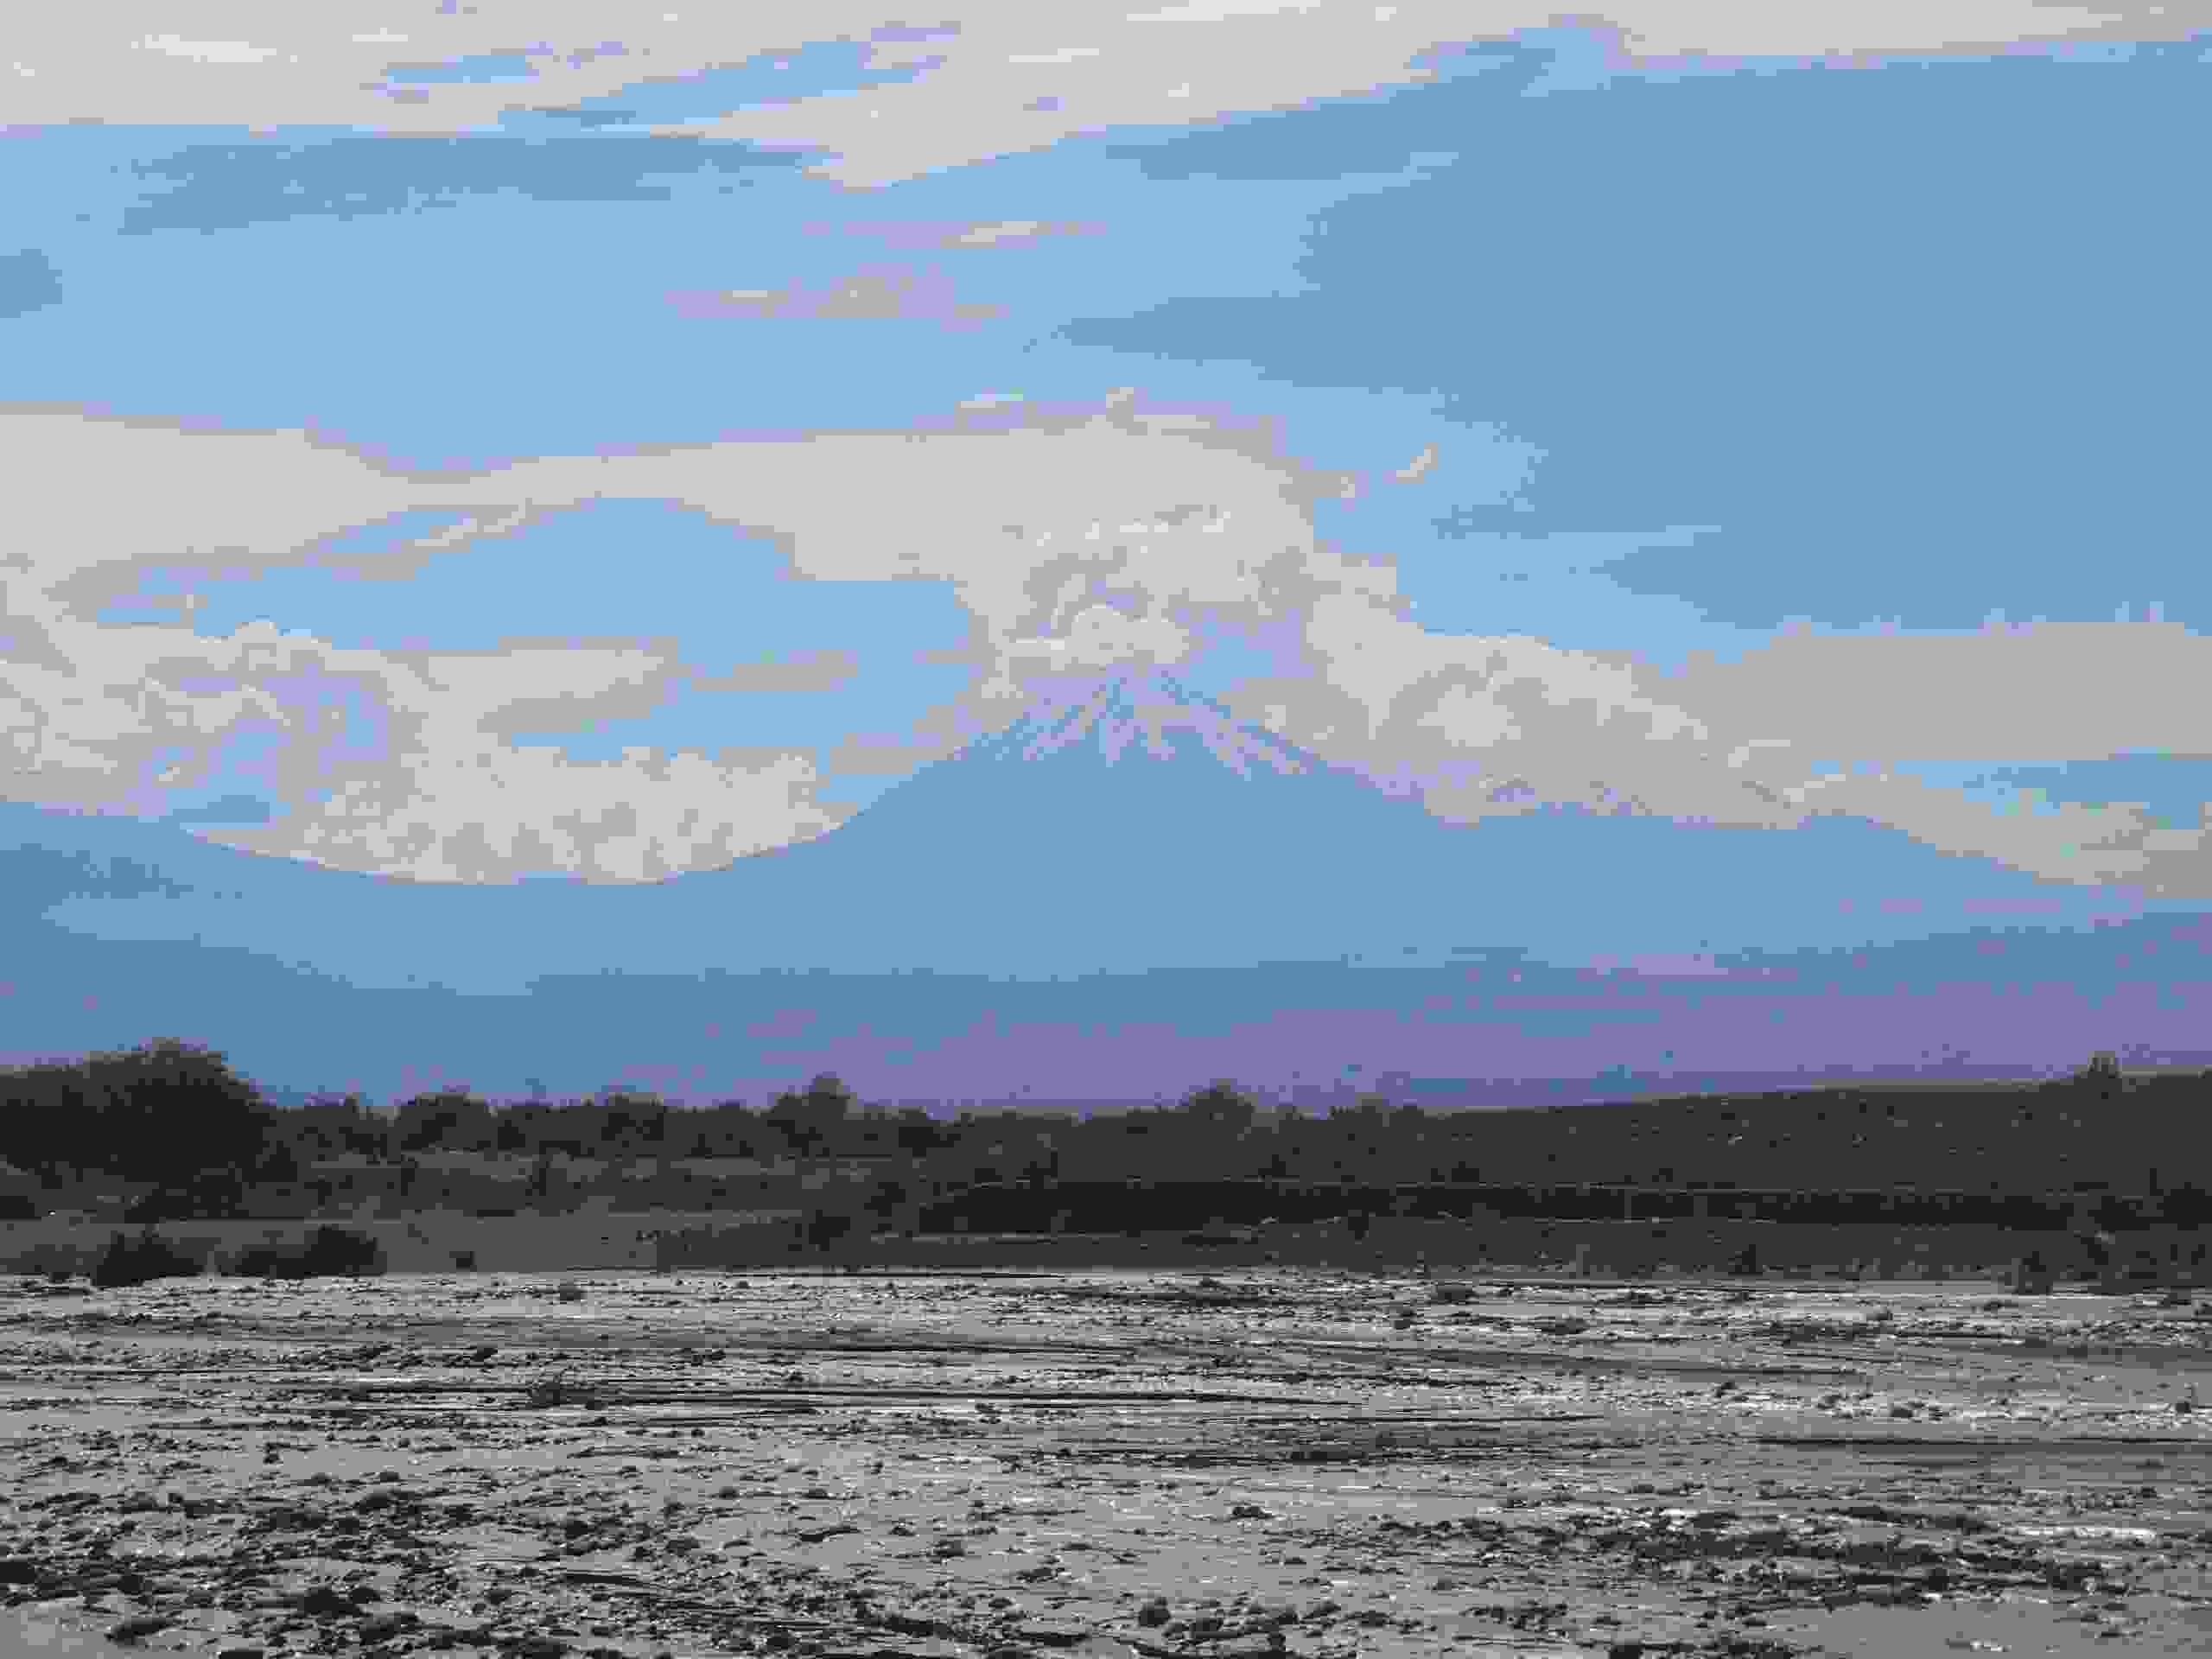
\includegraphics[width=\mywidth]{../wp-content/uploads/2015/04/wpid-wp-1427984374256.jpg} } 
 \newline
 Excursion à la vallée de la Lune toute proche. \newline
 \newline
\centerline{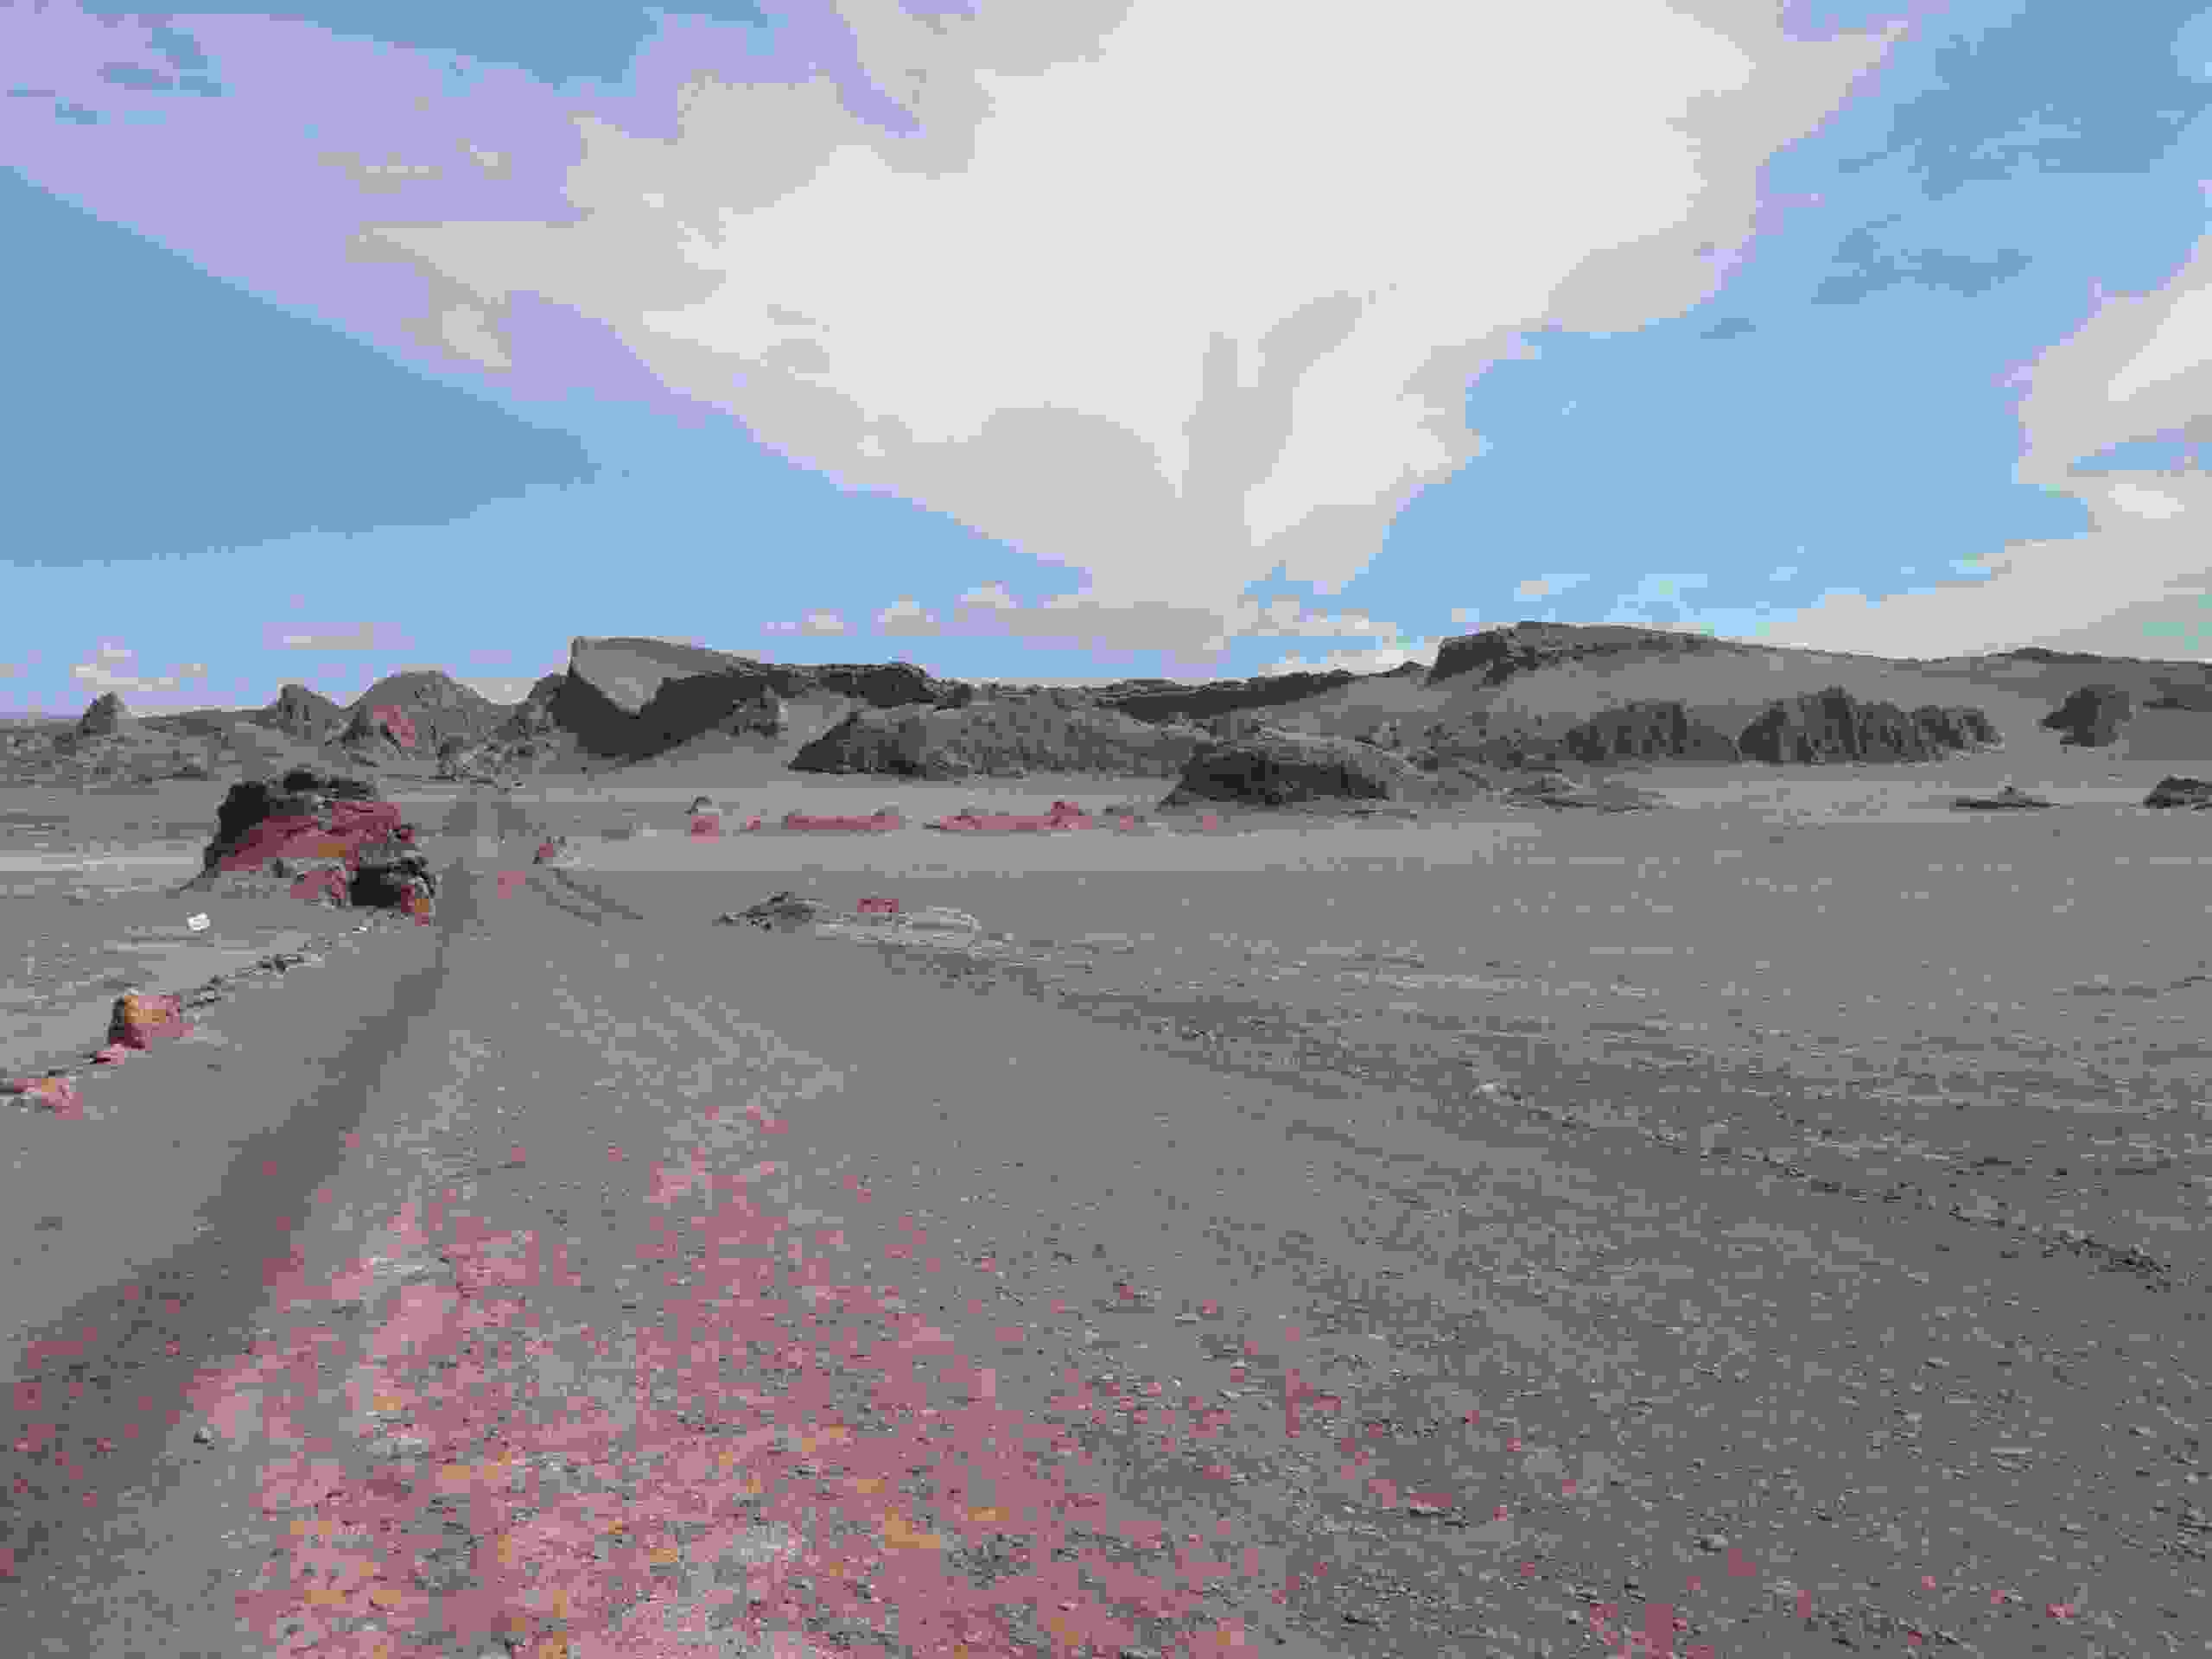
\includegraphics[width=\mywidth]{../wp-content/uploads/2015/04/wpid-wp-1427984406866.jpg} } 
 \newline
 \newline
\centerline{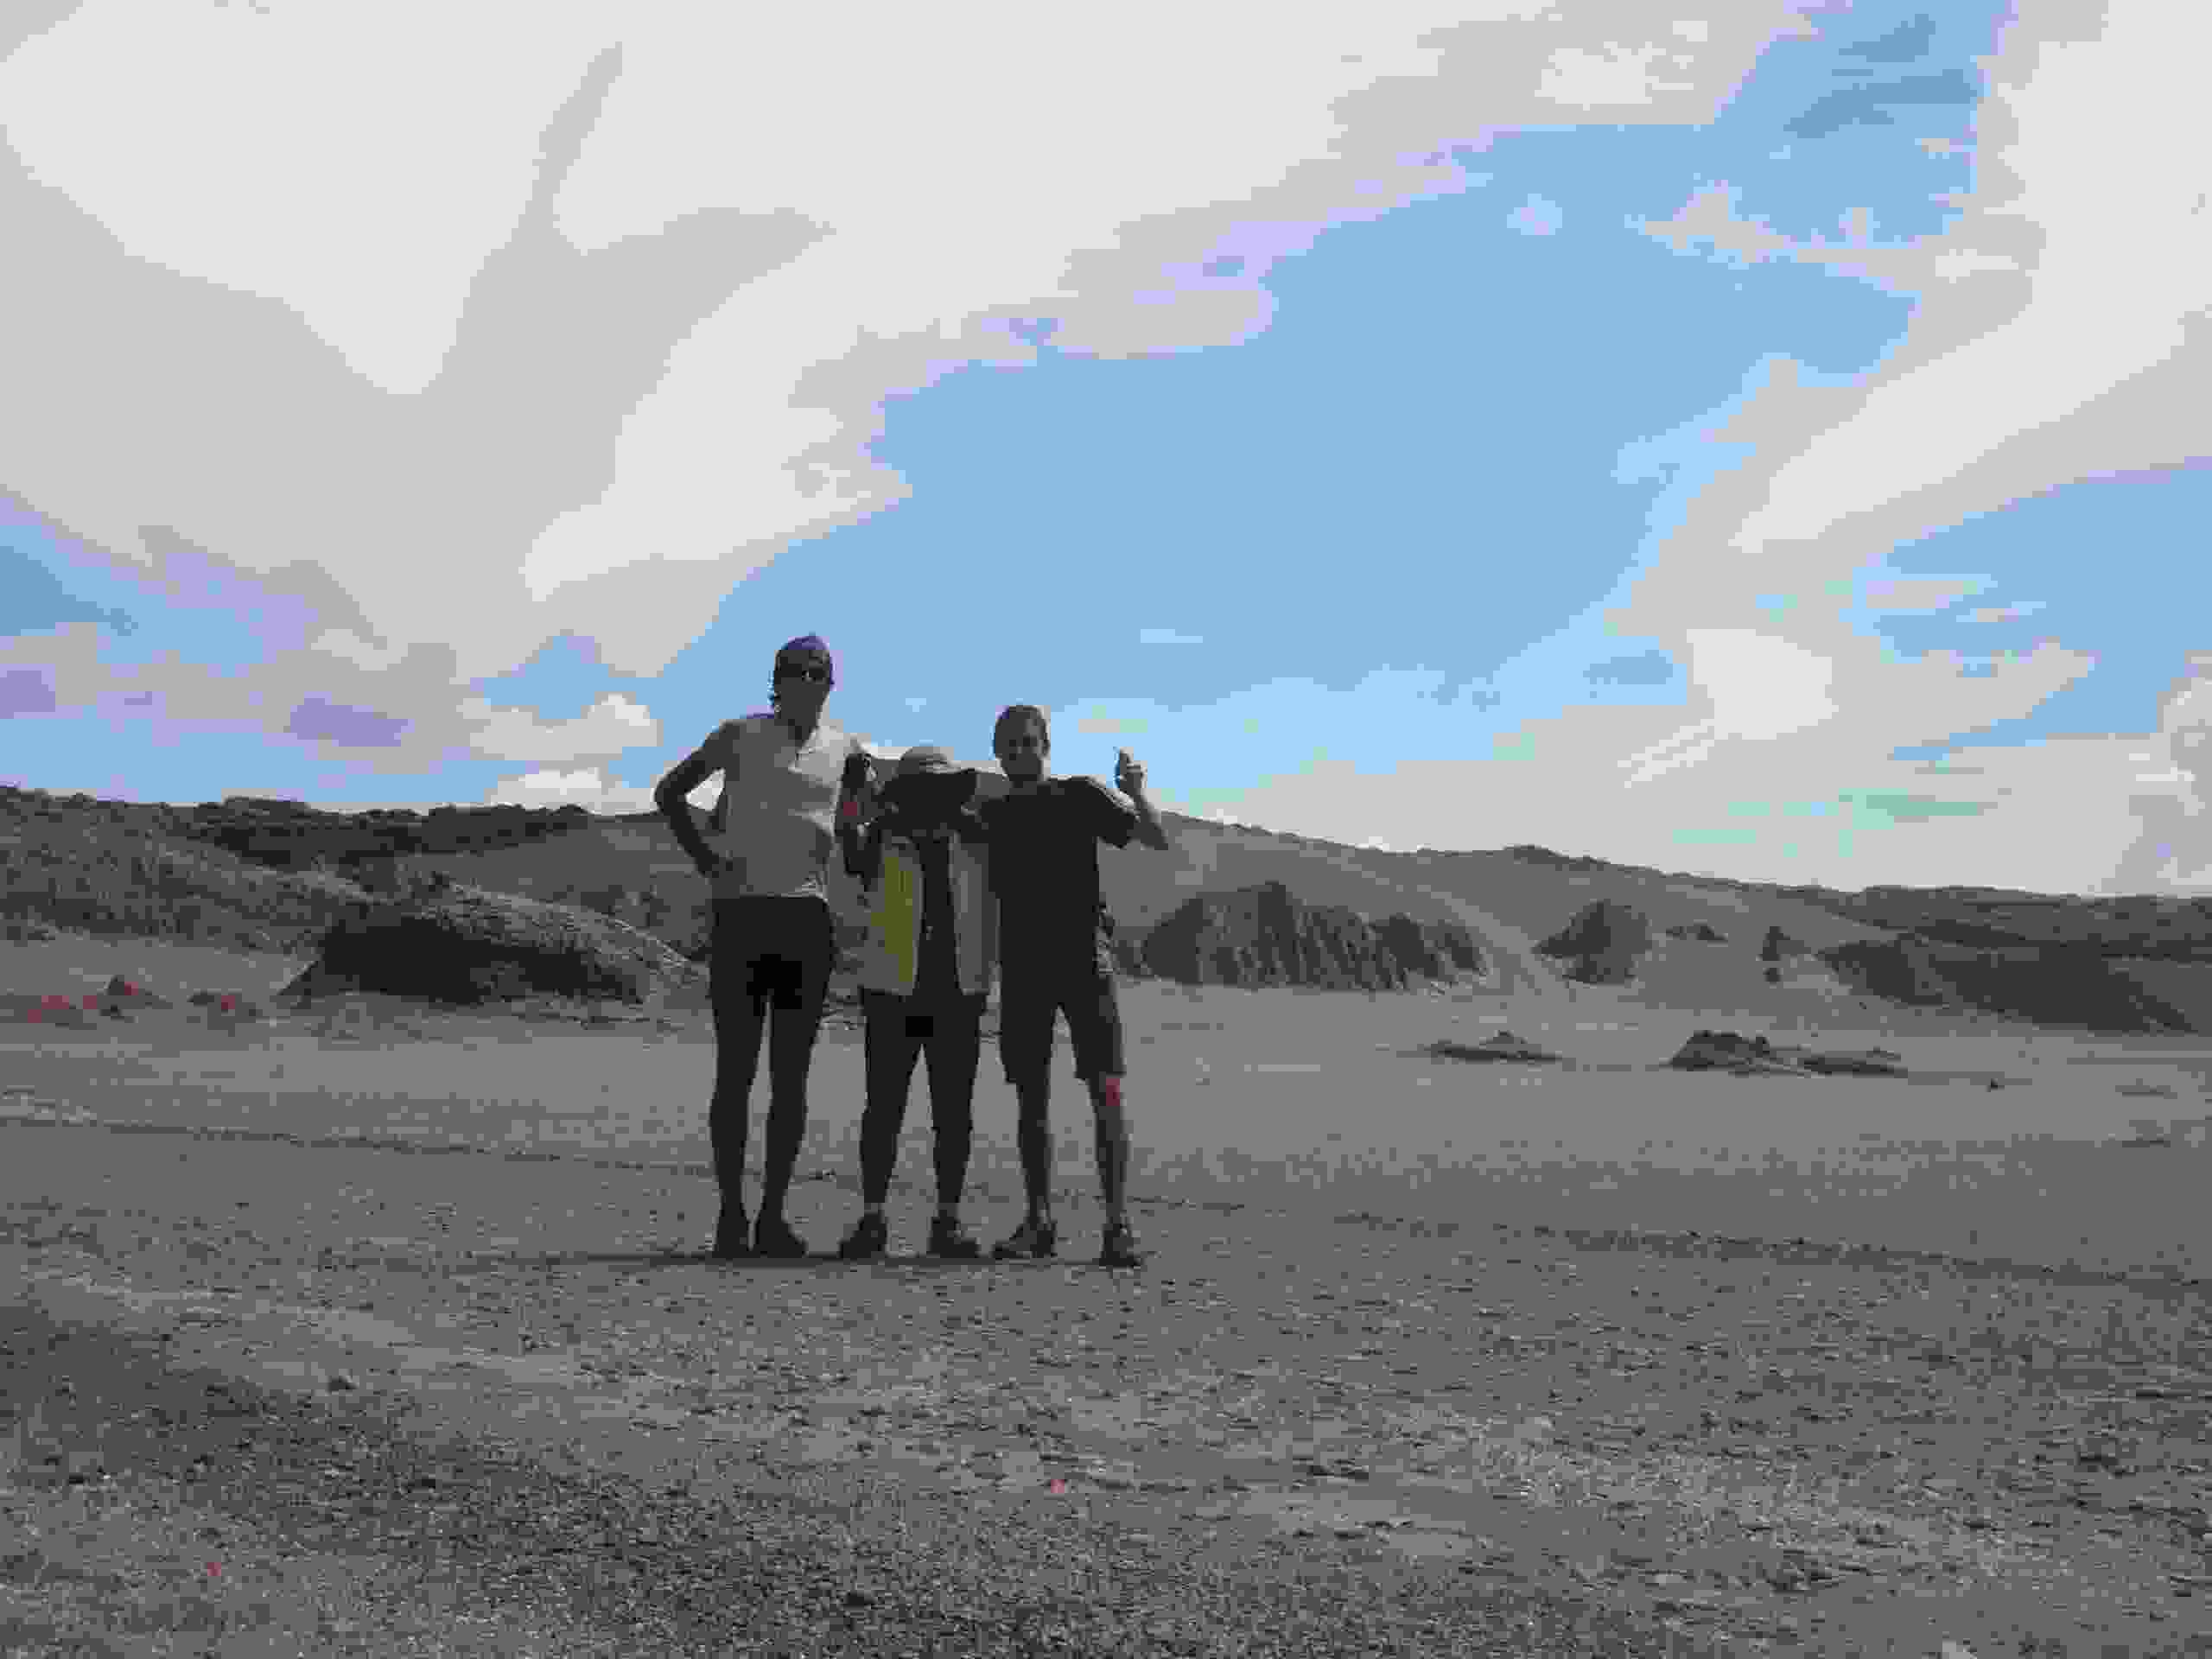
\includegraphics[width=\mywidth]{../wp-content/uploads/2015/04/wpid-wp-1427984342120.jpg} } 
 \newline
 Puis préparation de la suite : la traversée du Sud Lipez en Bolivie, en compagnie de Lucie et Frédéric qui ont le même itinéraire. \newline
 D'abord aller chercher des infos sur l'état des pistes et la météo auprès des agences de tour en jeep, puis faire le plein de nourriture pour une dizaine de jours d'autonomie. \newline
 \newline
\centerline{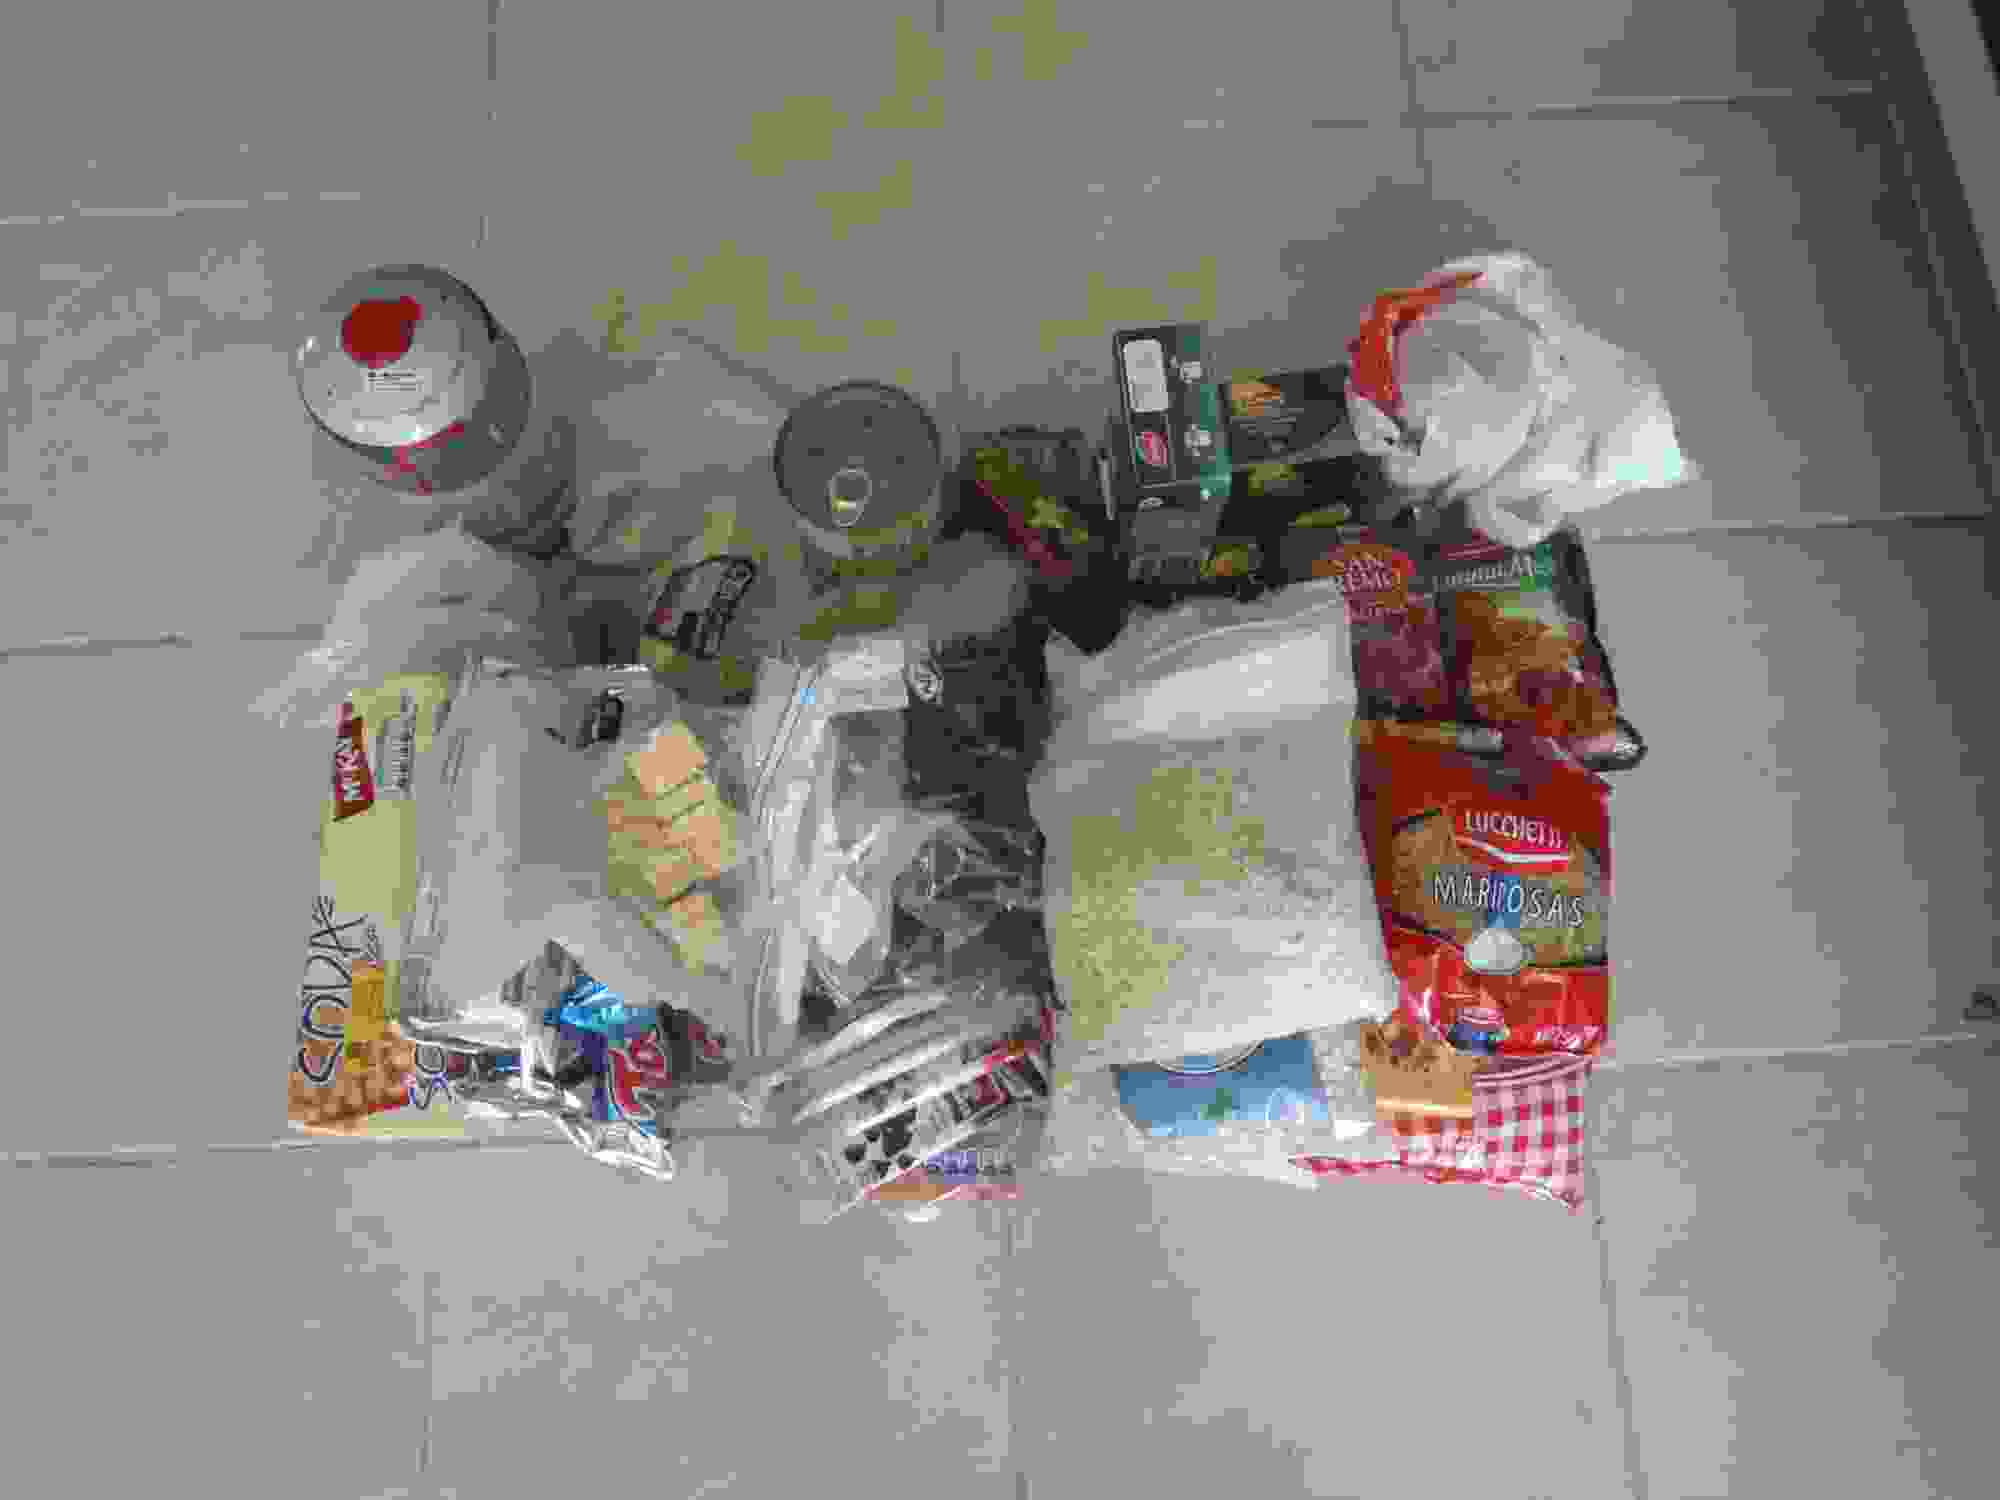
\includegraphics[width=\mywidth]{../wp-content/uploads/2015/04/wpid-wp-1427986446964.jpg} } 
 \newline
 1er jour : \newline
 Passage à la douane chilienne et montée à 4600m à la frontière bolivienne à l'entrée du Sud Lipez : en stop dans un camping car de touristes américains, pas besoin de s'épuiser d'entrée la suite sera assez difficile. \newline
 \newline
\centerline{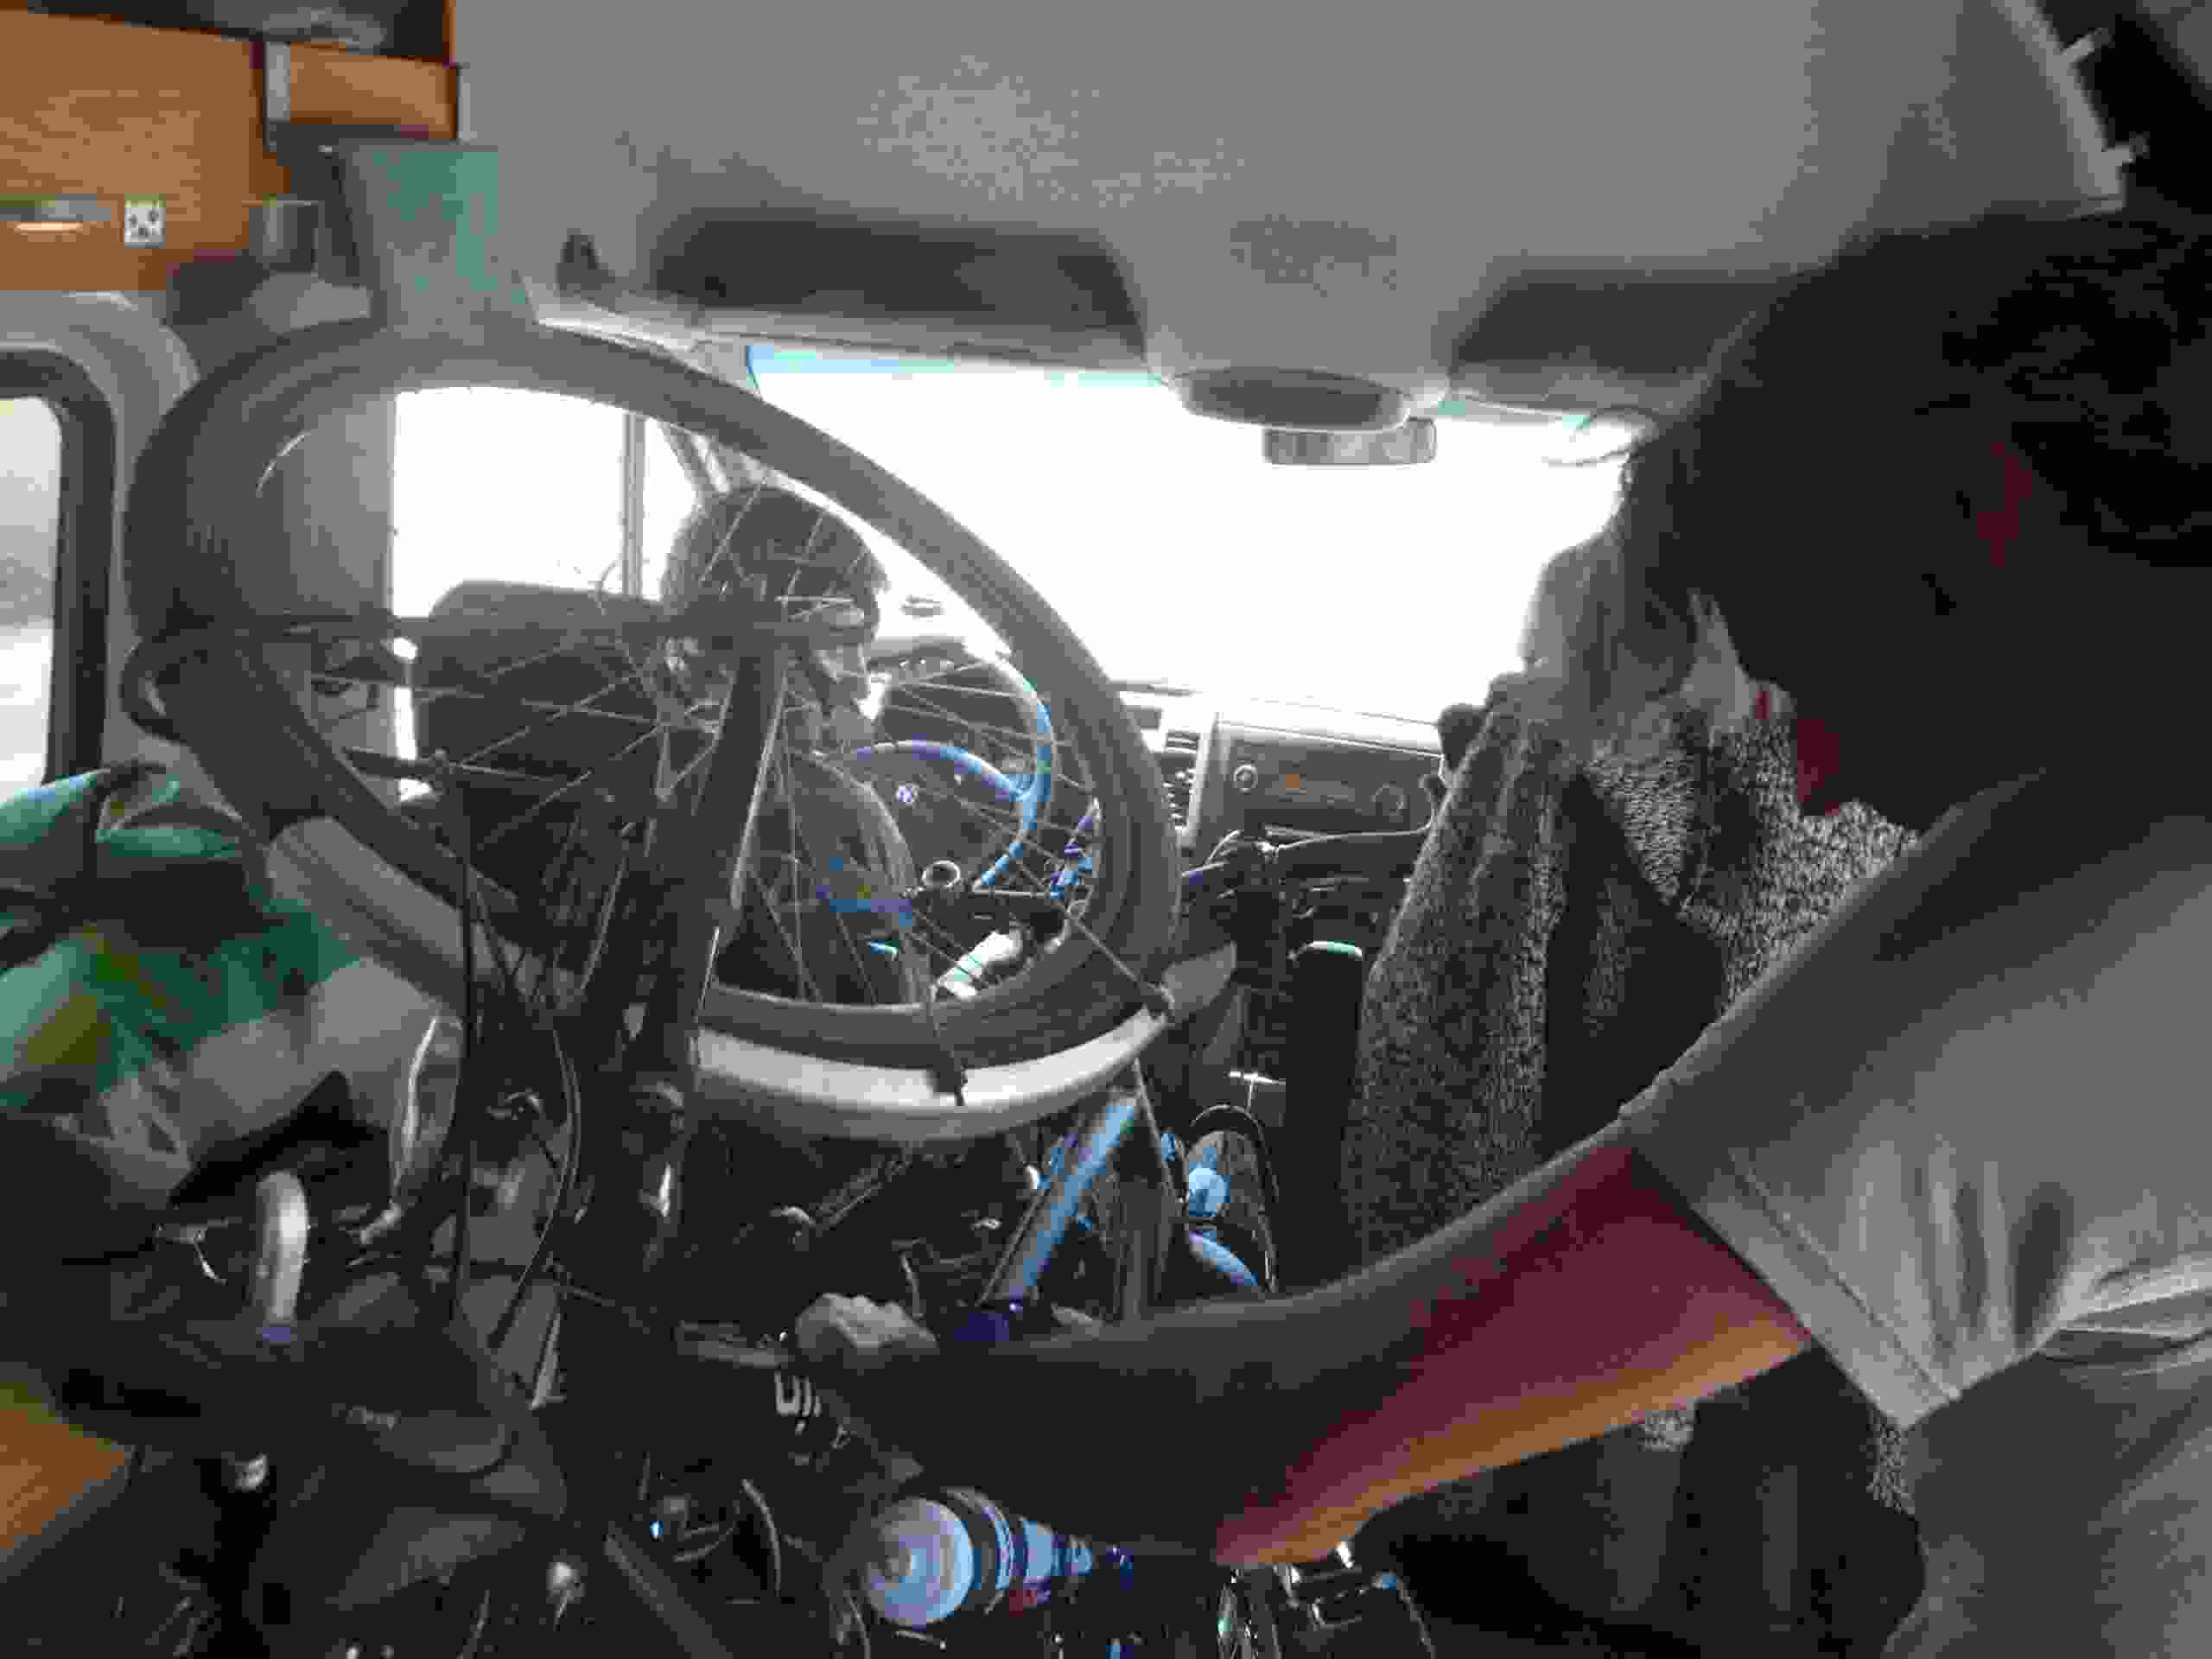
\includegraphics[width=\mywidth]{../wp-content/uploads/2015/04/wpid-wp-1427943860712.jpg} } 
 \newline
 \newline
\centerline{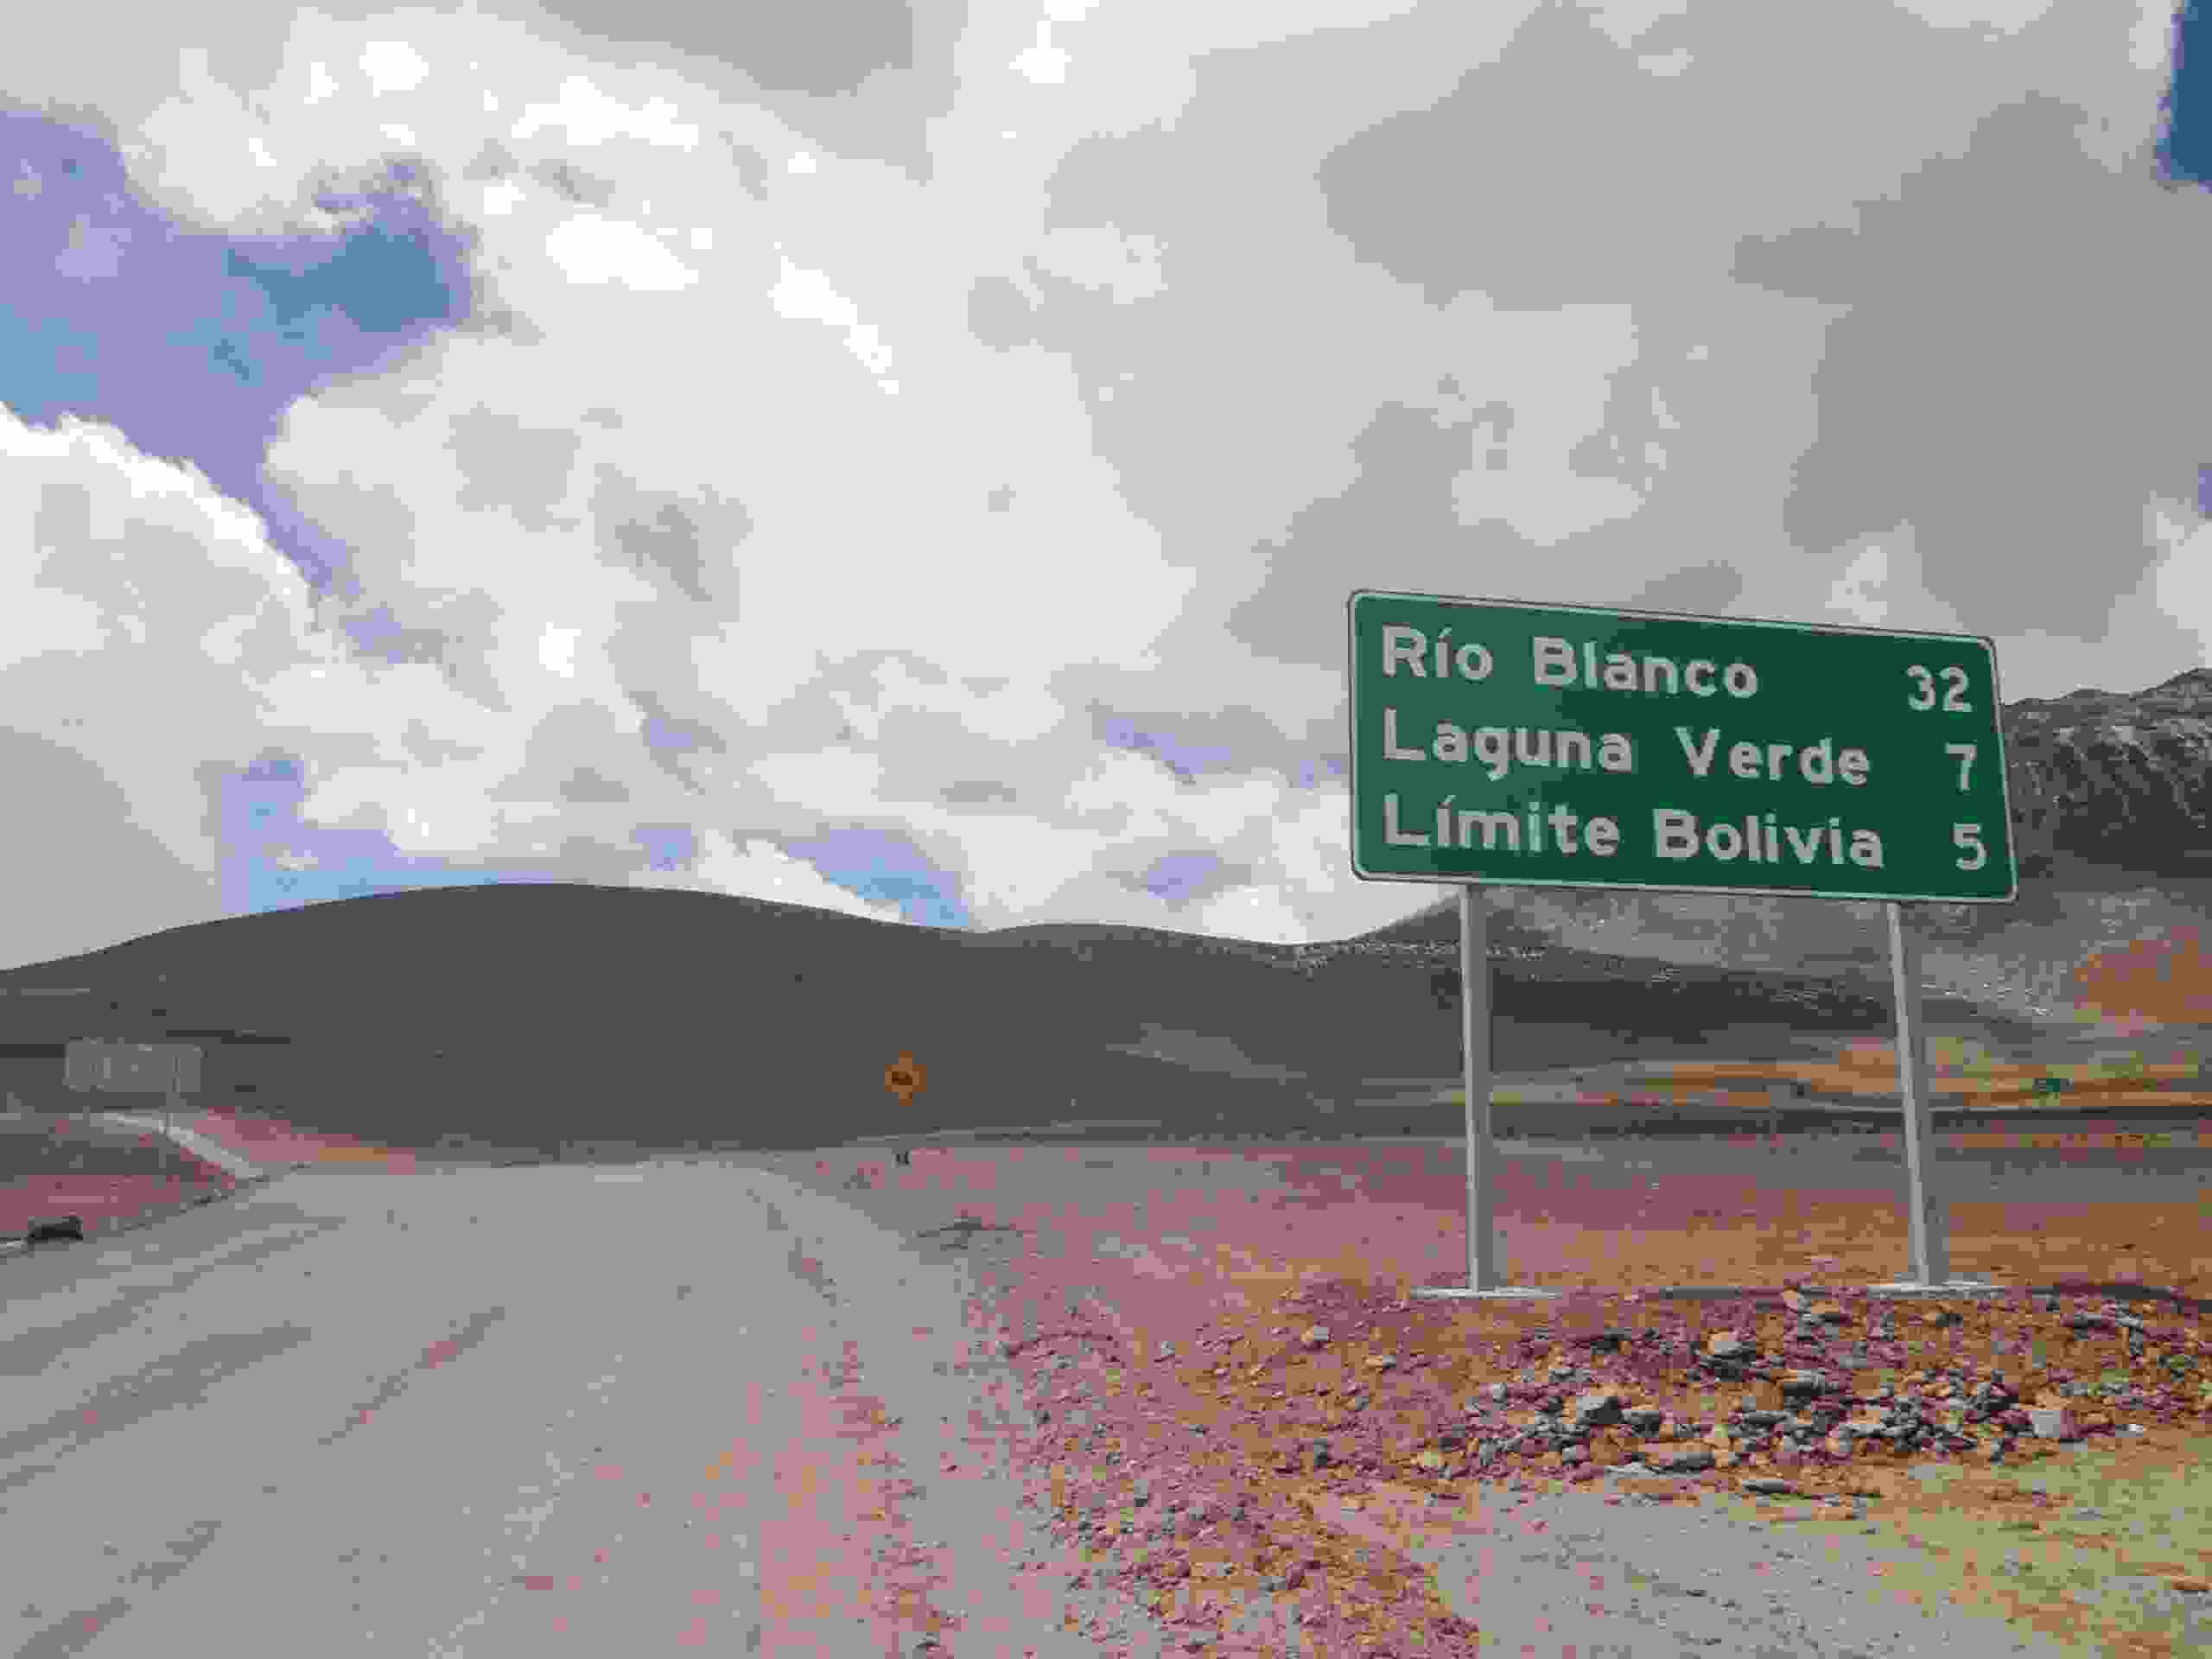
\includegraphics[width=\mywidth]{../wp-content/uploads/2015/04/wpid-wp-1427943860696.jpg} } 
 \newline
 On arrive assez rapidement à la Laguna Blanca puis à la Laguna Verde. \newline
 \newline
\centerline{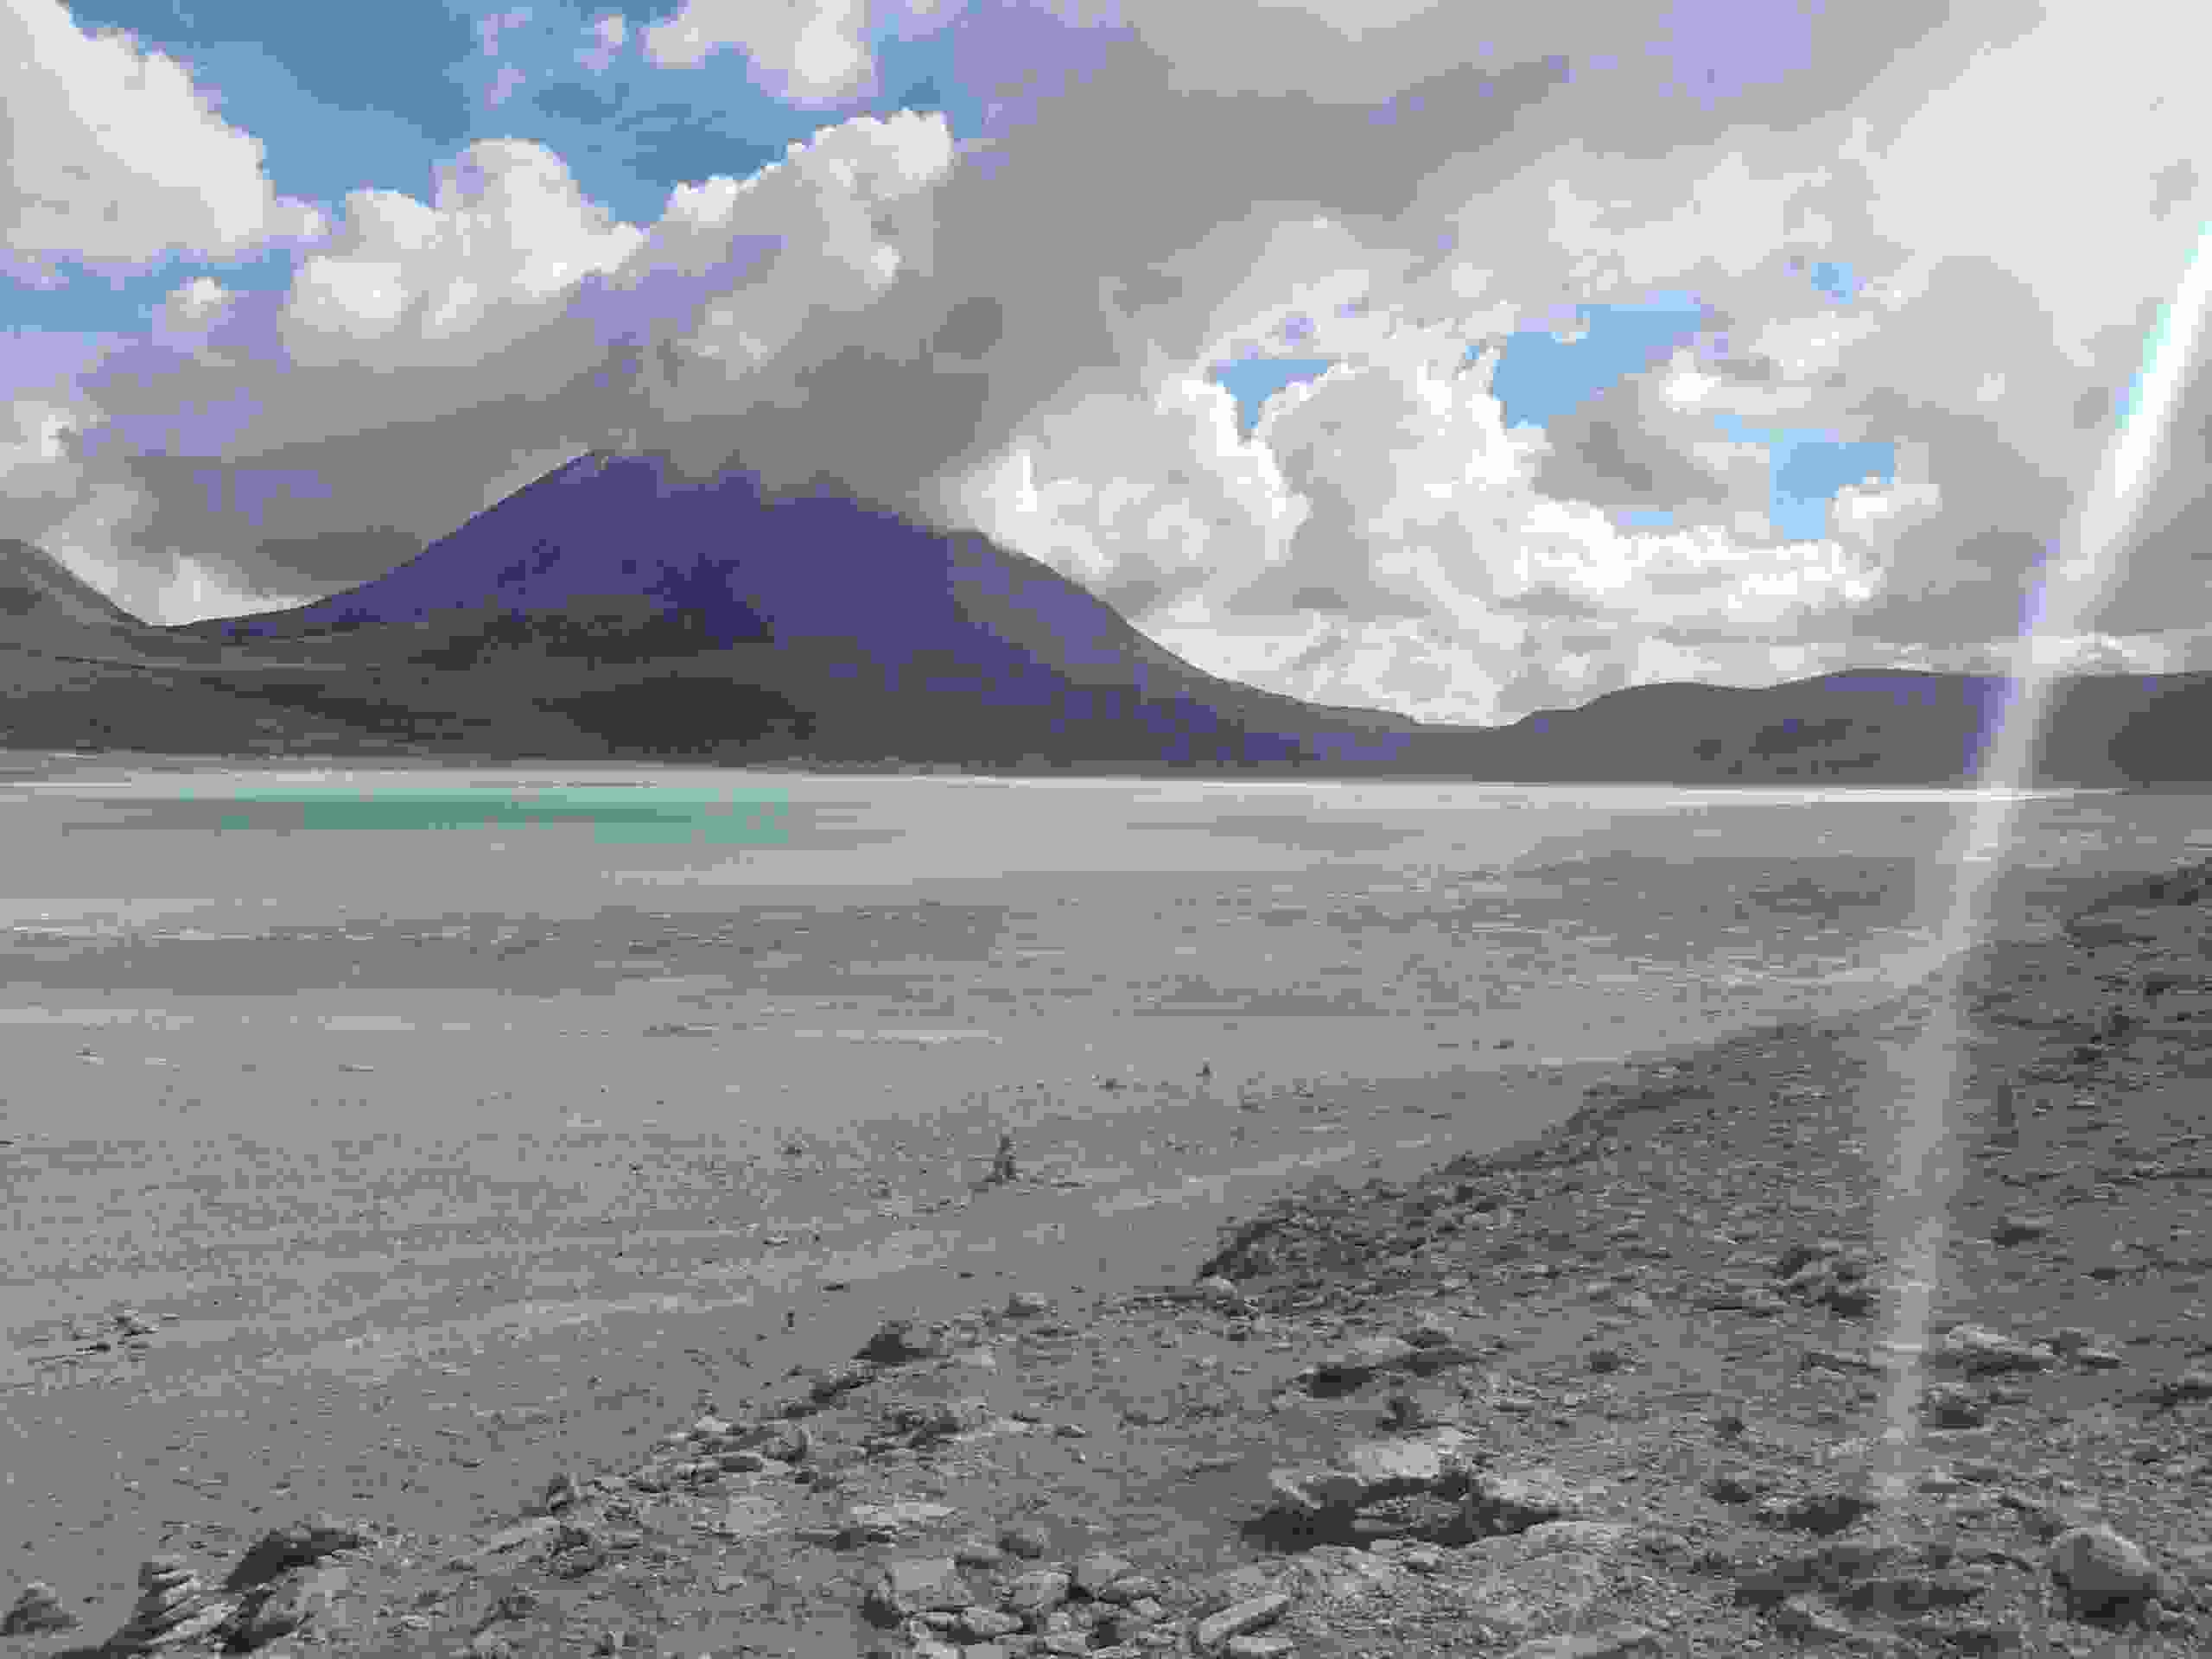
\includegraphics[width=\mywidth]{../wp-content/uploads/2015/04/wpid-wp-1427943860676.jpg} } 
 \newline
 \newline
\centerline{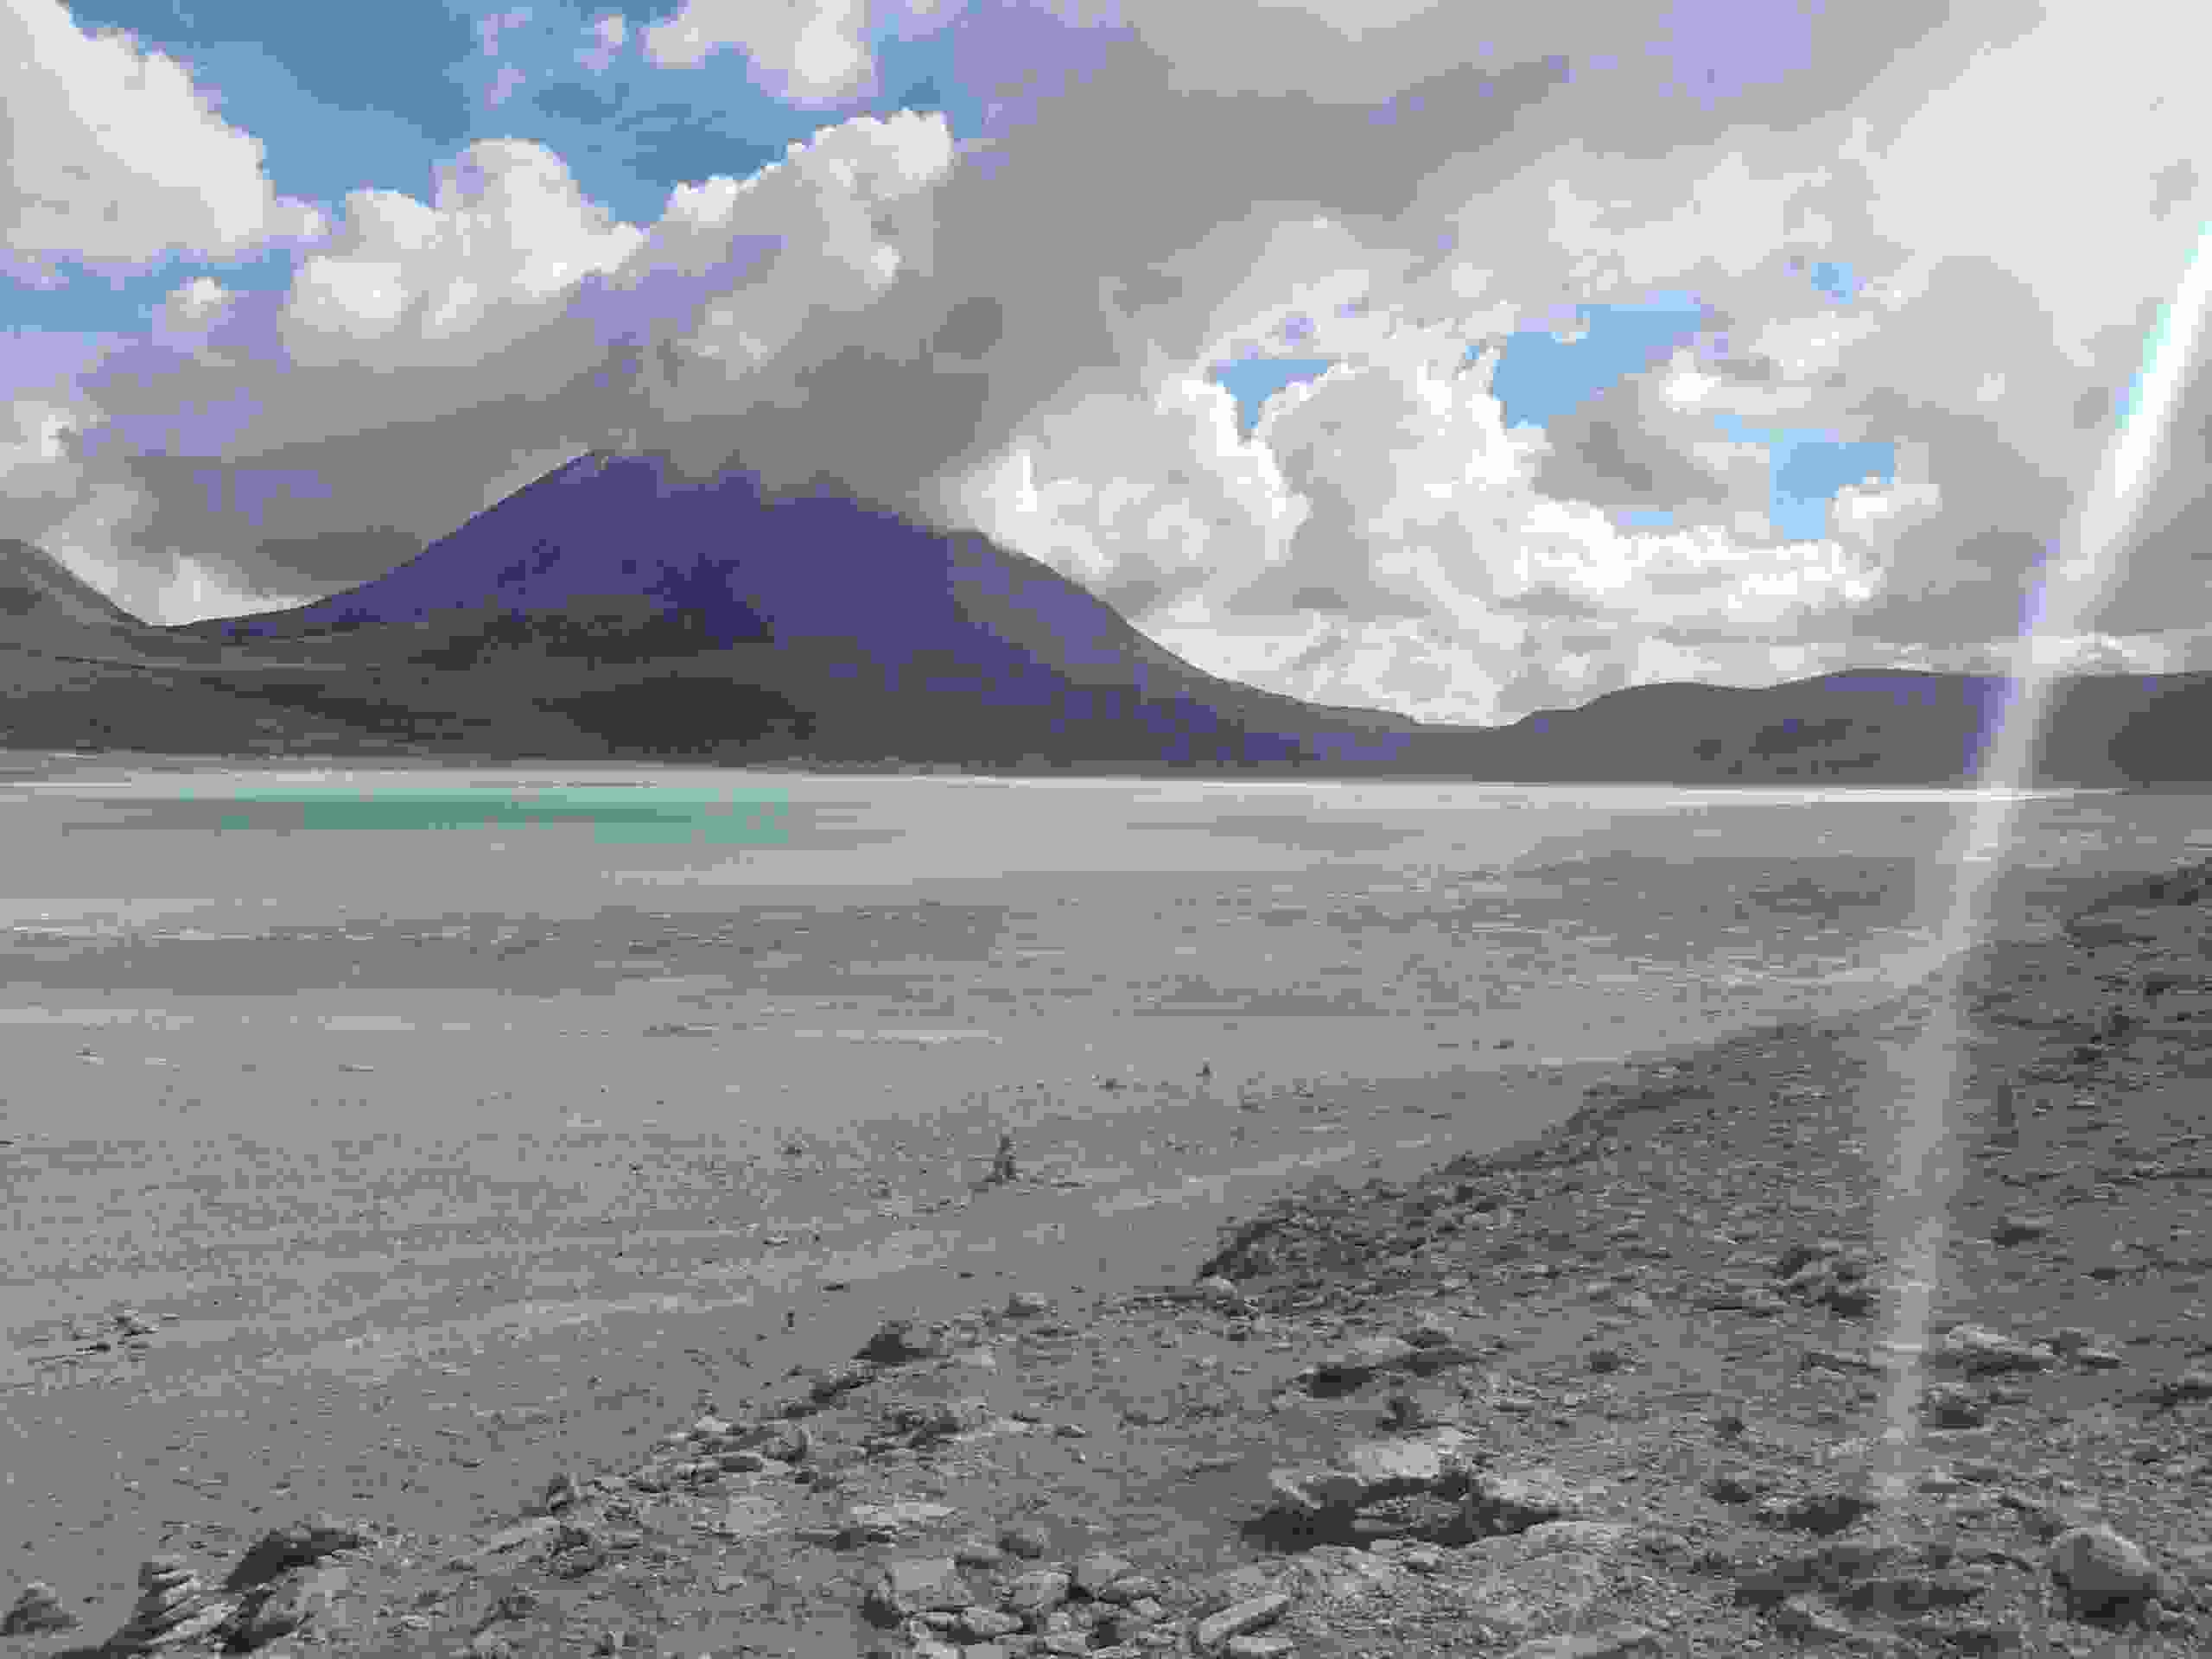
\includegraphics[width=\mywidth]{../wp-content/uploads/2015/04/wpid-wp-1427983994198.jpg} } 
 \newline
 Bivouac dans une maison en ruine. \newline
 \newline
\centerline{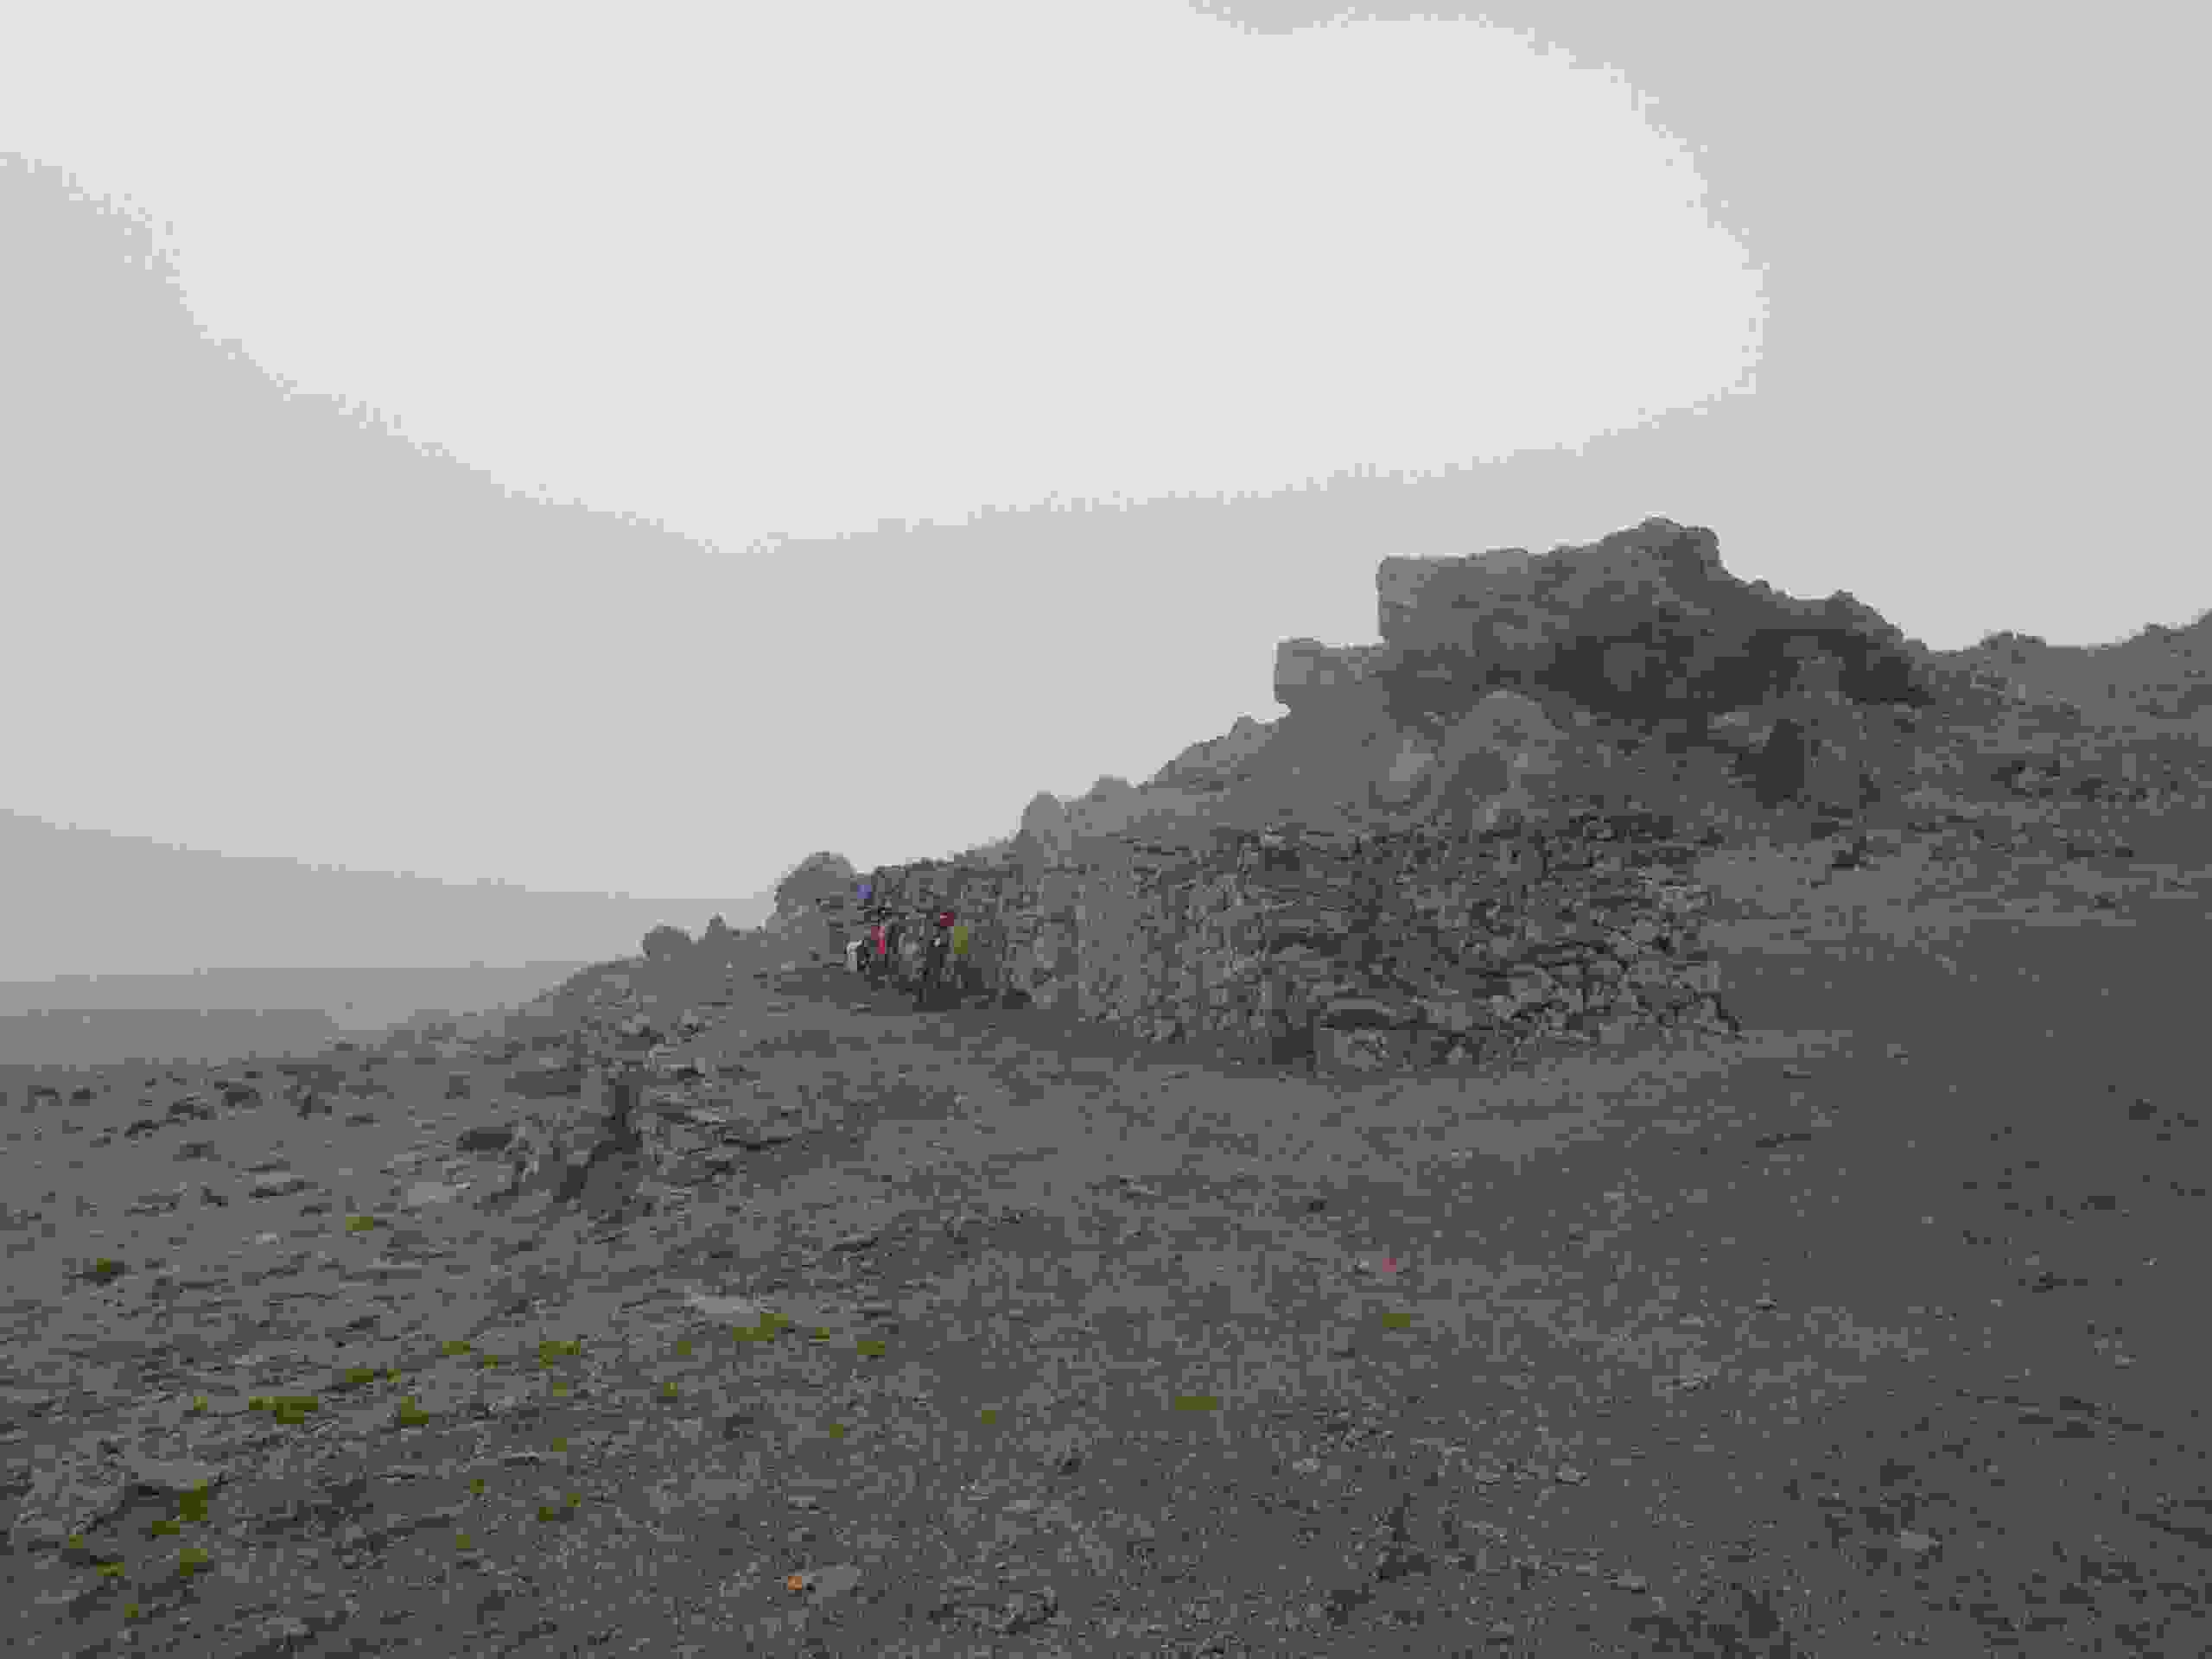
\includegraphics[width=\mywidth]{../wp-content/uploads/2015/04/wpid-wp-1427984018829.jpg} } 
 \newline
 2e jour : \newline
 Lever dans la brume, les jeeps de touristes passent devant nous. \newline
 \newline
\centerline{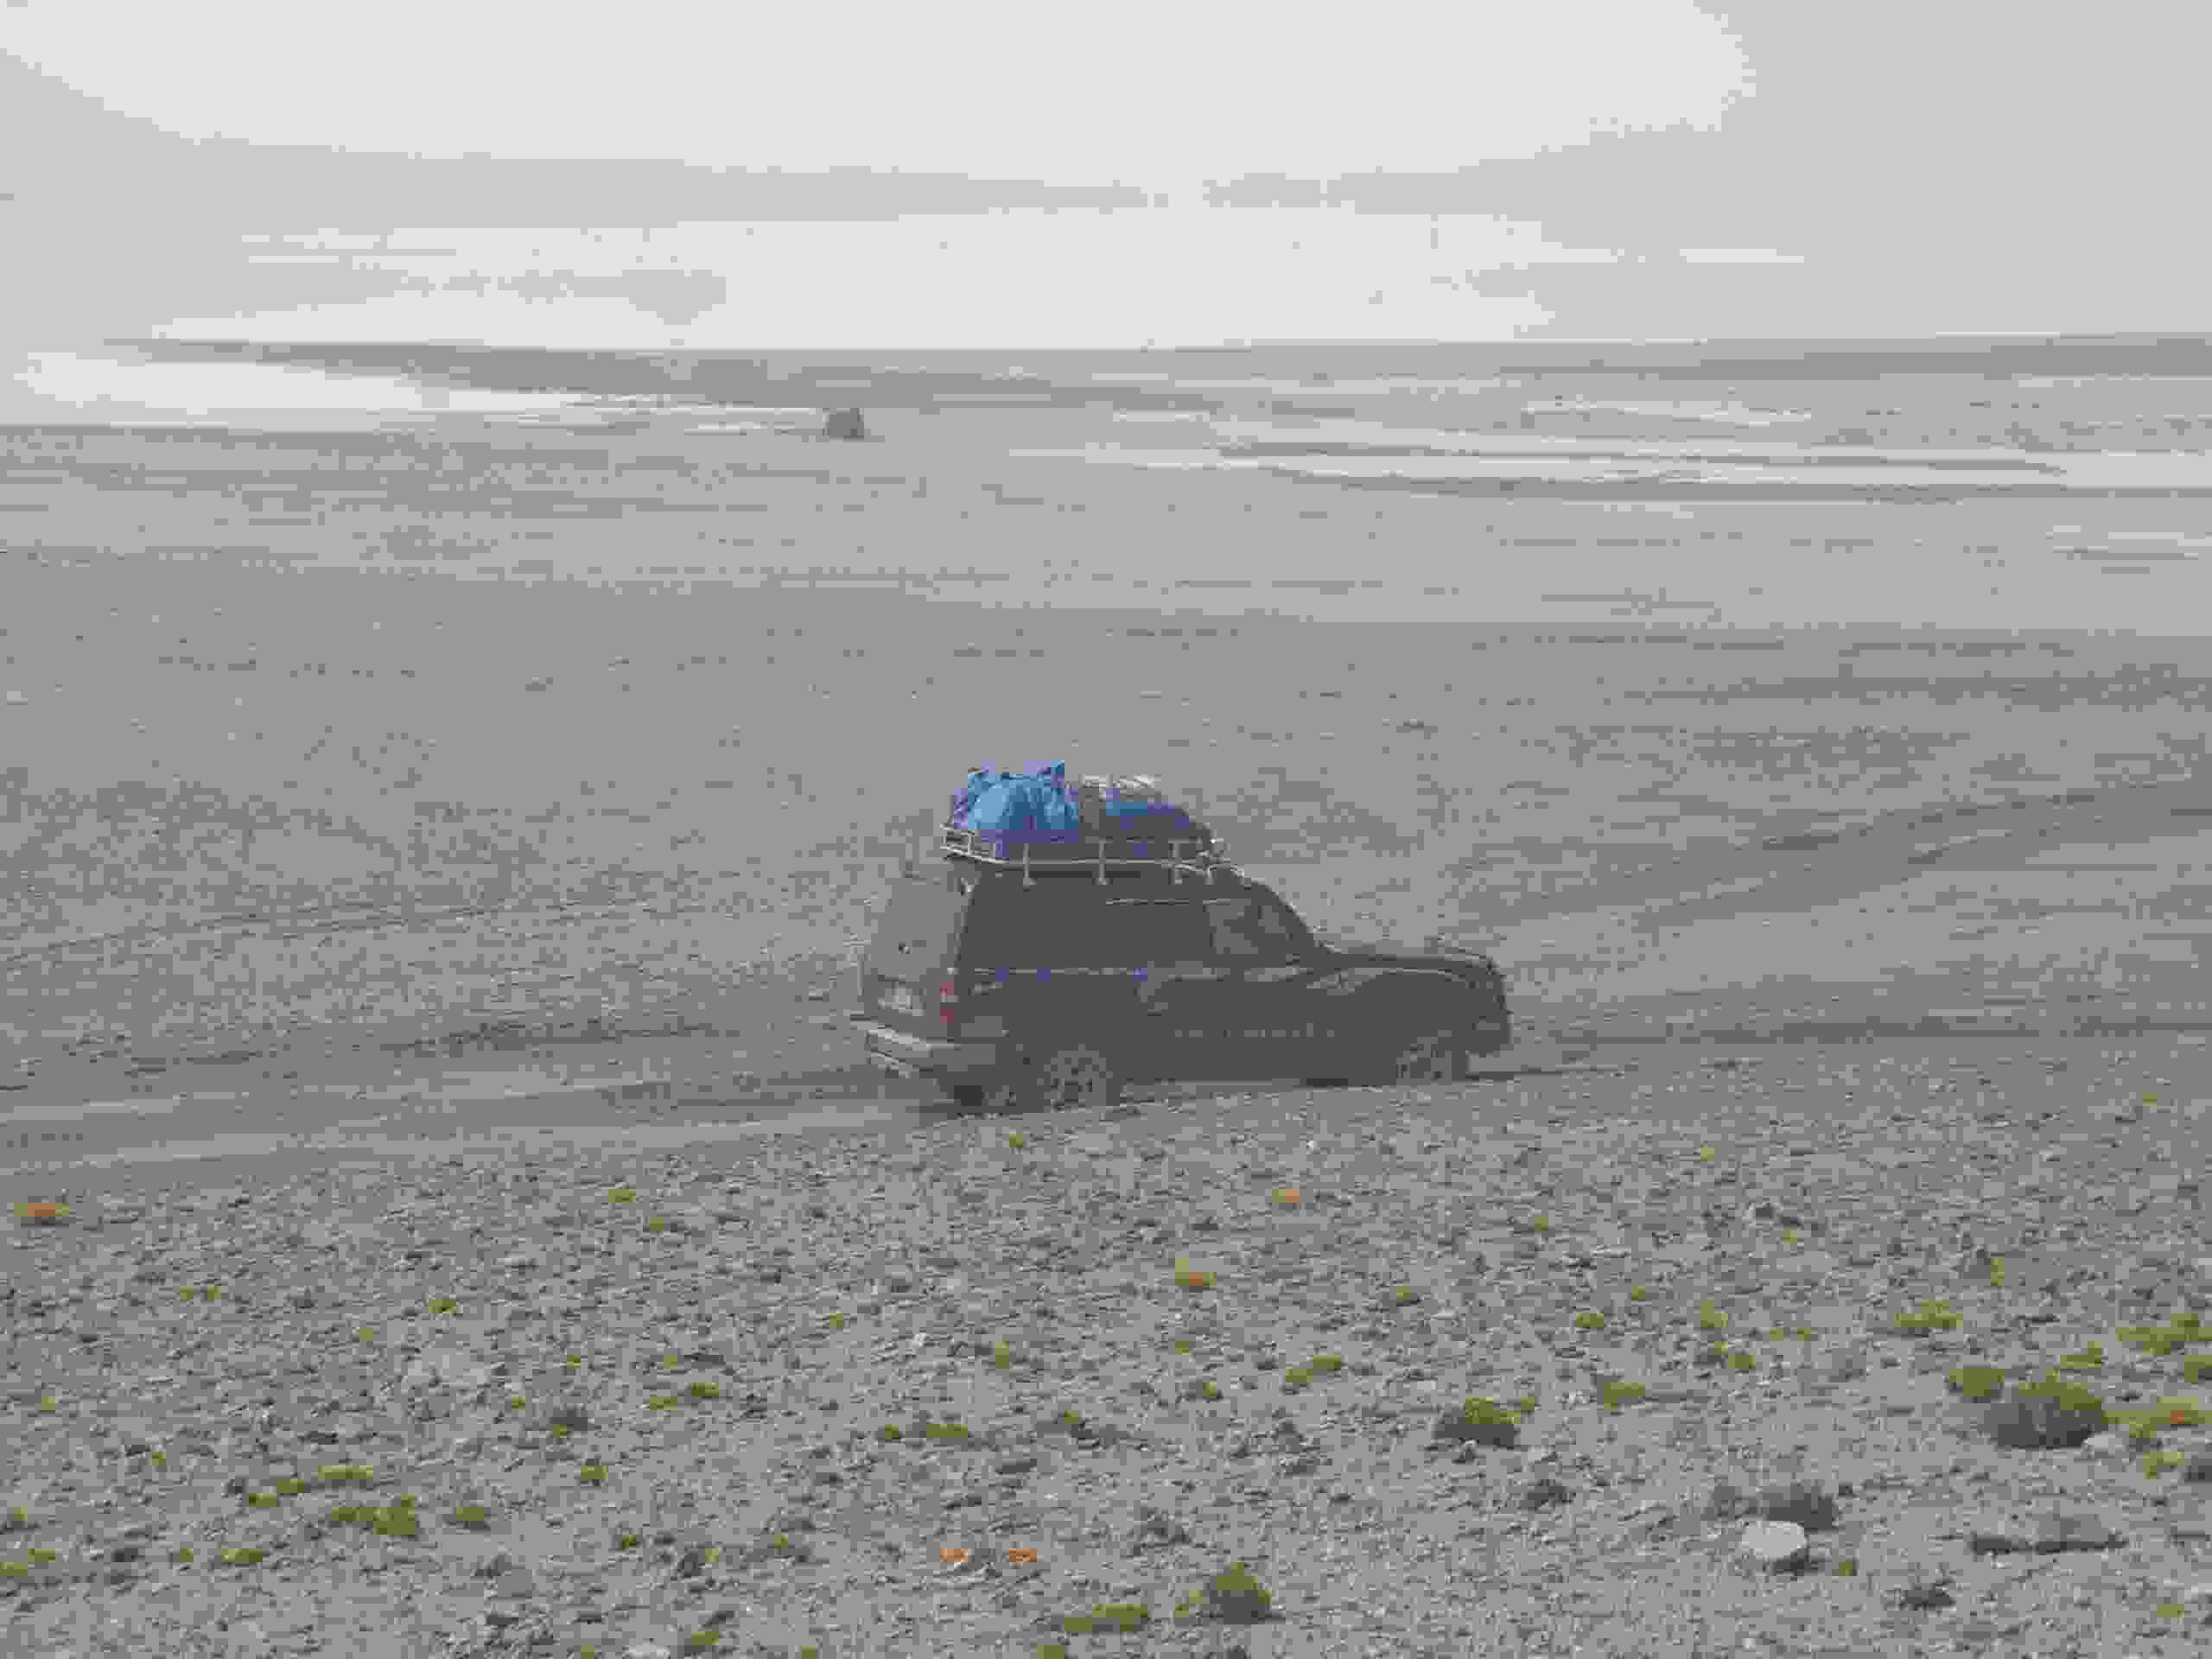
\includegraphics[width=\mywidth]{../wp-content/uploads/2015/04/wpid-wp-1427984048275.jpg} } 
 \newline
 Ensuite beau temps, vent dans le dos, piste roulante et paysages magnifiques : le Sud Lipez s'annonce bien ! \newline
 \newline
\centerline{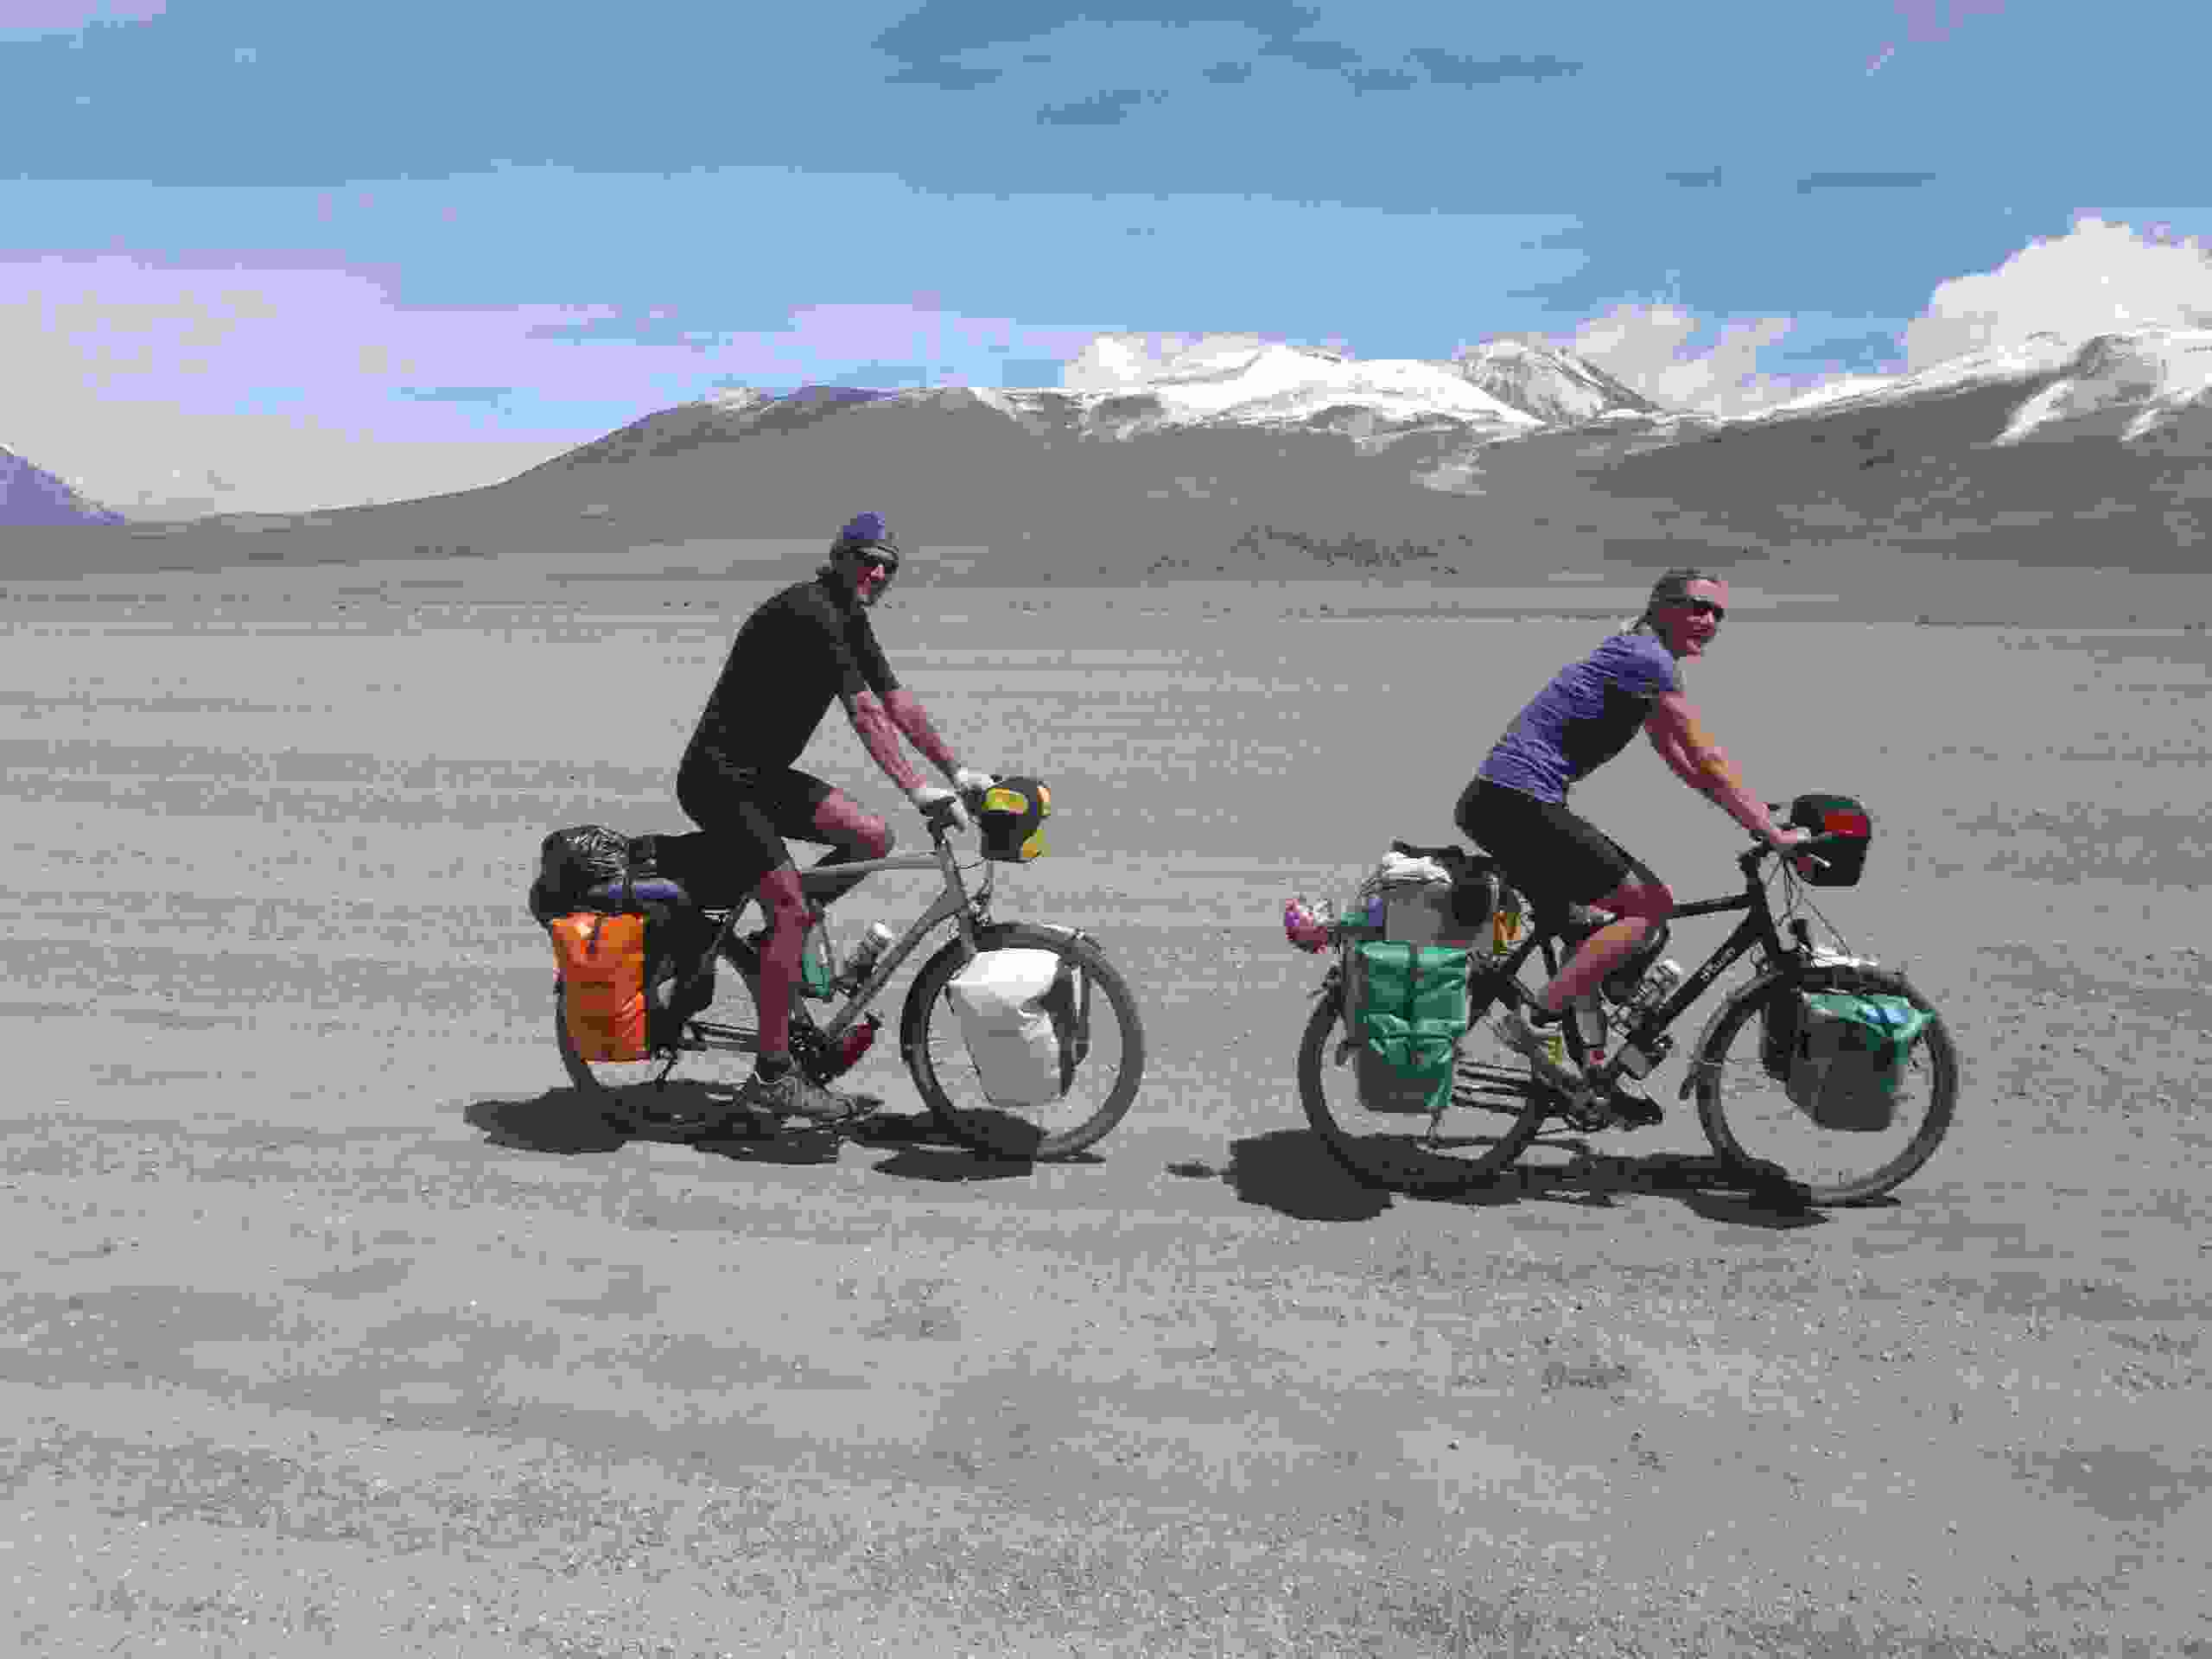
\includegraphics[width=\mywidth]{../wp-content/uploads/2015/04/wpid-wp-1427984125510.jpg} } 
 \newline
 \newline
\centerline{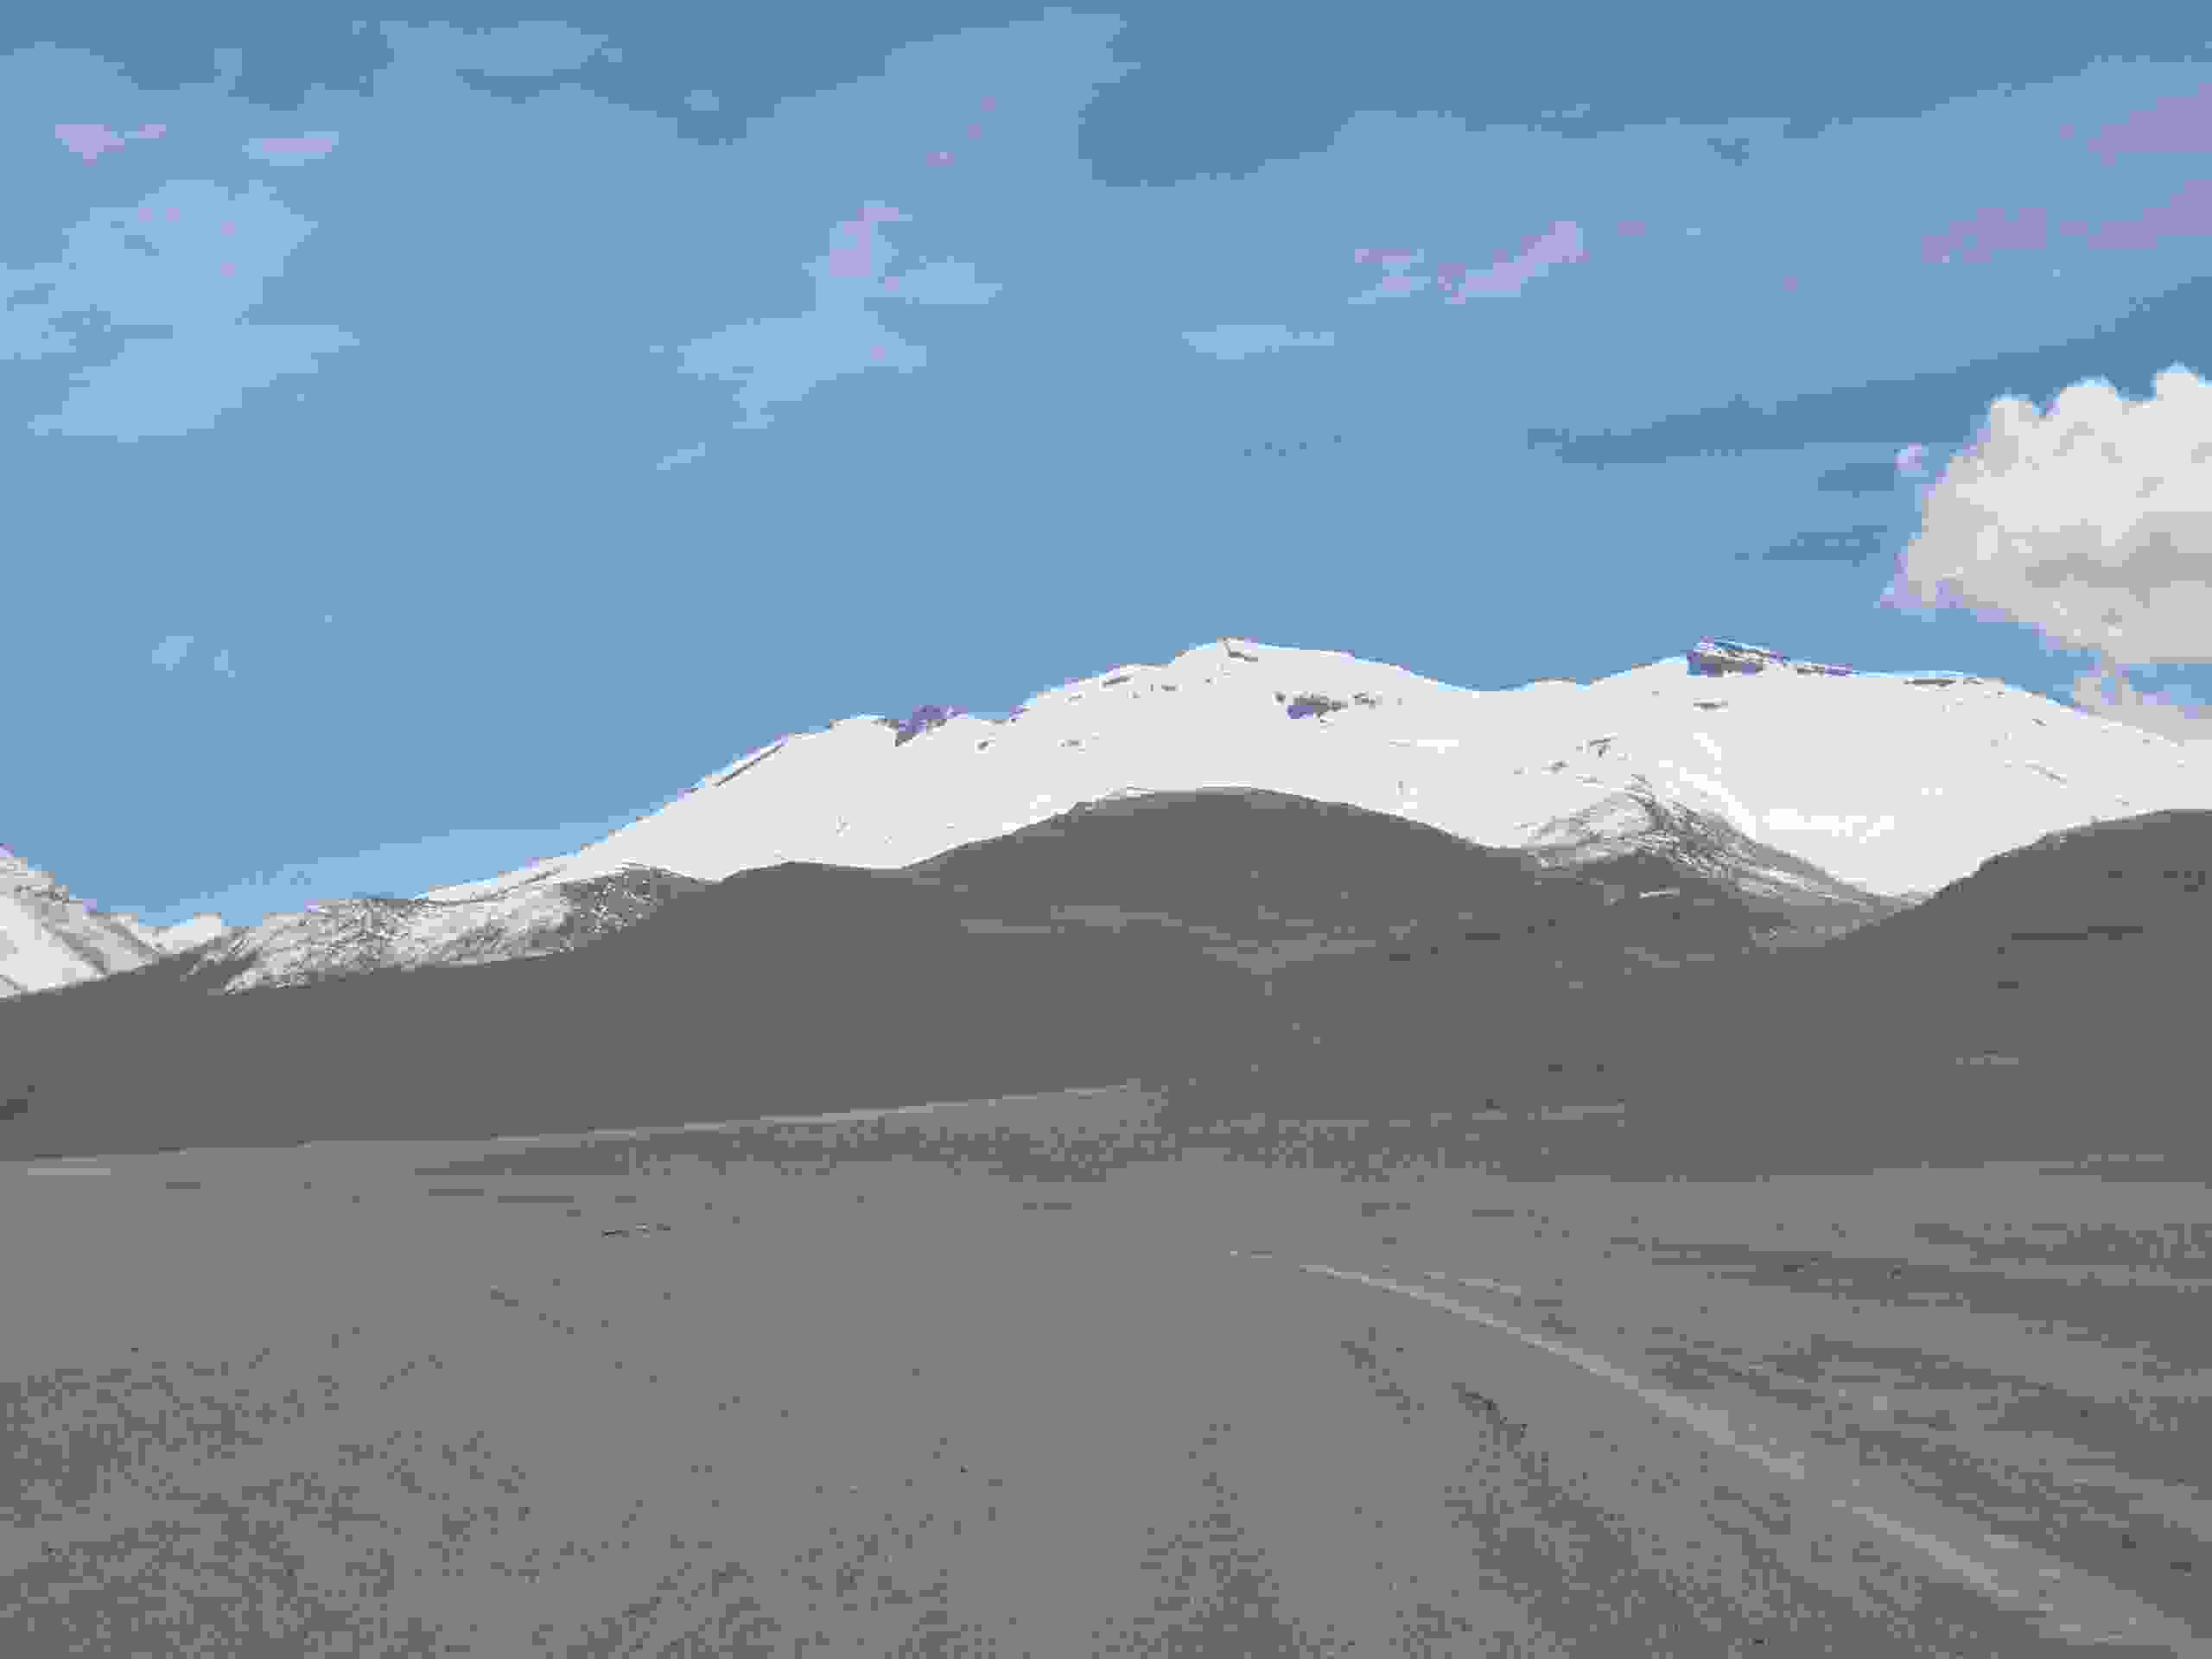
\includegraphics[width=\mywidth]{../wp-content/uploads/2015/04/wpid-wp-1427984230200.jpg} } 
 \newline
 \newline
\centerline{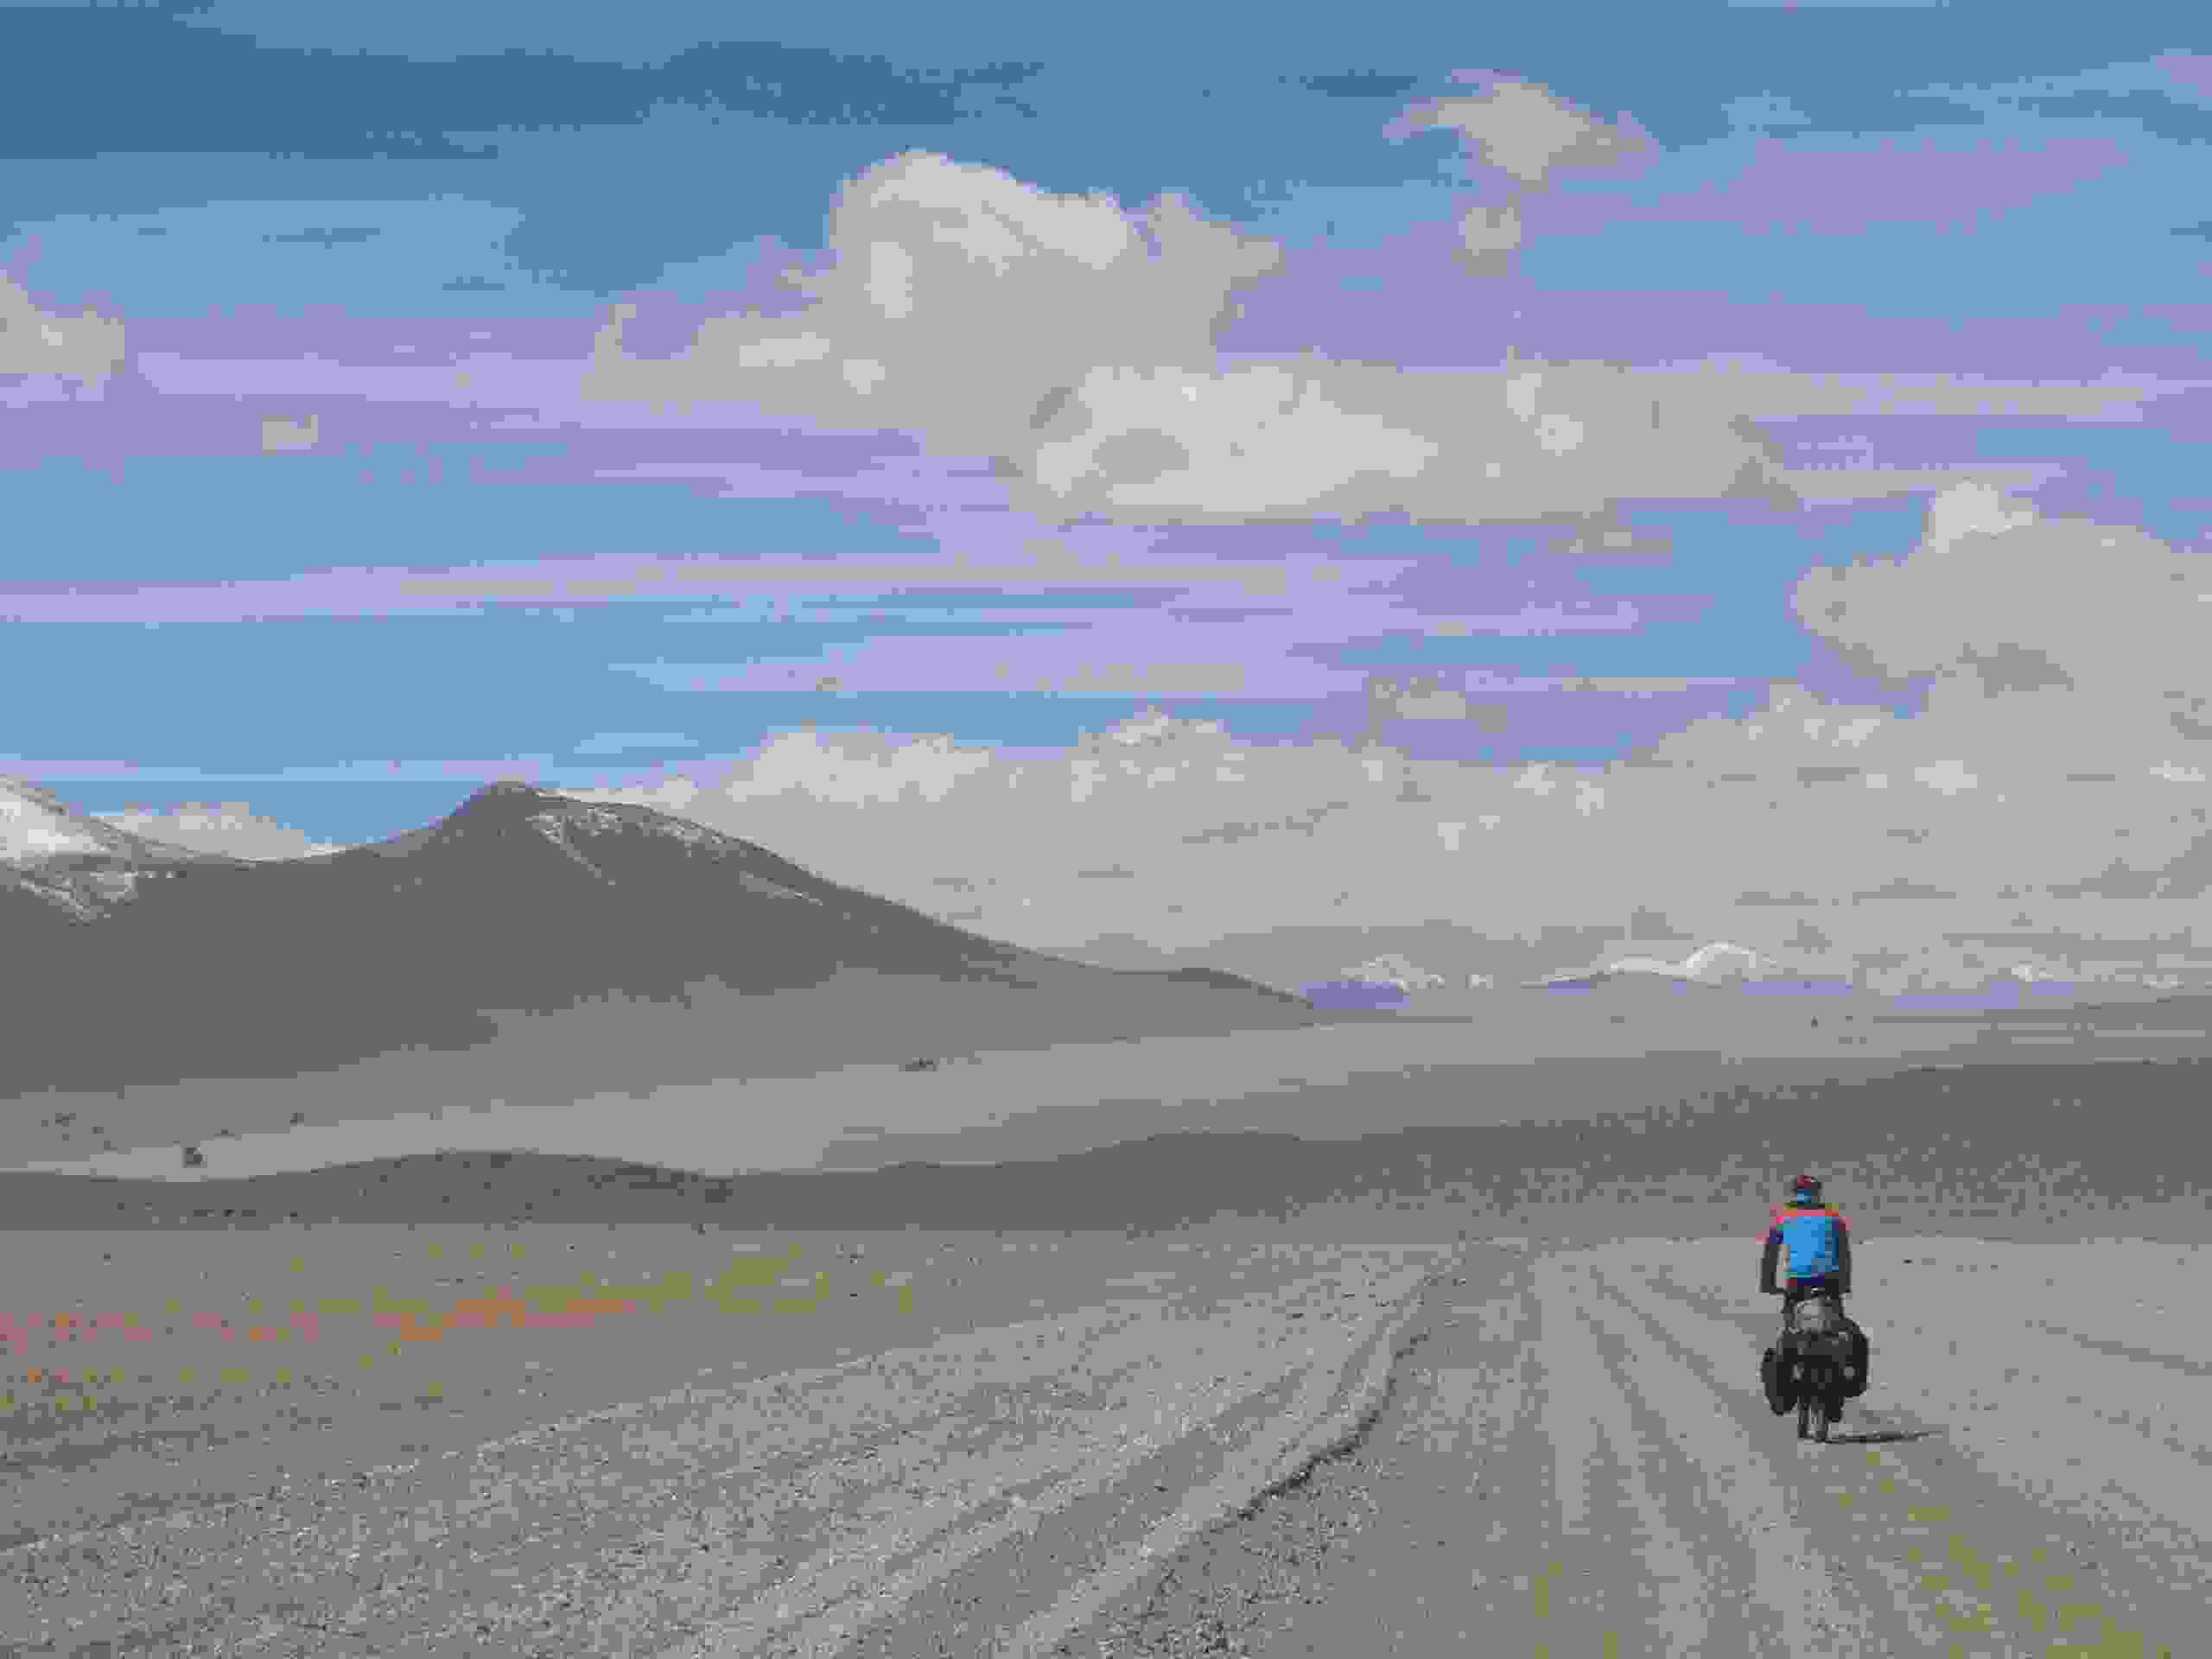
\includegraphics[width=\mywidth]{../wp-content/uploads/2015/04/wpid-wp-1427944069877.jpg} } 
 \newline
 \newline
\centerline{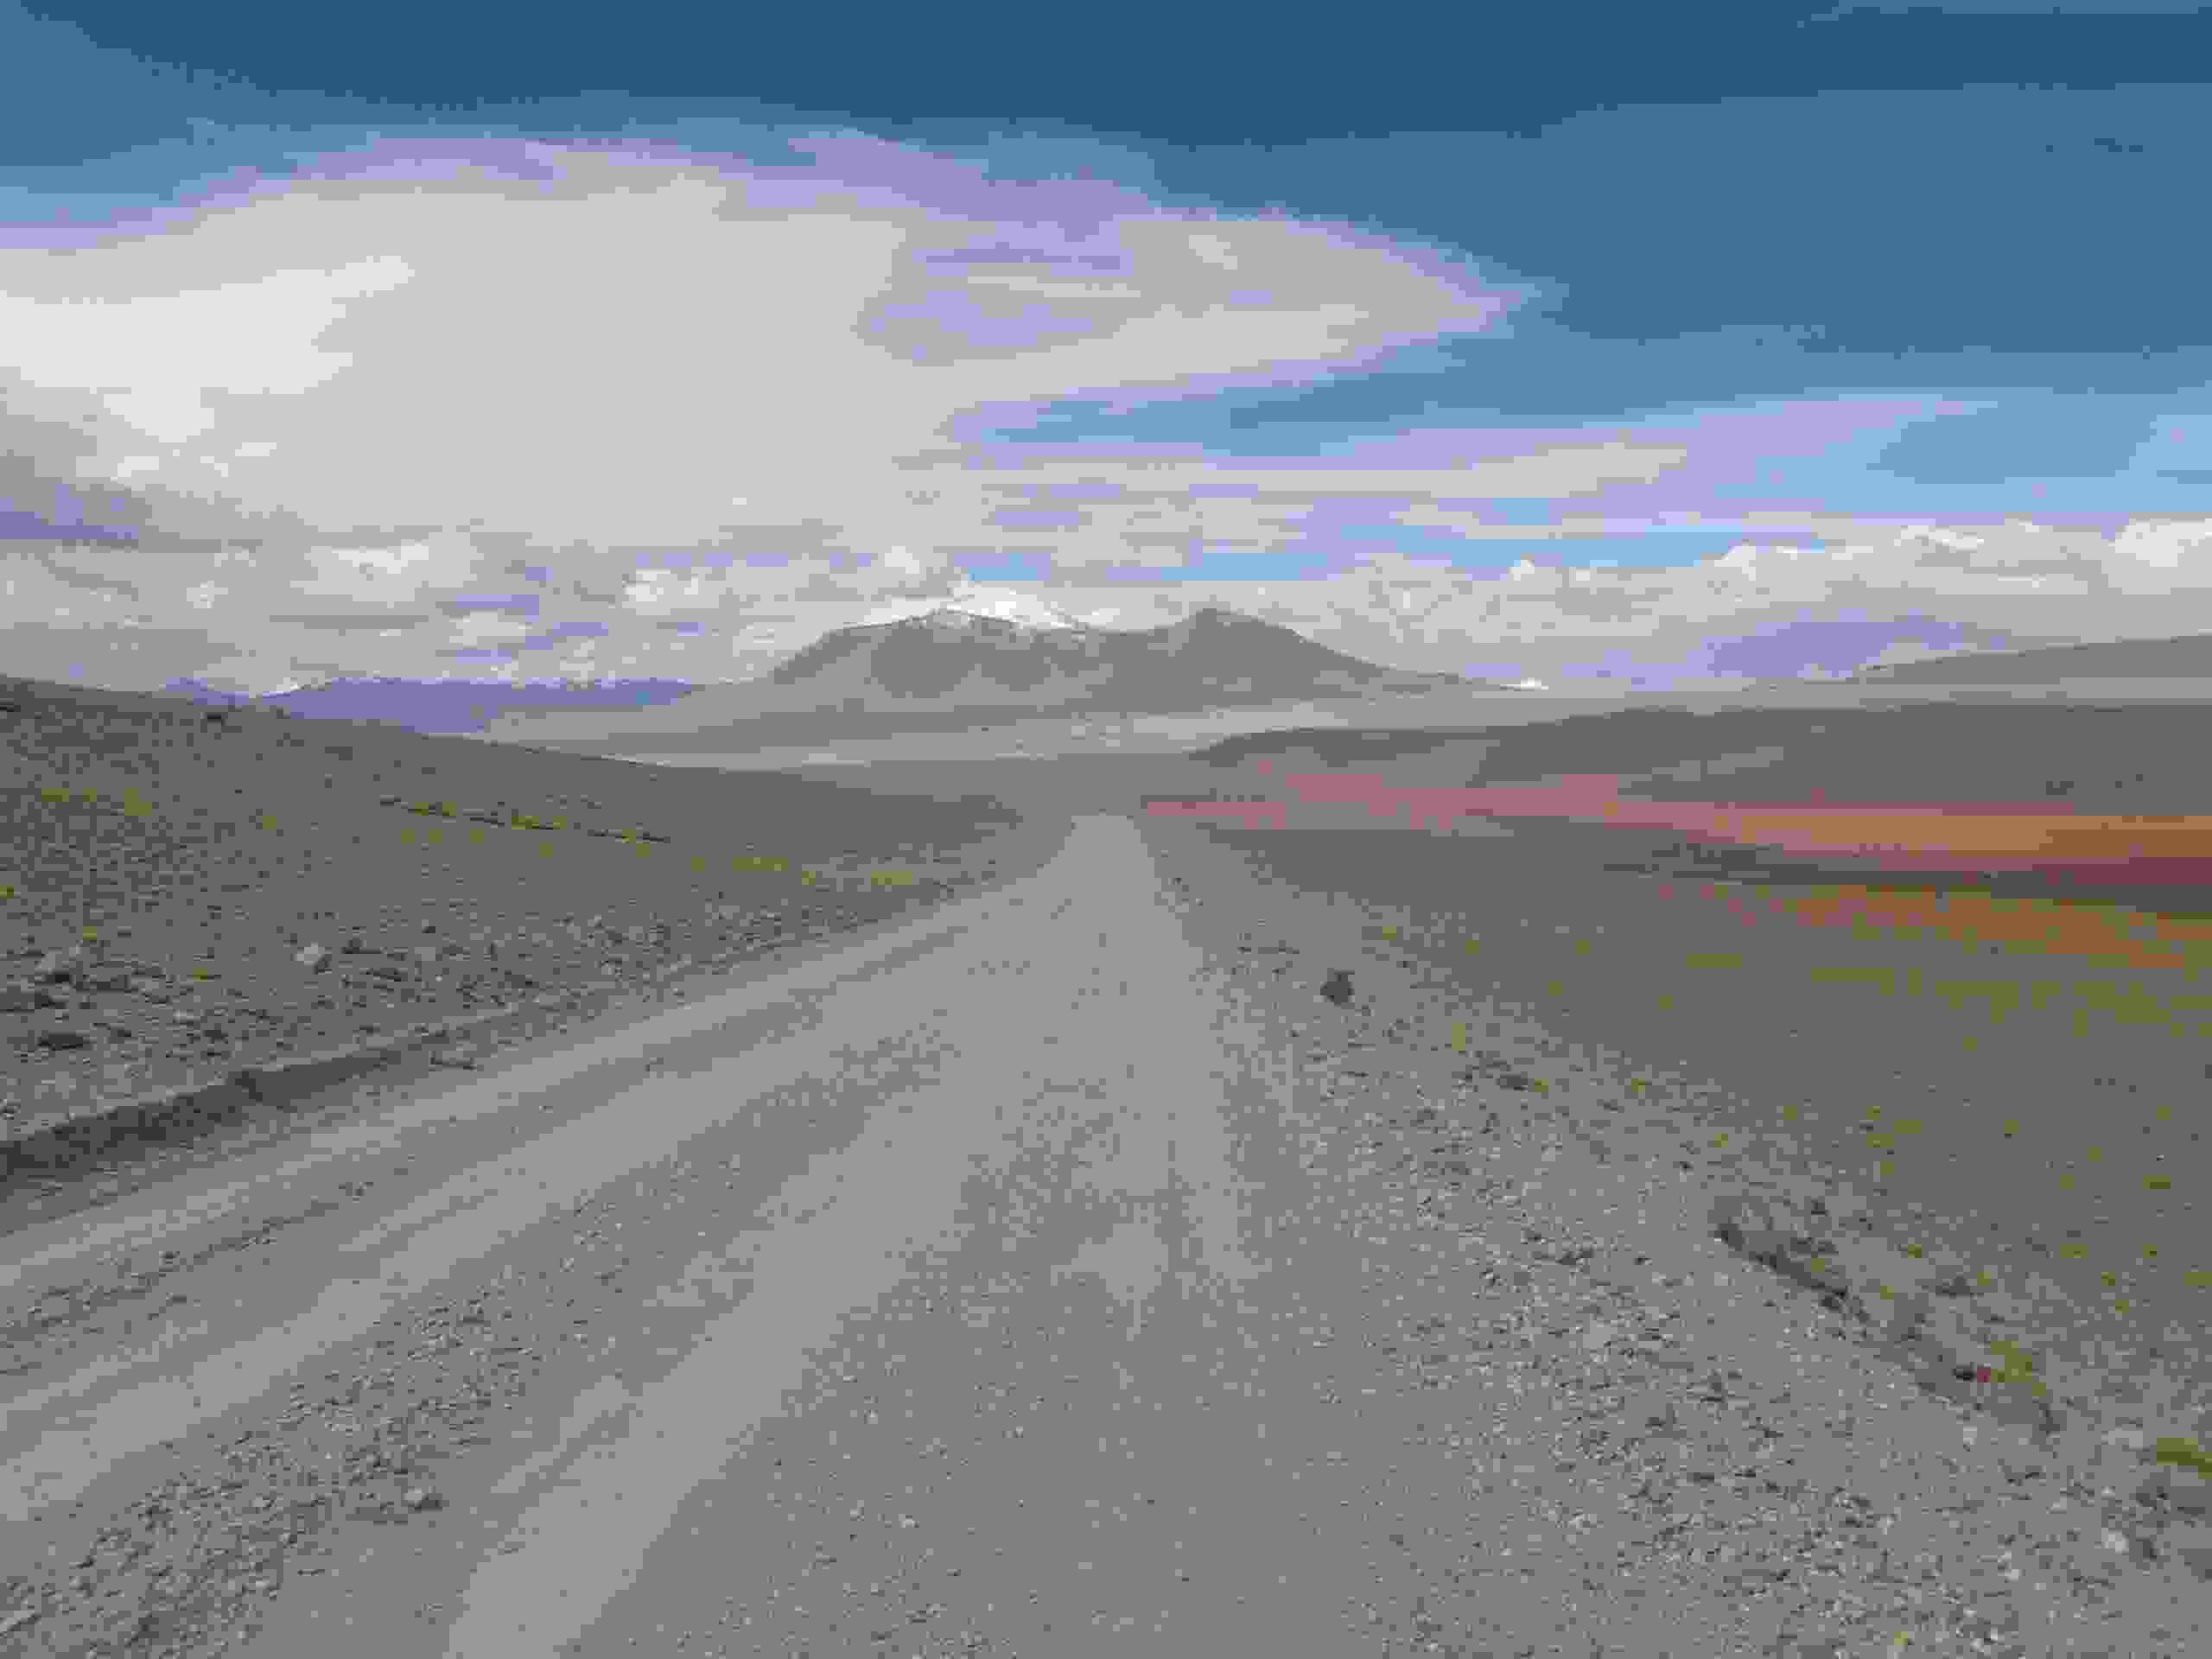
\includegraphics[width=\mywidth]{../wp-content/uploads/2015/04/wpid-wp-1427984180040.jpg} } 
 \newline
 On passe devant le Desierto de Dali. \newline
 \newline
\centerline{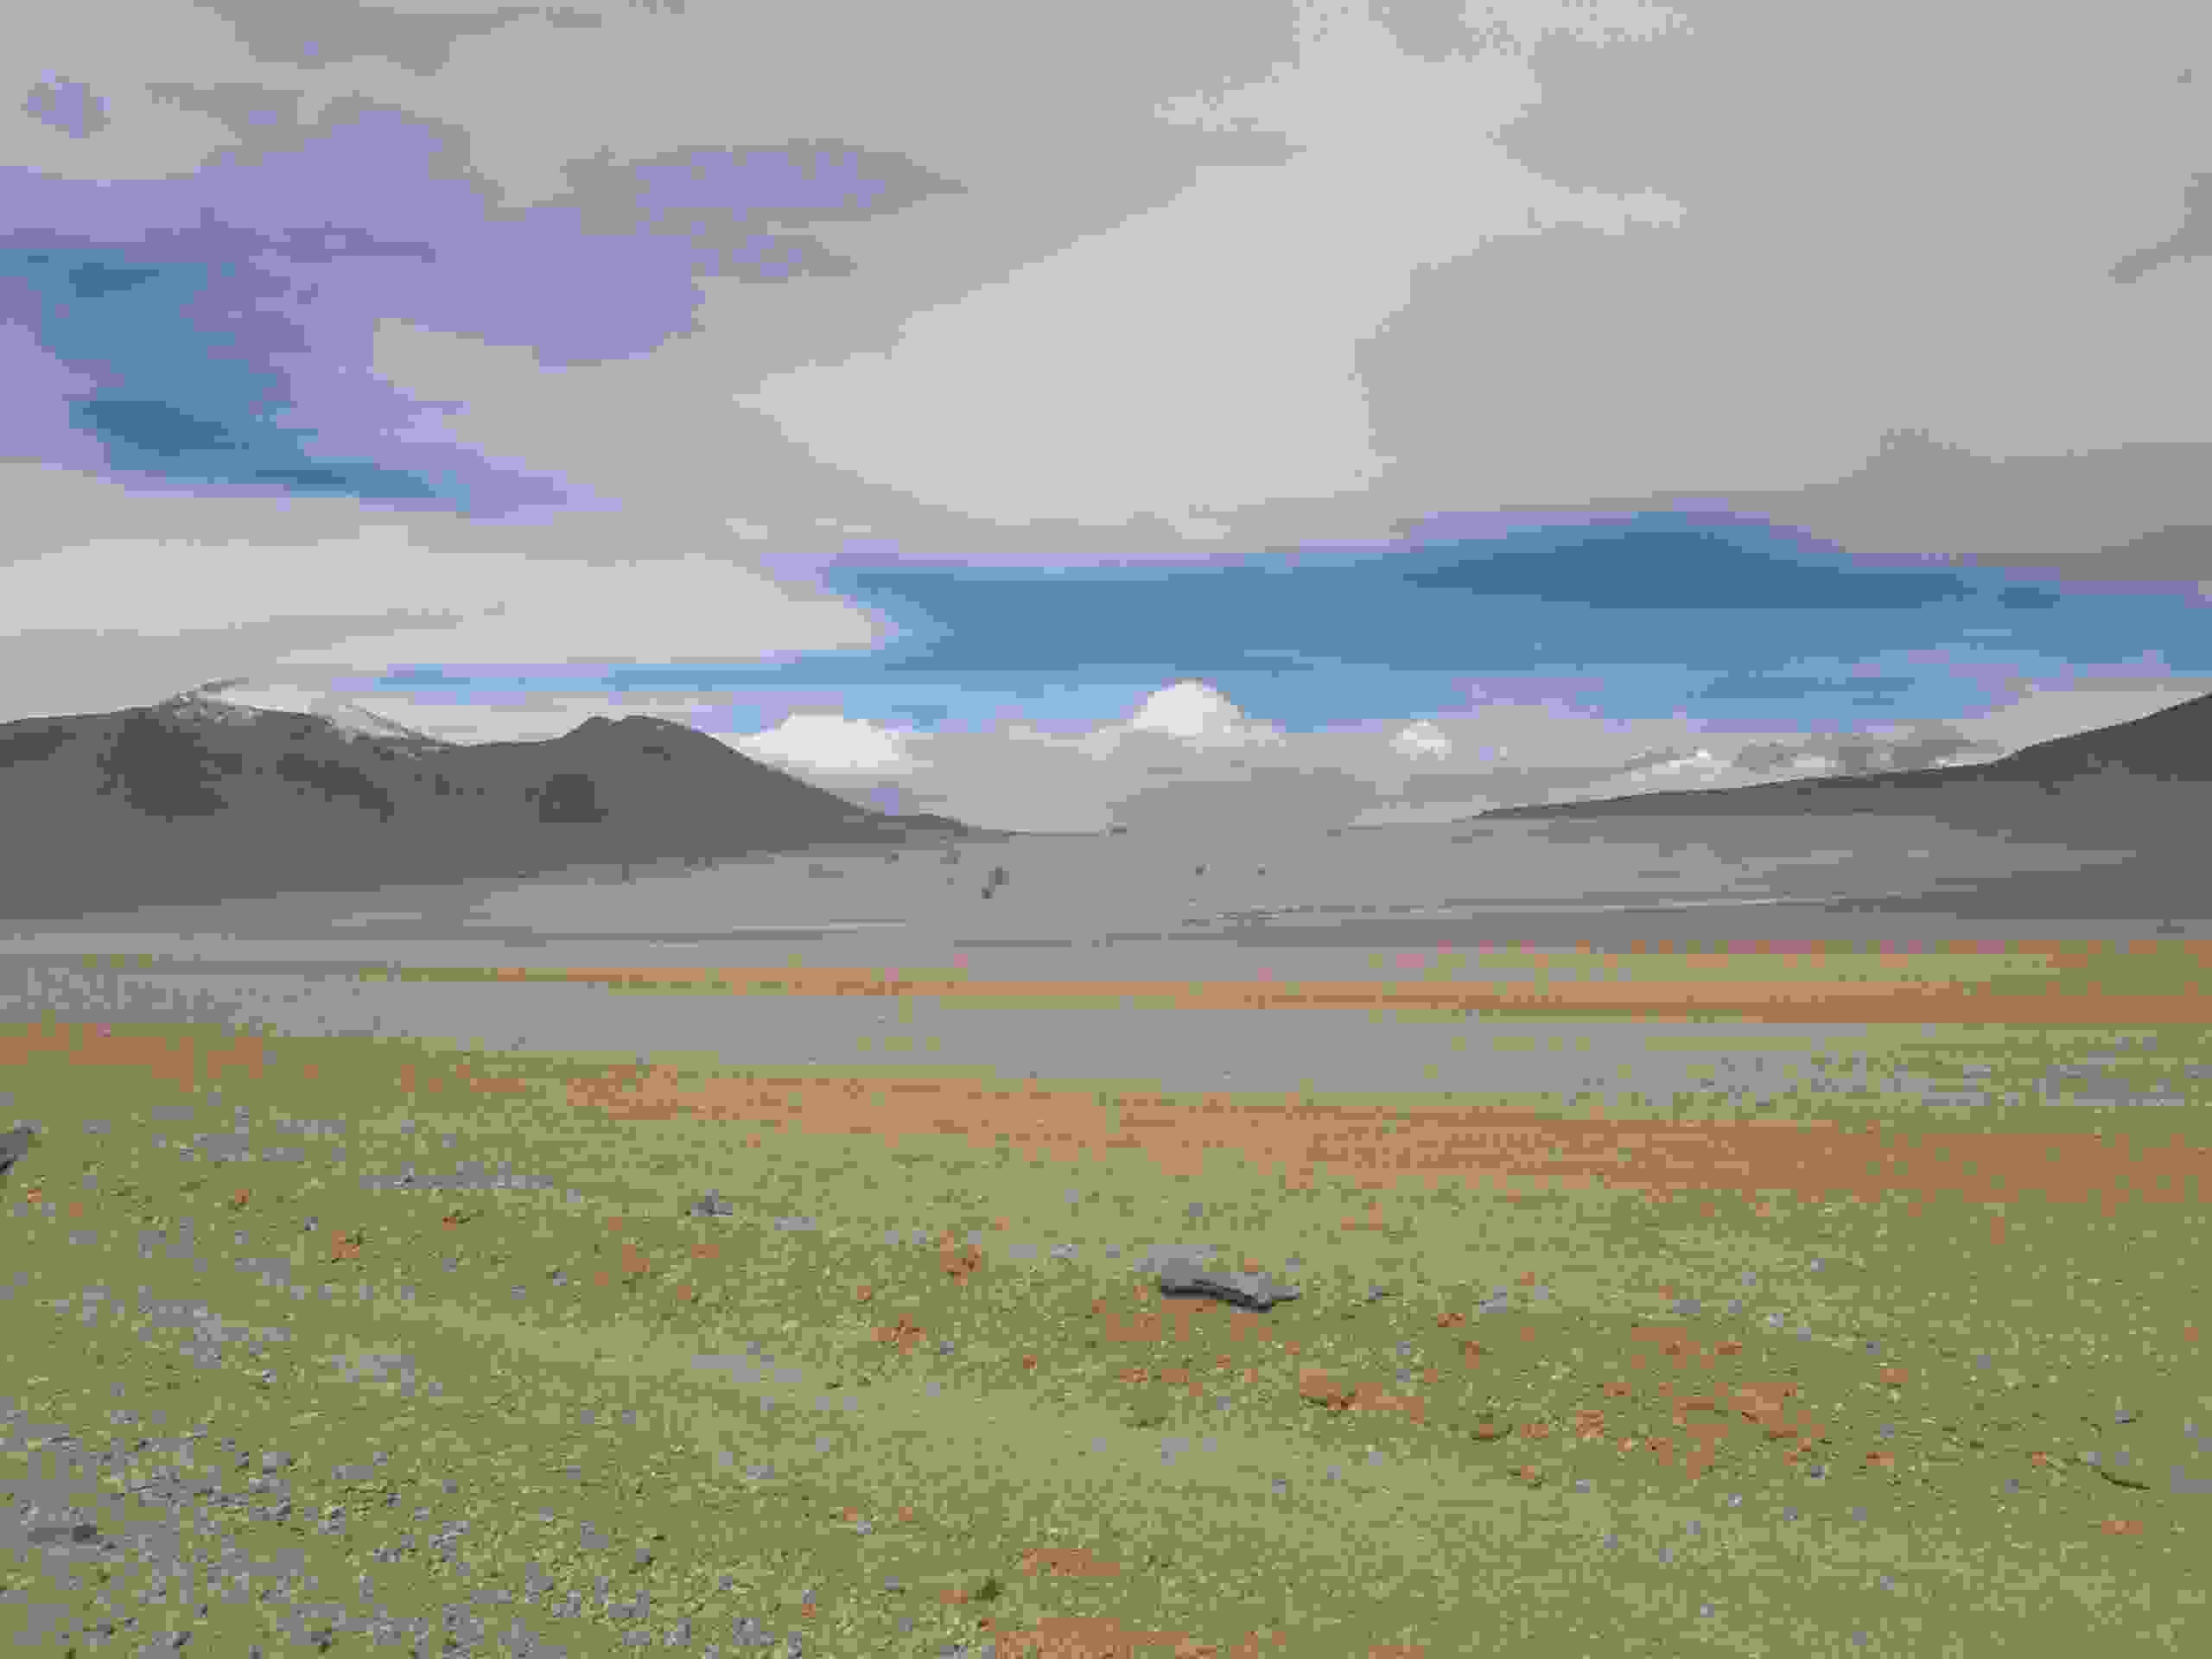
\includegraphics[width=\mywidth]{../wp-content/uploads/2015/04/wpid-wp-1427984489619.jpg} } 
 \newline
 Piscine d'eau chaude devant la Laguna Chalviri pour terminer la journée. \newline
 \newline
\centerline{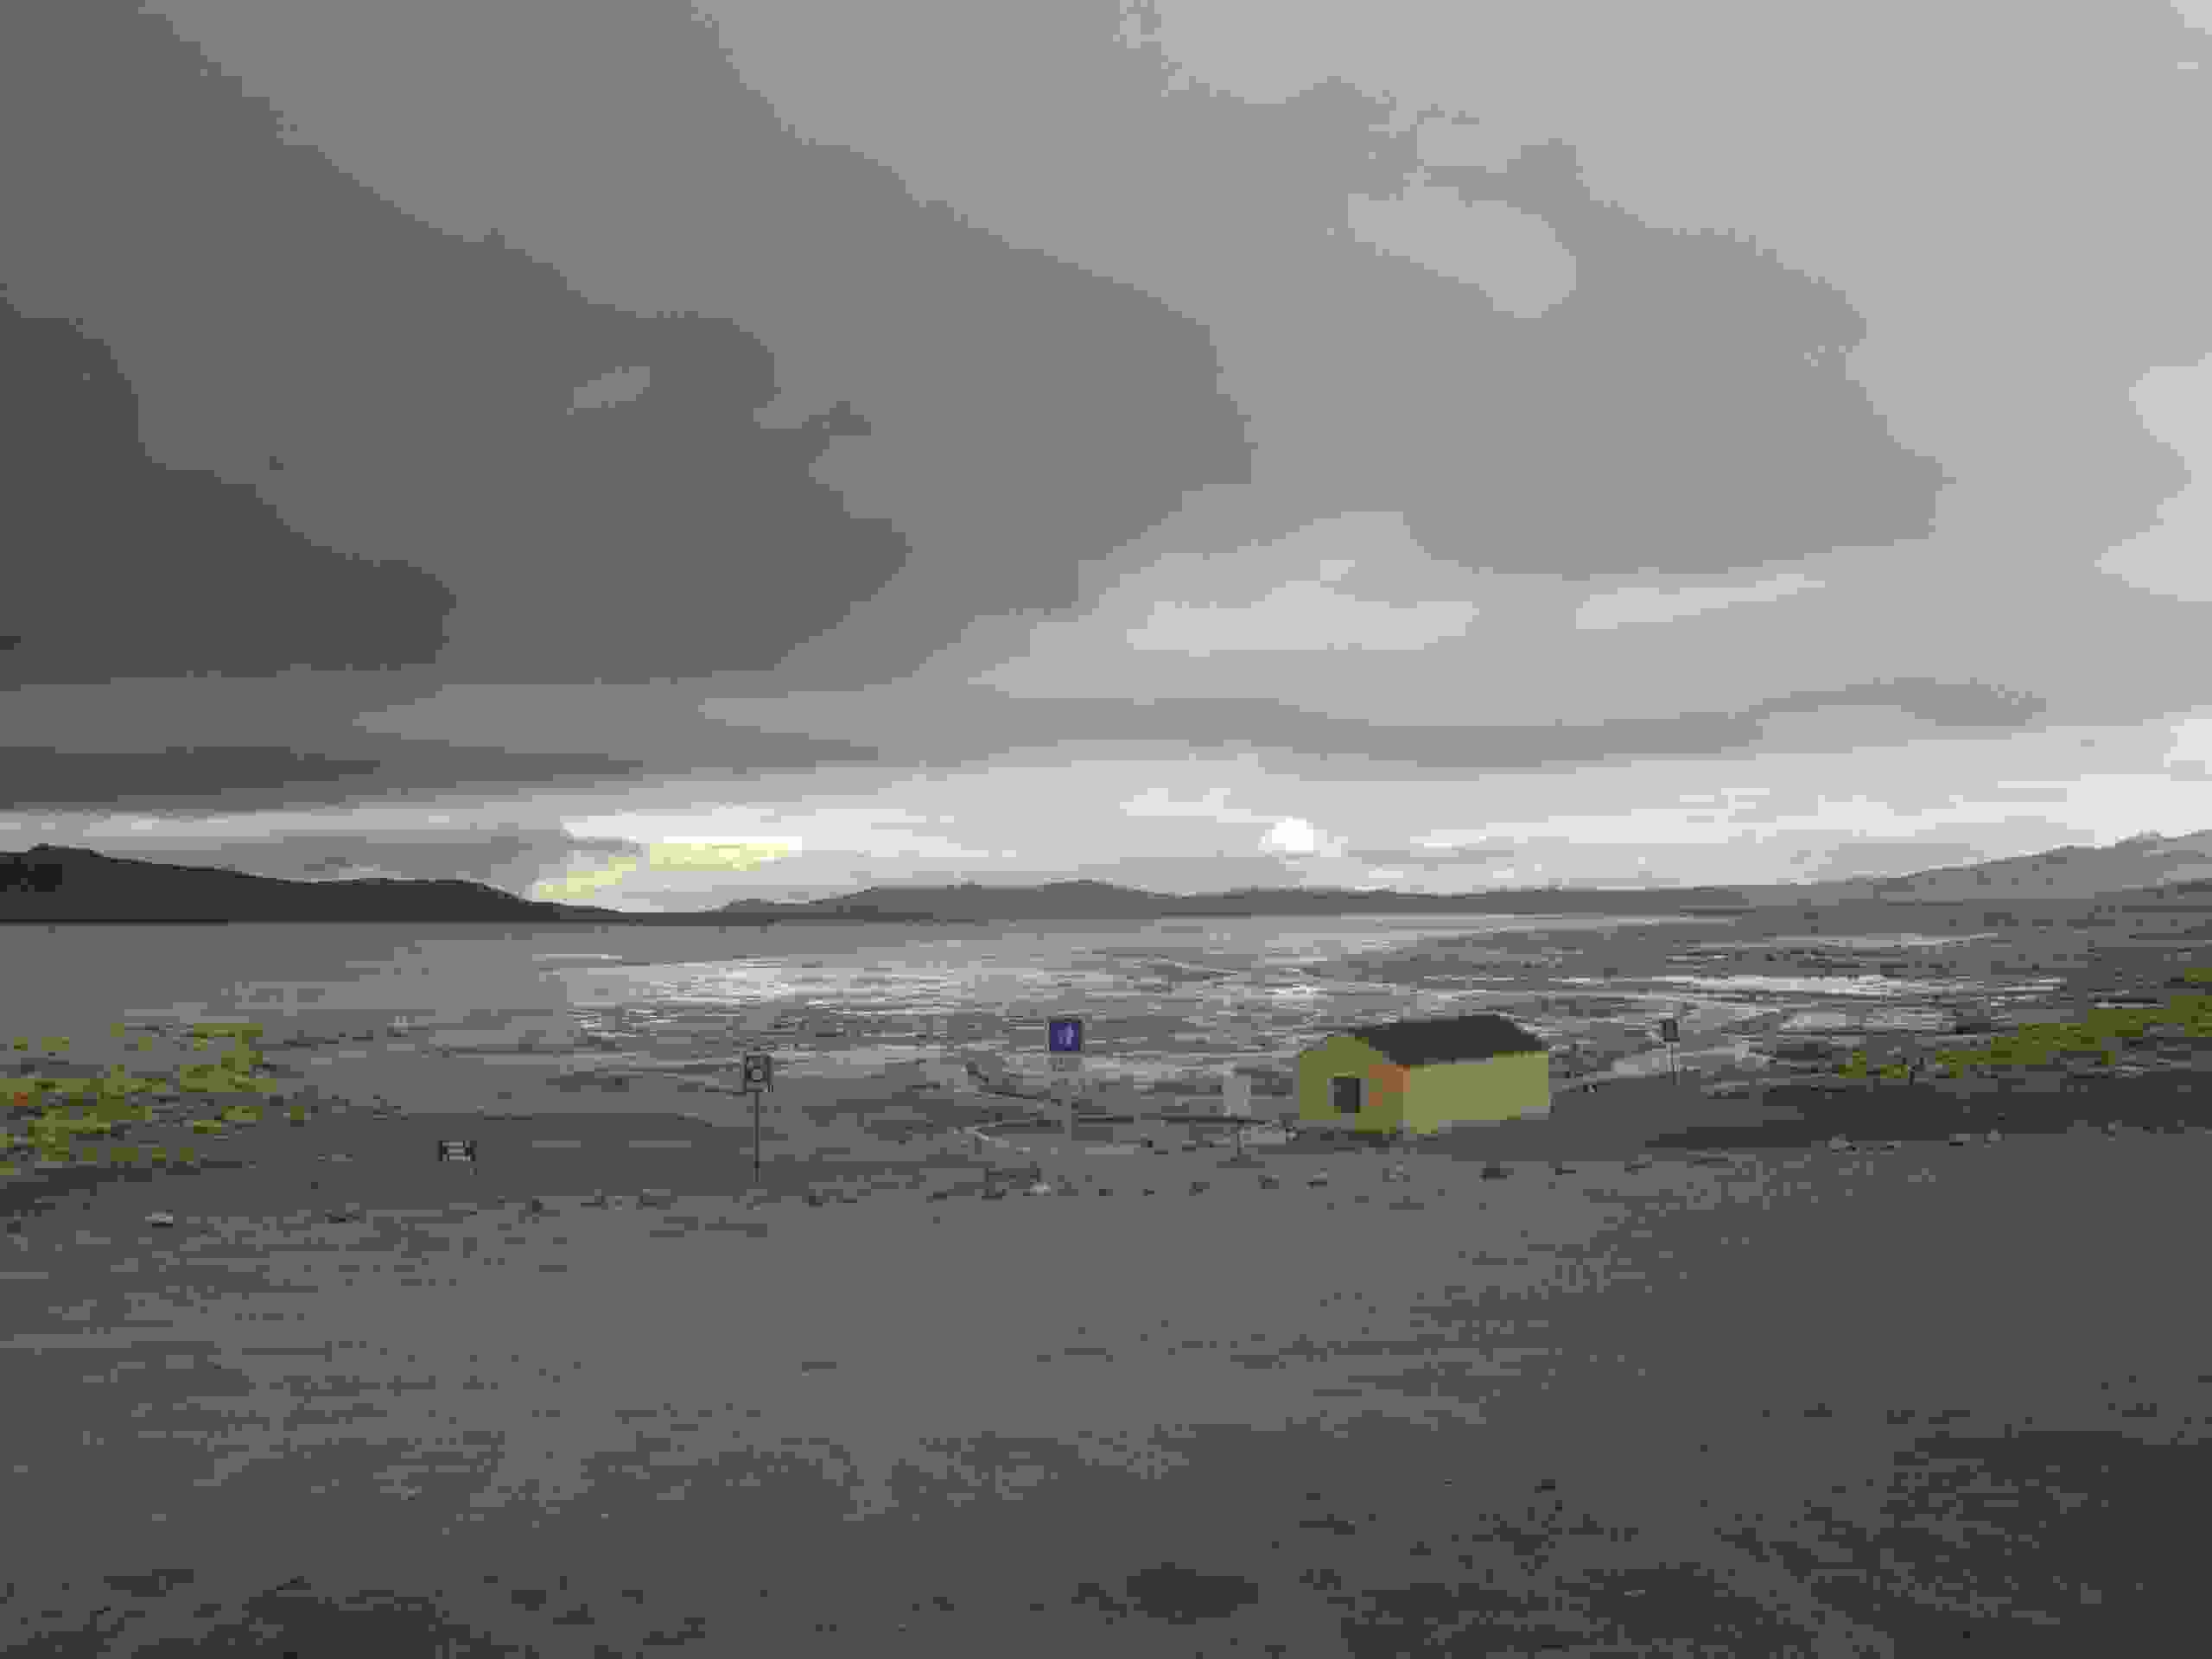
\includegraphics[width=\mywidth]{../wp-content/uploads/2015/04/wpid-wp-1427984540238.jpg} } 
 \newline
 \newline
\centerline{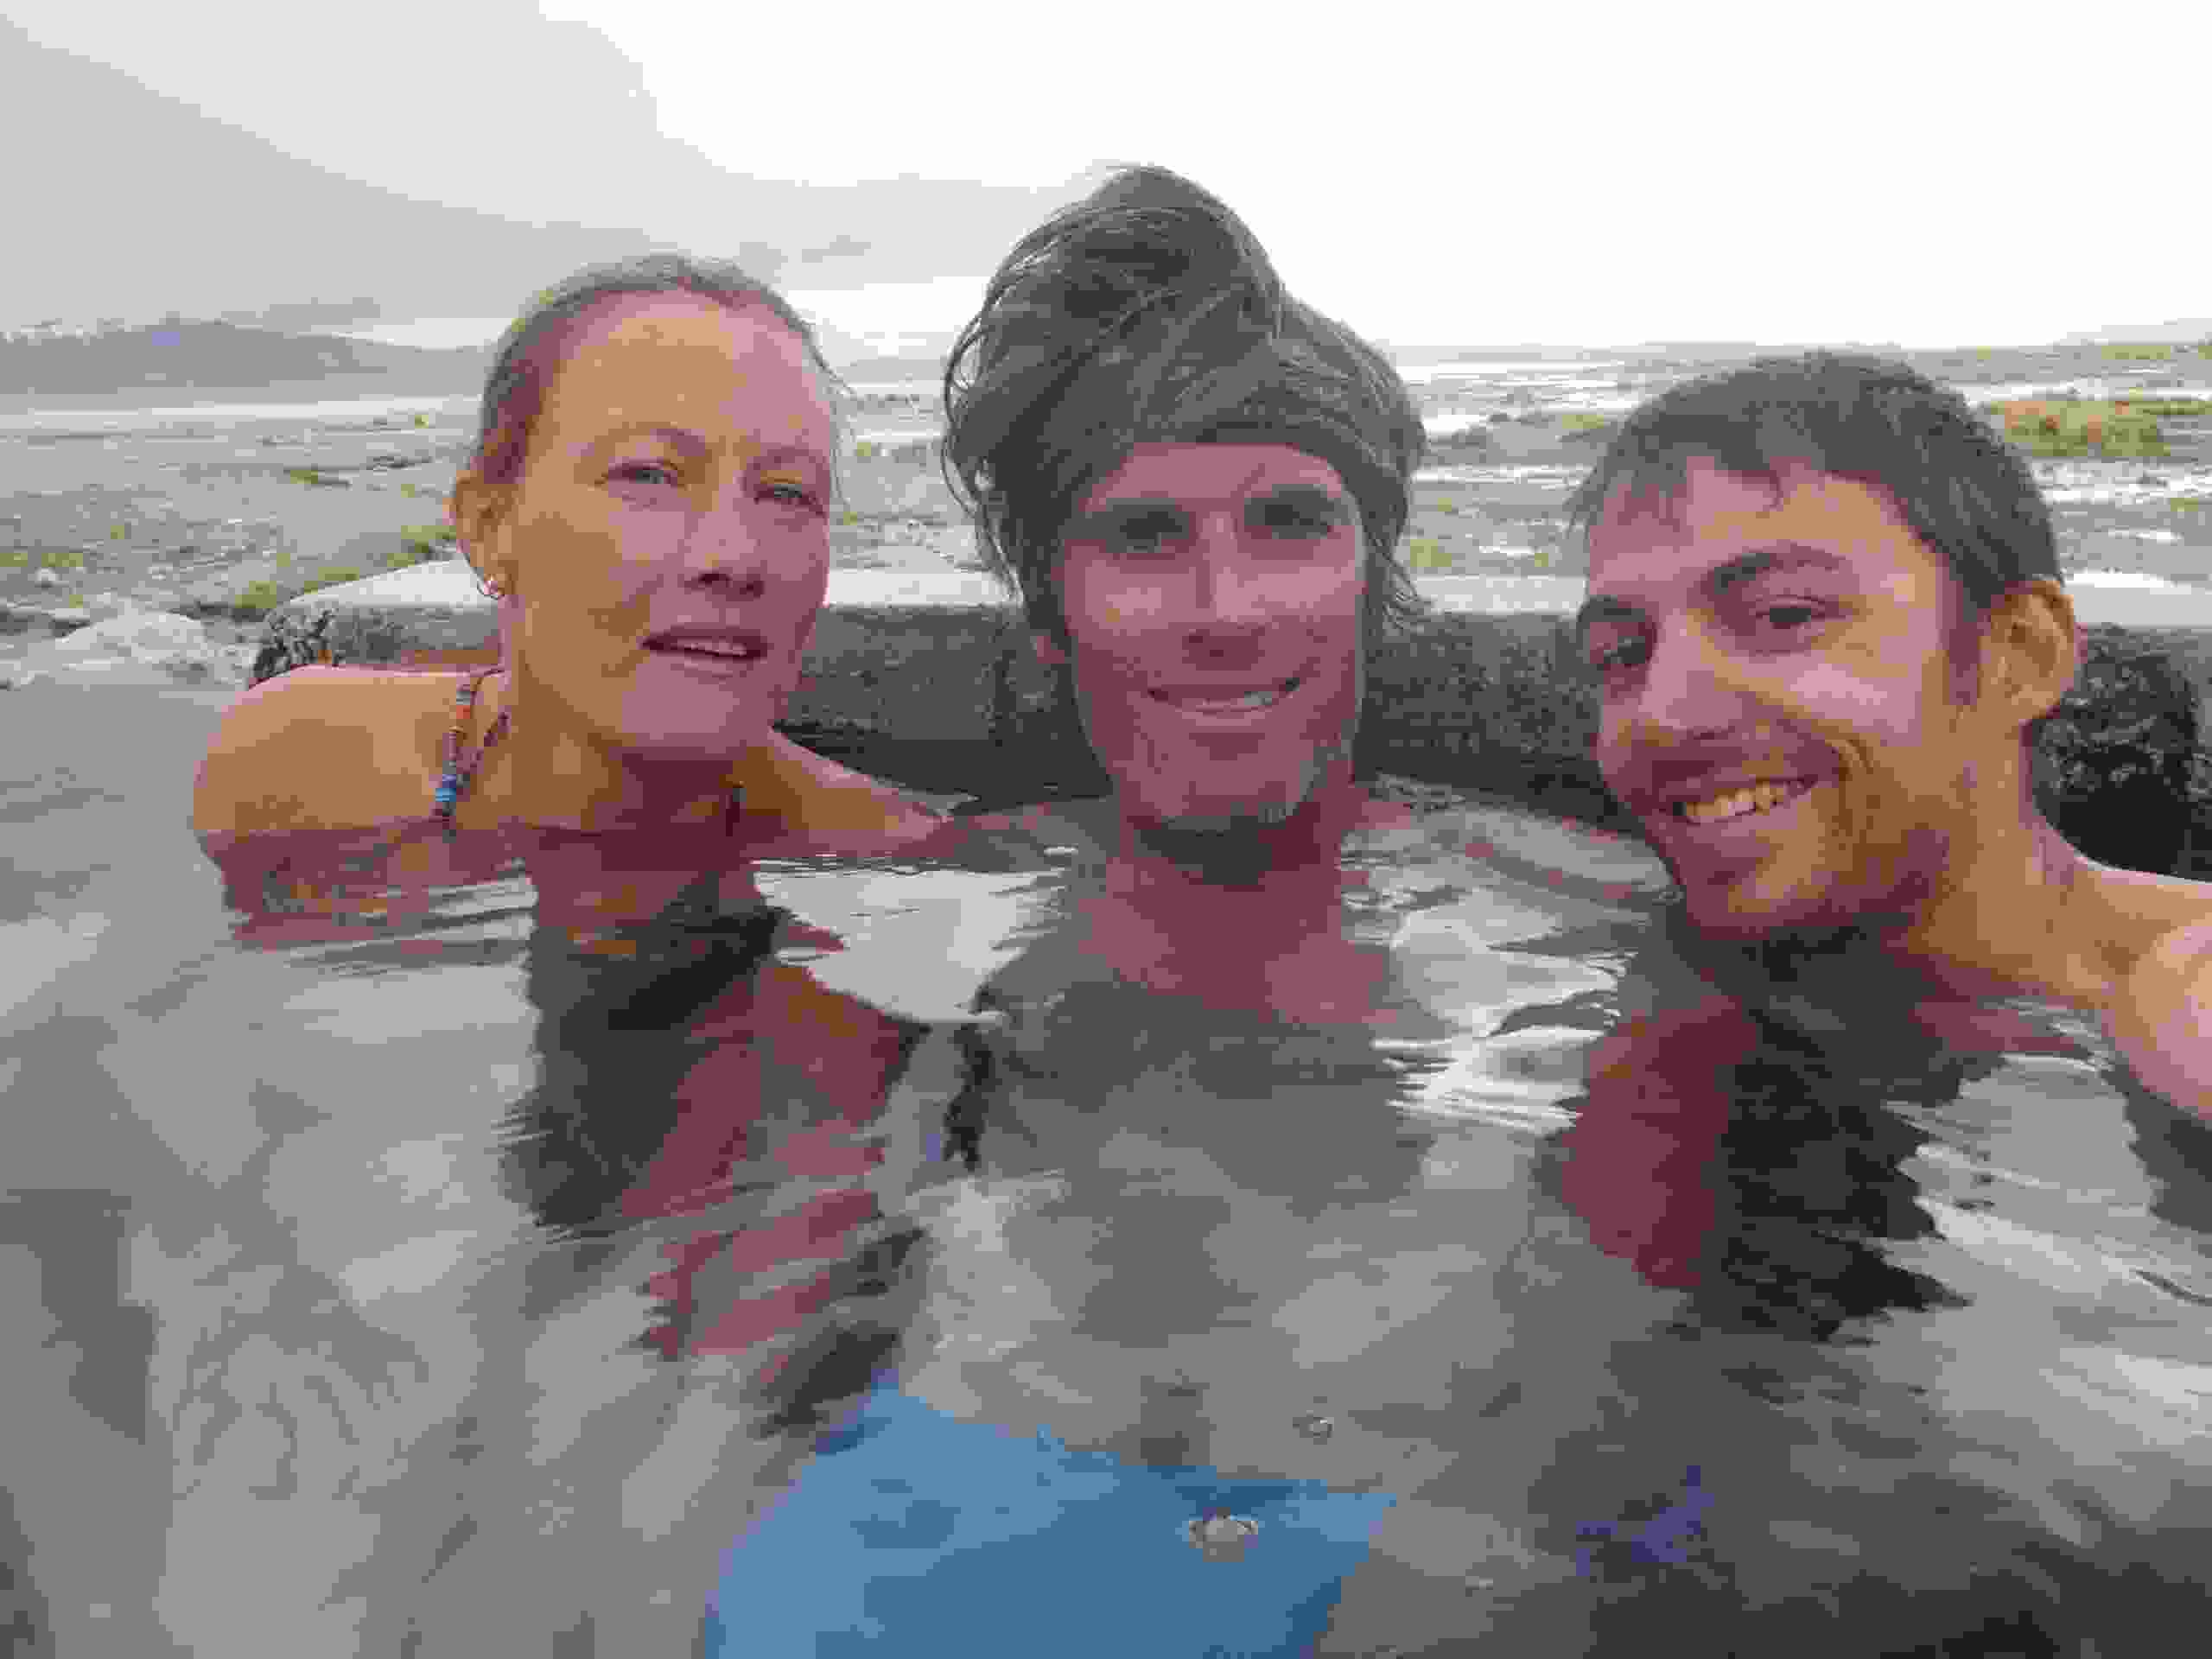
\includegraphics[width=\mywidth]{../wp-content/uploads/2015/04/wpid-wp-1427984554621.jpg} } 
 \newline
 On passe la nuit dans la salle à manger d'un restaurant. \newline
 \newline
\centerline{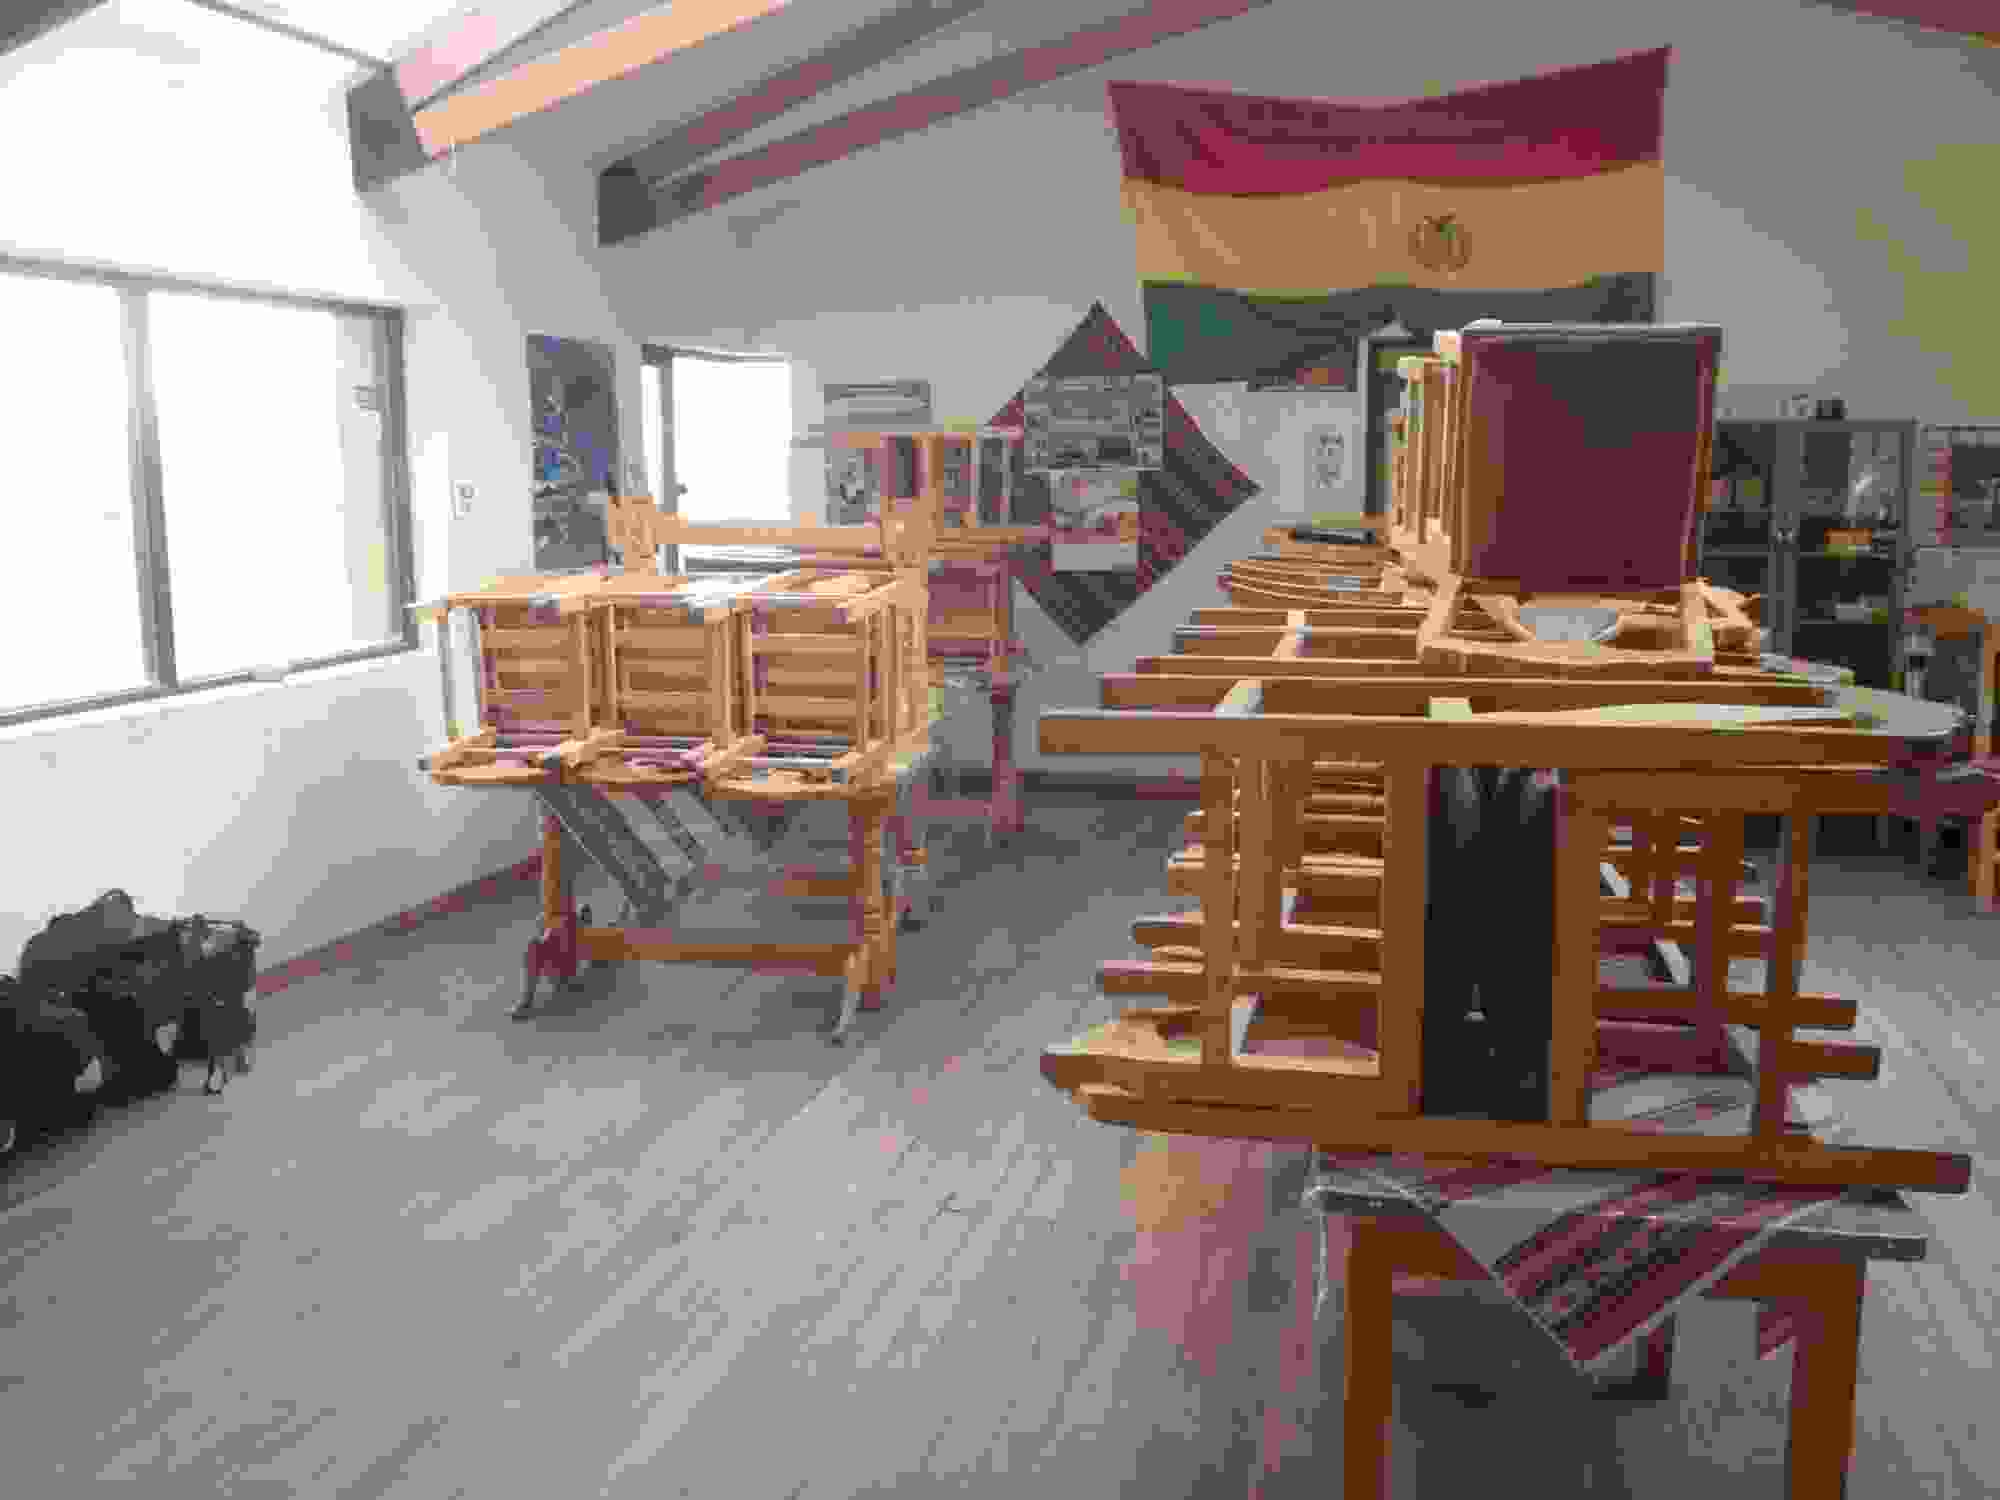
\includegraphics[width=\mywidth]{../wp-content/uploads/2015/04/wpid-wp-1427988917183.jpg} } 
 \newline
 3e jour : \newline
 Lever à 6h pour laisser la place aux touristes en jeep pour le petit déjeuner. \newline
 \newline
\centerline{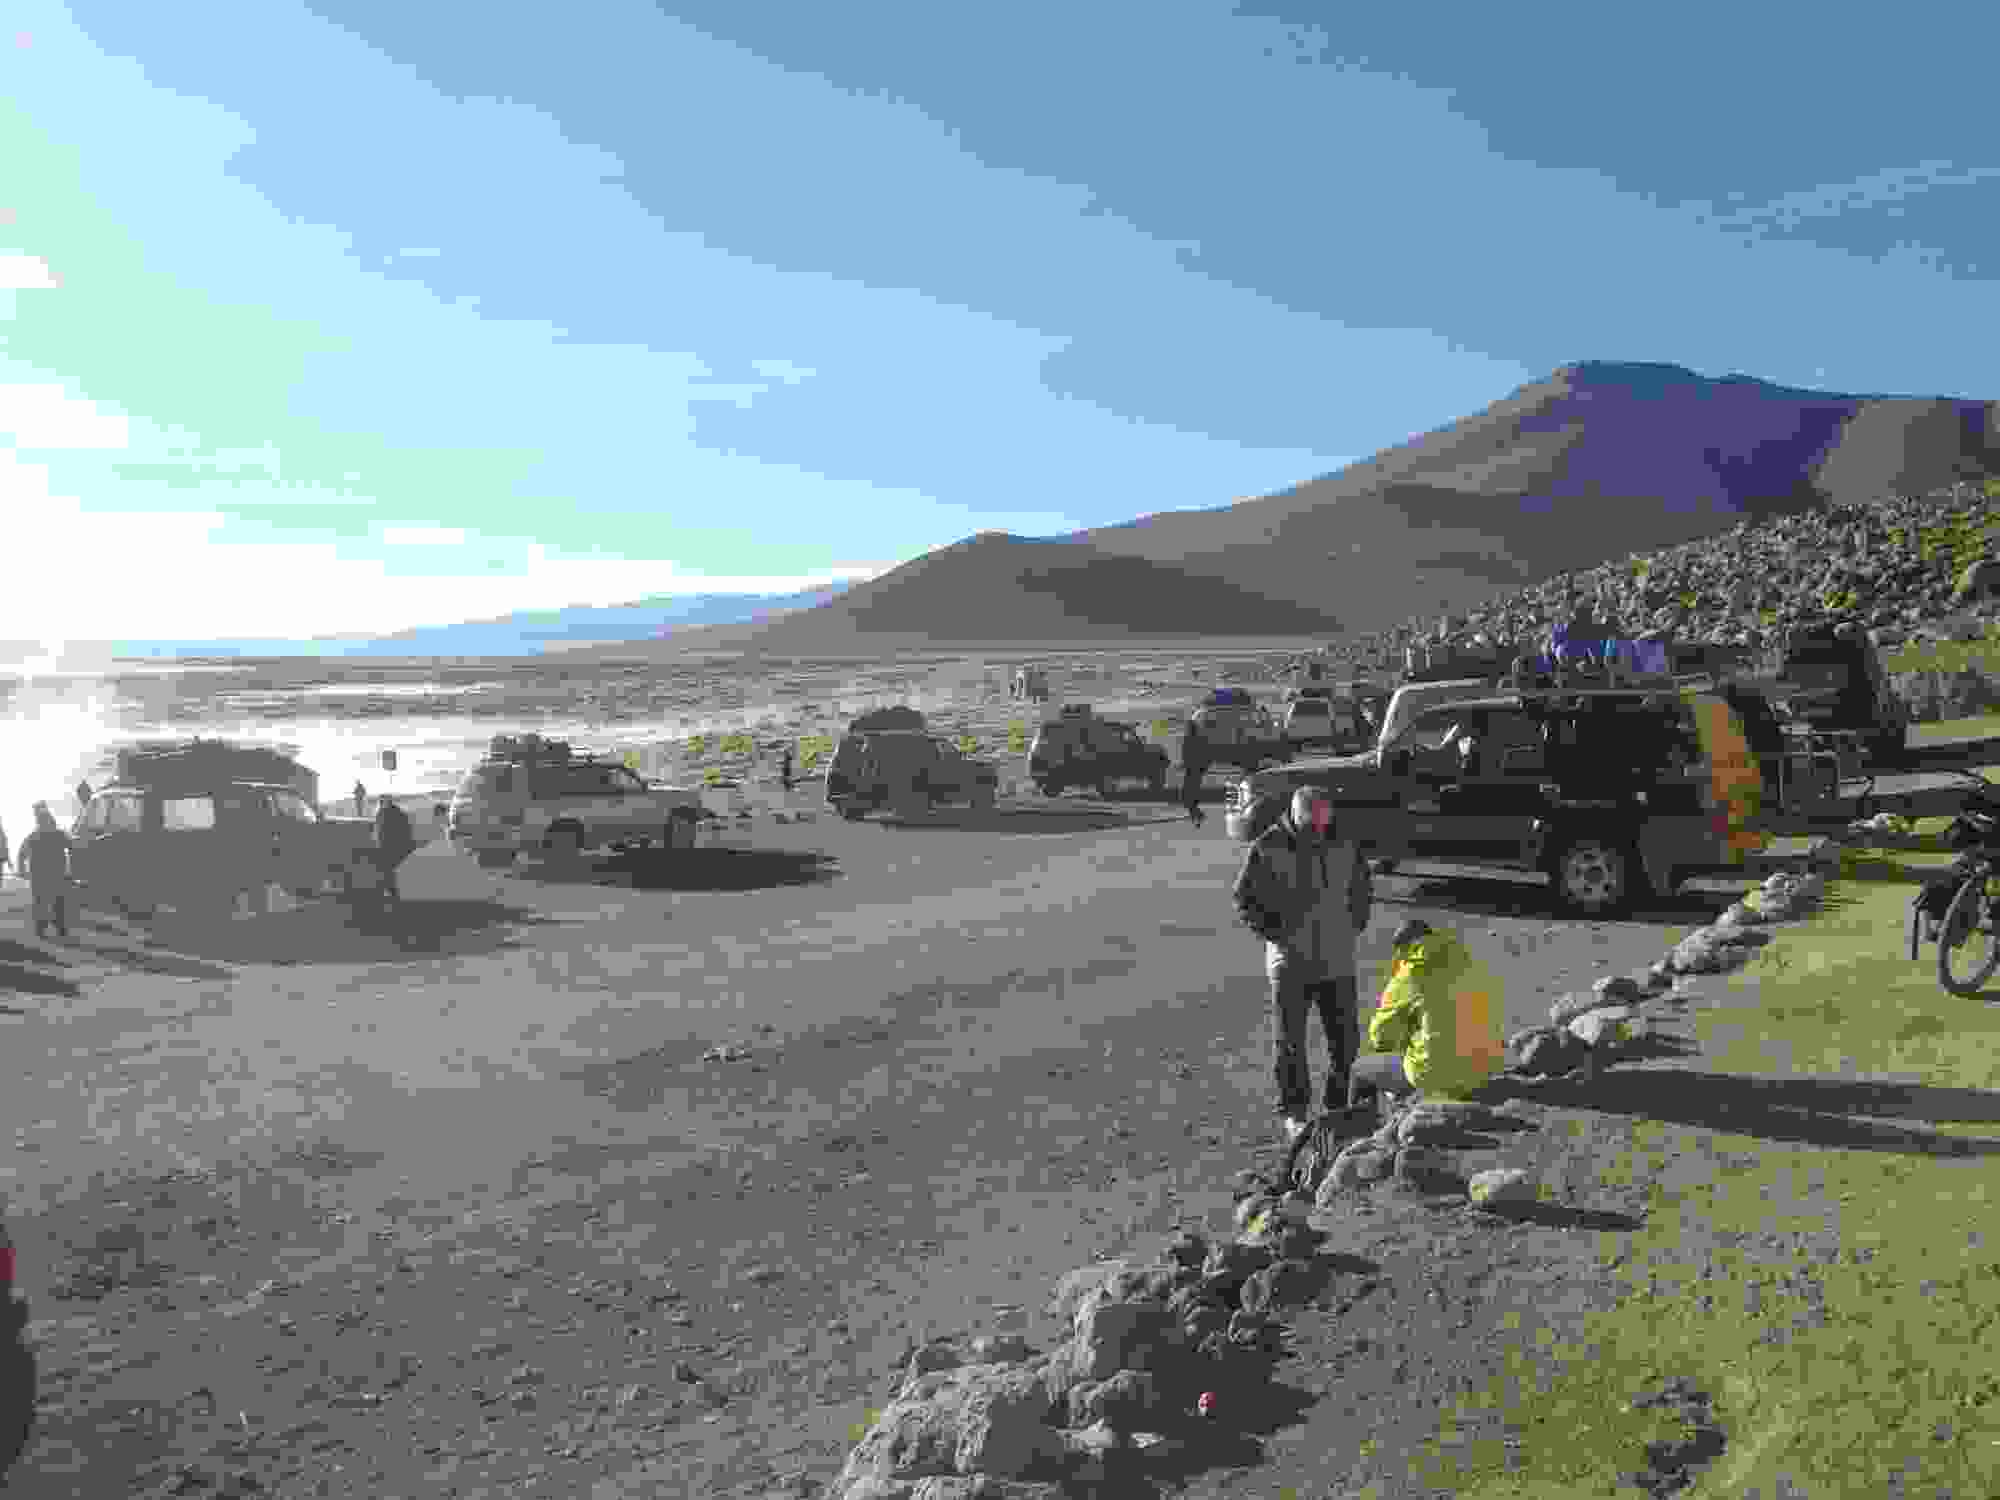
\includegraphics[width=\mywidth]{../wp-content/uploads/2015/04/wpid-wp-1427987293614.jpg} } 
 \newline
 20km de belle montée. \newline
 \newline
\centerline{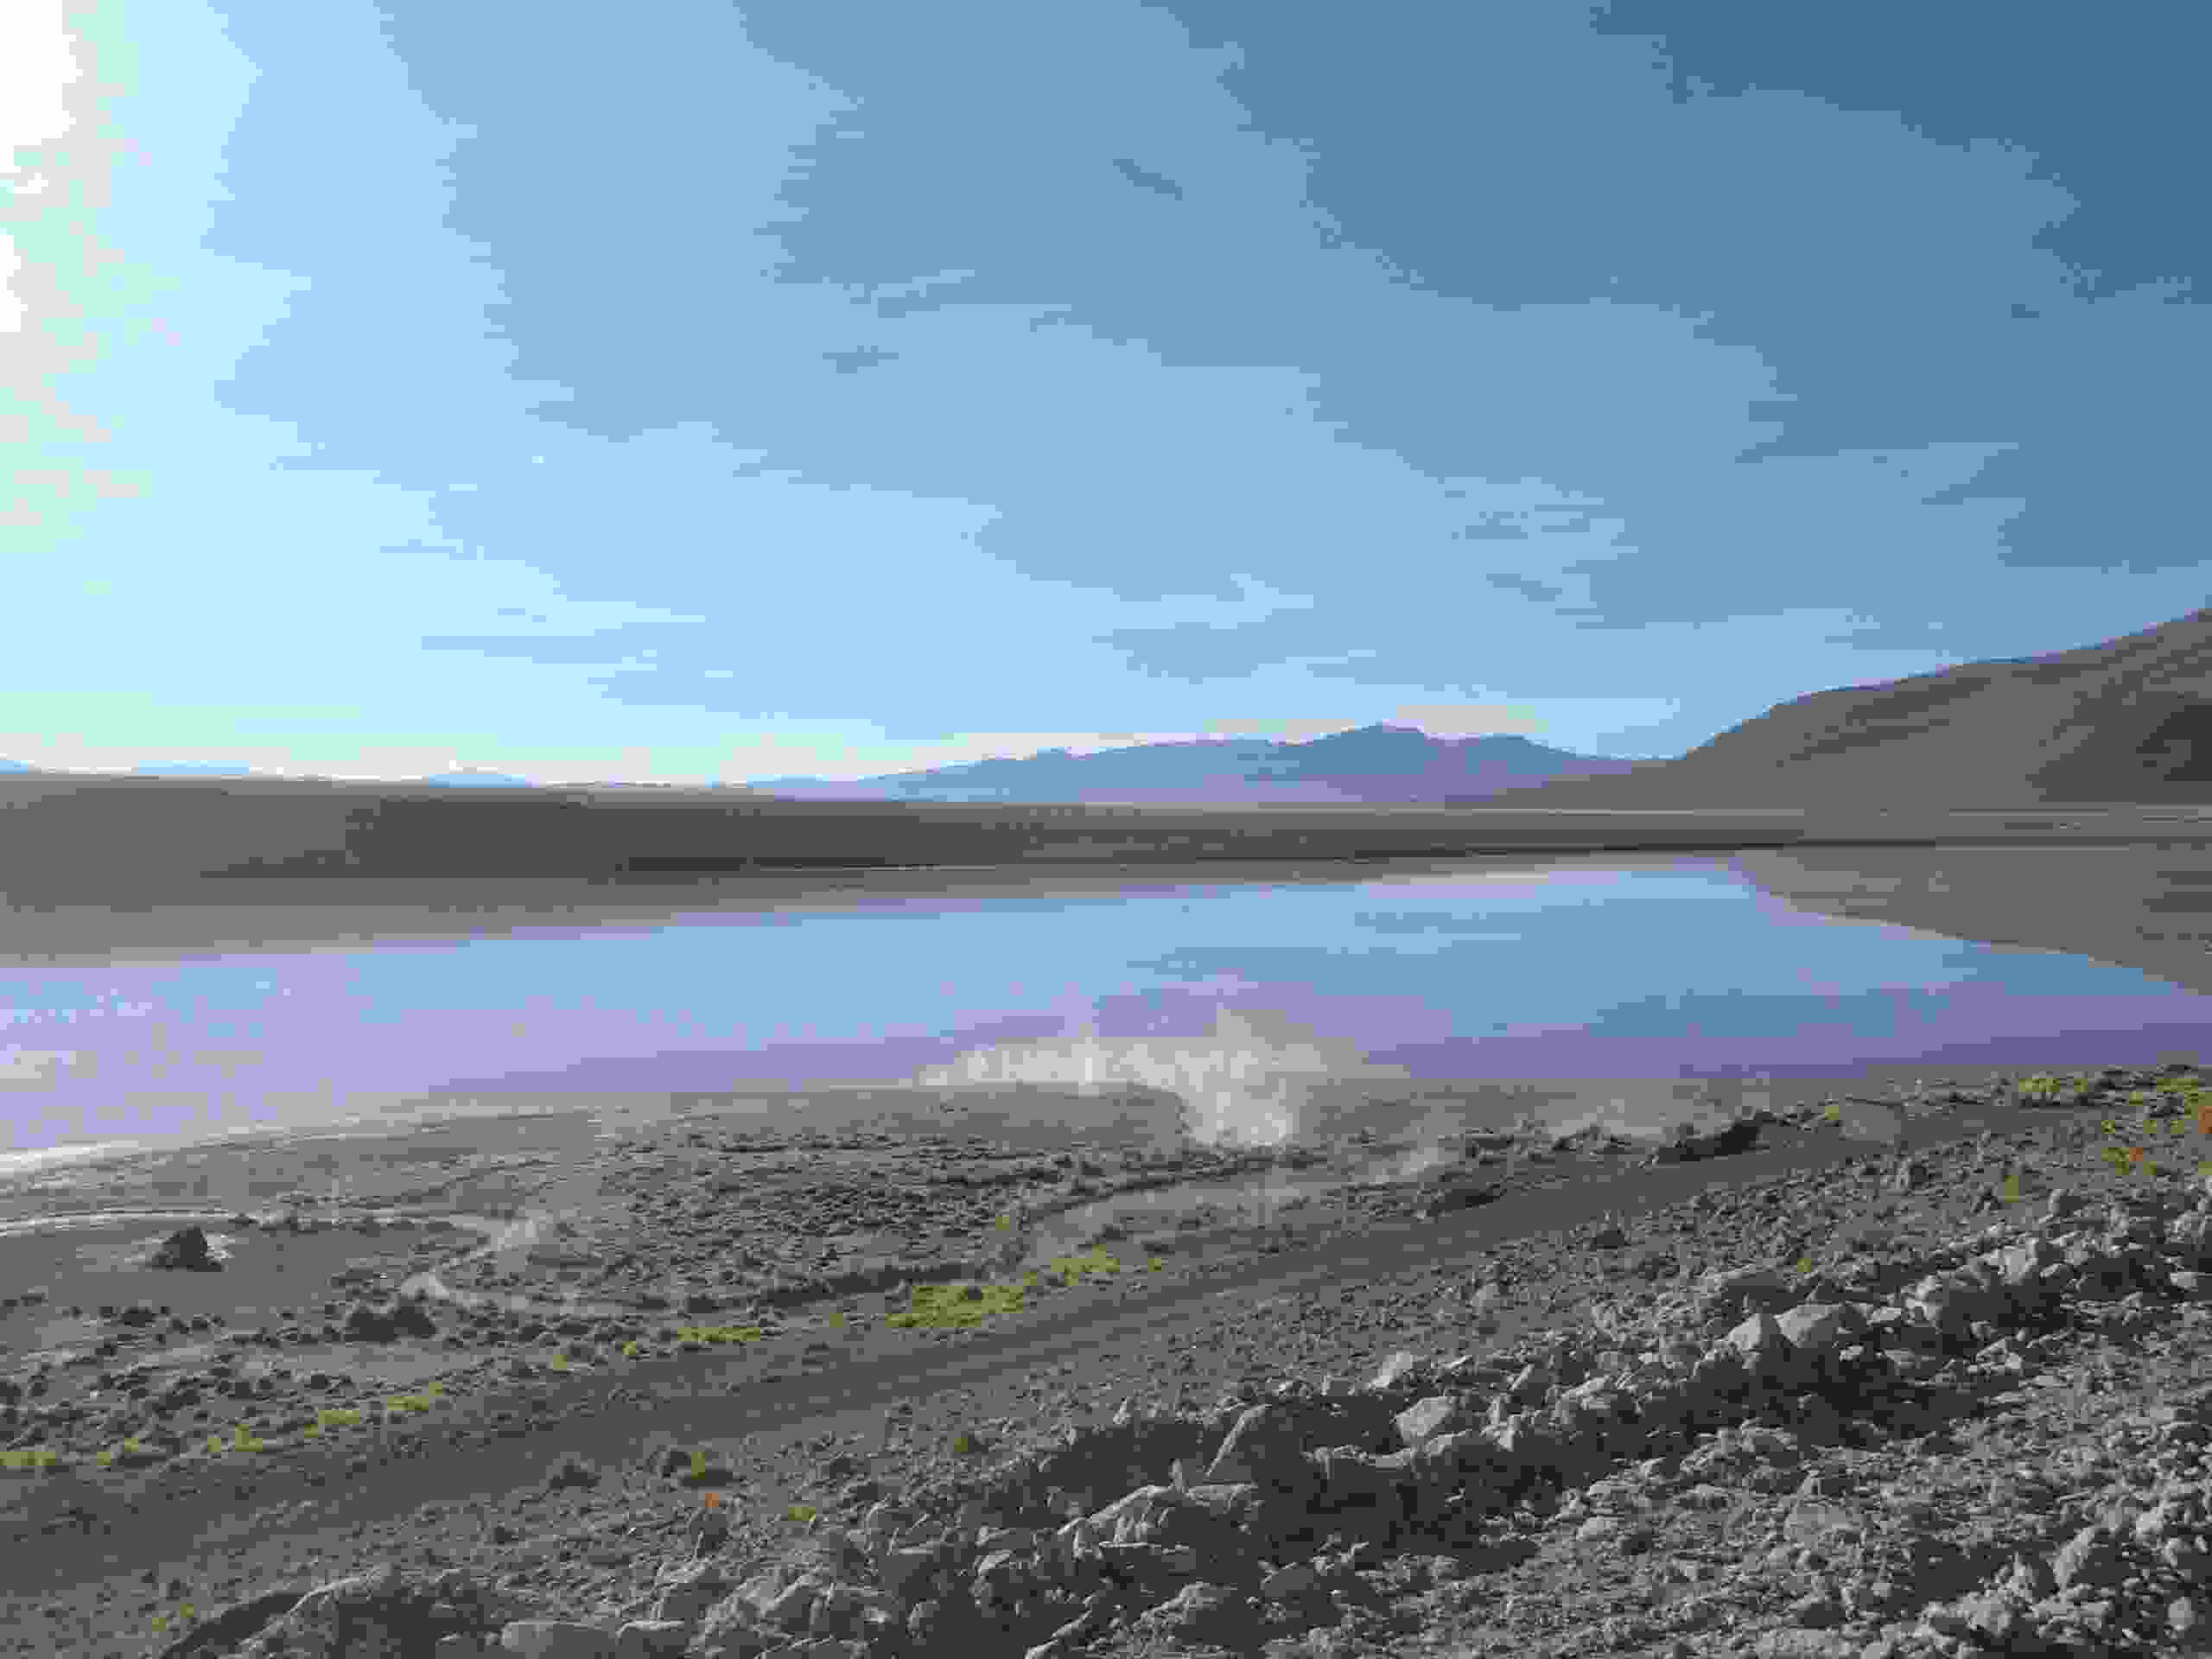
\includegraphics[width=\mywidth]{../wp-content/uploads/2015/04/wpid-wp-1427984607804.jpg} } 
 \newline
 \newline
\centerline{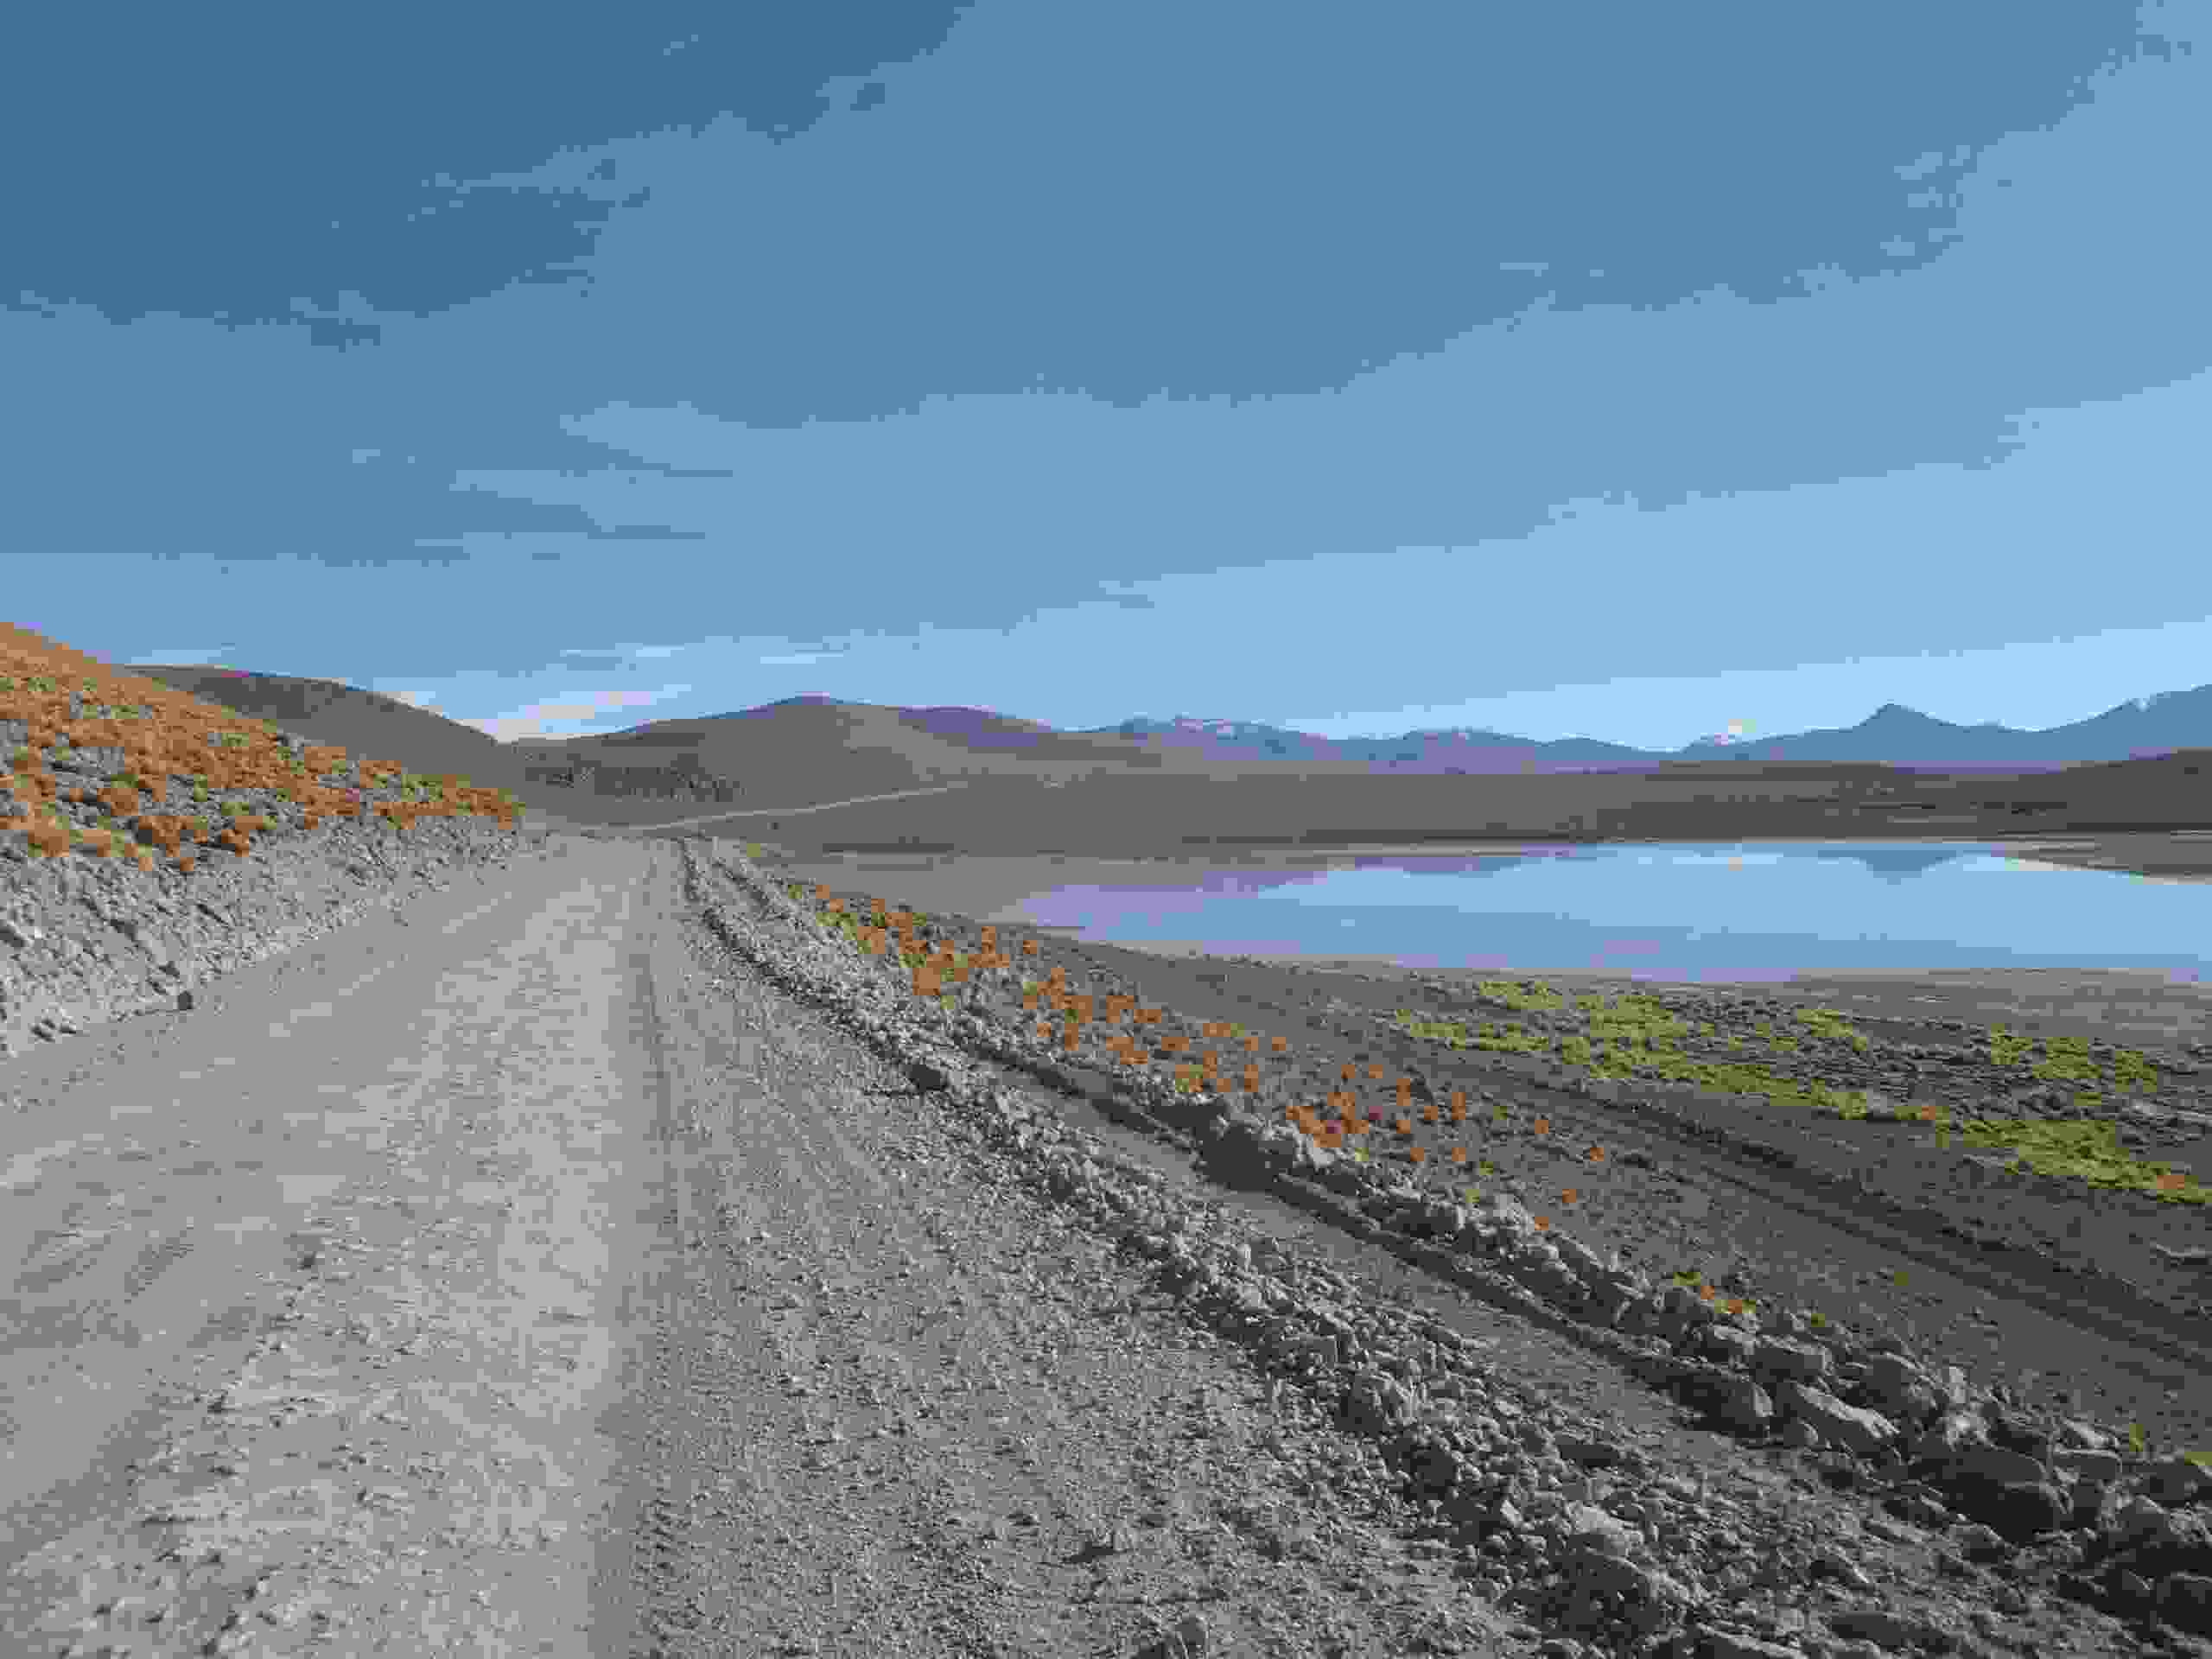
\includegraphics[width=\mywidth]{../wp-content/uploads/2015/04/wpid-wp-1427984674366.jpg} } 
 \newline
 \newline
\centerline{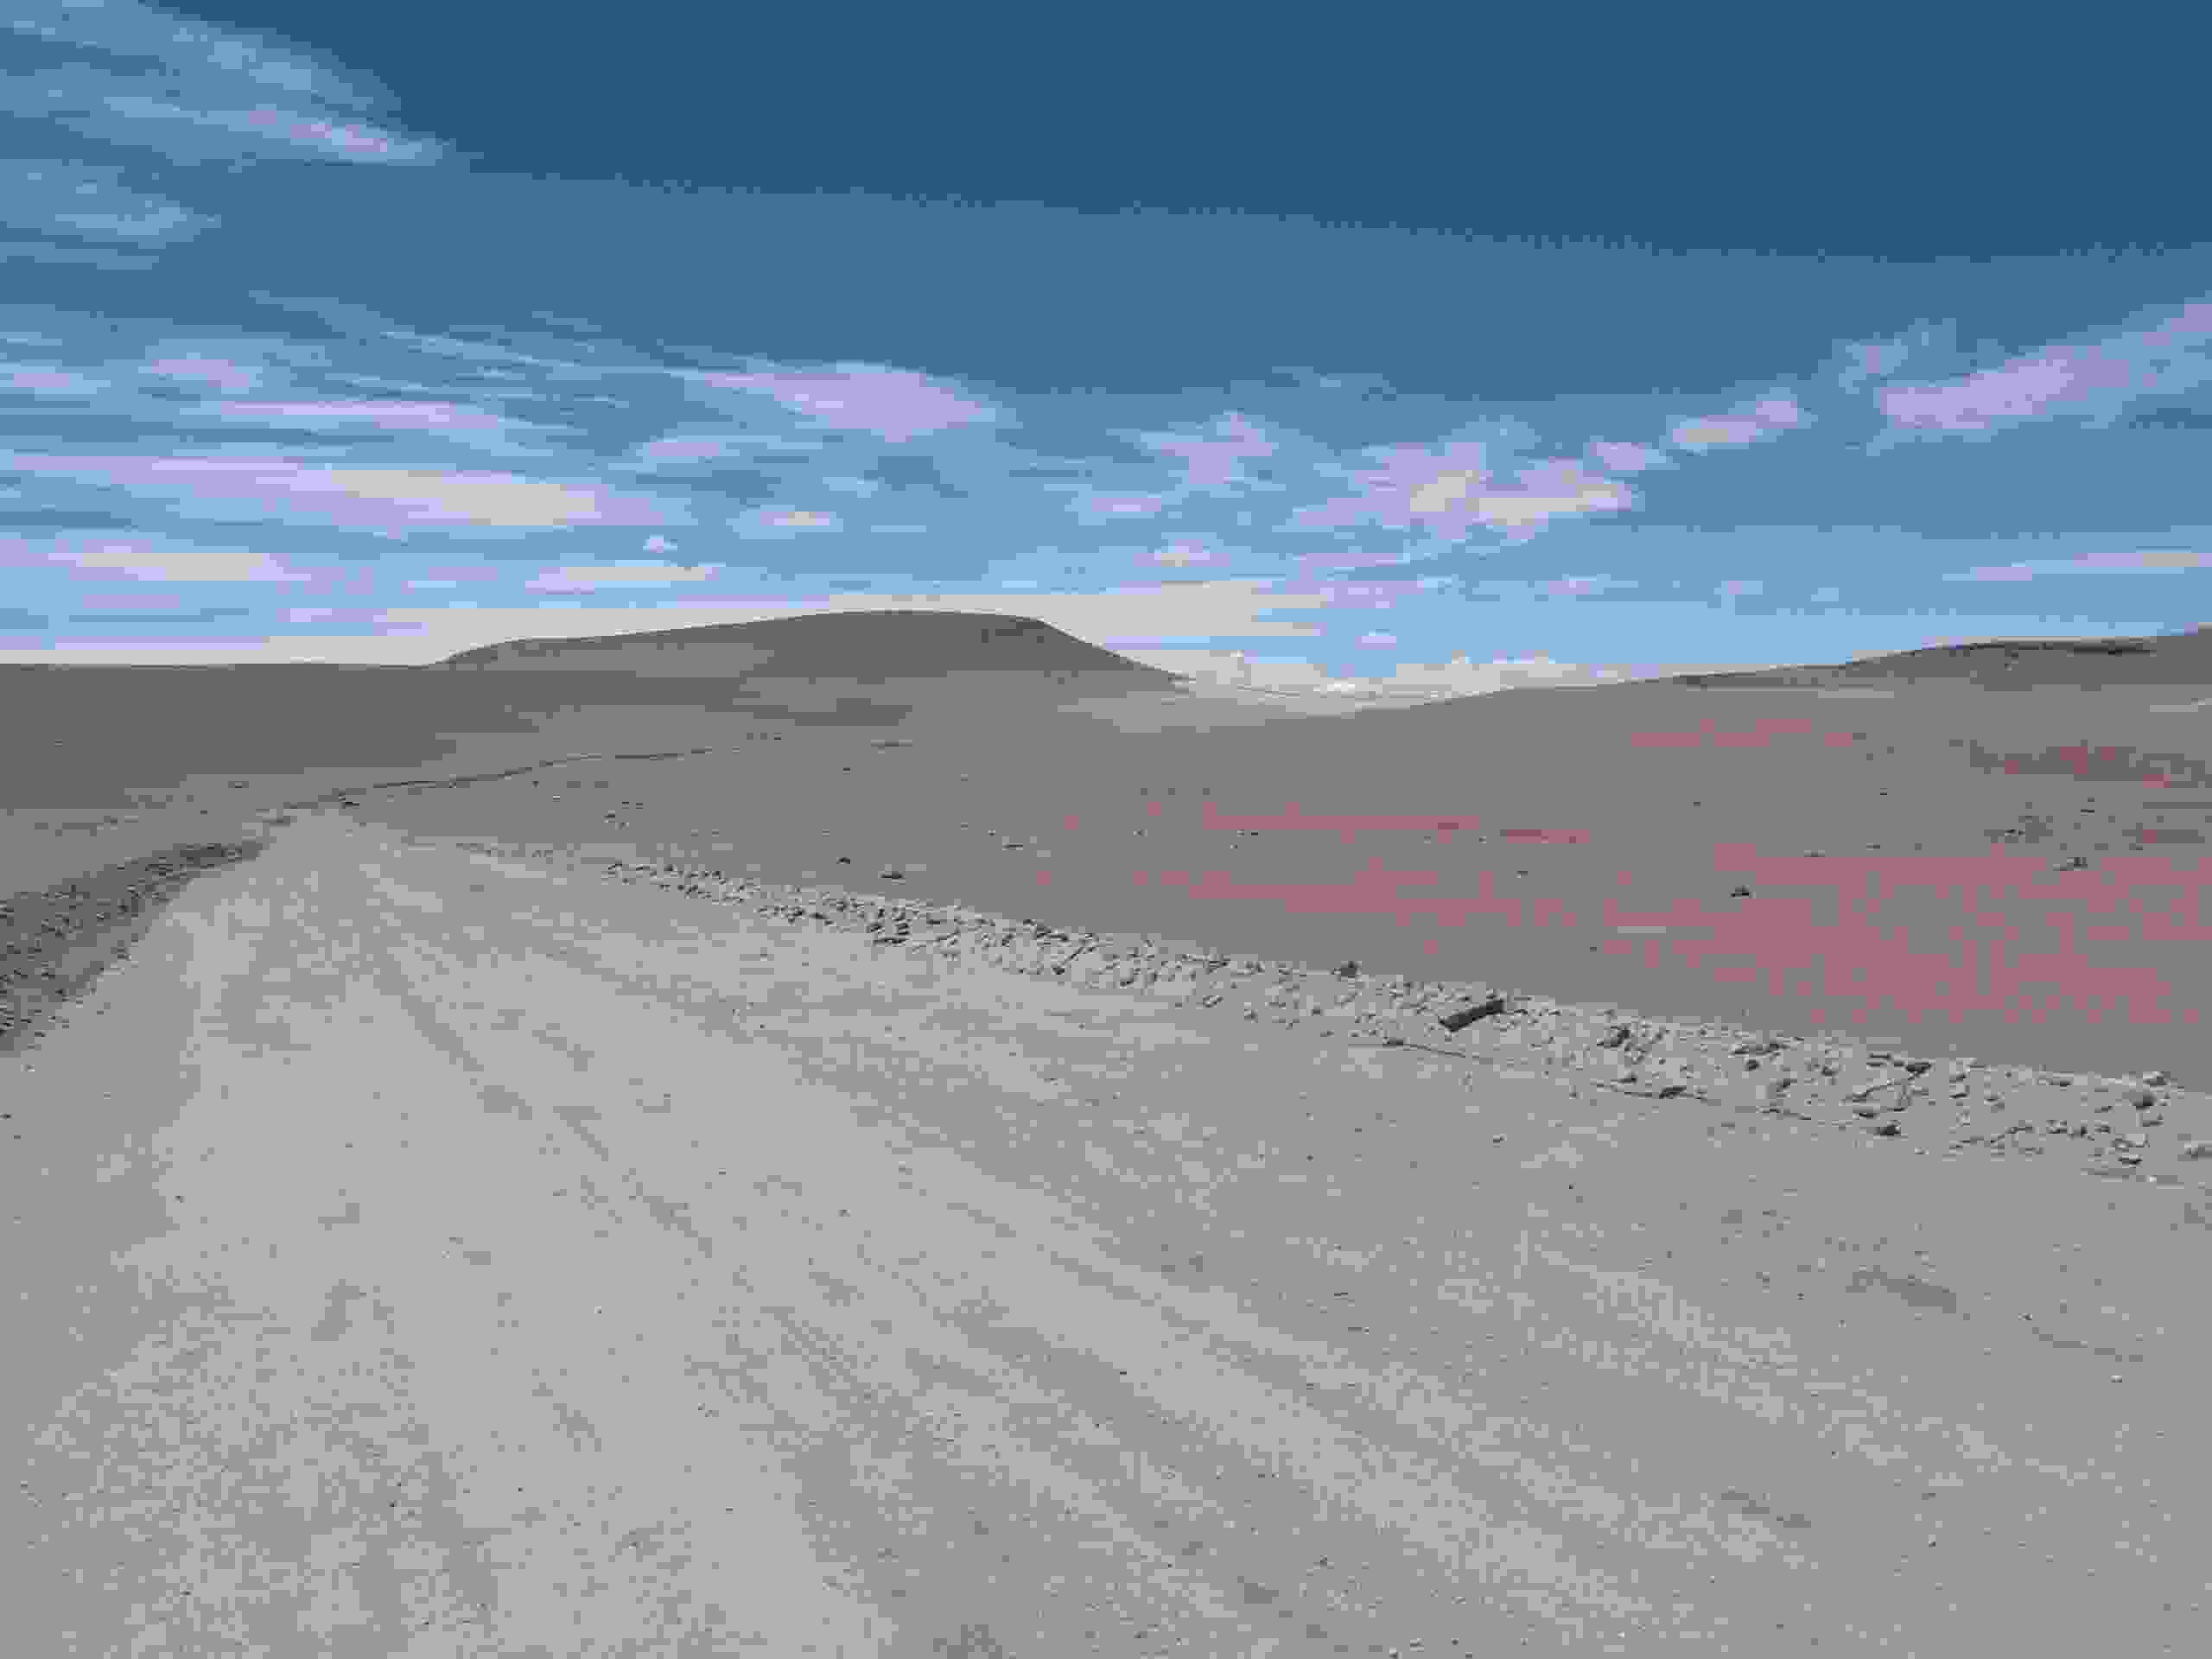
\includegraphics[width=\mywidth]{../wp-content/uploads/2015/04/wpid-wp-1427984642376.jpg} } 
 \newline
 Pour arriver au geyser de Sol de Manana à presque 5000m. \newline
 \newline
\centerline{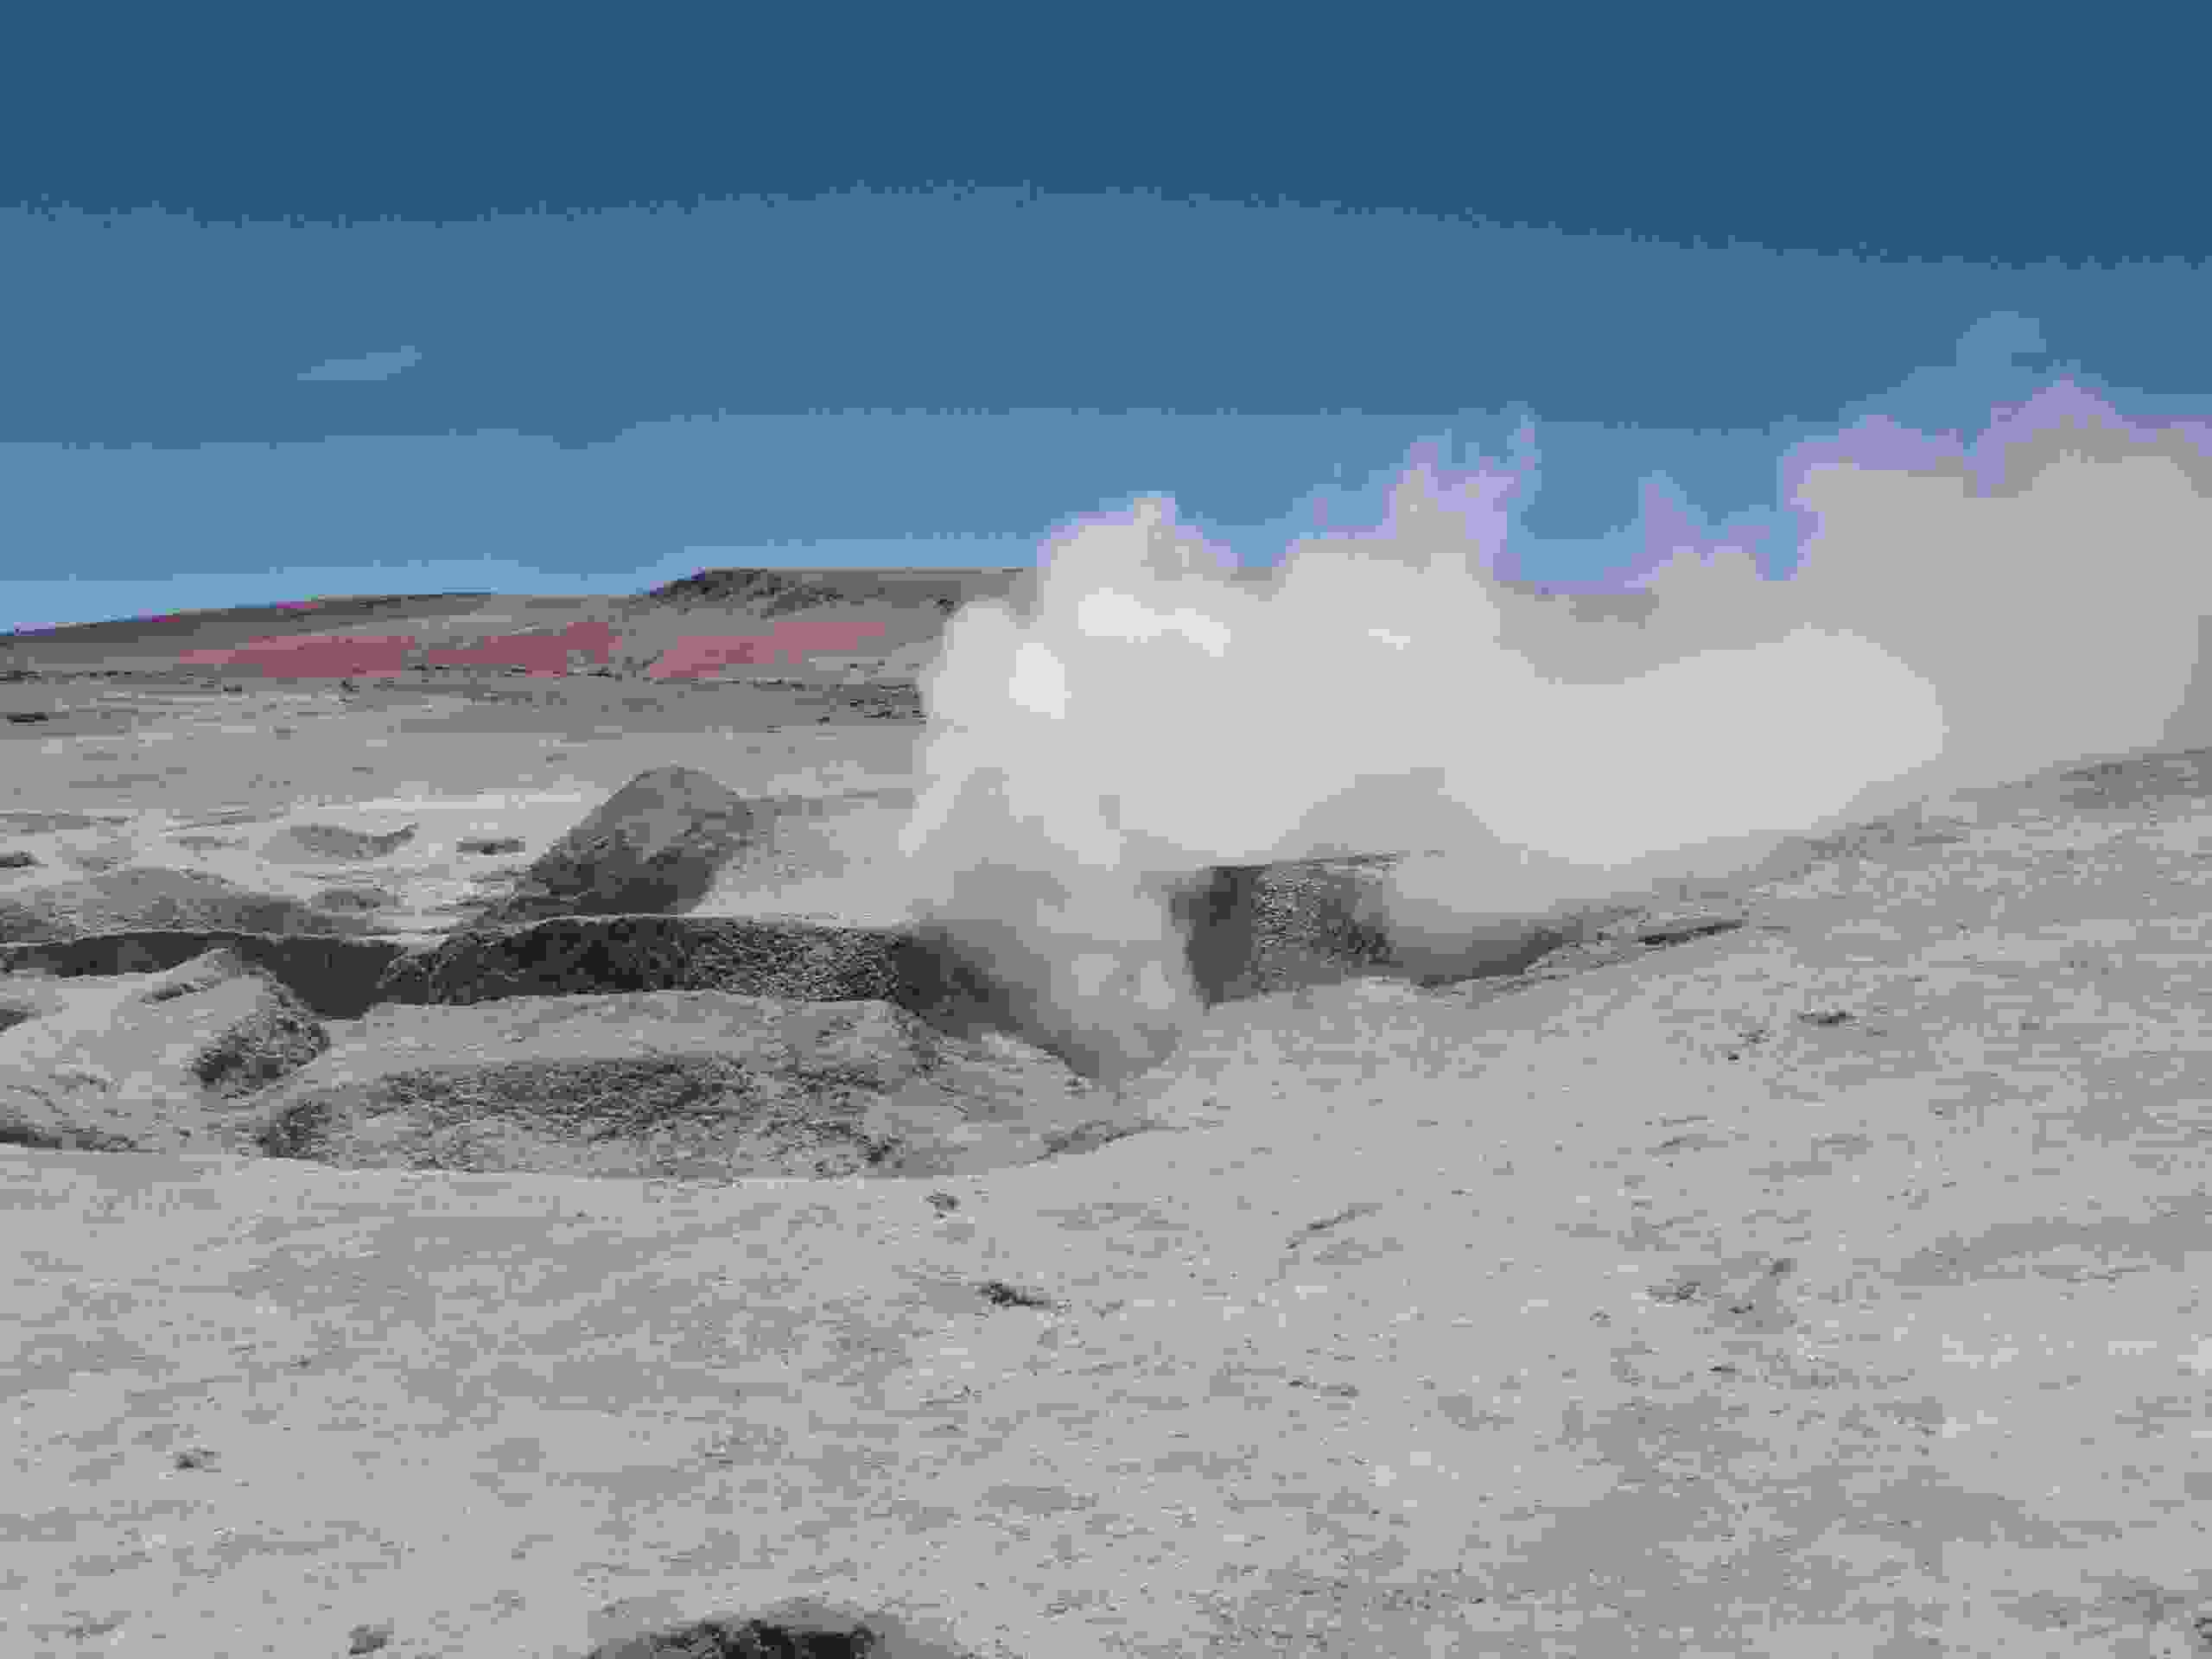
\includegraphics[width=\mywidth]{../wp-content/uploads/2015/04/wpid-wp-1427984711818.jpg} } 
 \newline
 \newline
\centerline{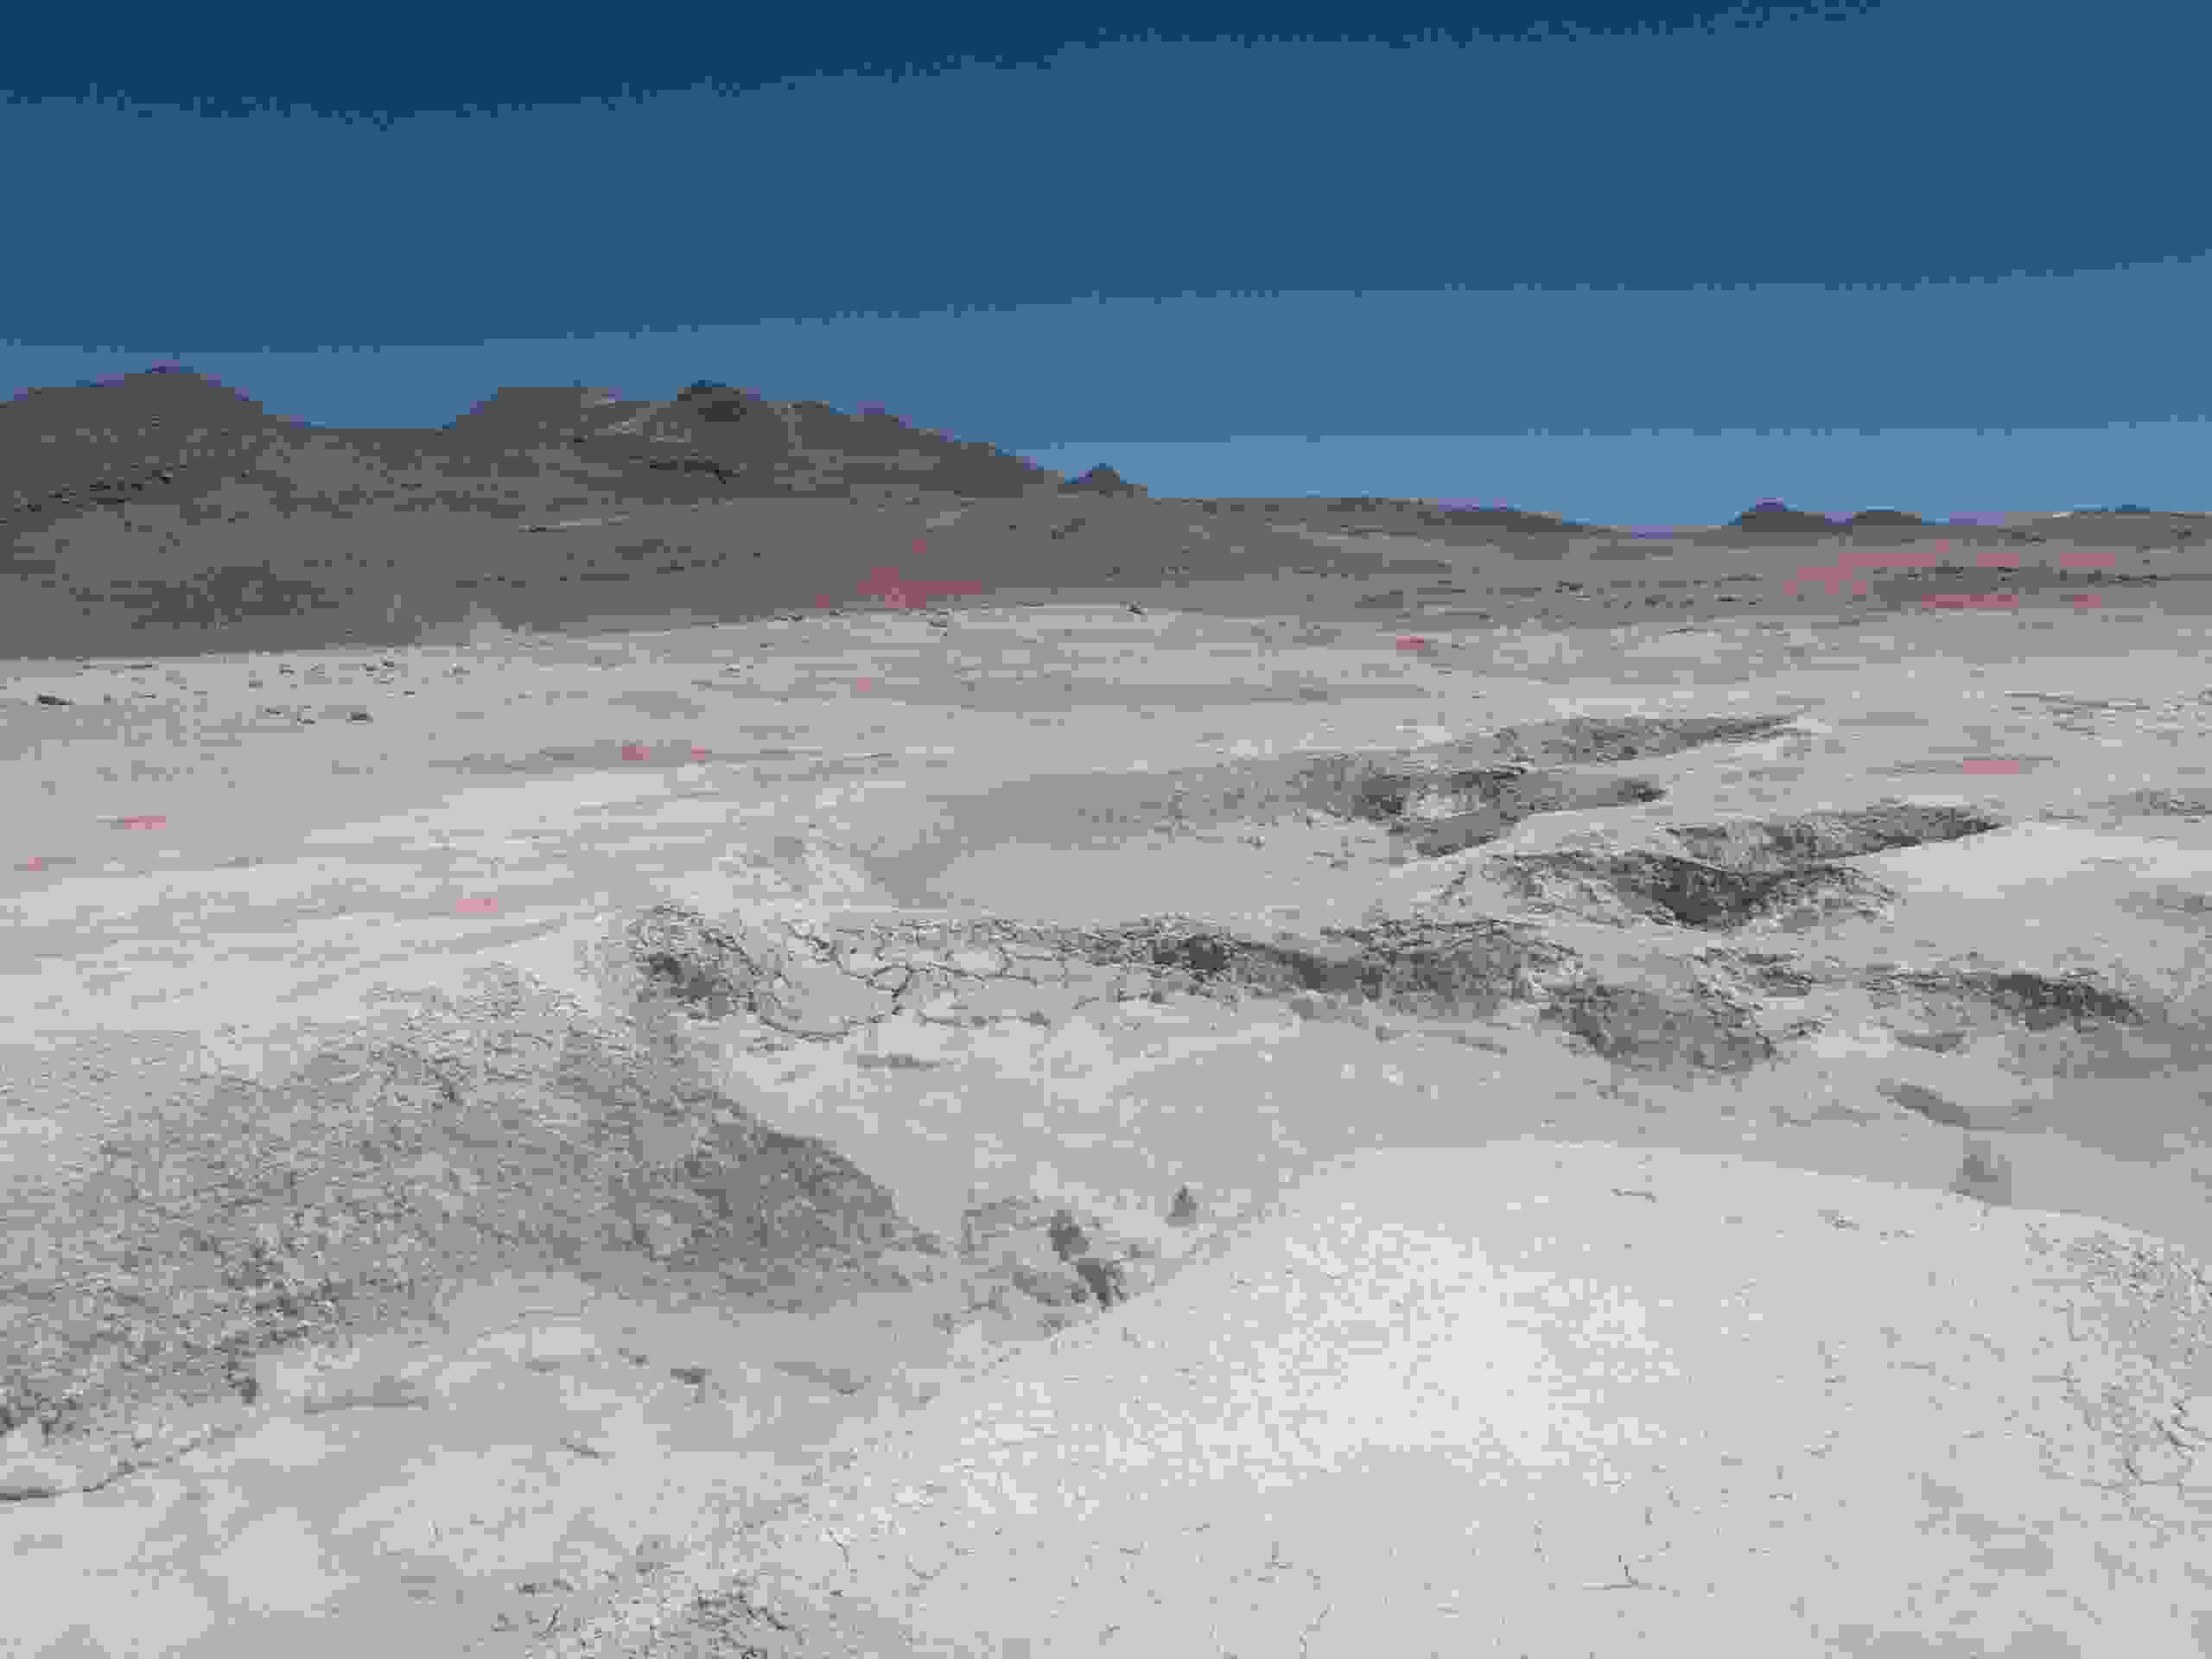
\includegraphics[width=\mywidth]{../wp-content/uploads/2015/04/wpid-wp-1427984728203.jpg} } 
 \newline
 \newline
\centerline{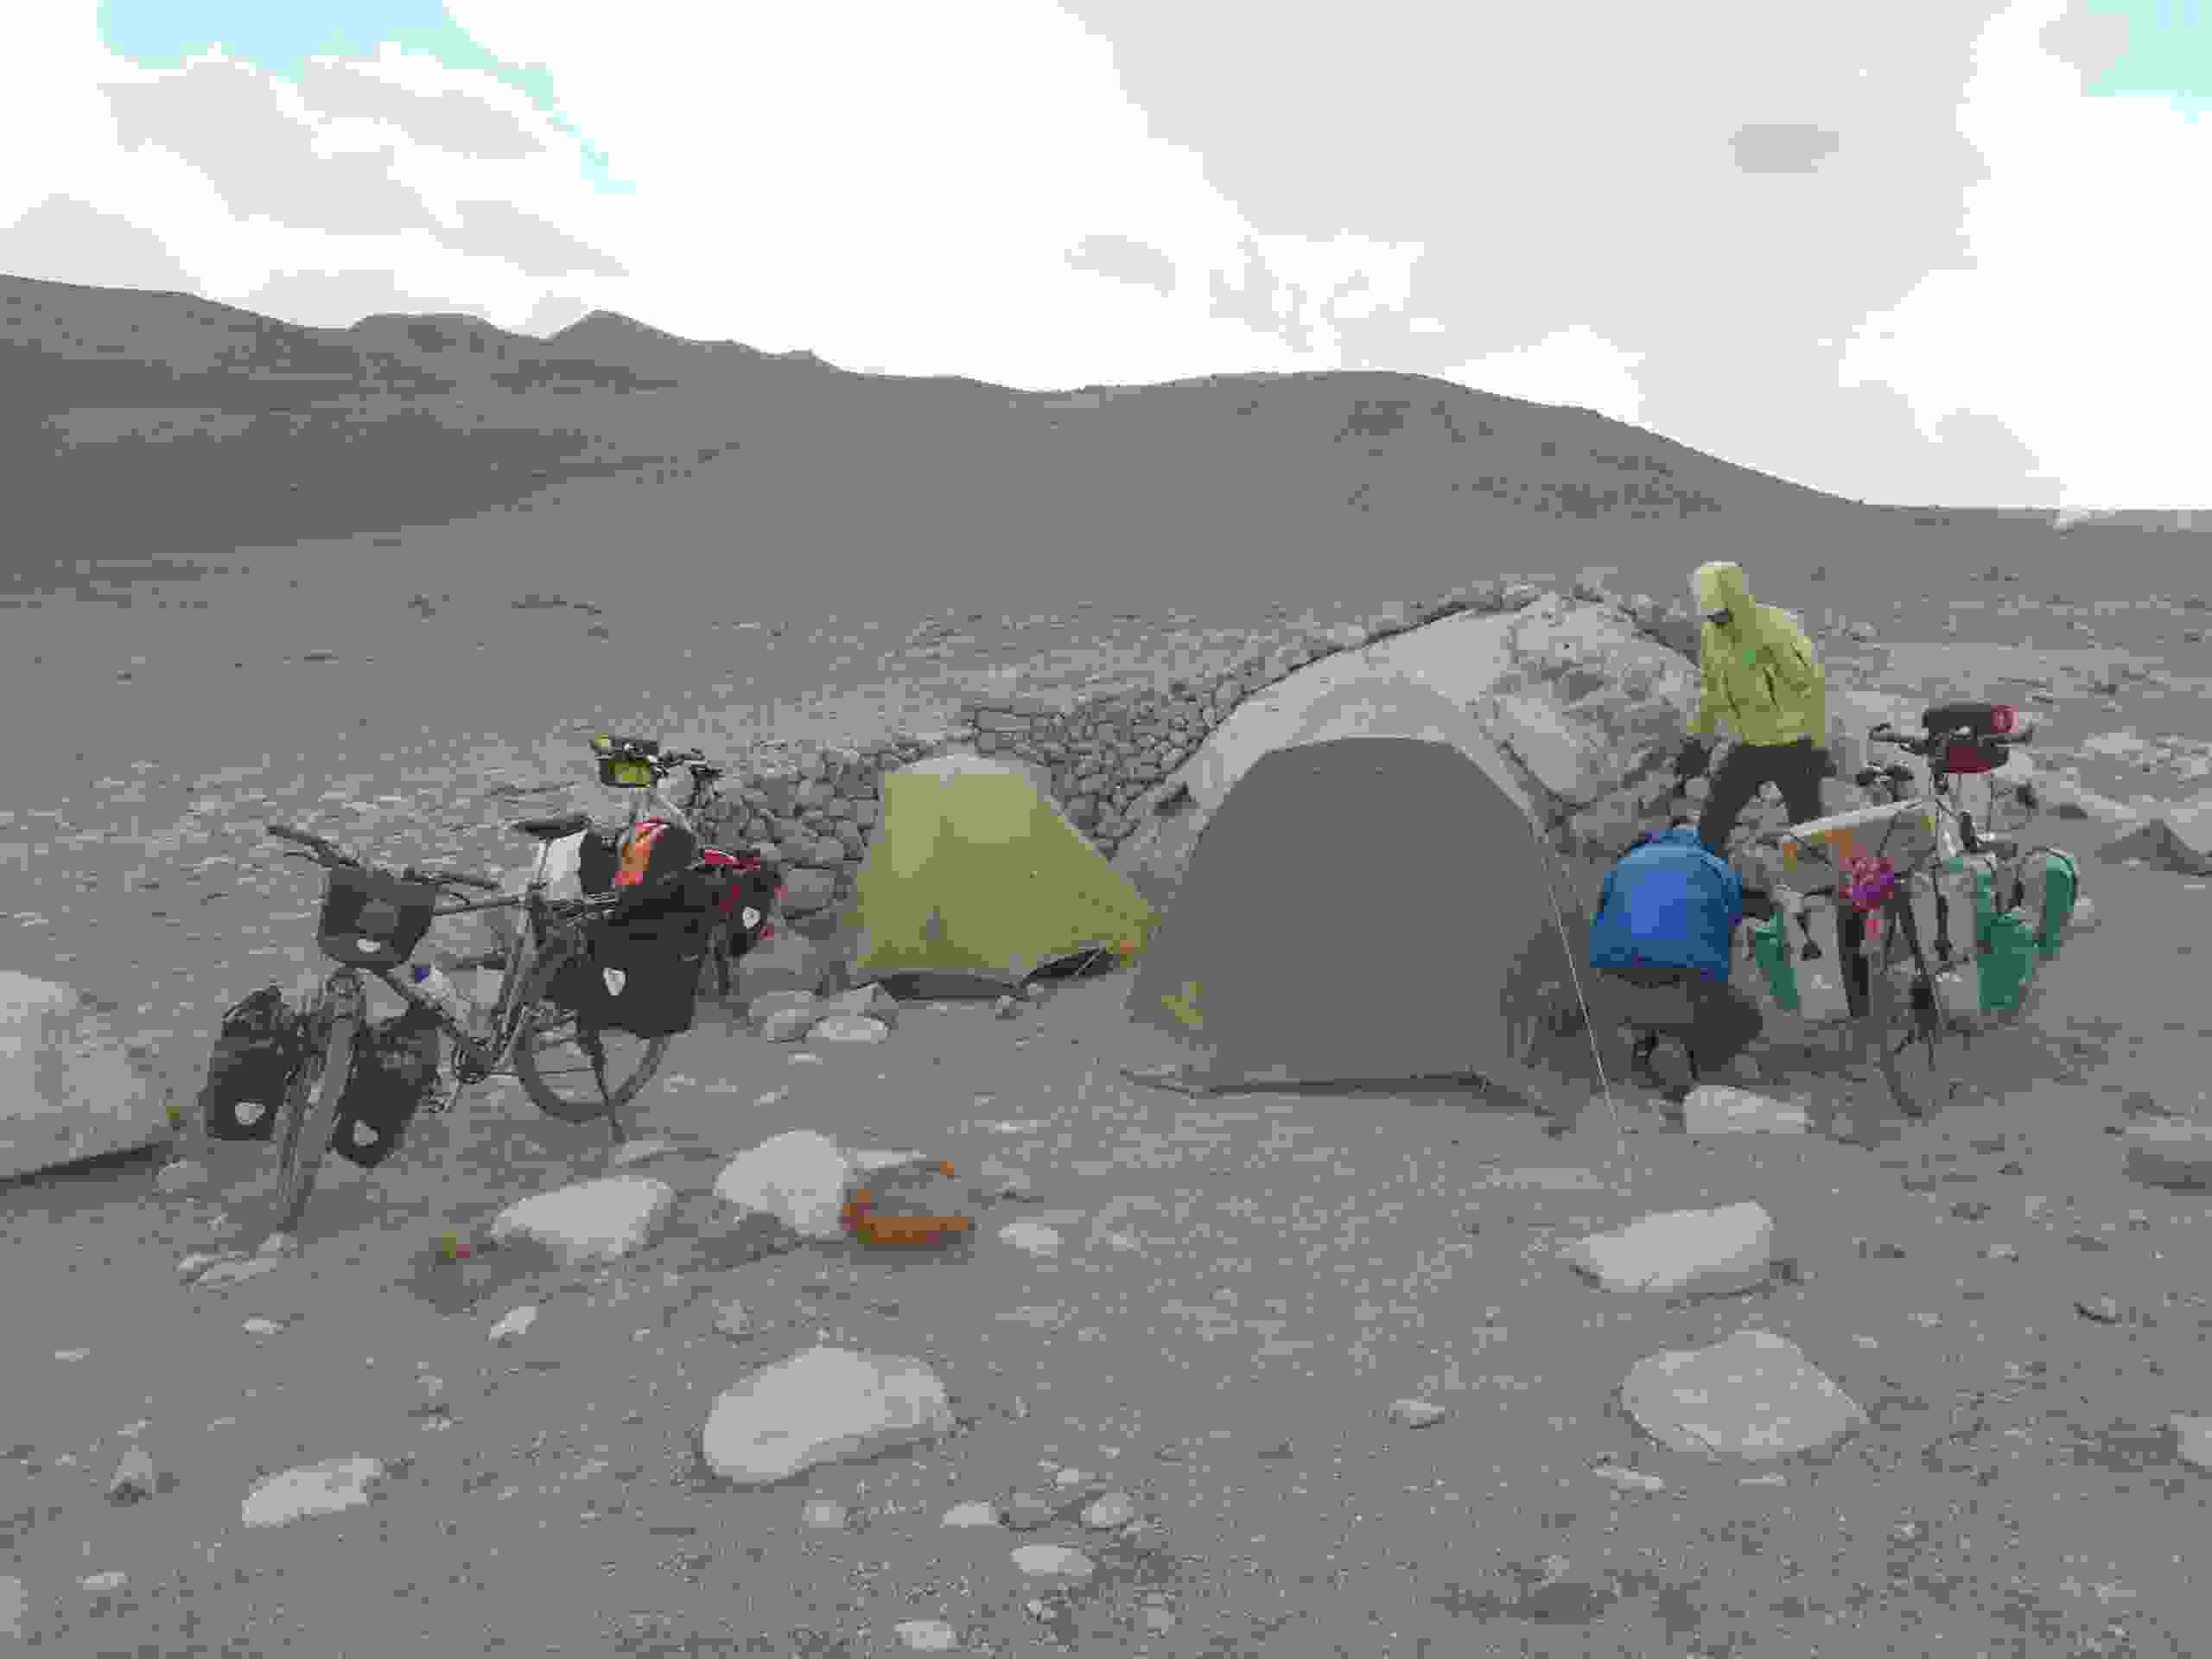
\includegraphics[width=\mywidth]{../wp-content/uploads/2015/04/wpid-wp-1427984752108.jpg} } 
 \newline
 4e jour : \newline
 Froid et vent de face, la galère commence. \newline
 \newline
\centerline{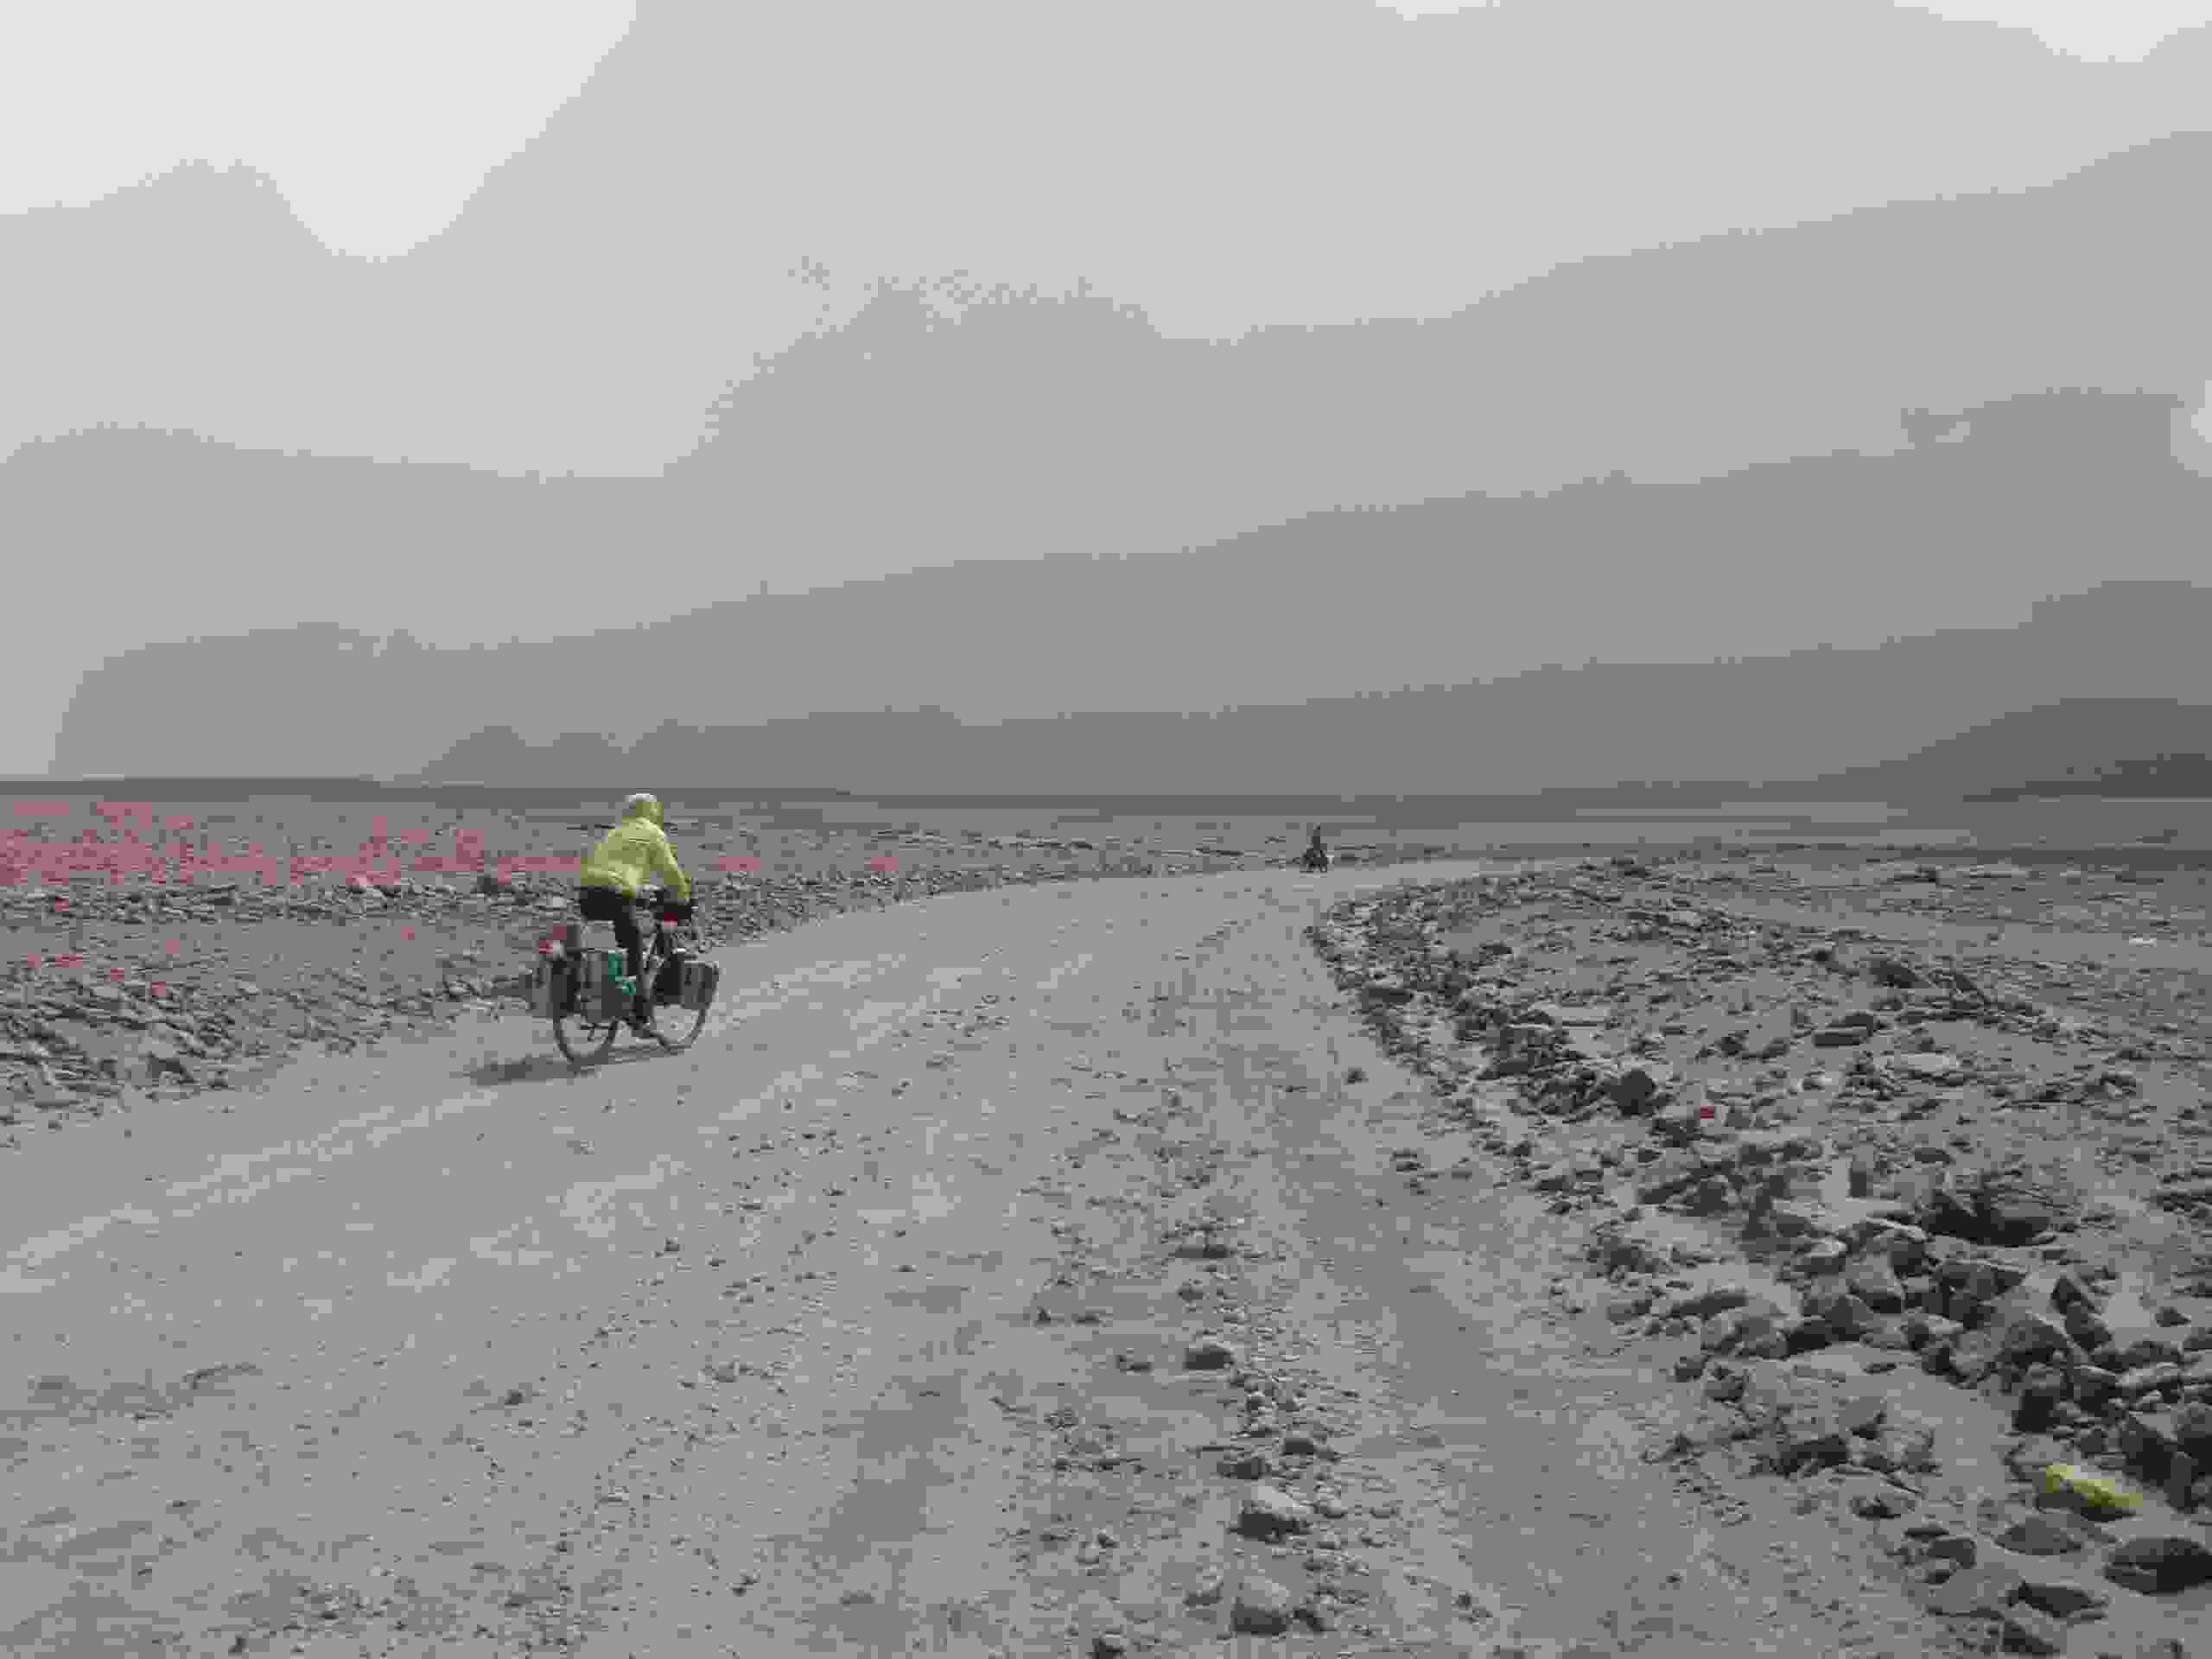
\includegraphics[width=\mywidth]{../wp-content/uploads/2015/04/wpid-wp-1427984855465.jpg} } 
 \newline
 Heureusement les premières vues sur la Laguna Colorado compensent un peu. \newline
 \newline
\centerline{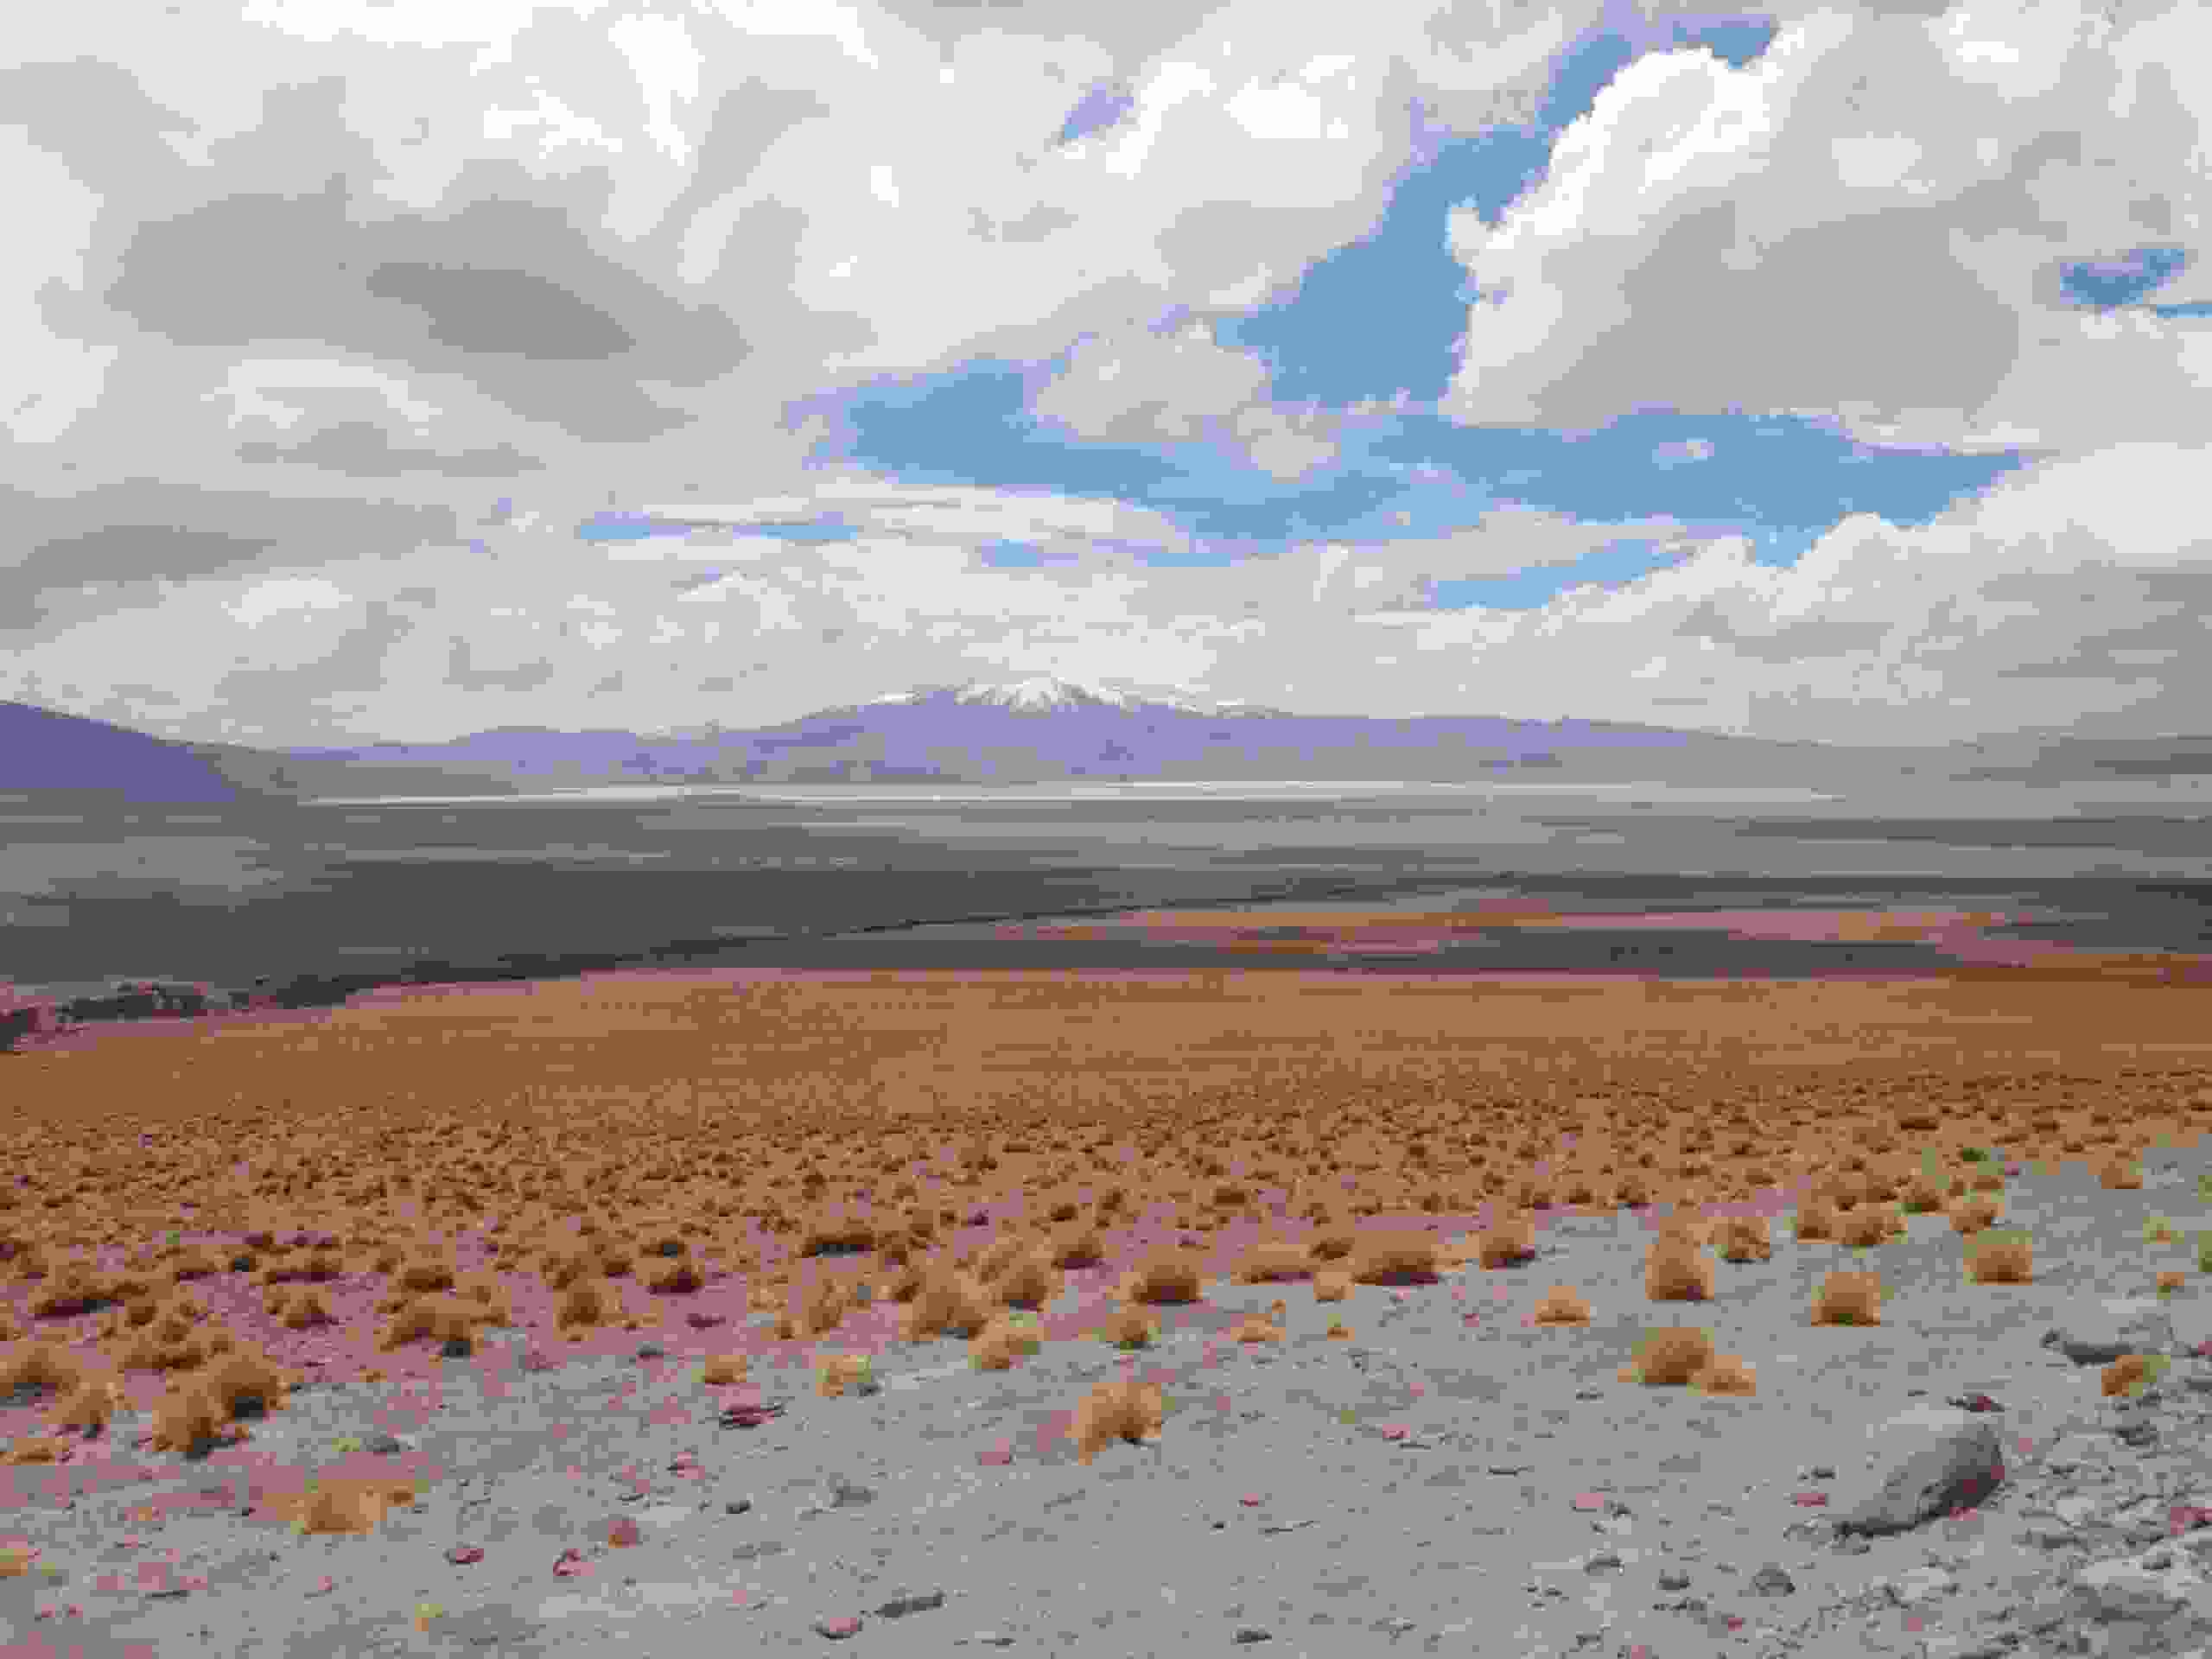
\includegraphics[width=\mywidth]{../wp-content/uploads/2015/04/wpid-wp-1427984806510.jpg} } 
 \newline
 \newline
\centerline{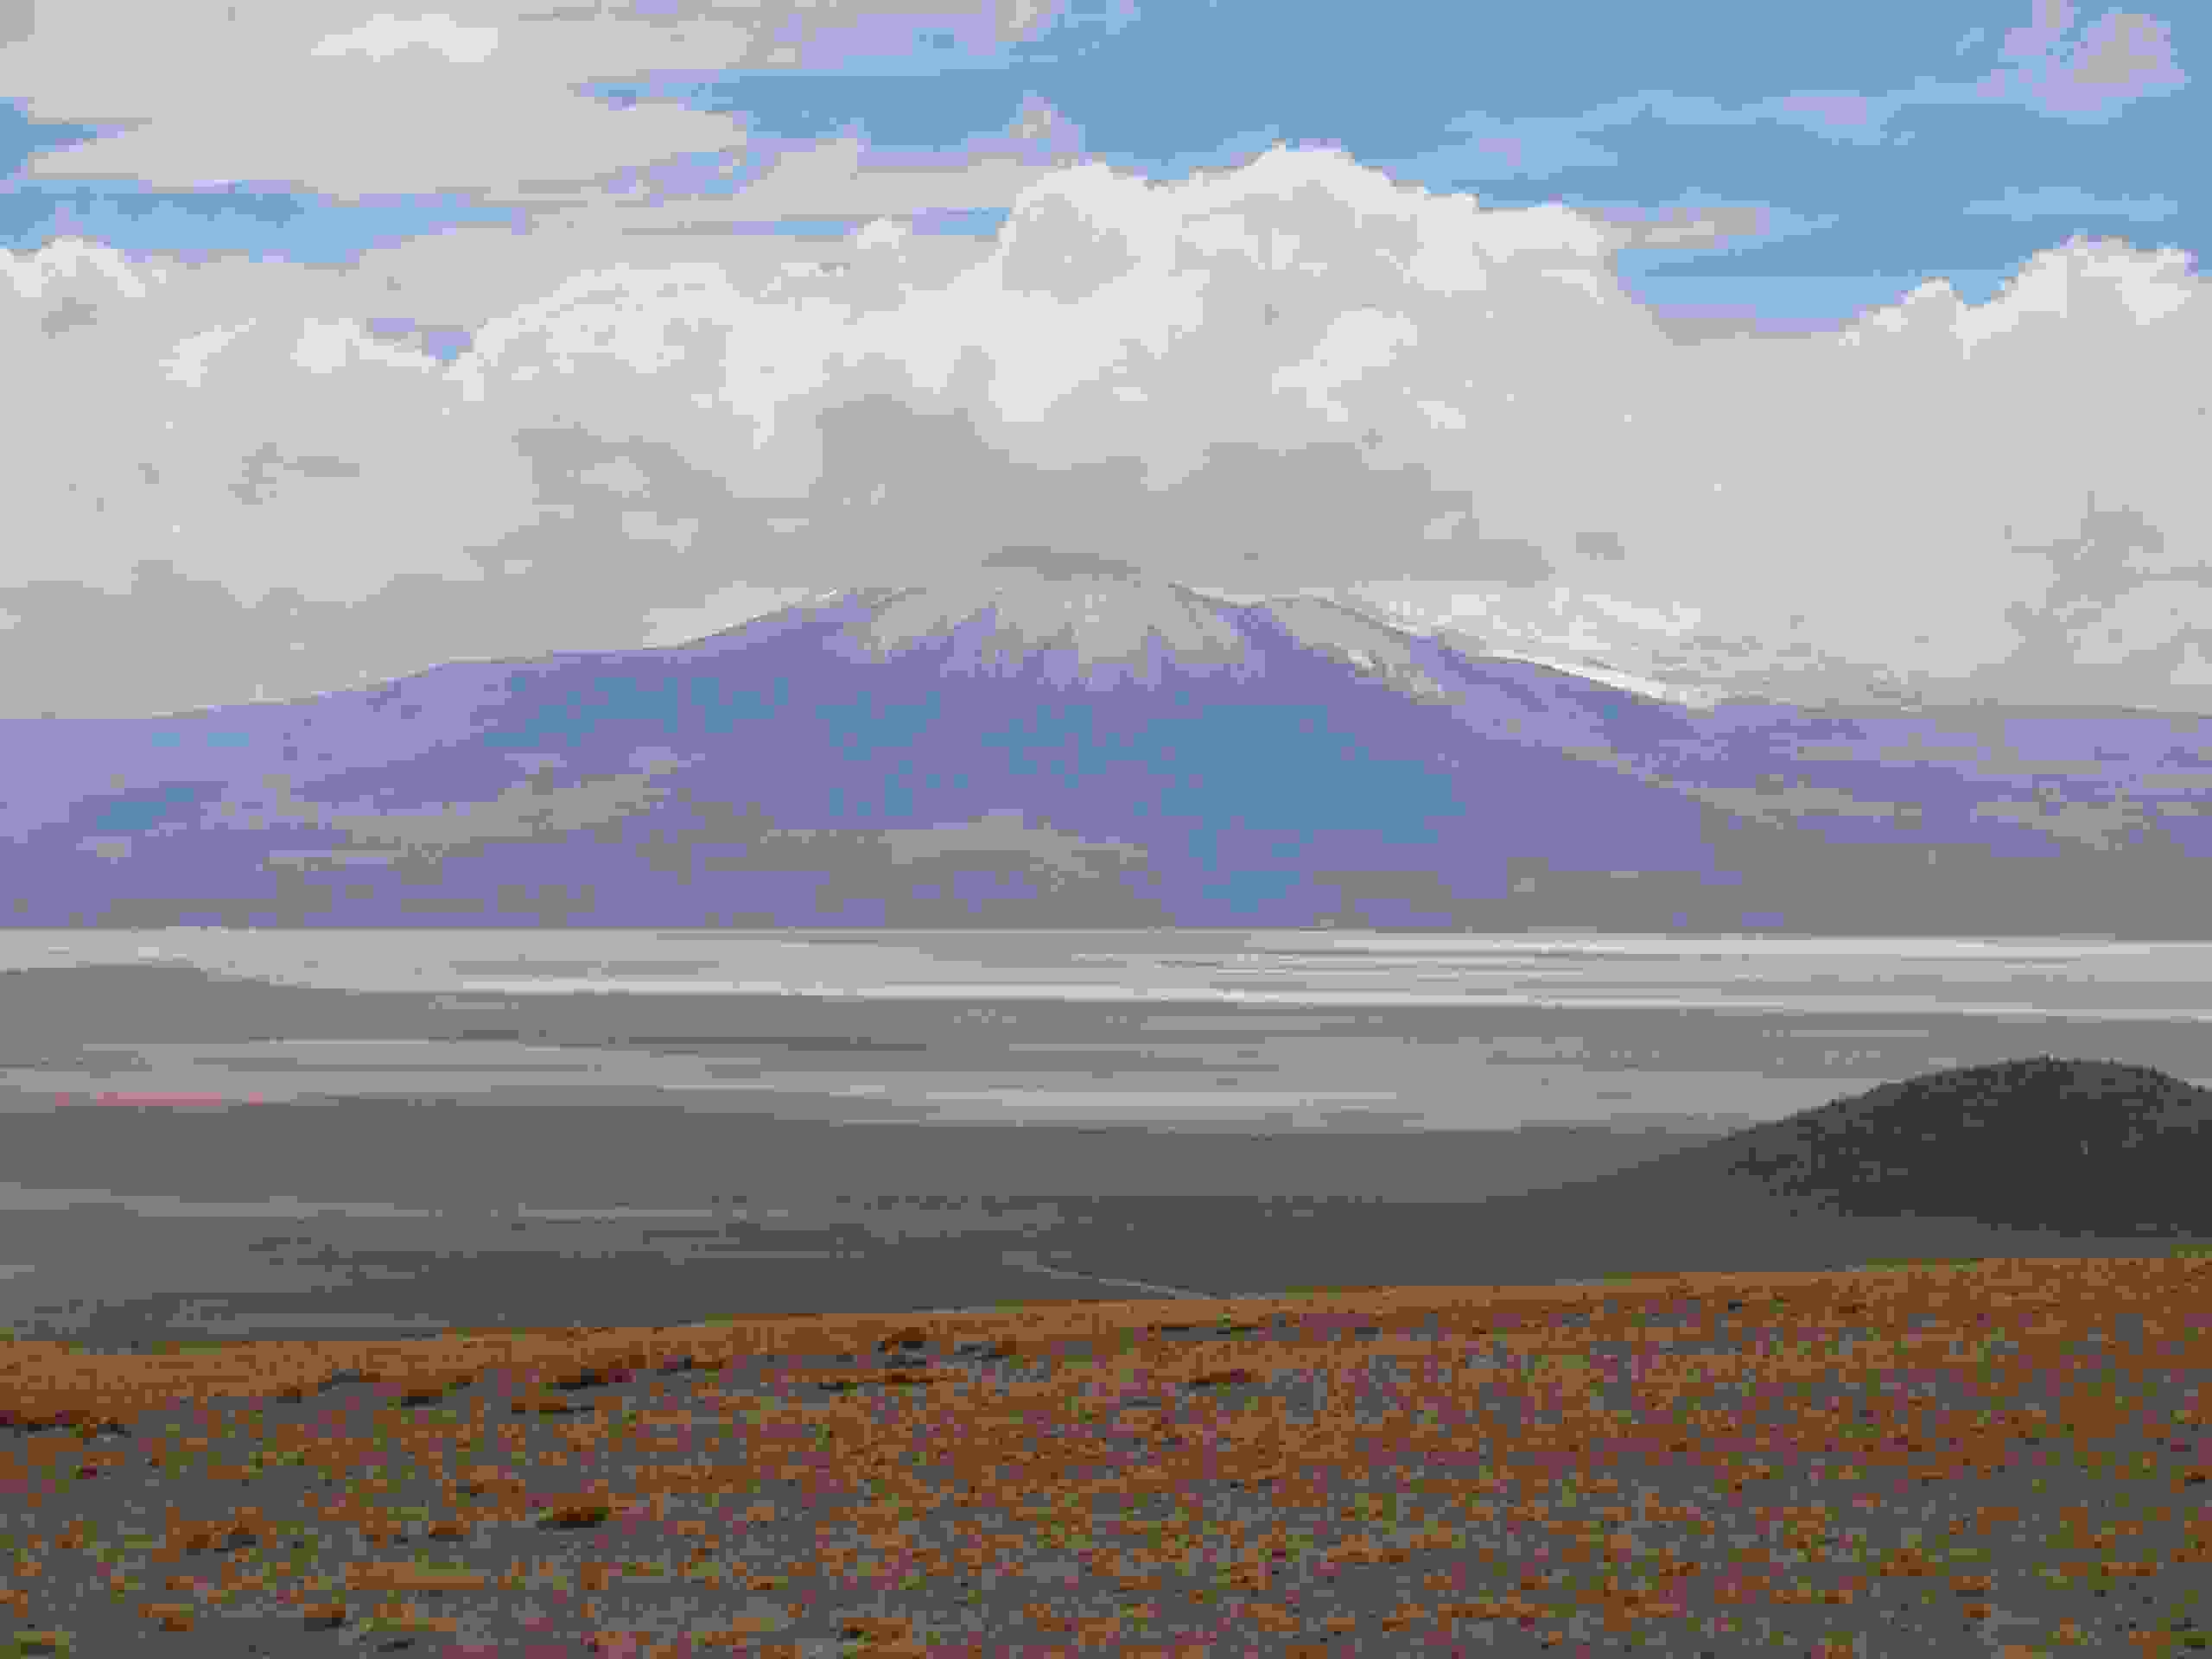
\includegraphics[width=\mywidth]{../wp-content/uploads/2015/04/wpid-wp-1427984819618.jpg} } 
 \newline
 En plus du vent la pluie arrive, on s'arrête plus tôt que prévu dans un refuge et on reste dormir dans un dortoir. \newline
 \newline
\centerline{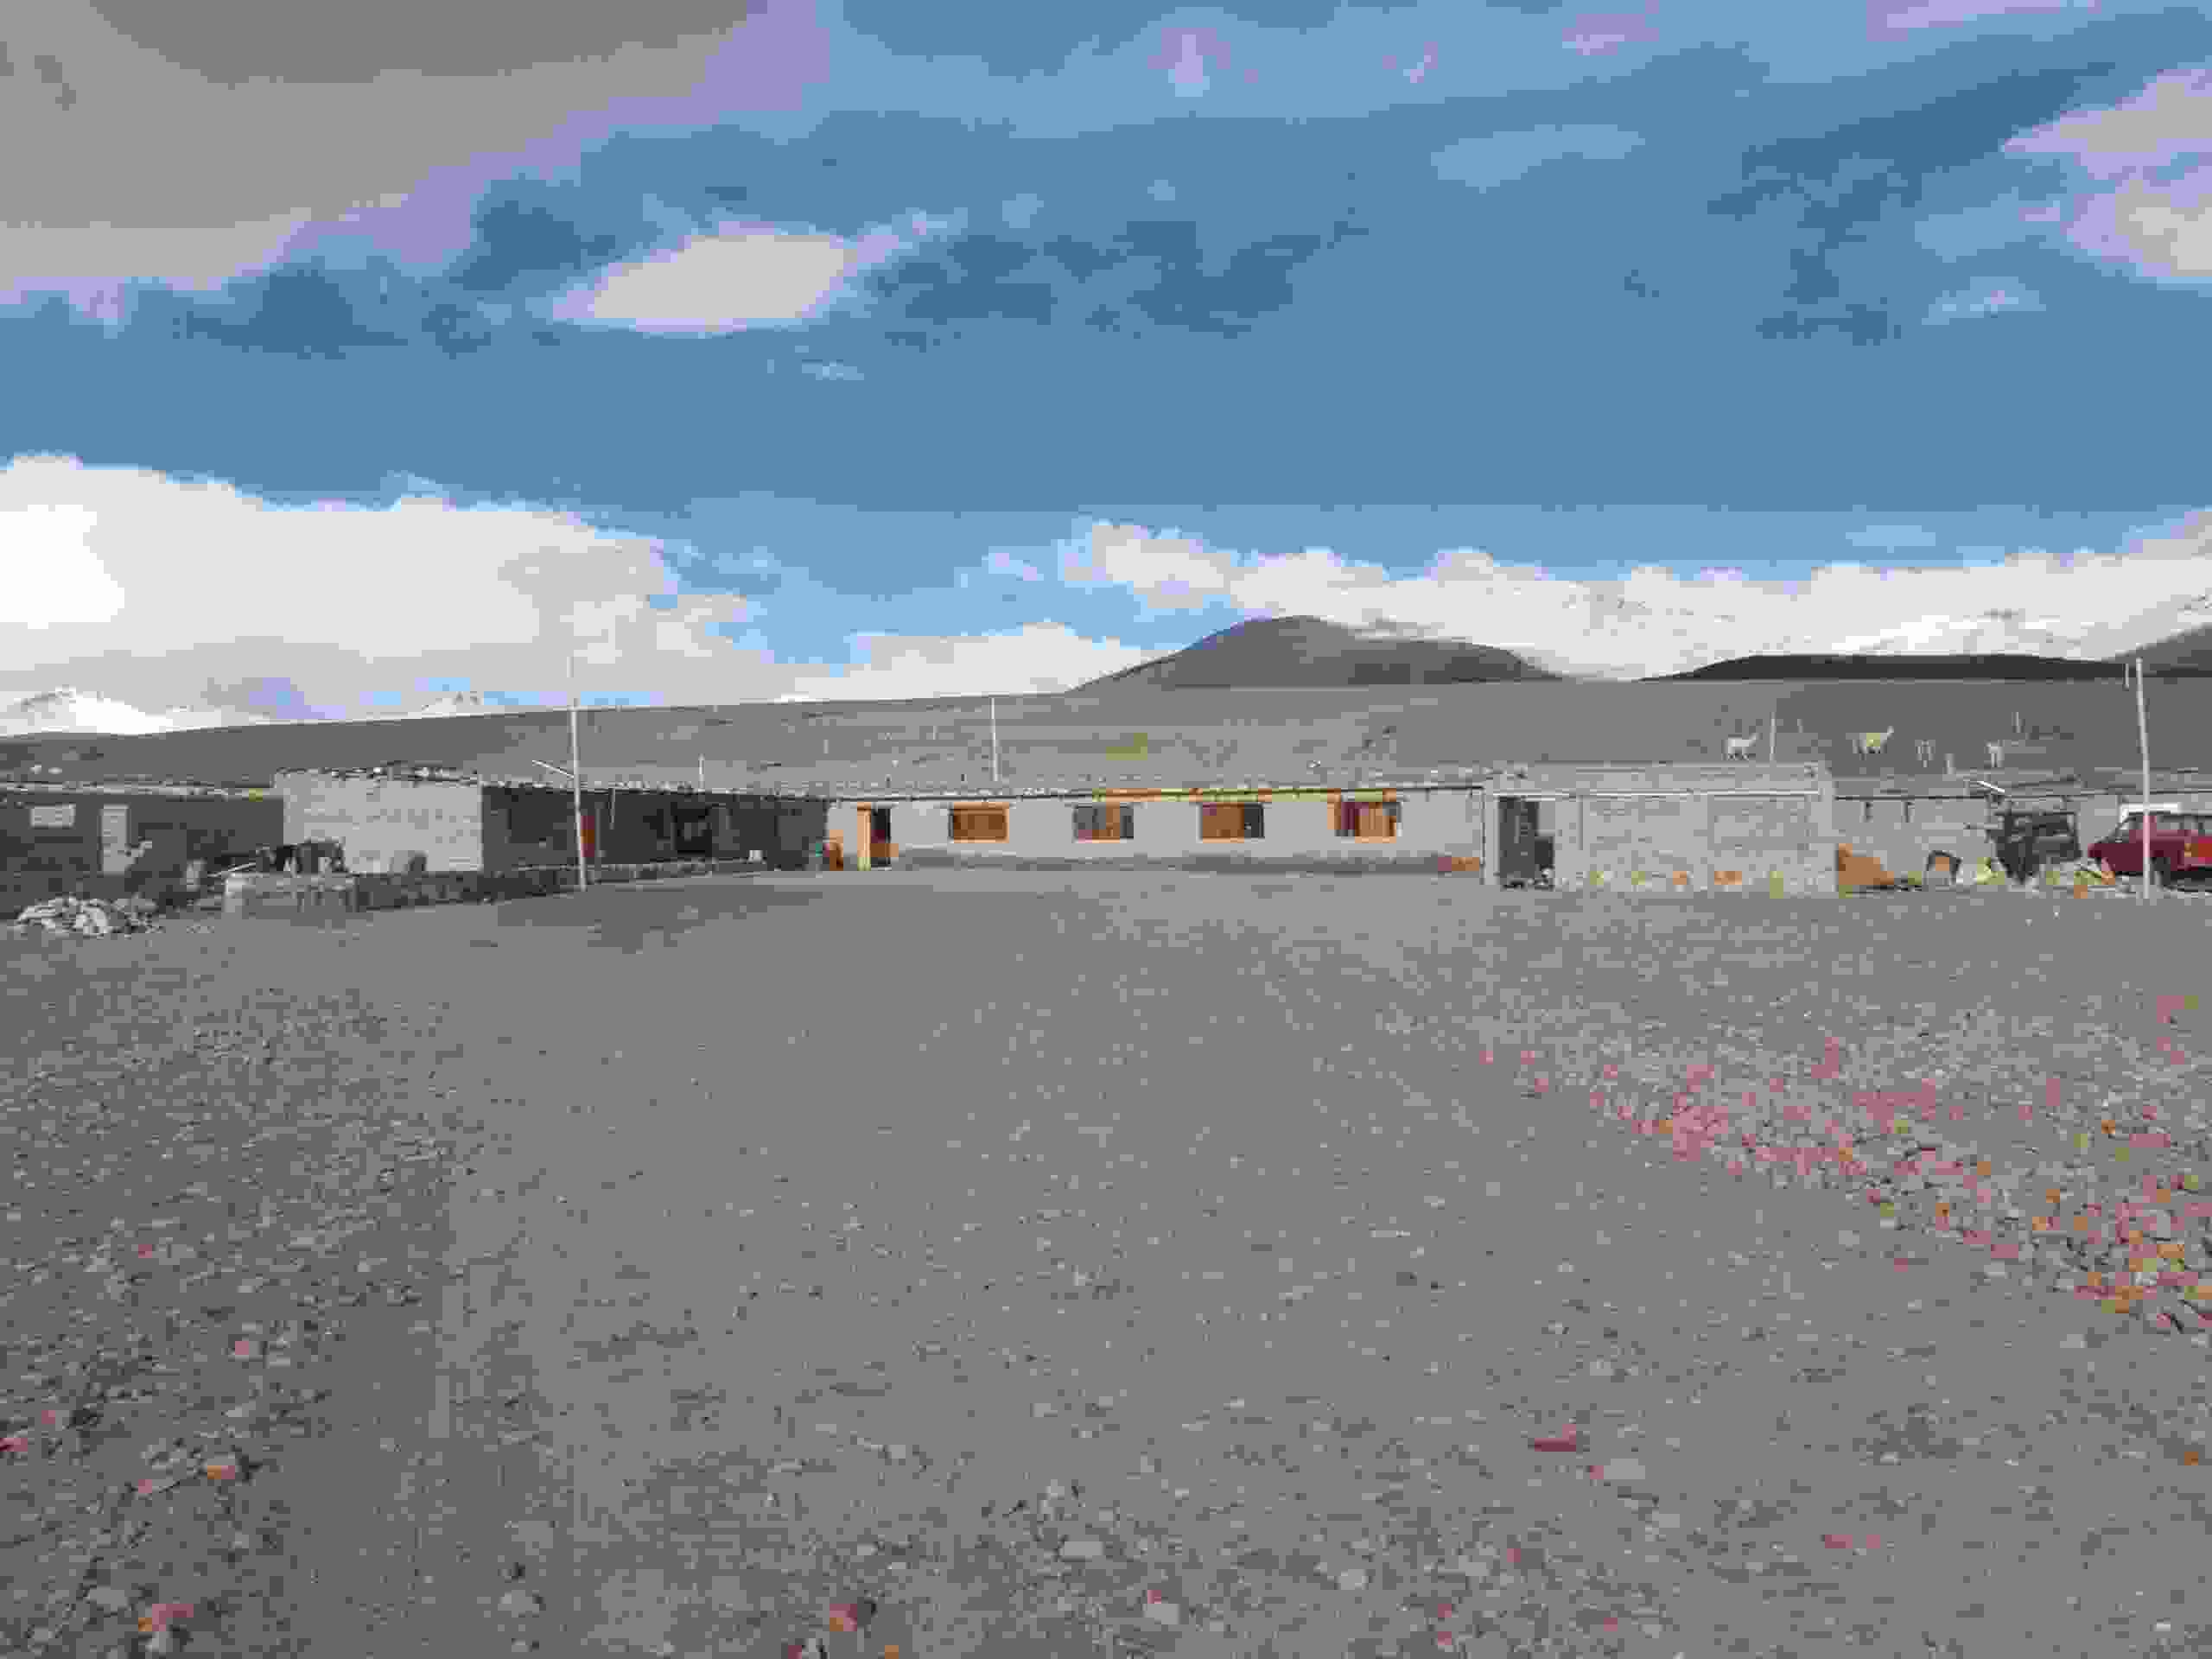
\includegraphics[width=\mywidth]{../wp-content/uploads/2015/04/wpid-wp-1427984897297.jpg} } 
 \newline
 5e jour : \newline
 10km dans le sable pour arriver au ravitaillement : on s'est fait déposer un carton de nourriture dans un refuge. \newline
 \newline
\centerline{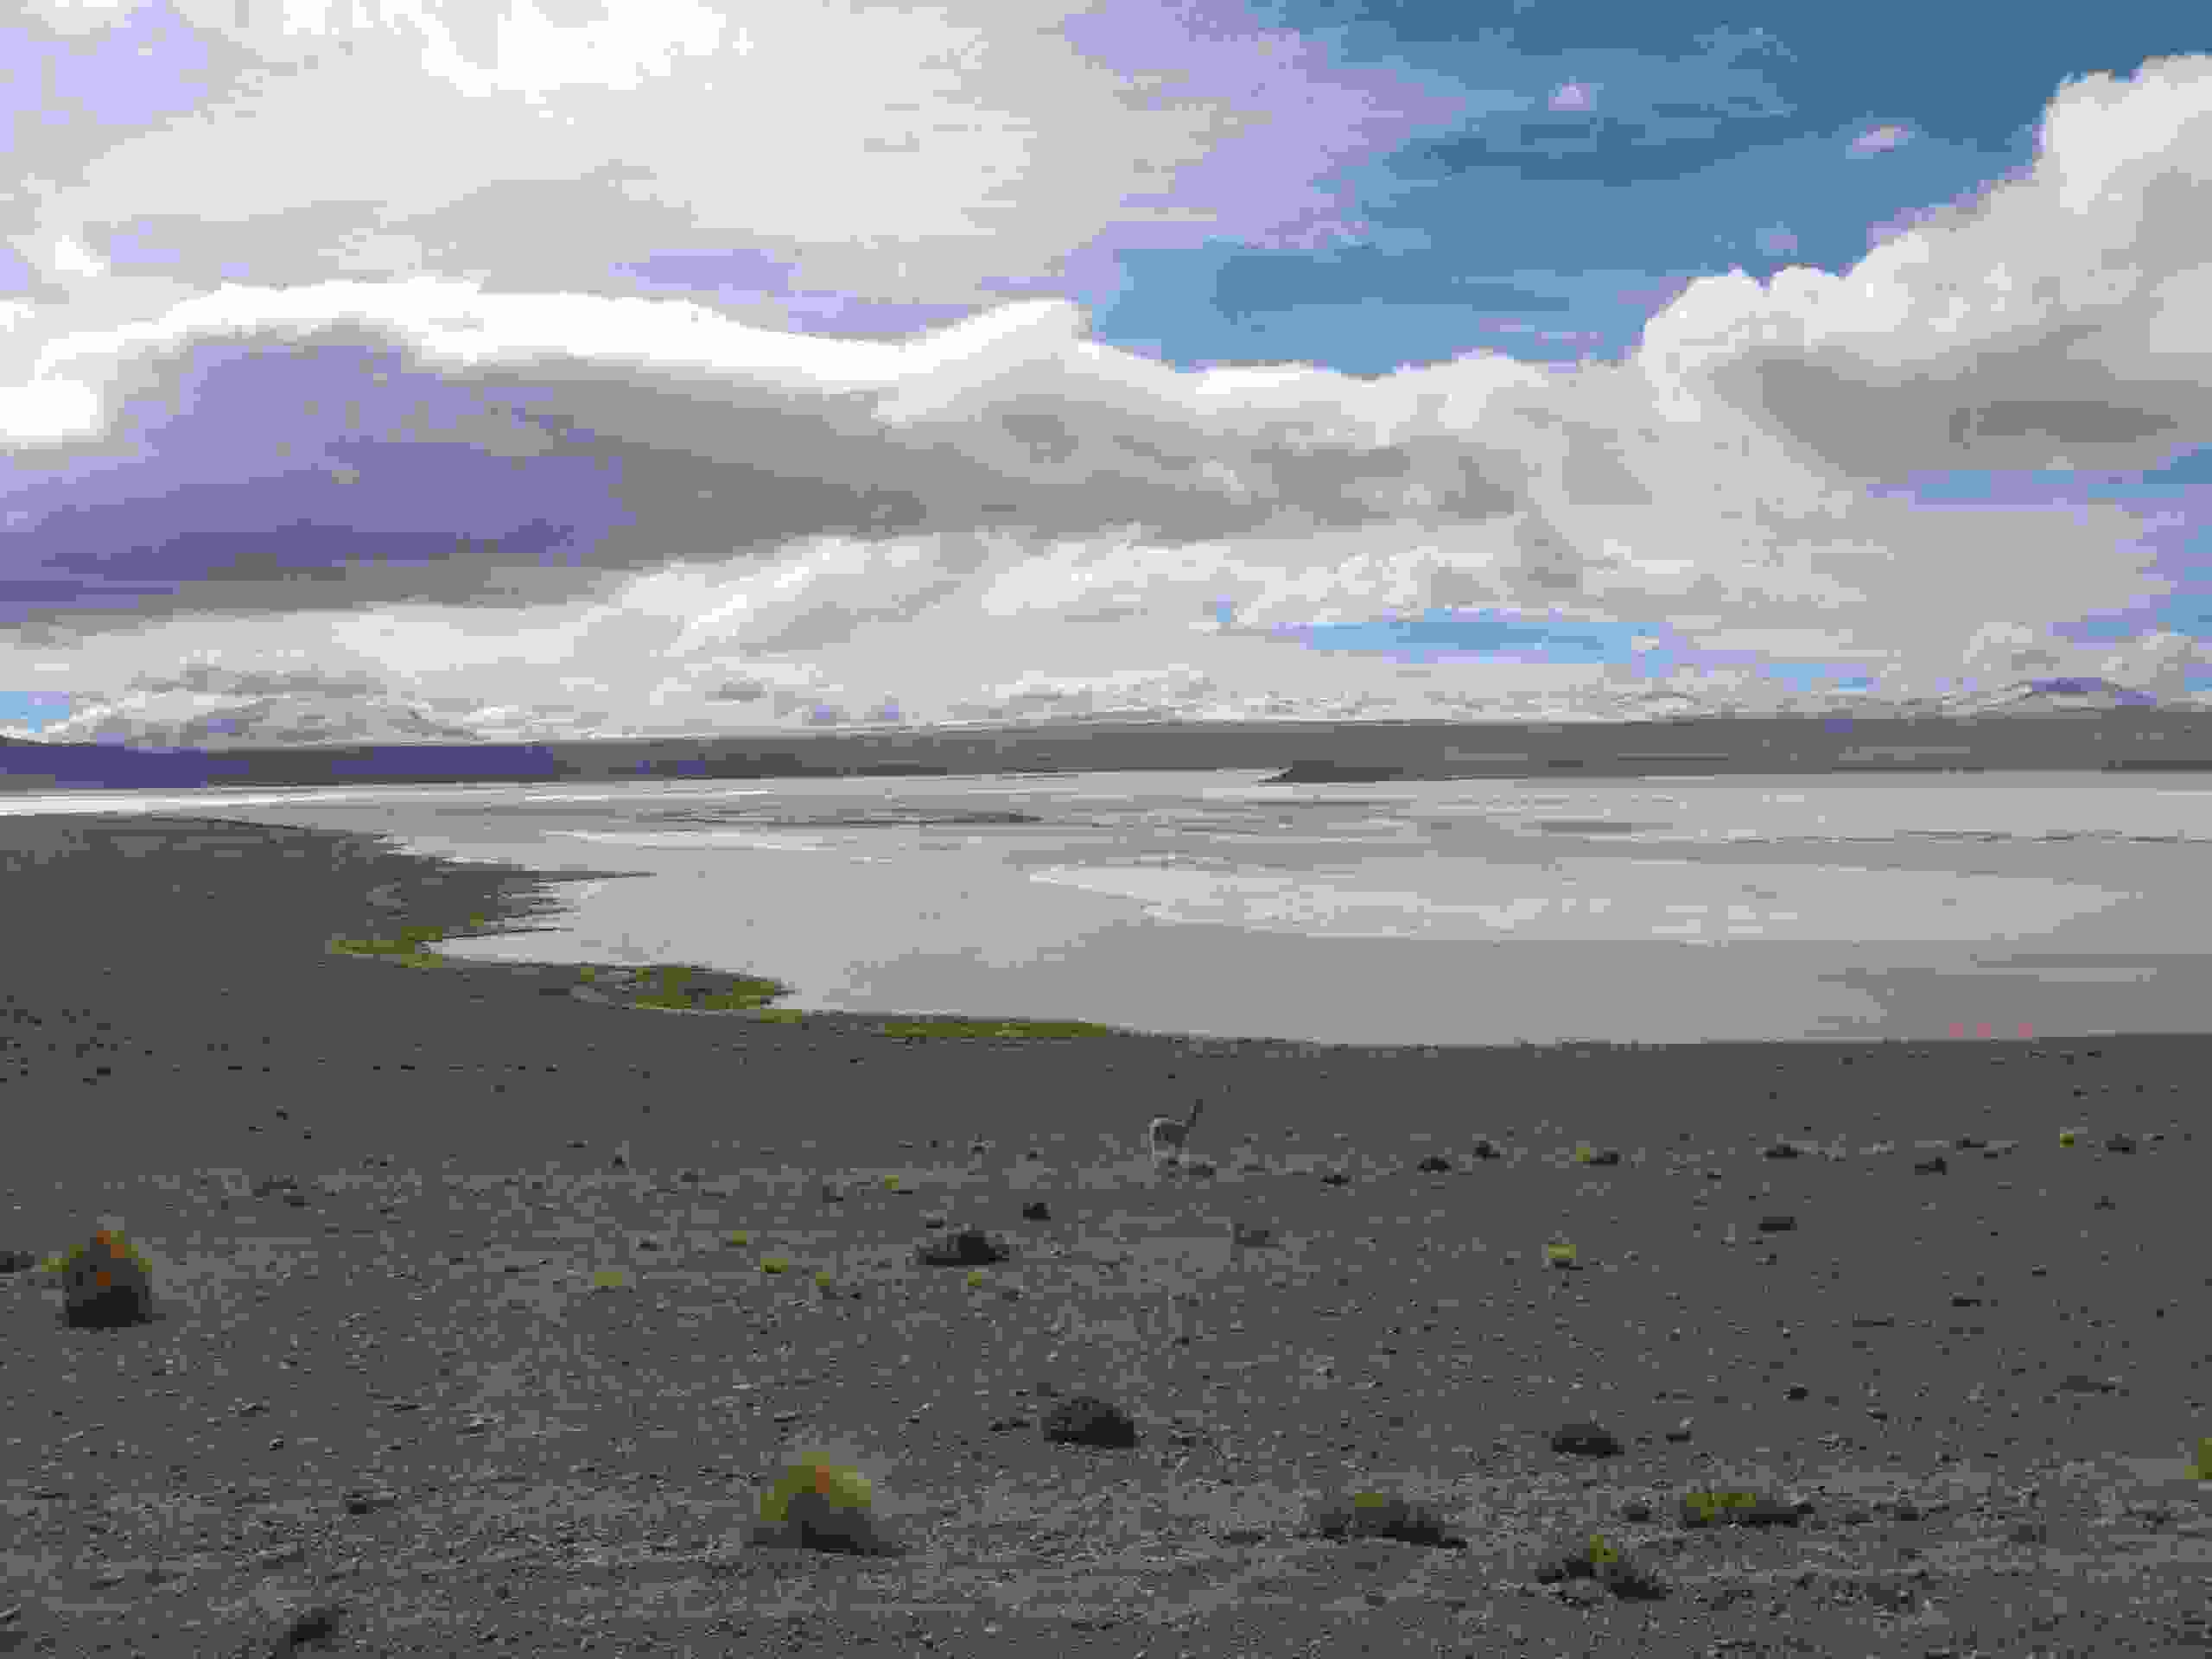
\includegraphics[width=\mywidth]{../wp-content/uploads/2015/04/wpid-wp-1427984947015.jpg} } 
 \newline
 Ça continue à monter avec le vent de face. \newline
 \newline
\centerline{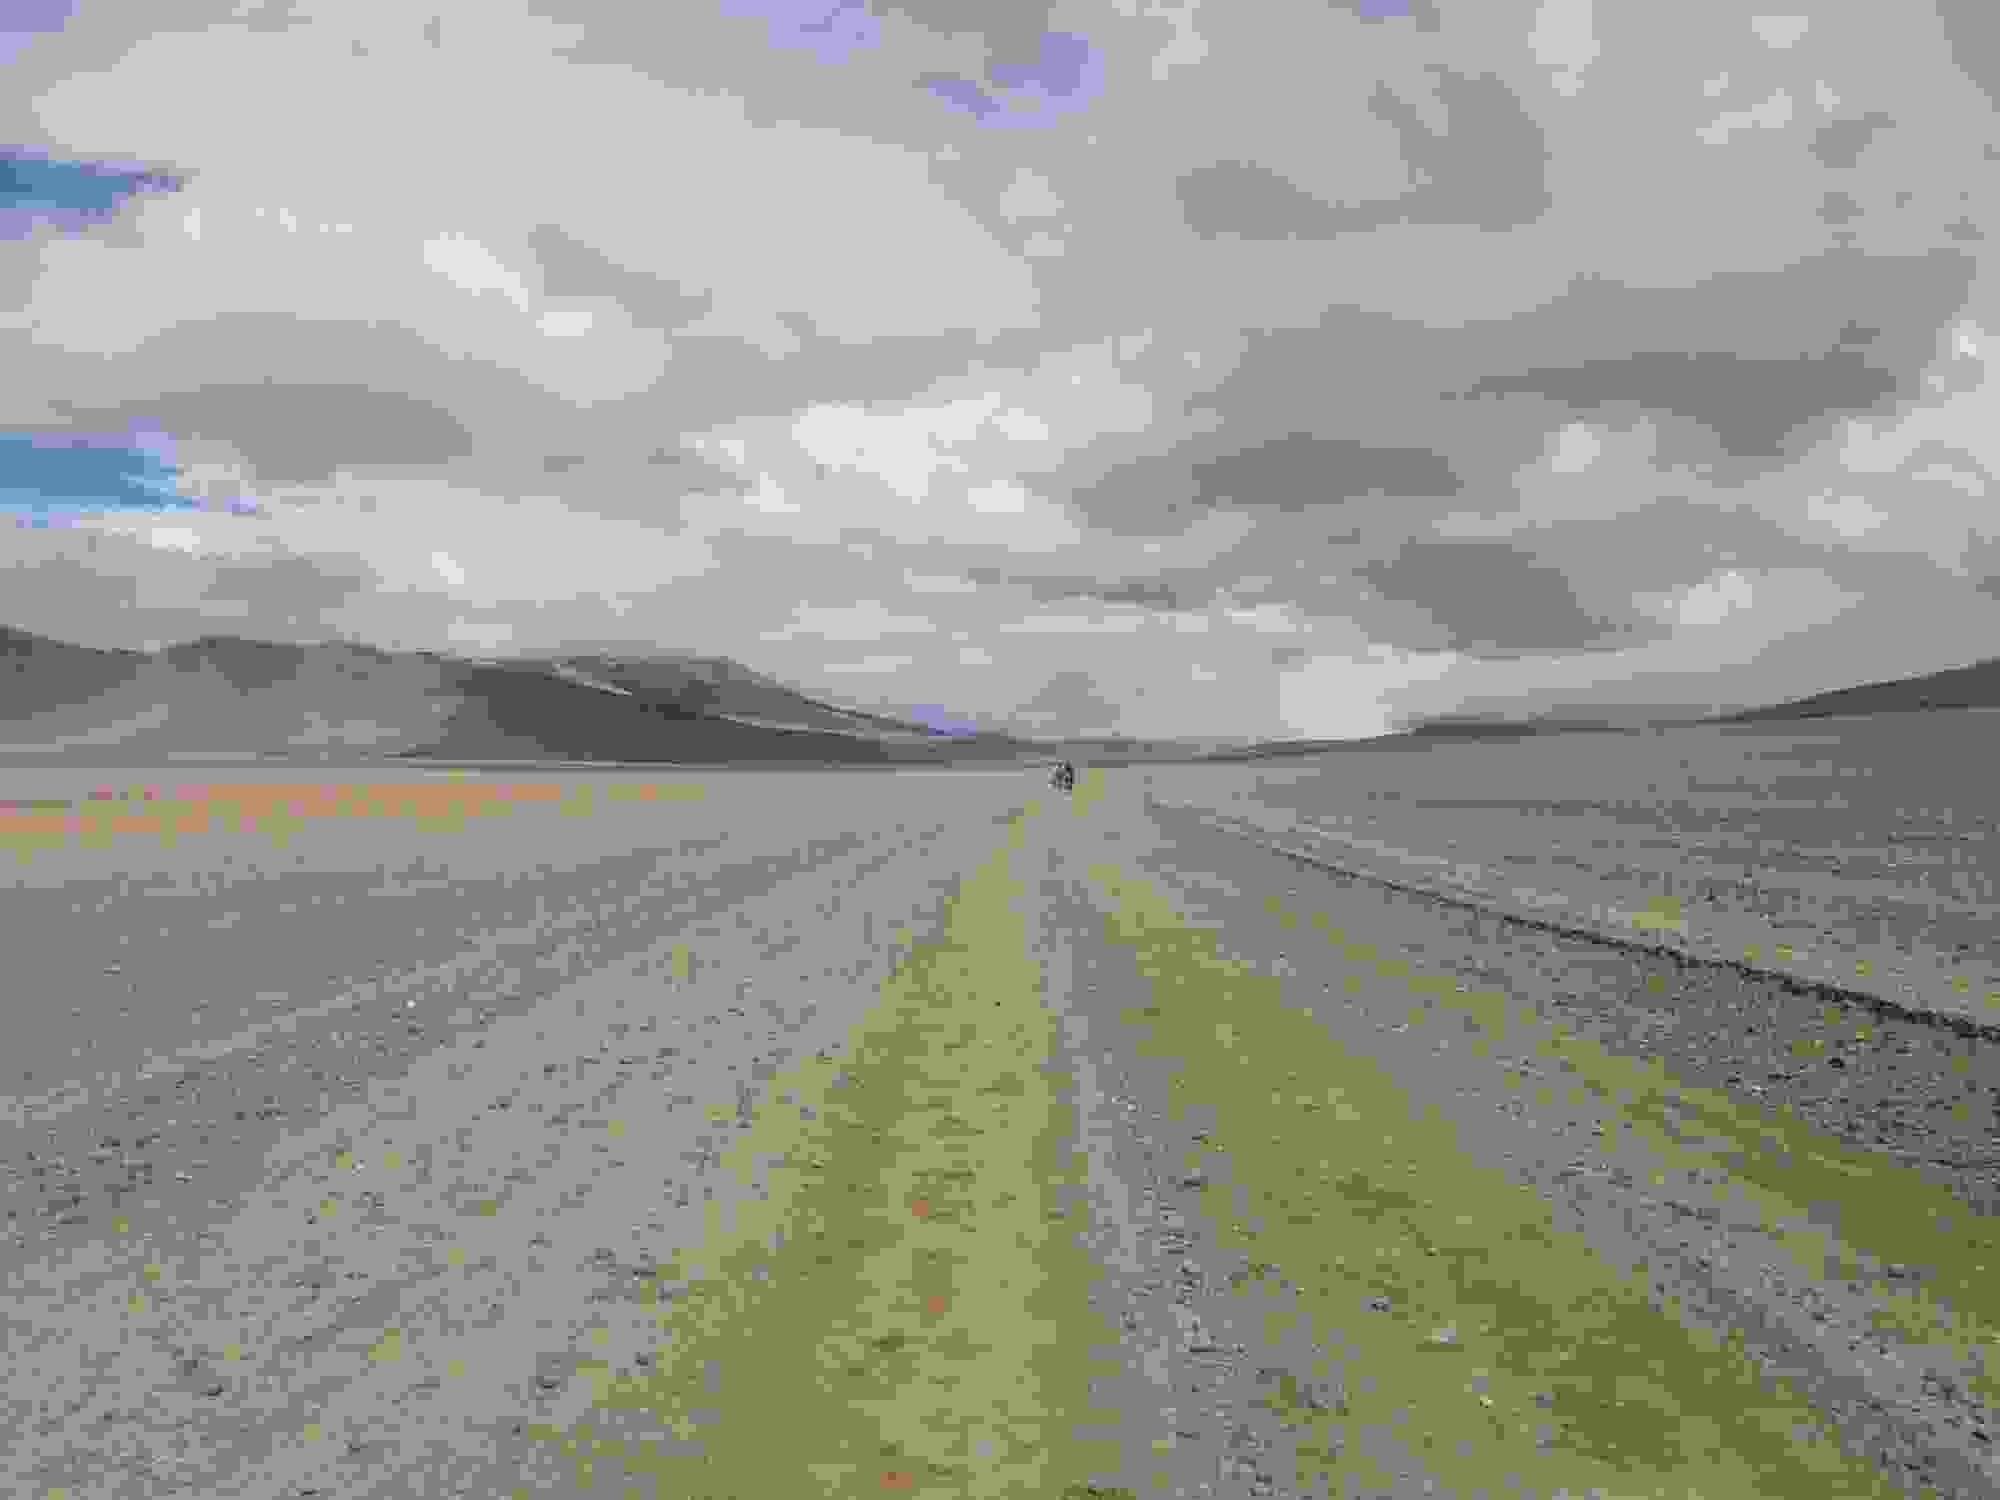
\includegraphics[width=\mywidth]{../wp-content/uploads/2015/04/wpid-wp-1427988827948.jpg} } 
 \newline
 Petit passage sous la grêle et on arrive enfin à l'Arbol de Piedra. \newline
 \newline
\centerline{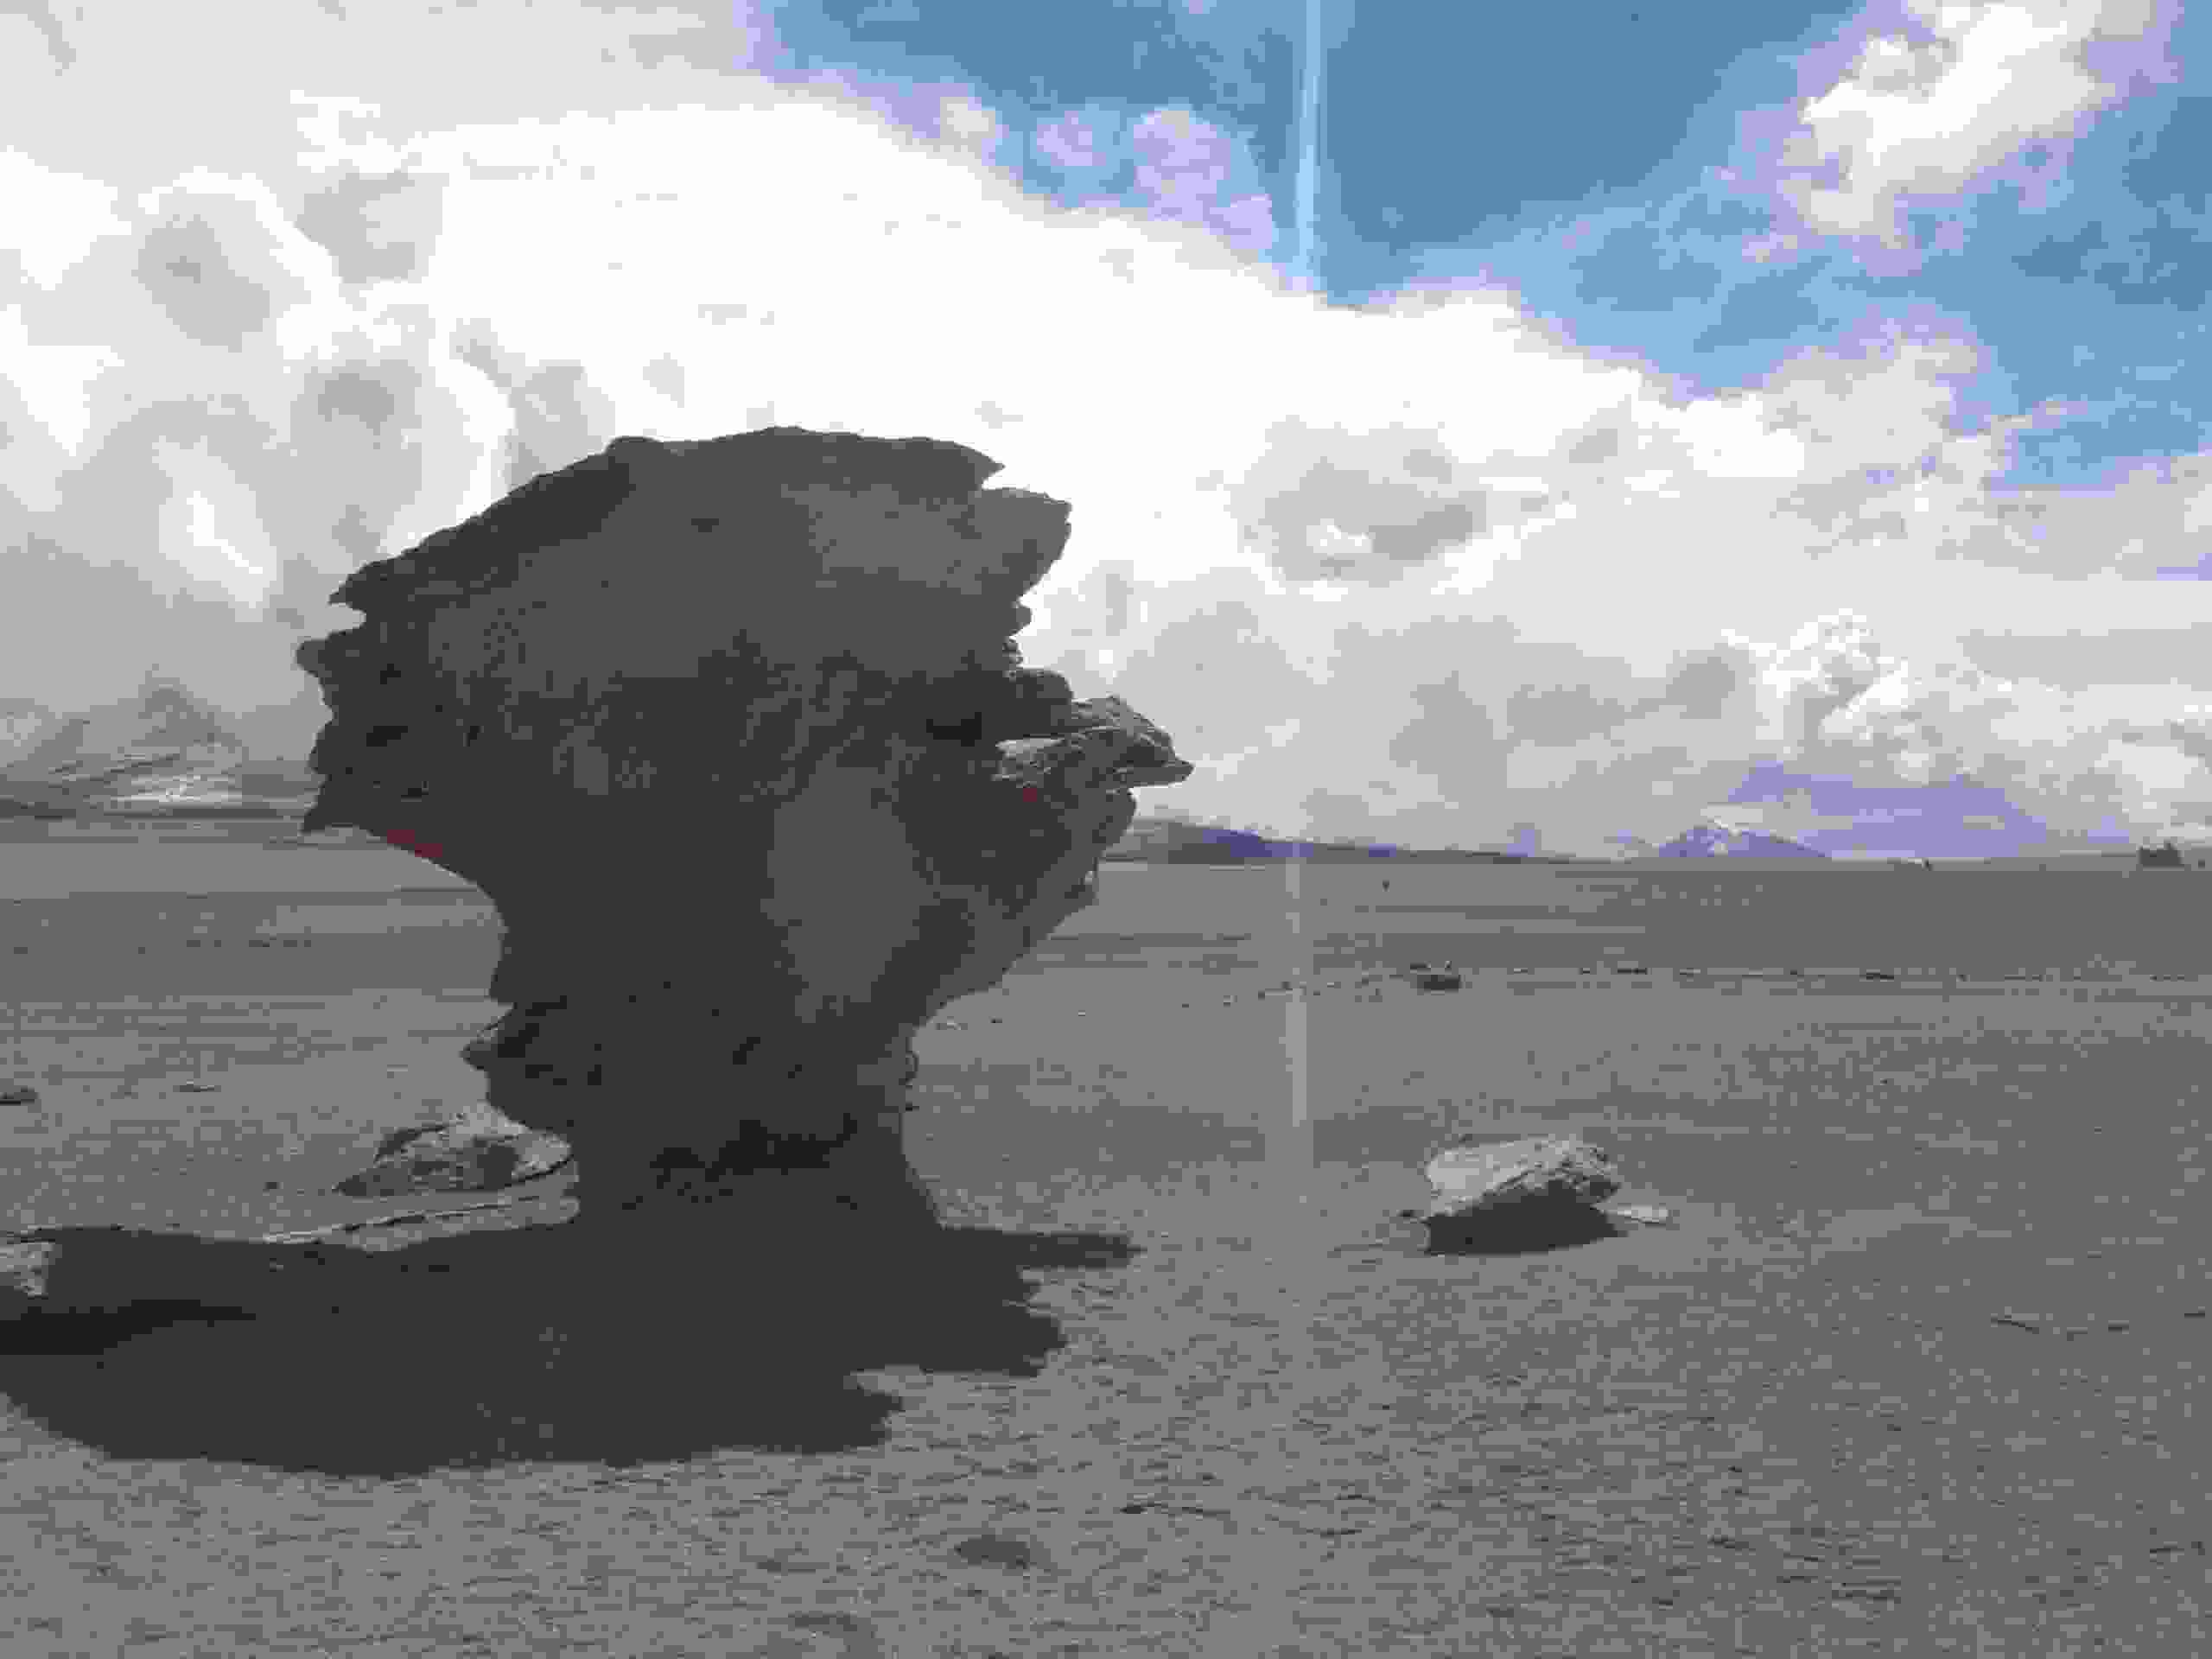
\includegraphics[width=\mywidth]{../wp-content/uploads/2015/04/wpid-wp-1427985000520.jpg} } 
 \newline
 \newline
\centerline{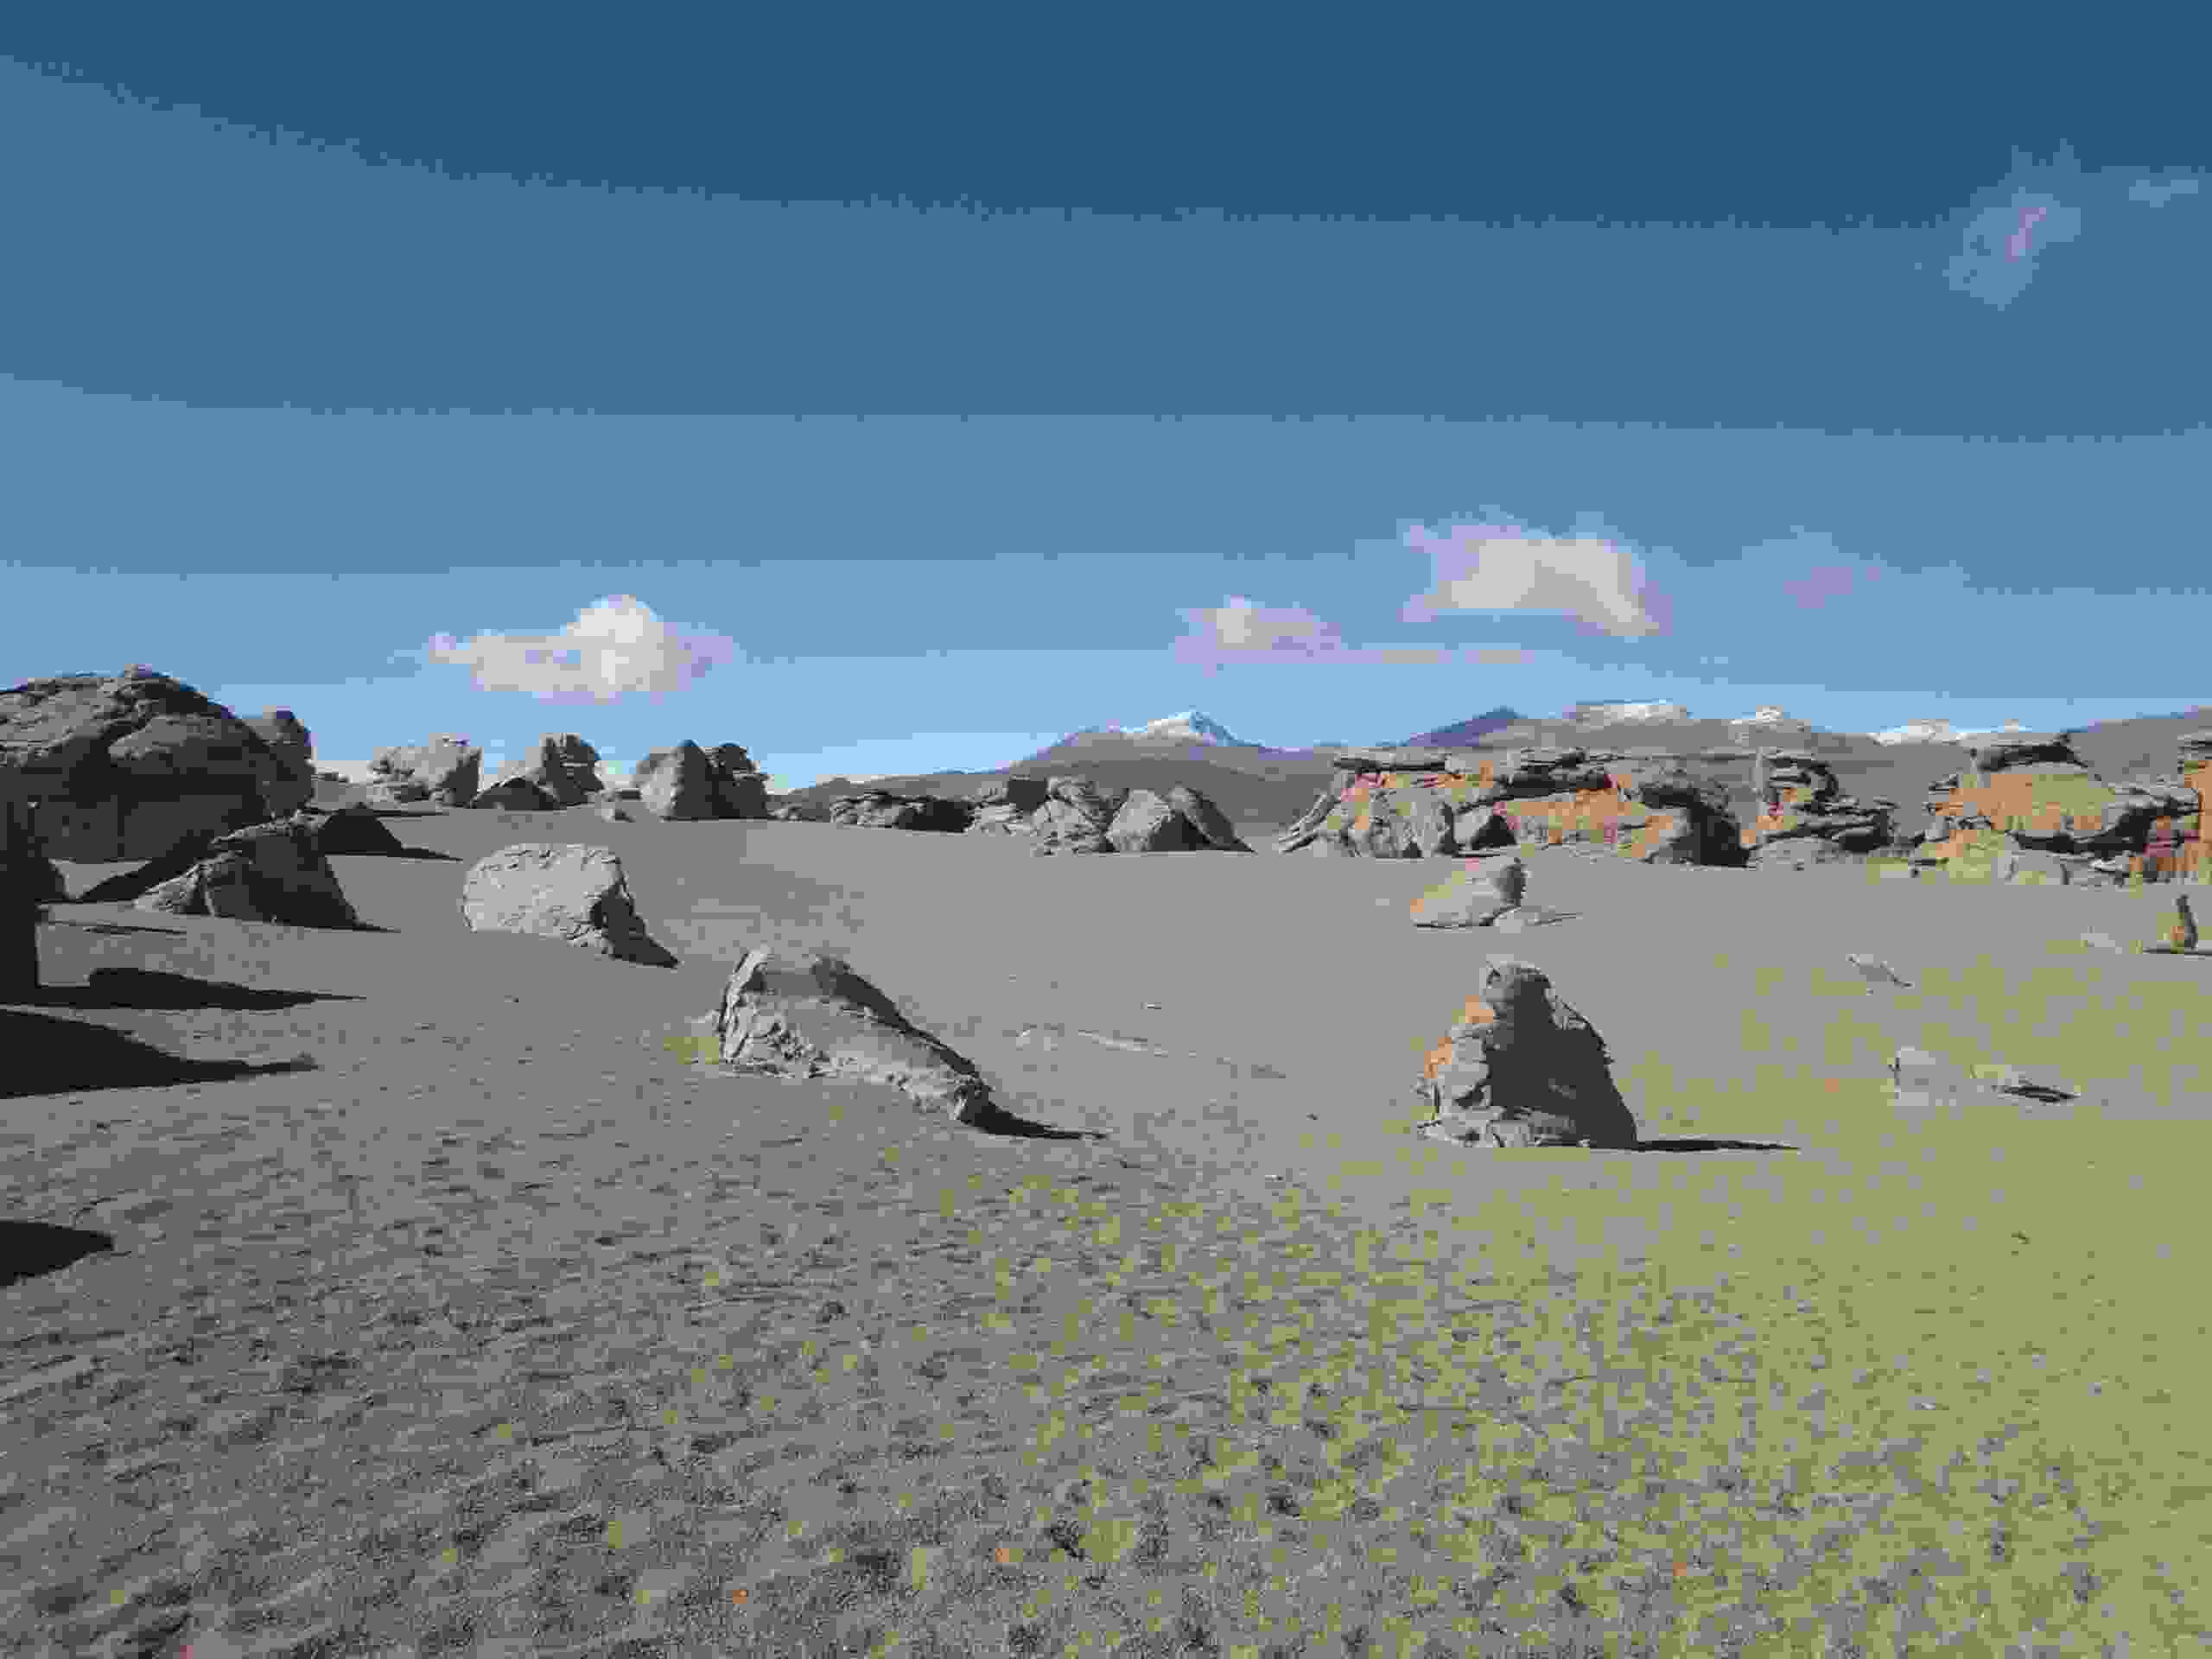
\includegraphics[width=\mywidth]{../wp-content/uploads/2015/04/wpid-wp-1427985029857.jpg} } 
 \newline
 Bivouac très froid à 4600m. \newline
 \newline
\centerline{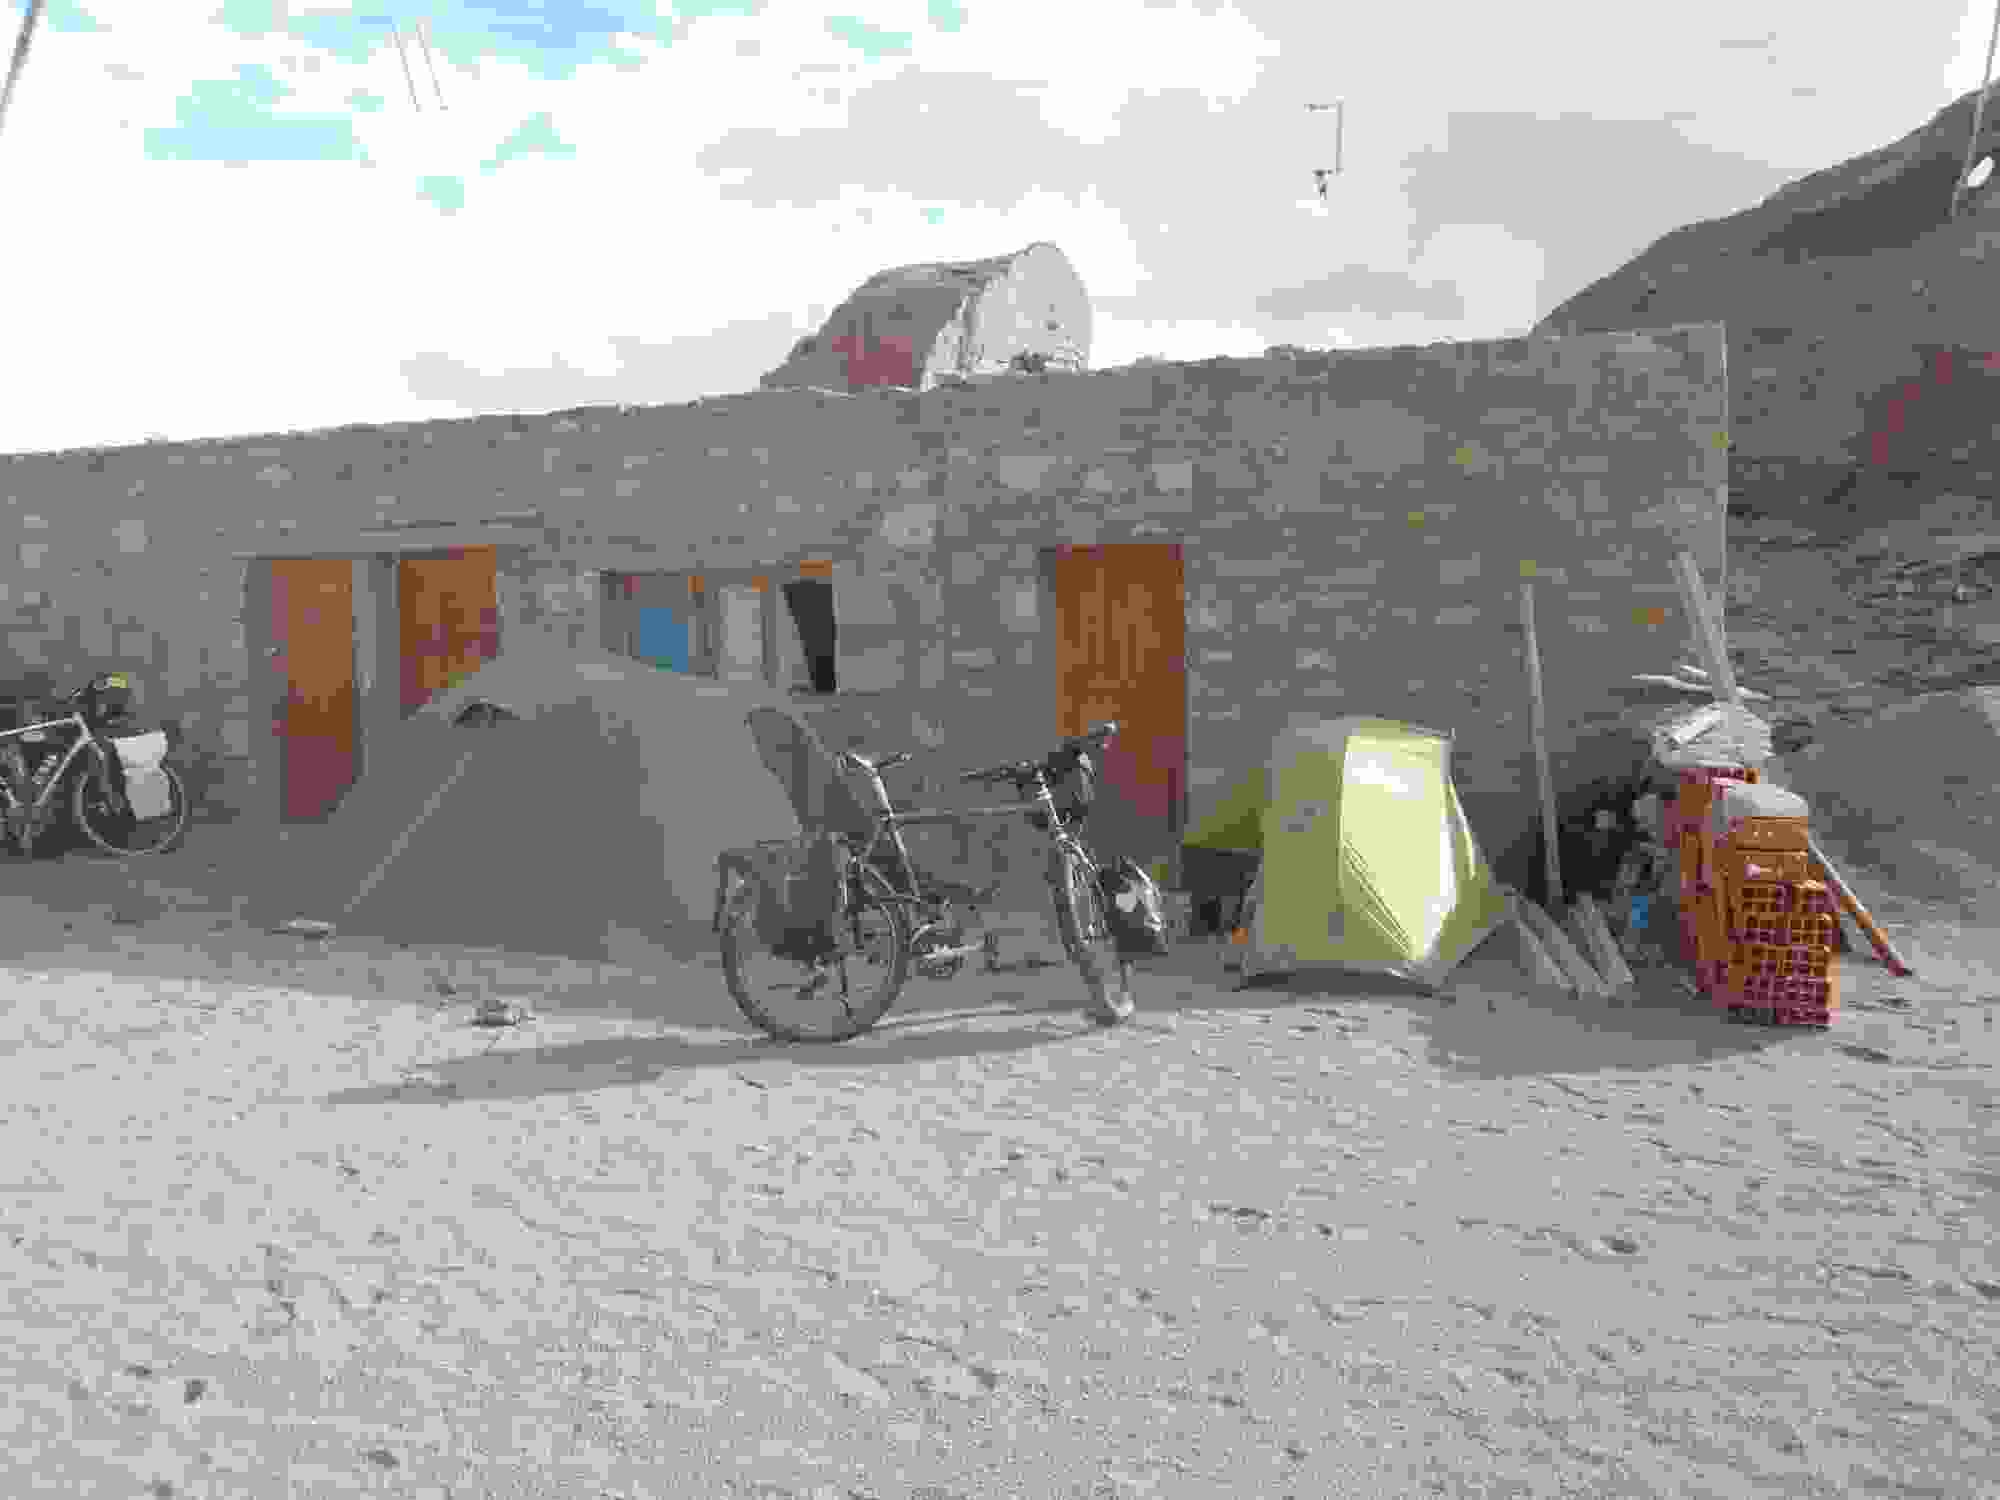
\includegraphics[width=\mywidth]{../wp-content/uploads/2015/04/wpid-wp-1427988855397.jpg} } 
 \newline
 6e jour : \newline
 Le temps s'améliore mais toujours le vent de face. \newline
 \newline
\centerline{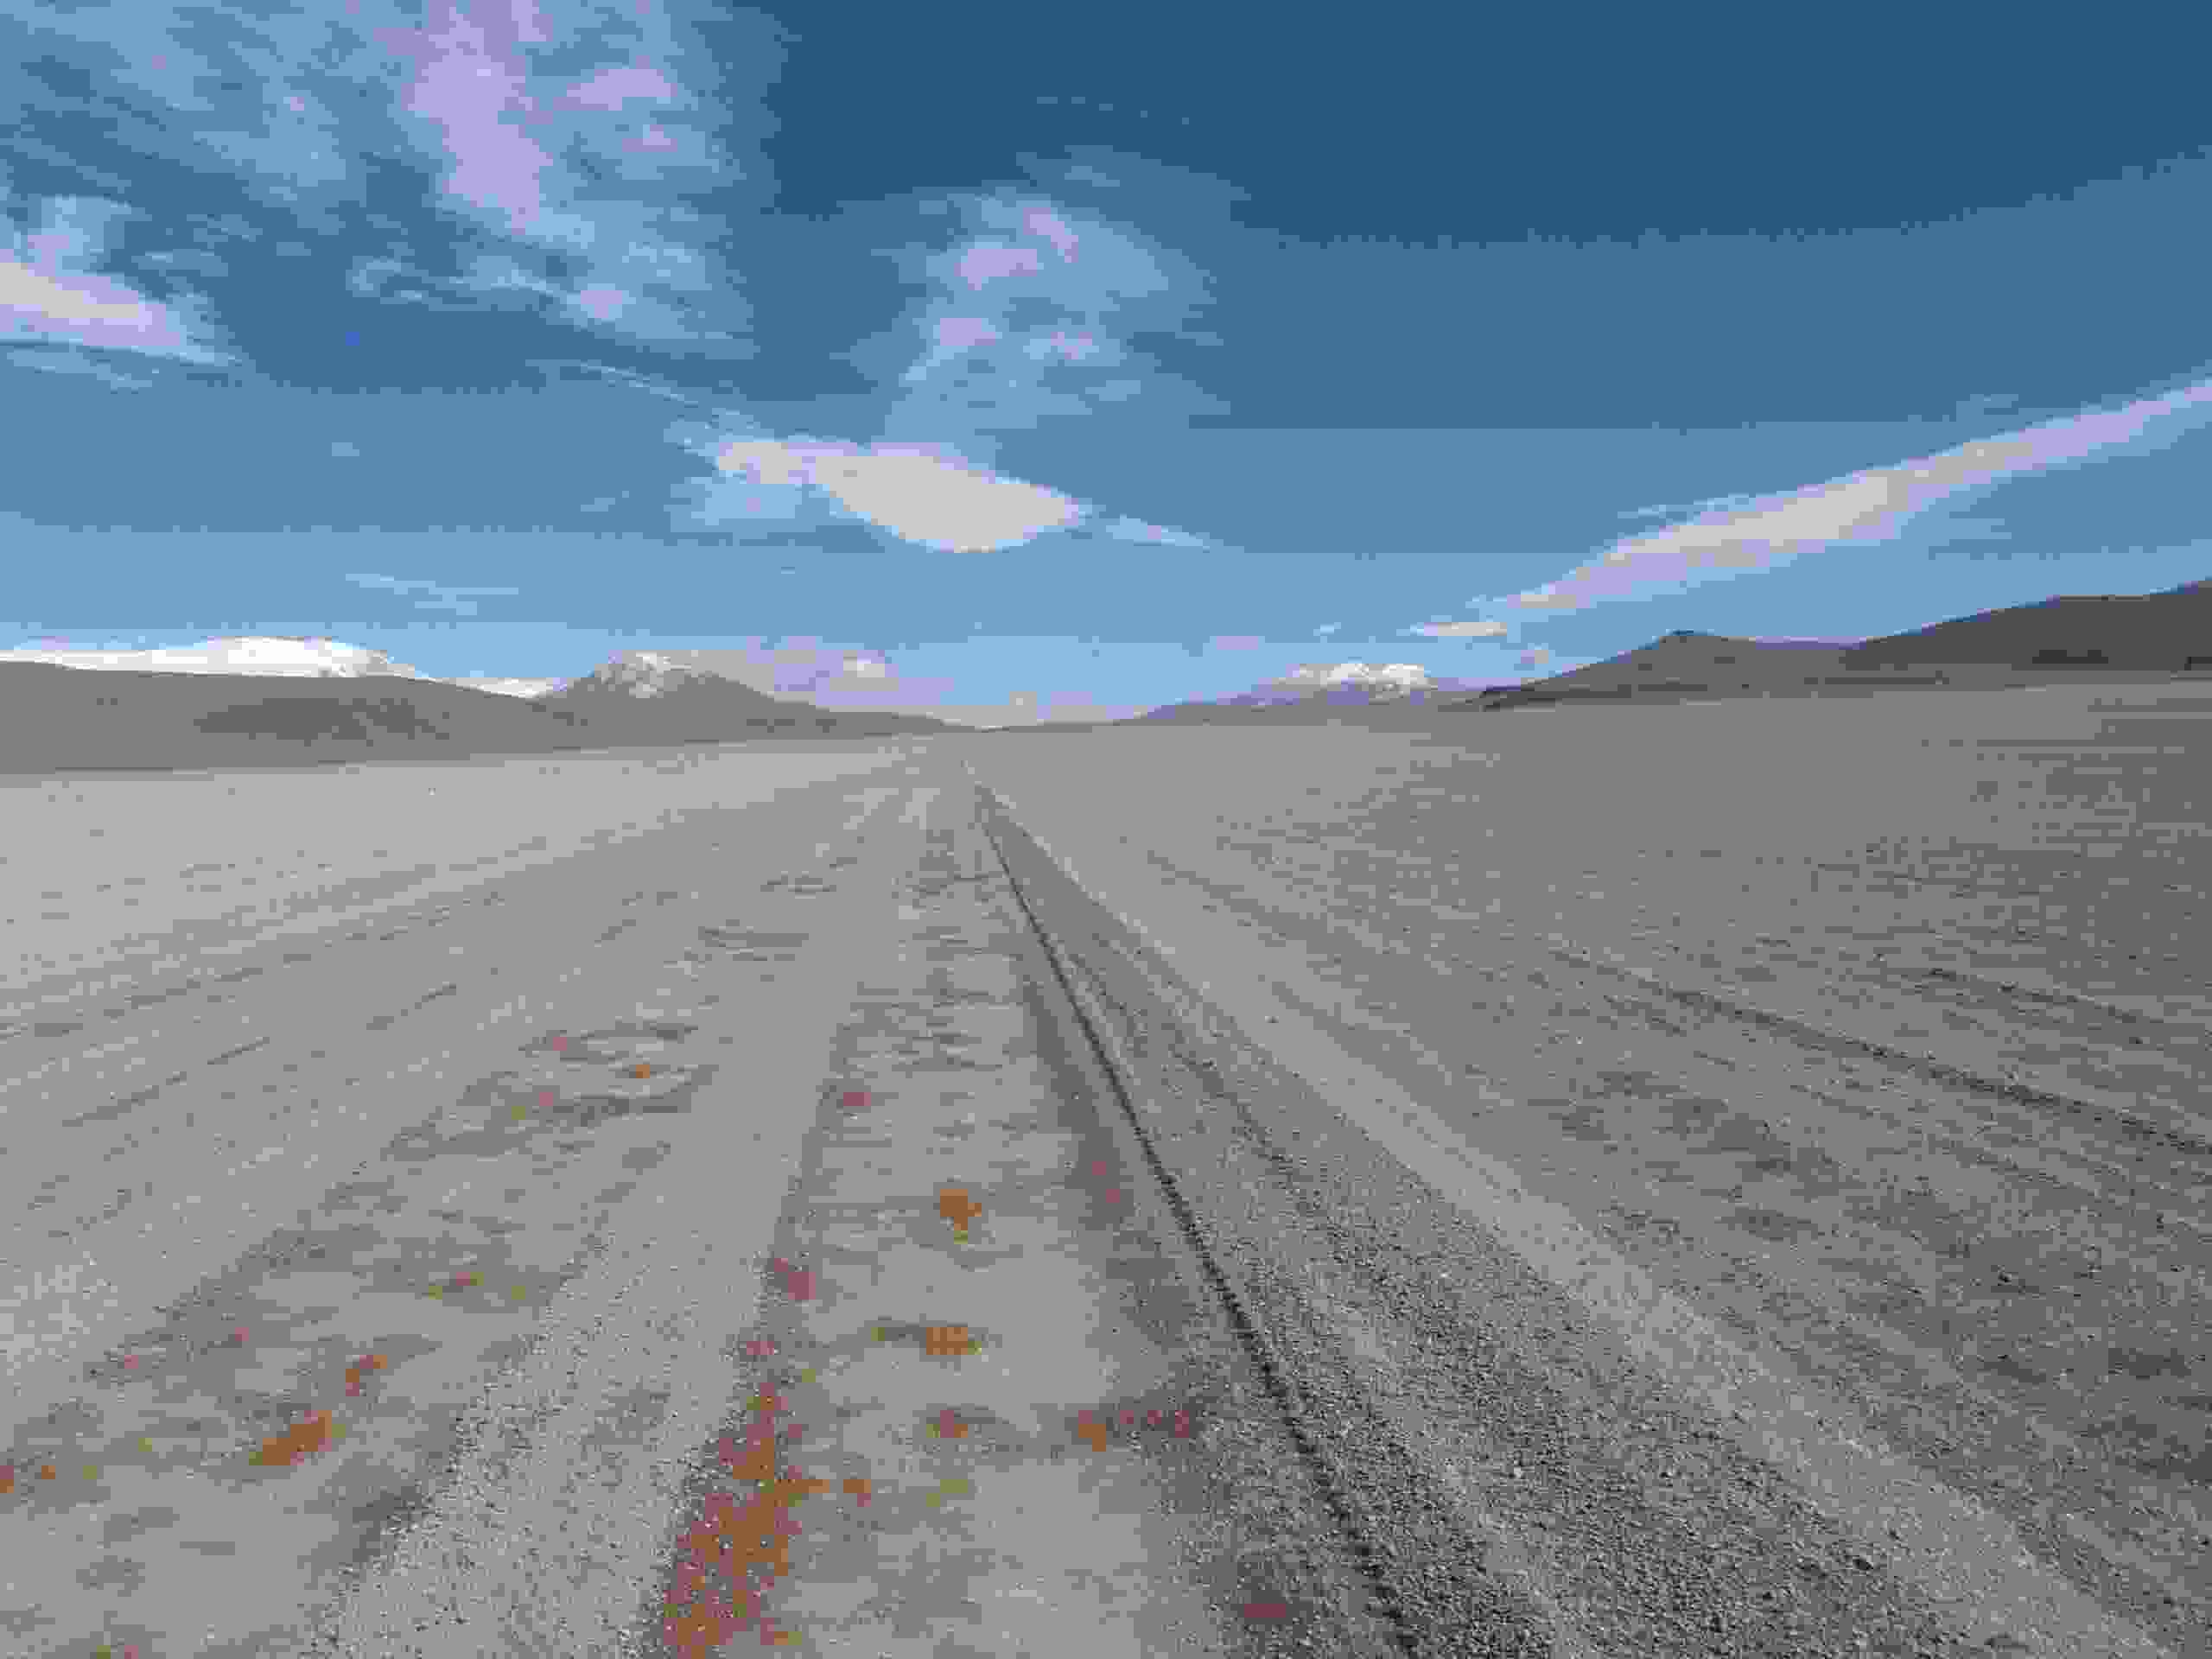
\includegraphics[width=\mywidth]{../wp-content/uploads/2015/04/wpid-wp-1427985056062.jpg} } 
 \newline
 Pique nique à l'abri des rochers. \newline
 \newline
\centerline{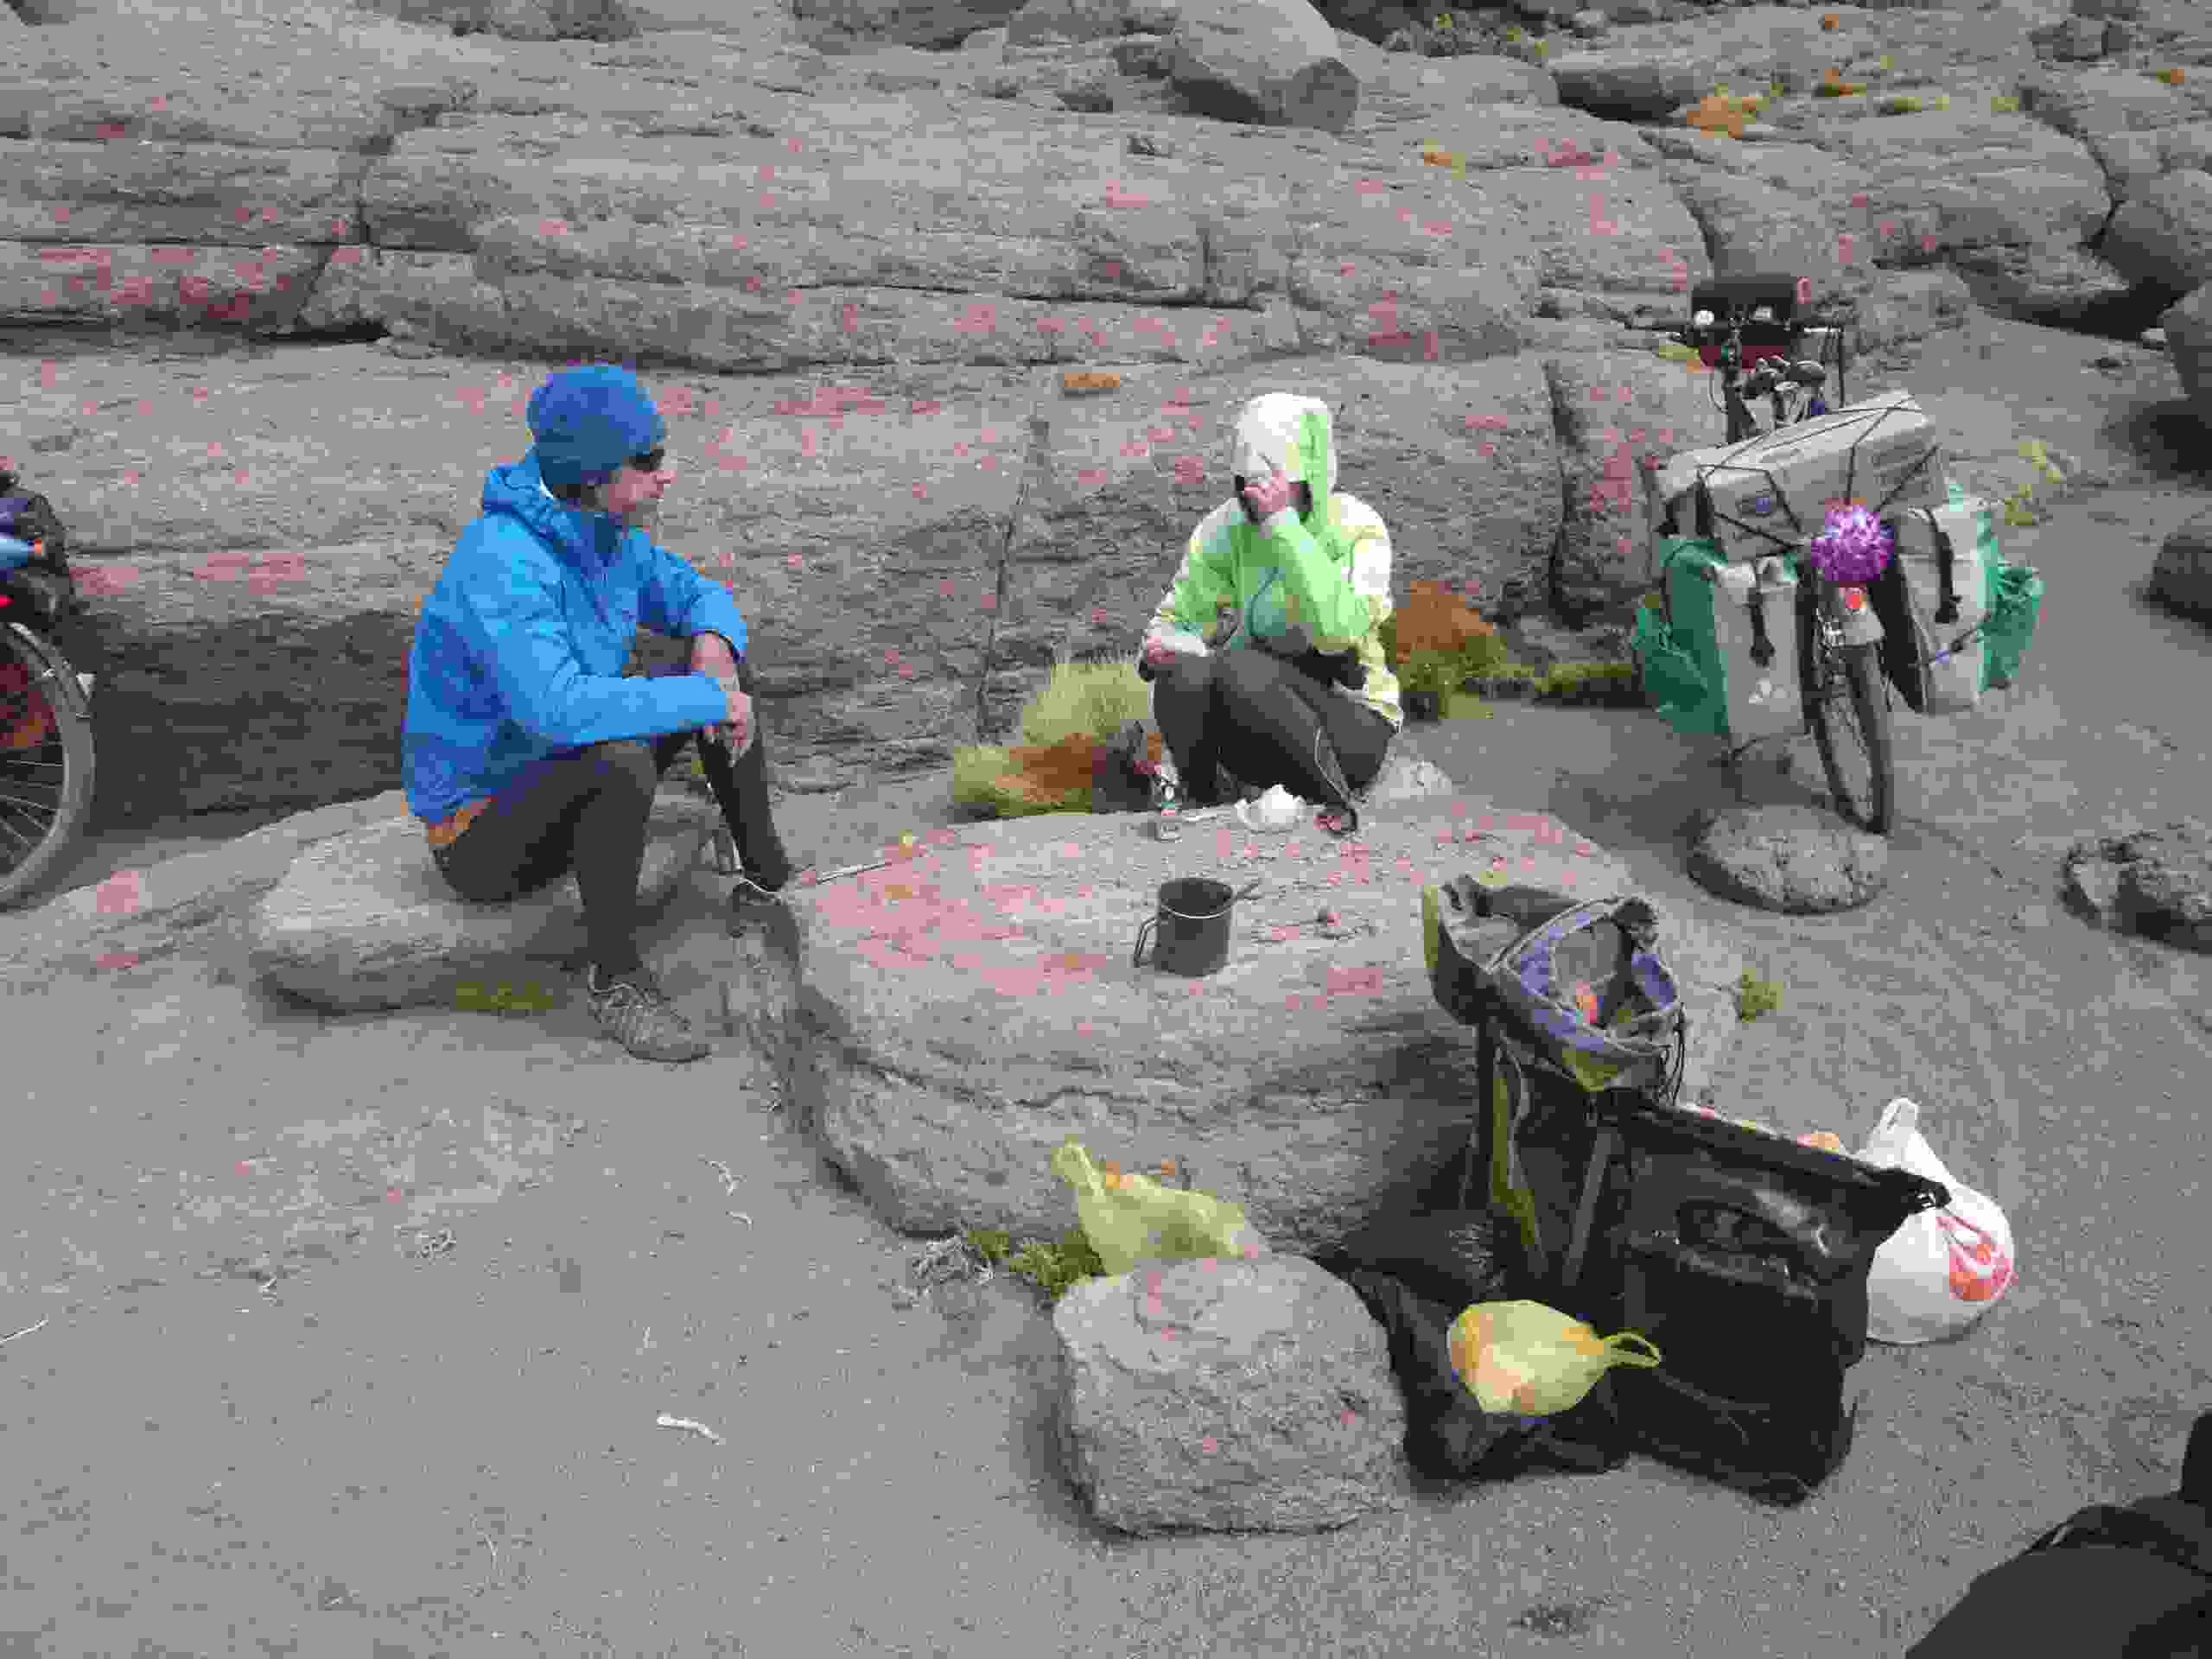
\includegraphics[width=\mywidth]{../wp-content/uploads/2015/04/wpid-wp-1427985094336.jpg} } 
 \newline
 Une mousse de la région : au toucher c'est dur comme de la pierre. \newline
 \newline
\centerline{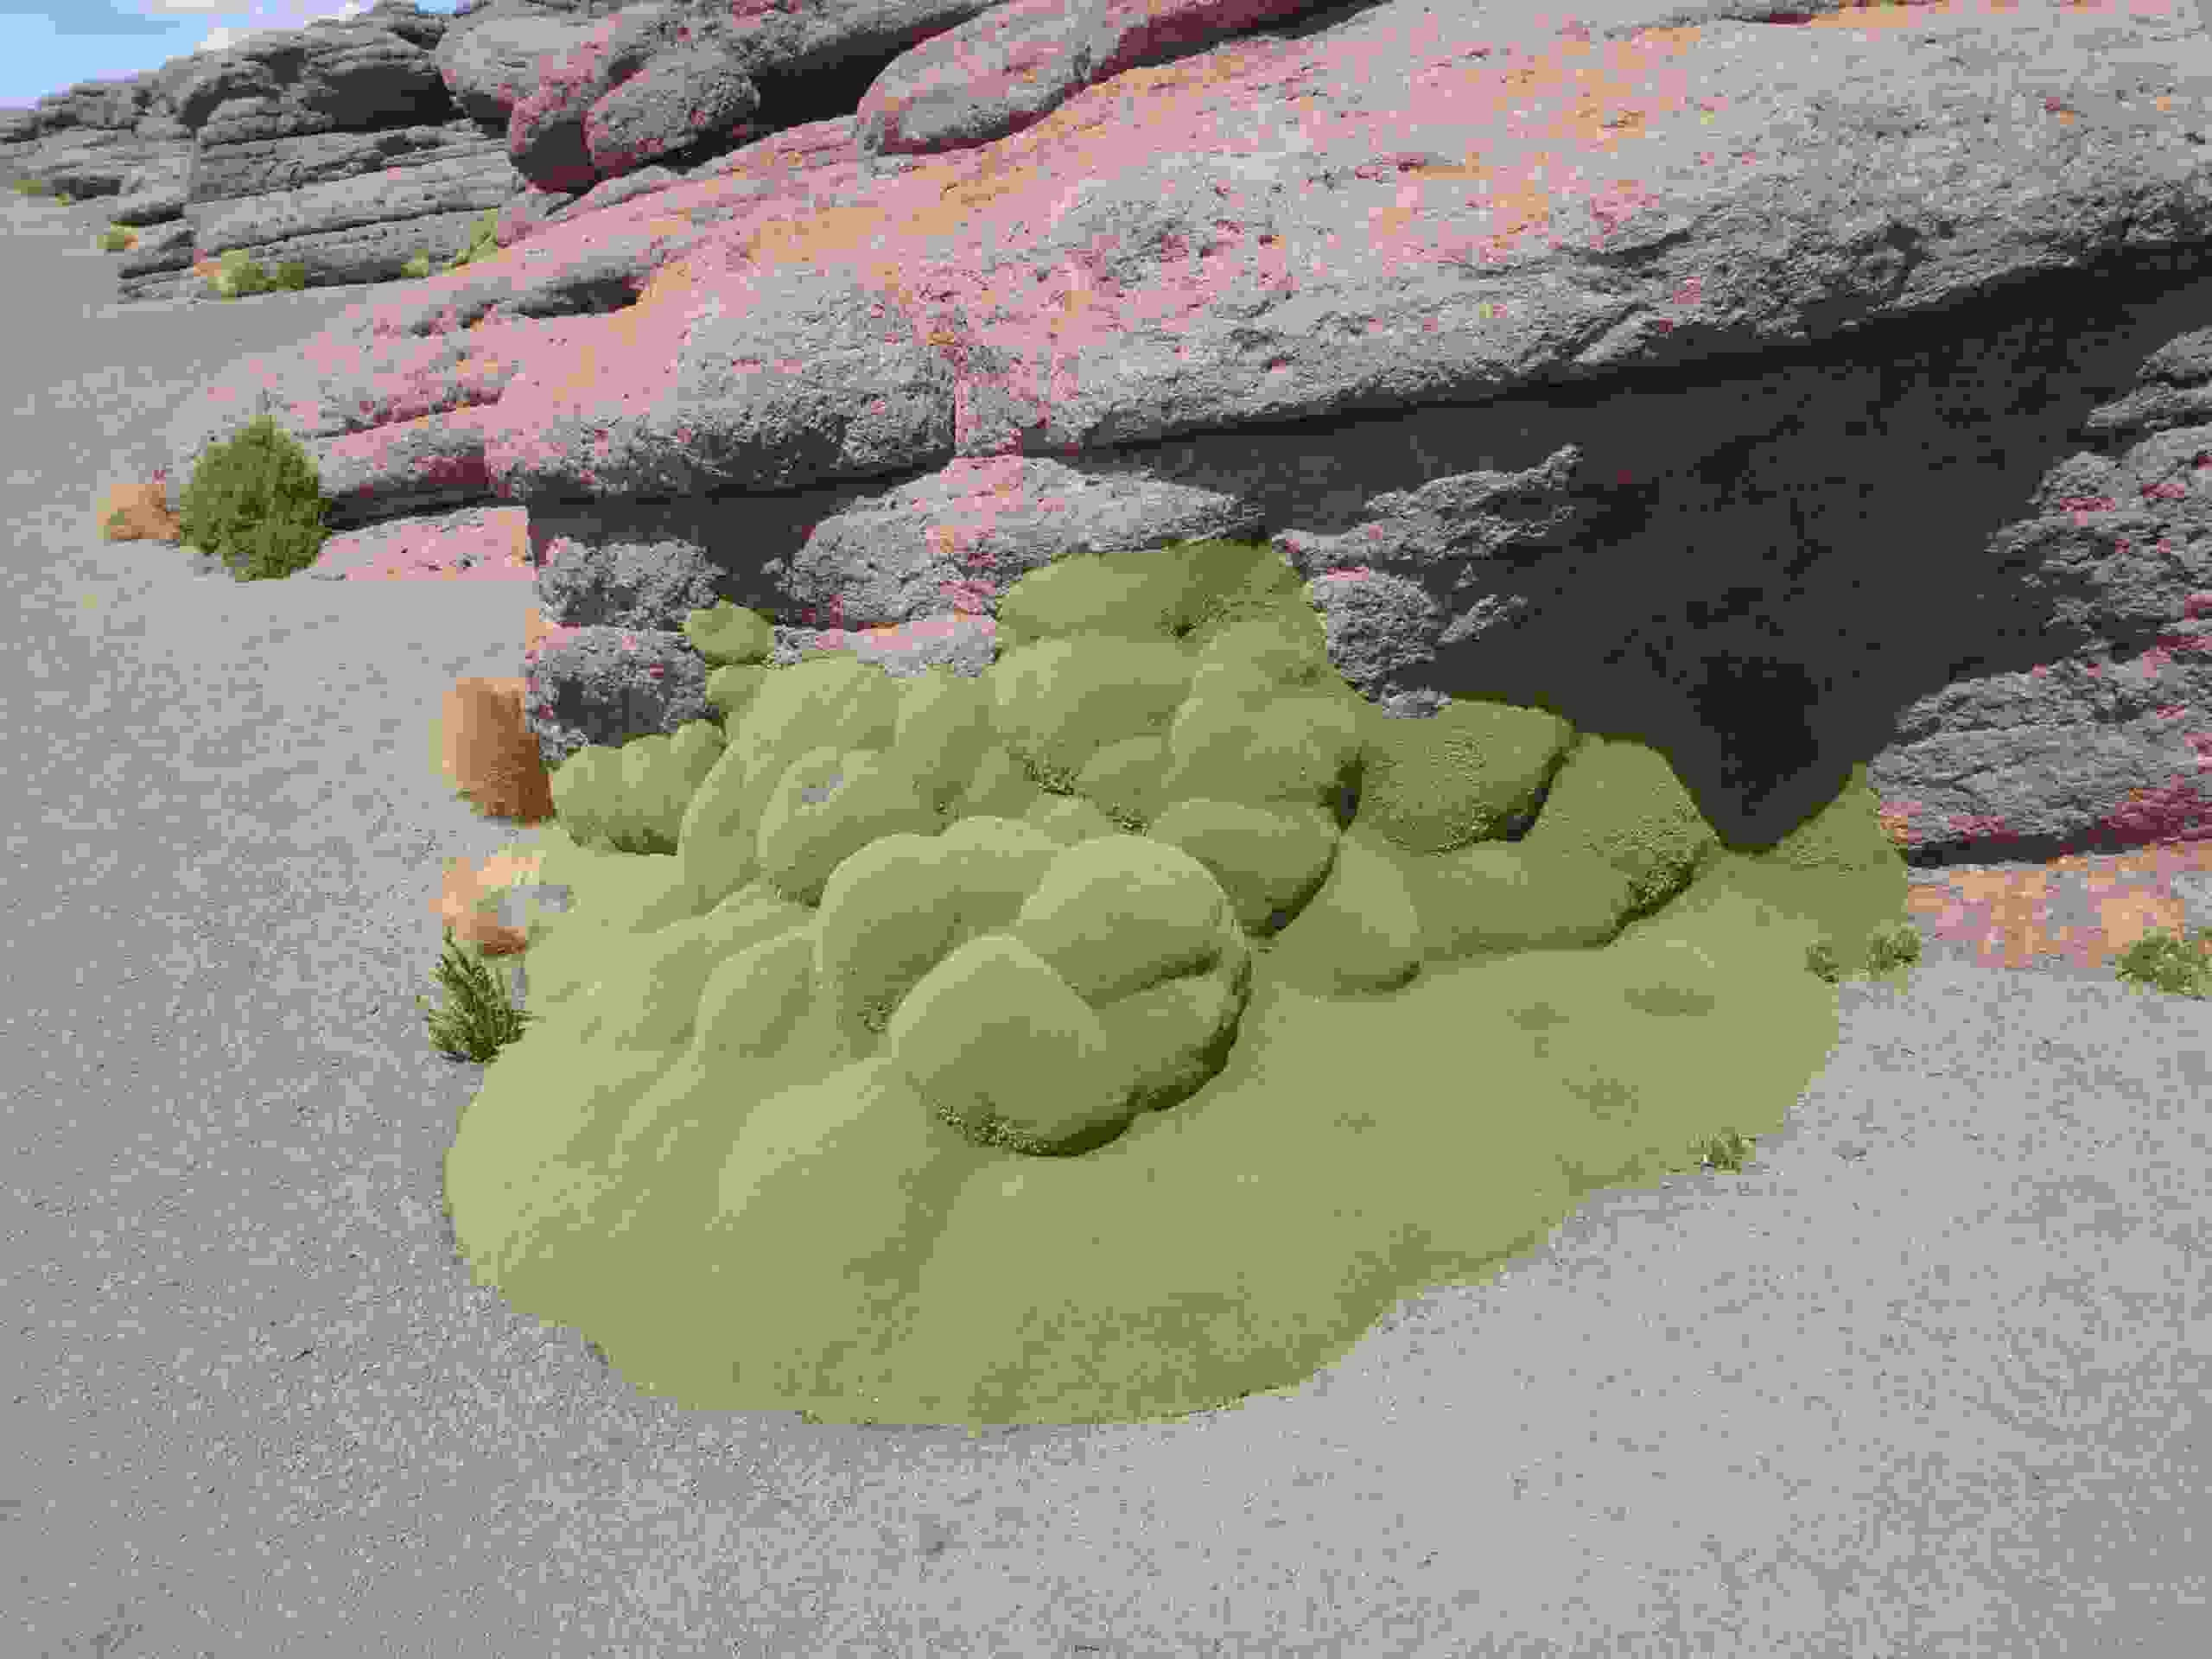
\includegraphics[width=\mywidth]{../wp-content/uploads/2015/04/wpid-wp-1427985074703.jpg} } 
 \newline
 La fin de journée est horrible avec le vent froid et dans le sable j'arrive épuisé à l'hôtel del Desierto. \newline
 \newline
\centerline{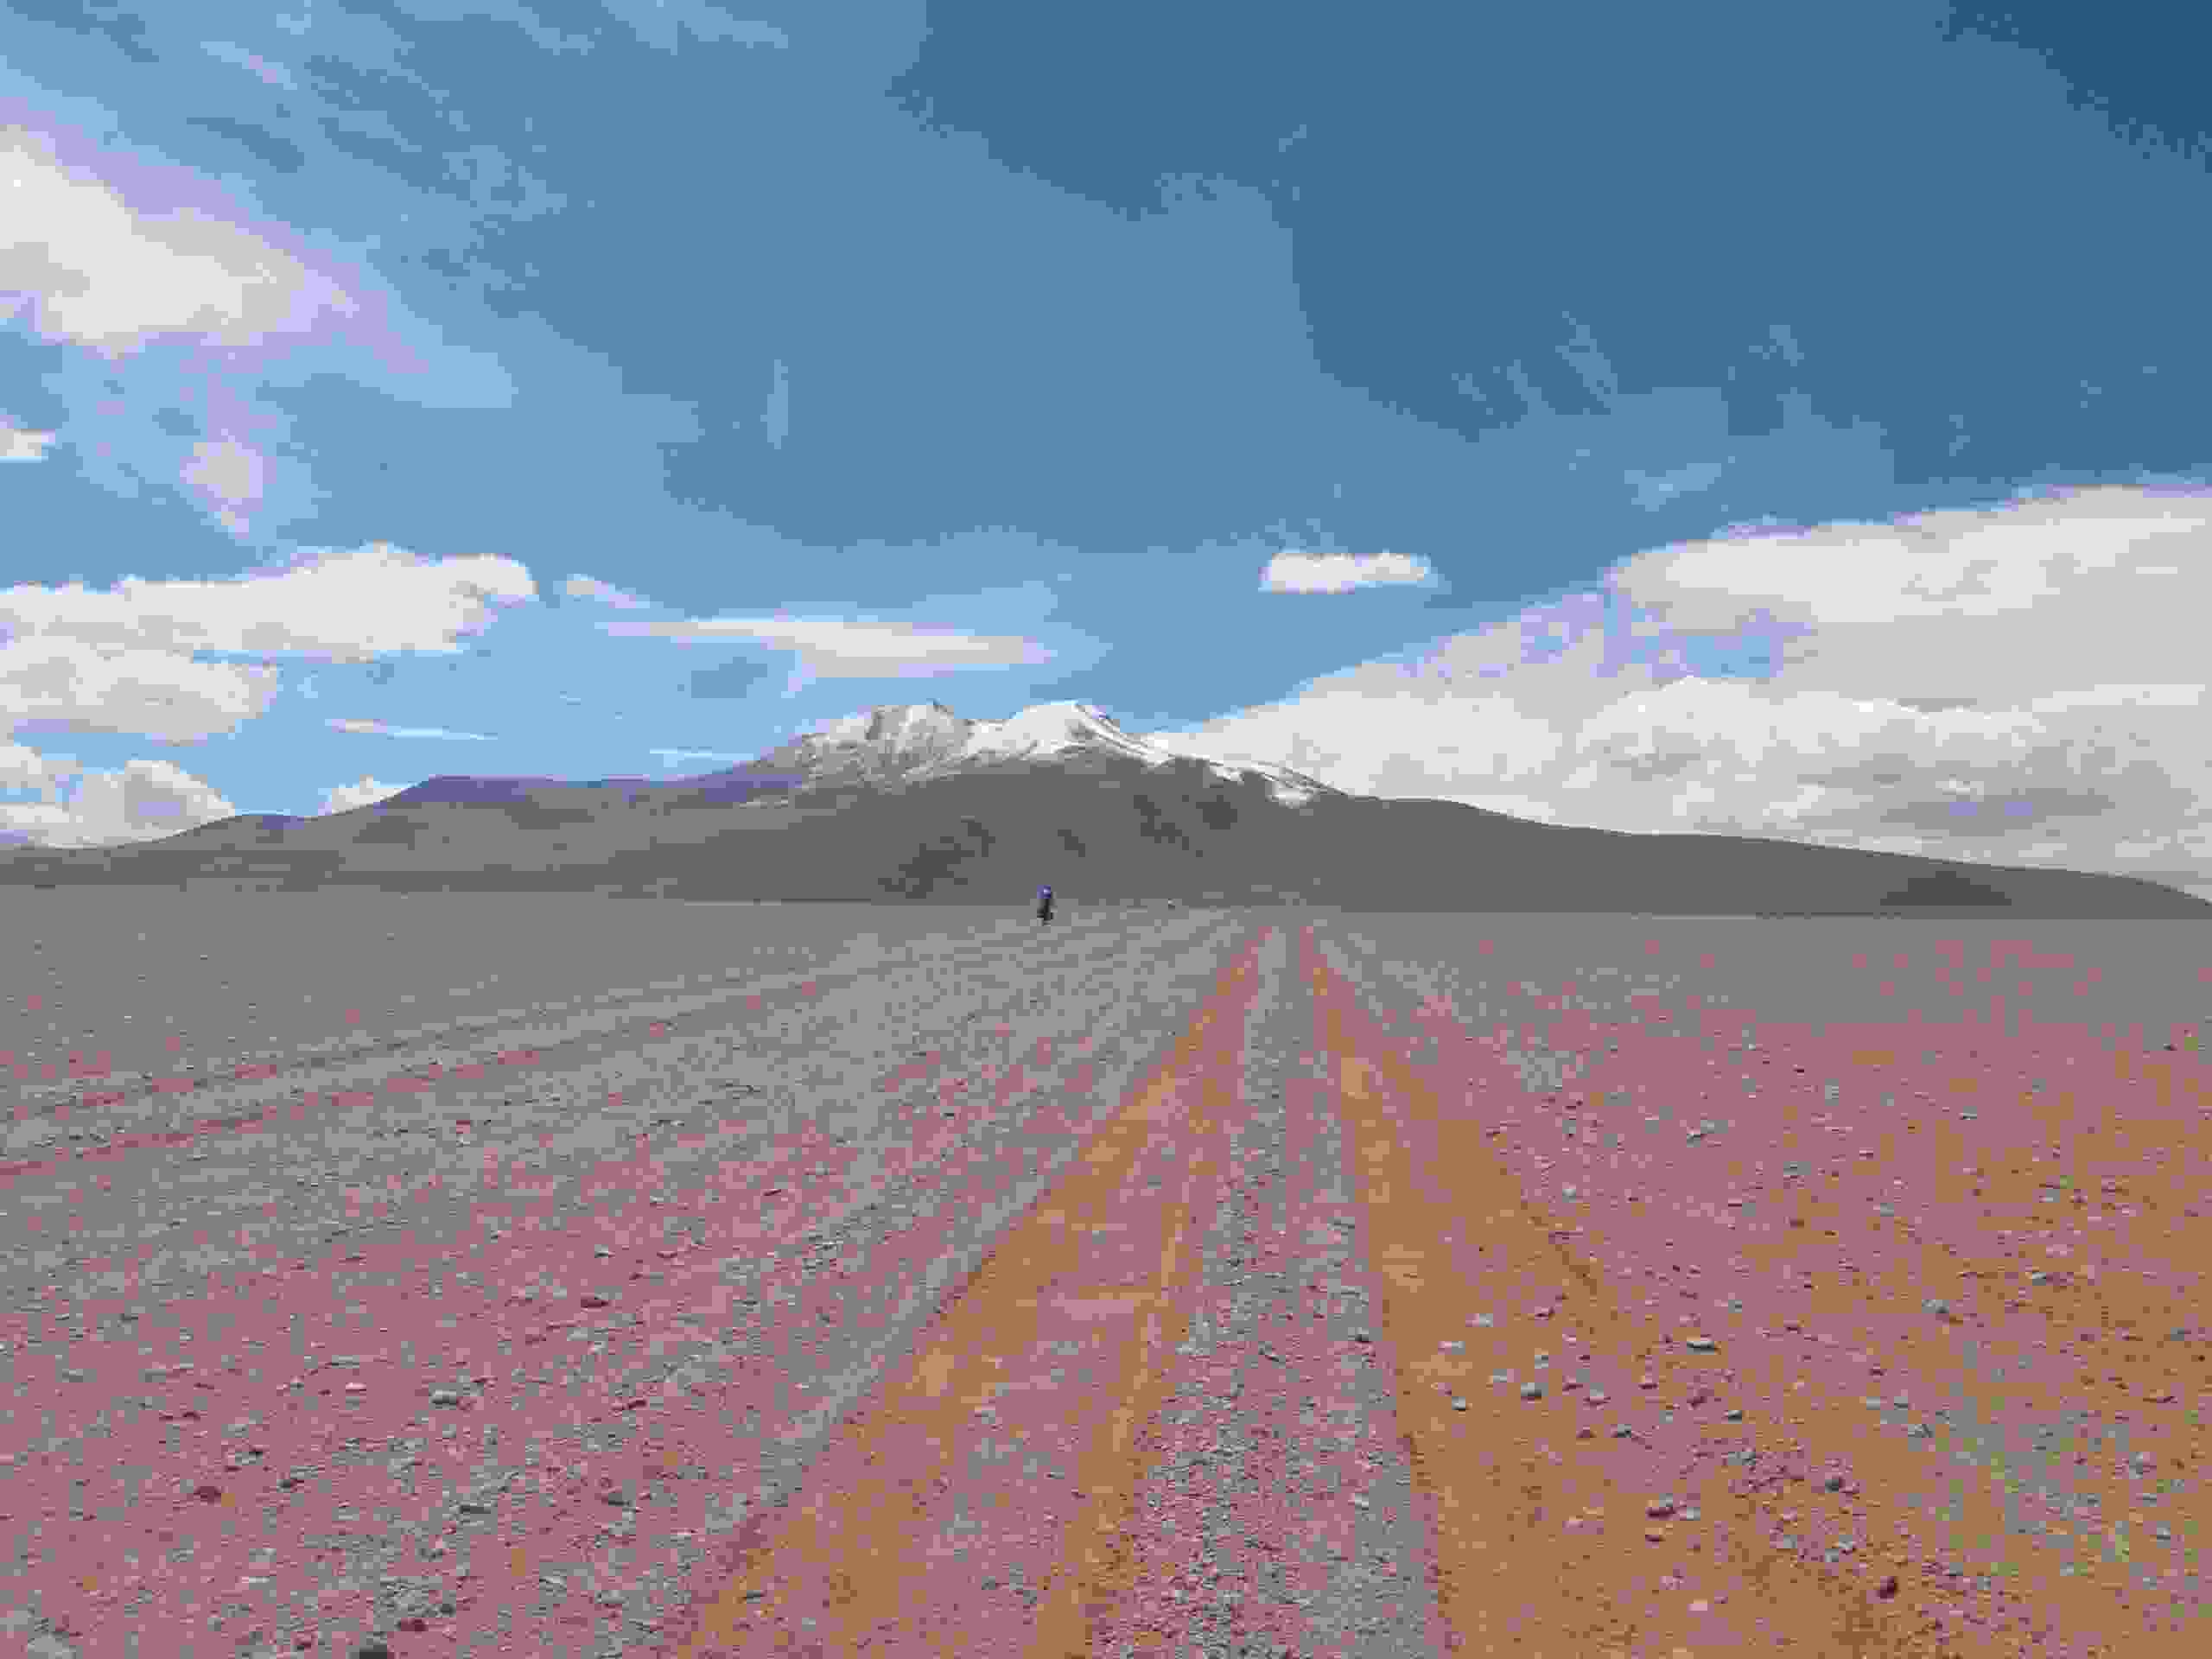
\includegraphics[width=\mywidth]{../wp-content/uploads/2015/04/wpid-wp-1427985137543.jpg} } 
 \newline
 On nous annonce un prix exorbitant de 150 dollars pour la nuit, heureusement on arrive à obtenir le tarif bolivien, environ un tiers du prix. J'avais bien besoin d'un vrai lit pour récupérer. \newline
 \newline
\centerline{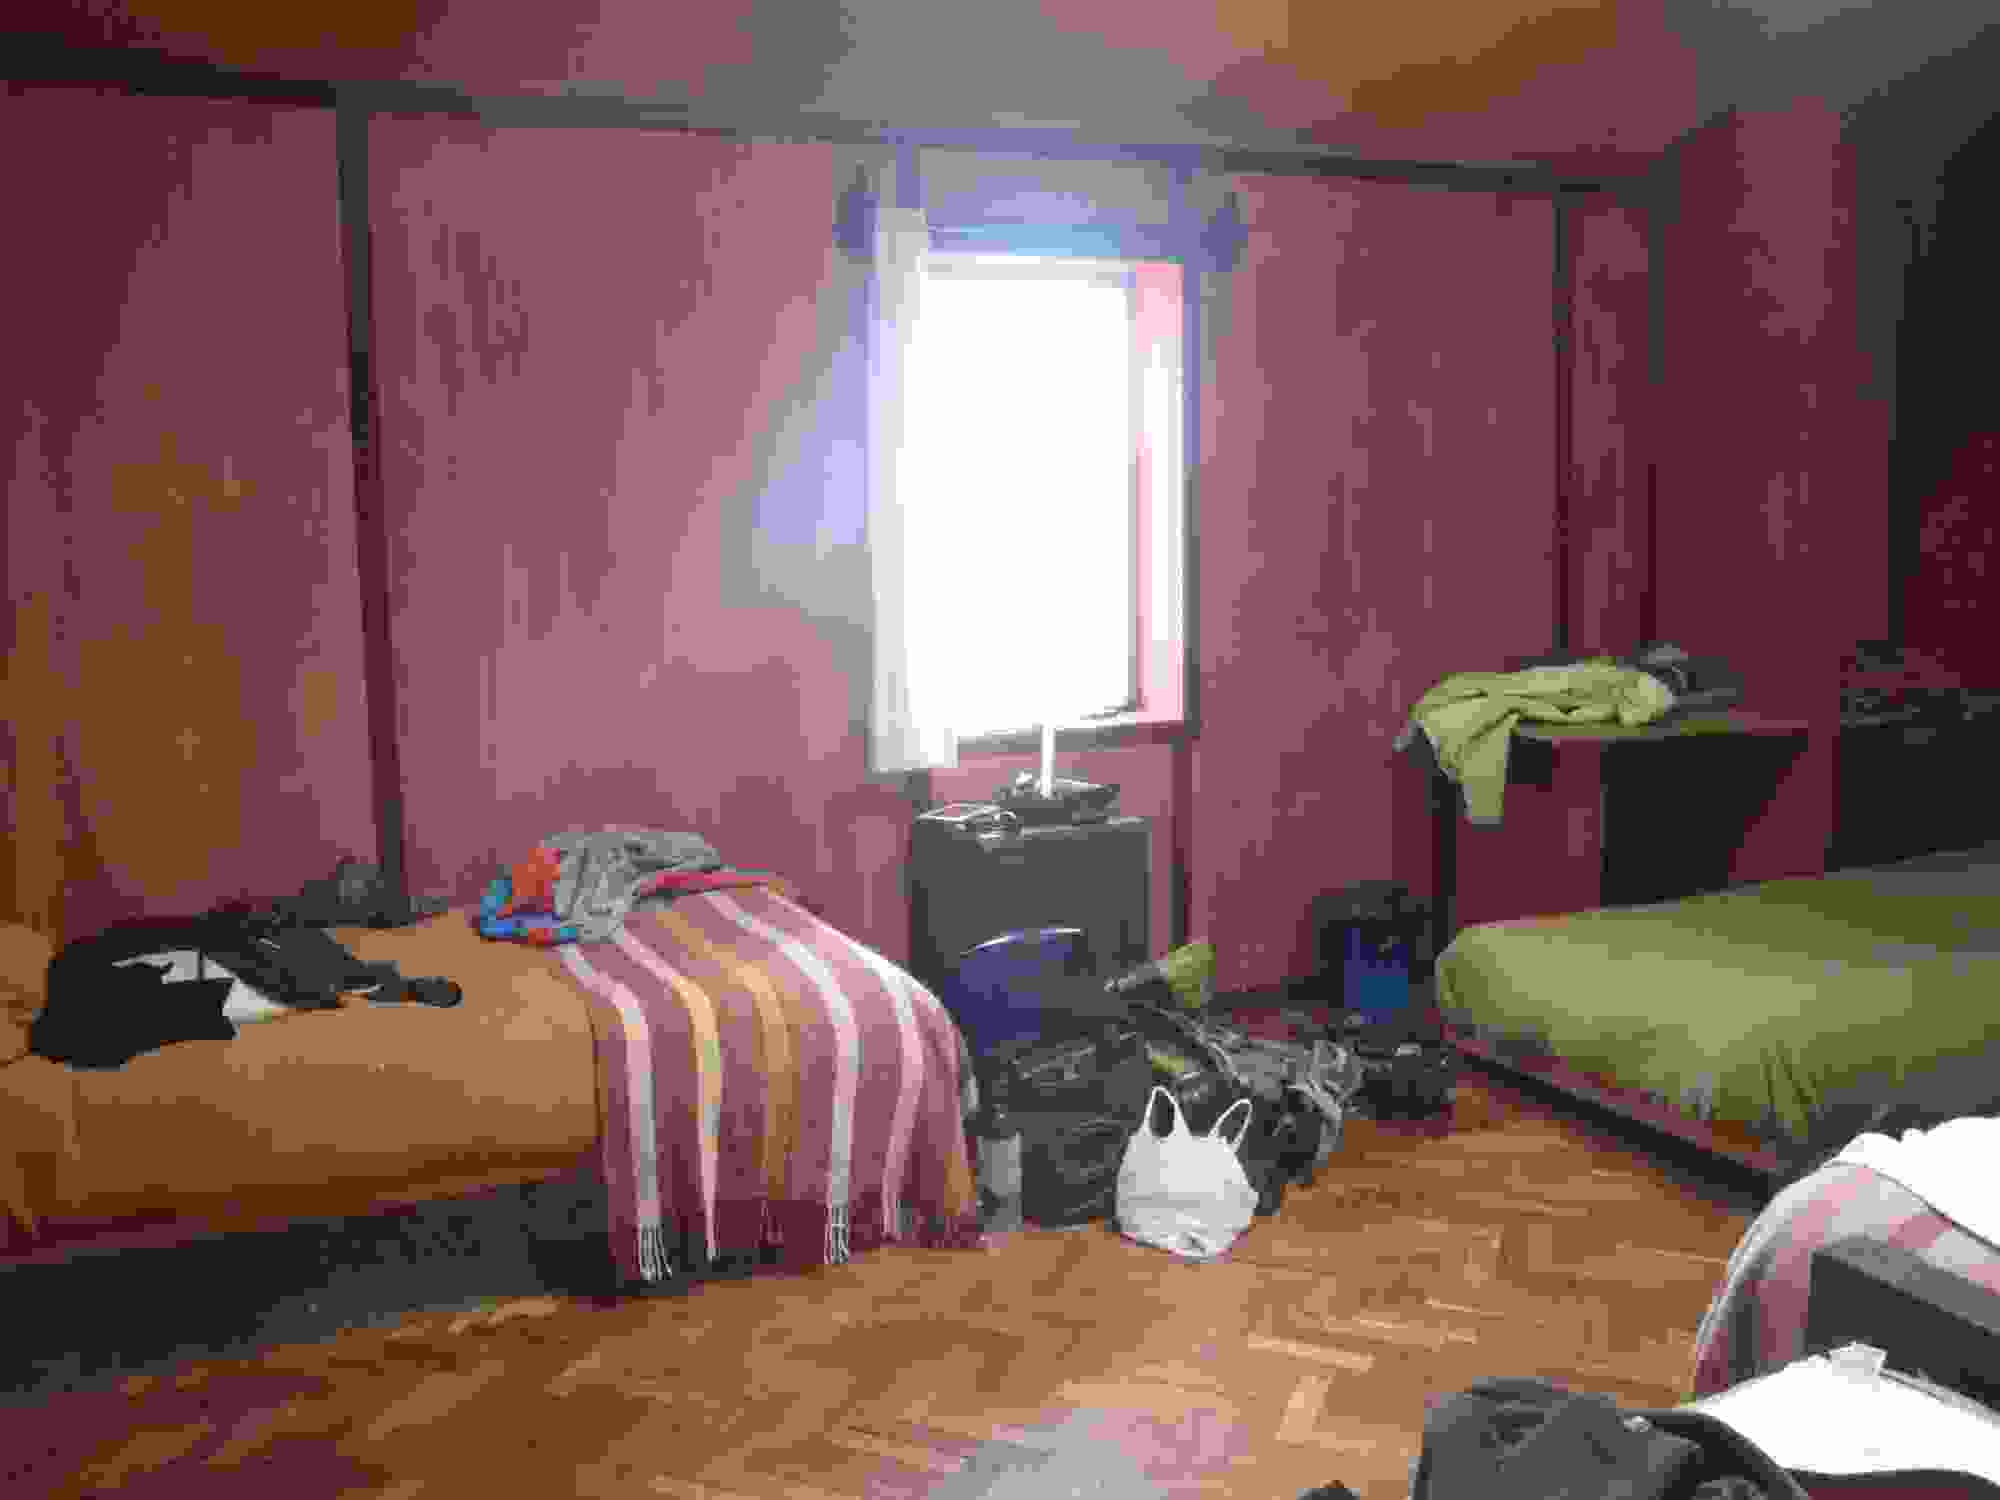
\includegraphics[width=\mywidth]{../wp-content/uploads/2015/04/wpid-wp-1427989235491.jpg} } 
 \newline
 7e jour : \newline
 Première partie encore difficile et dans le vent mais grand ciel bleu : bon pour le moral. \newline
 \newline
\centerline{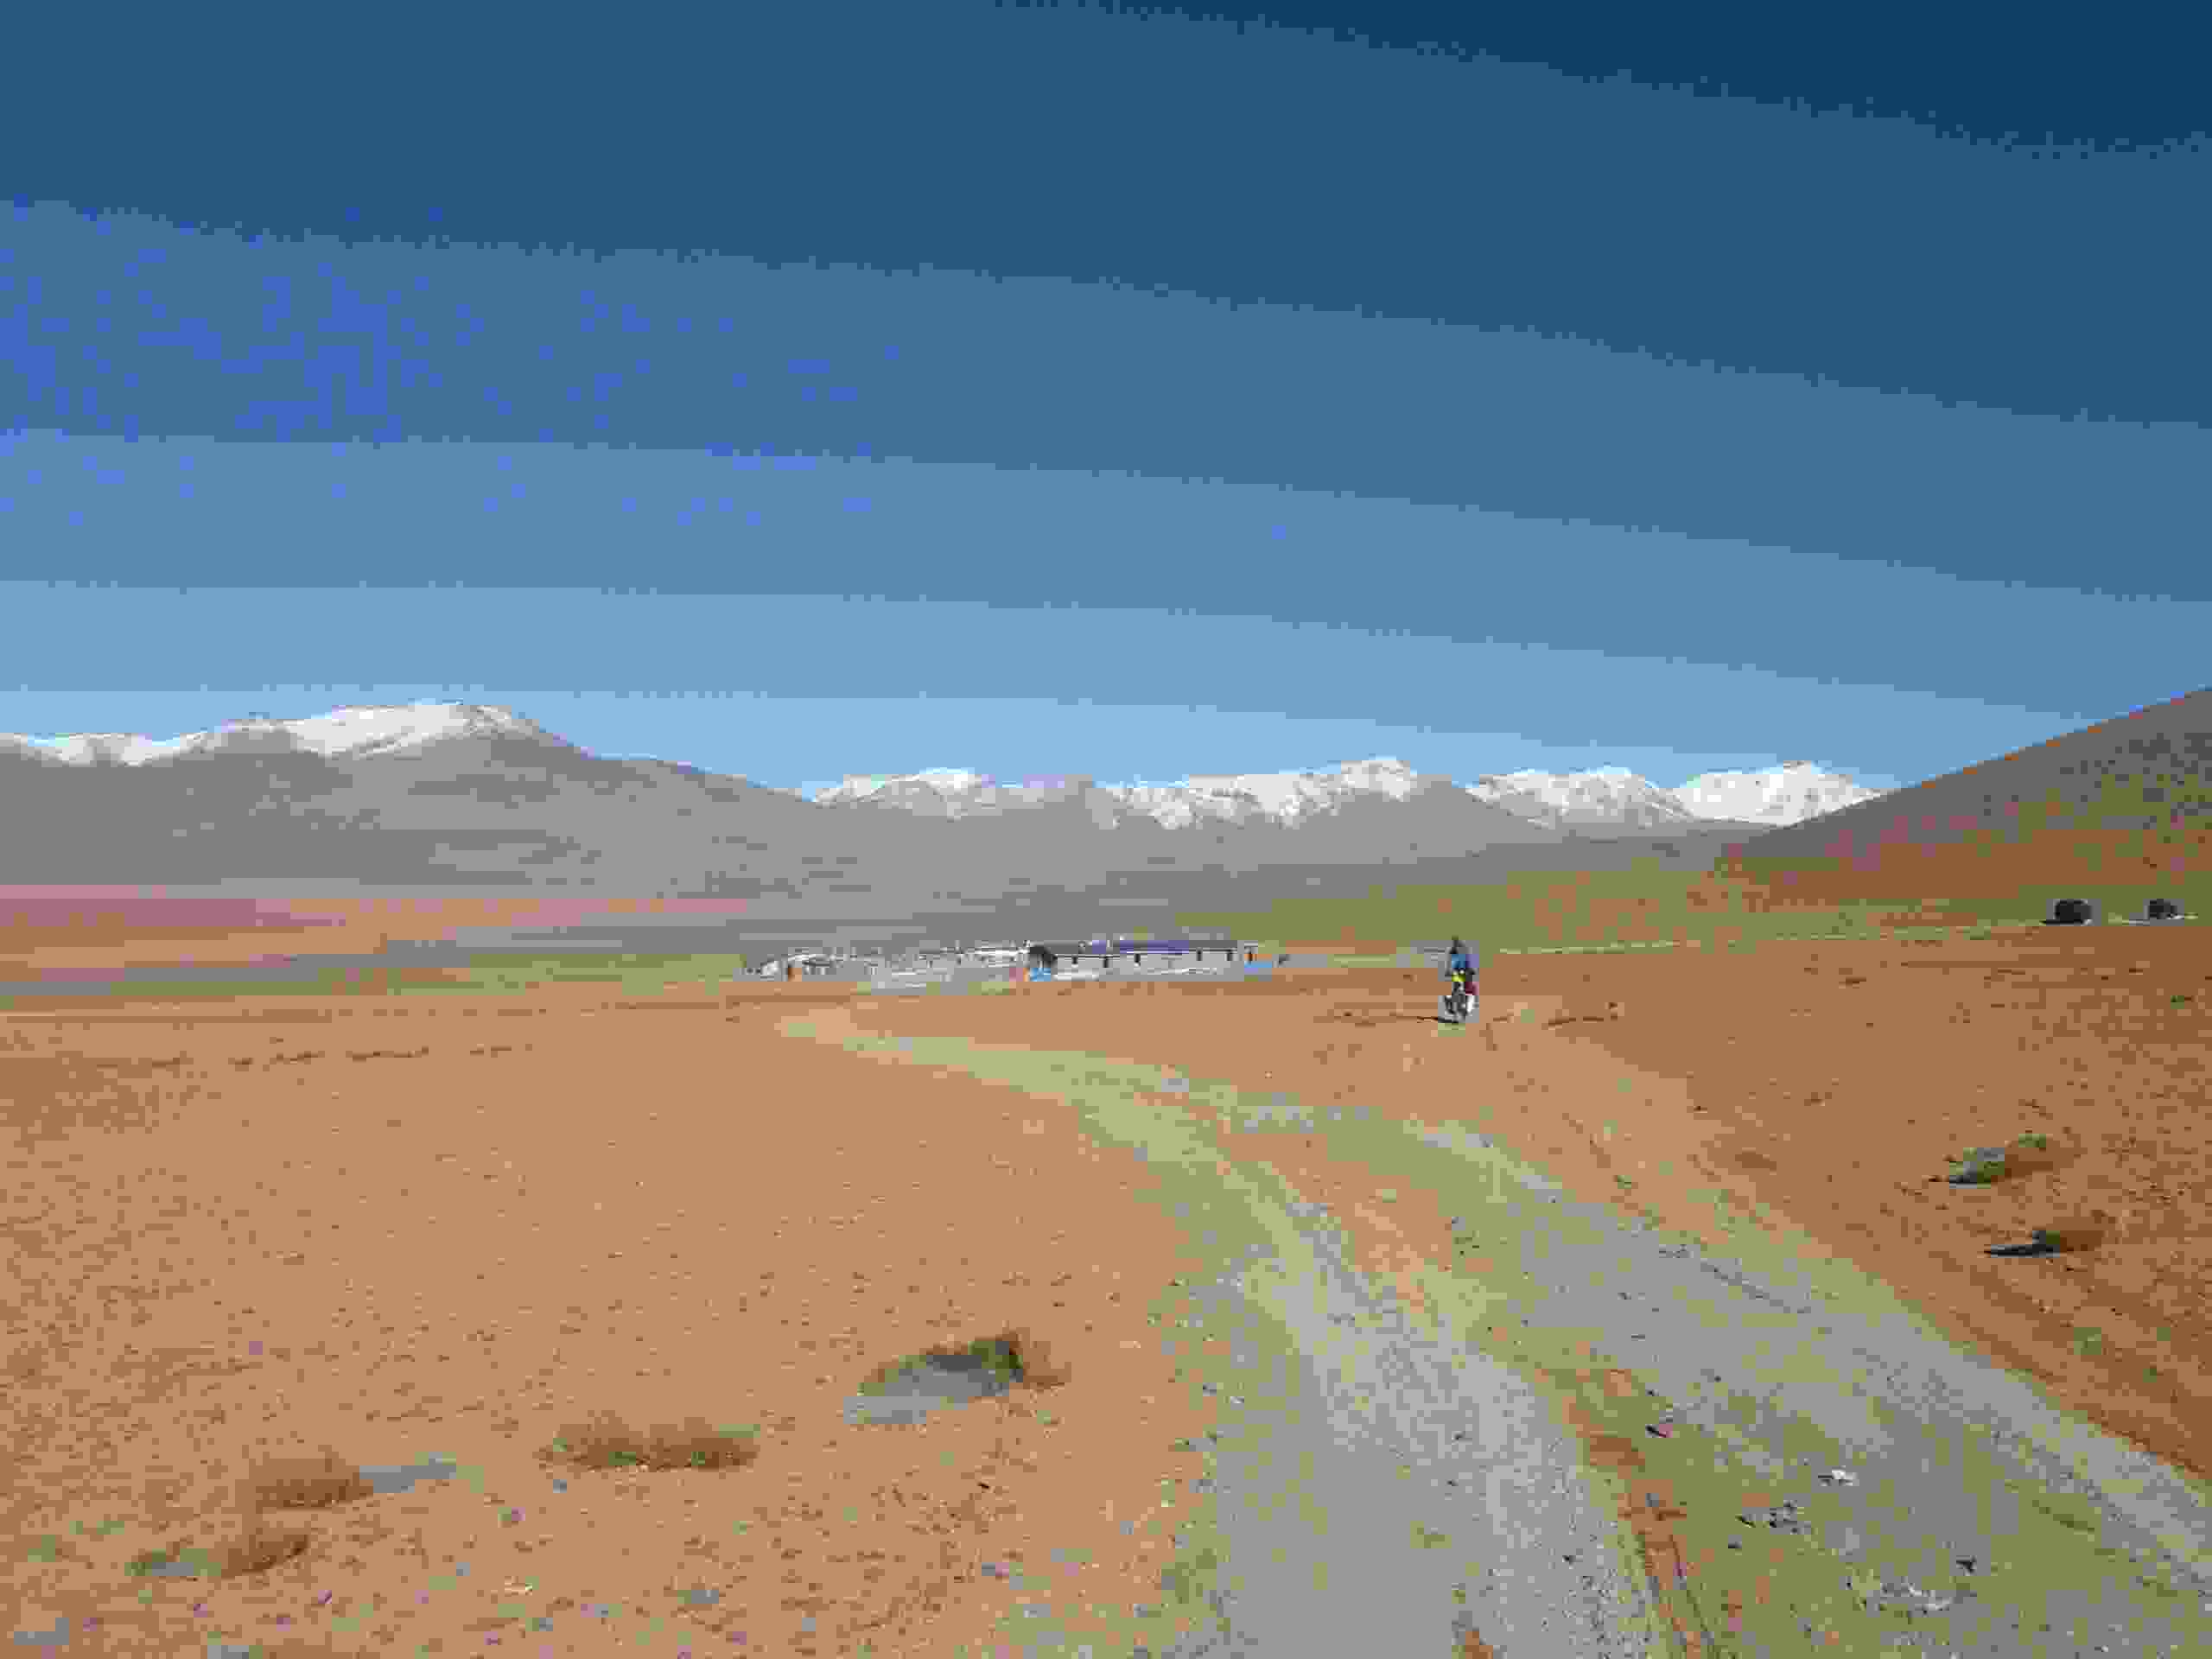
\includegraphics[width=\mywidth]{../wp-content/uploads/2015/04/wpid-wp-1427985164097.jpg} } 
 \newline
 \newline
\centerline{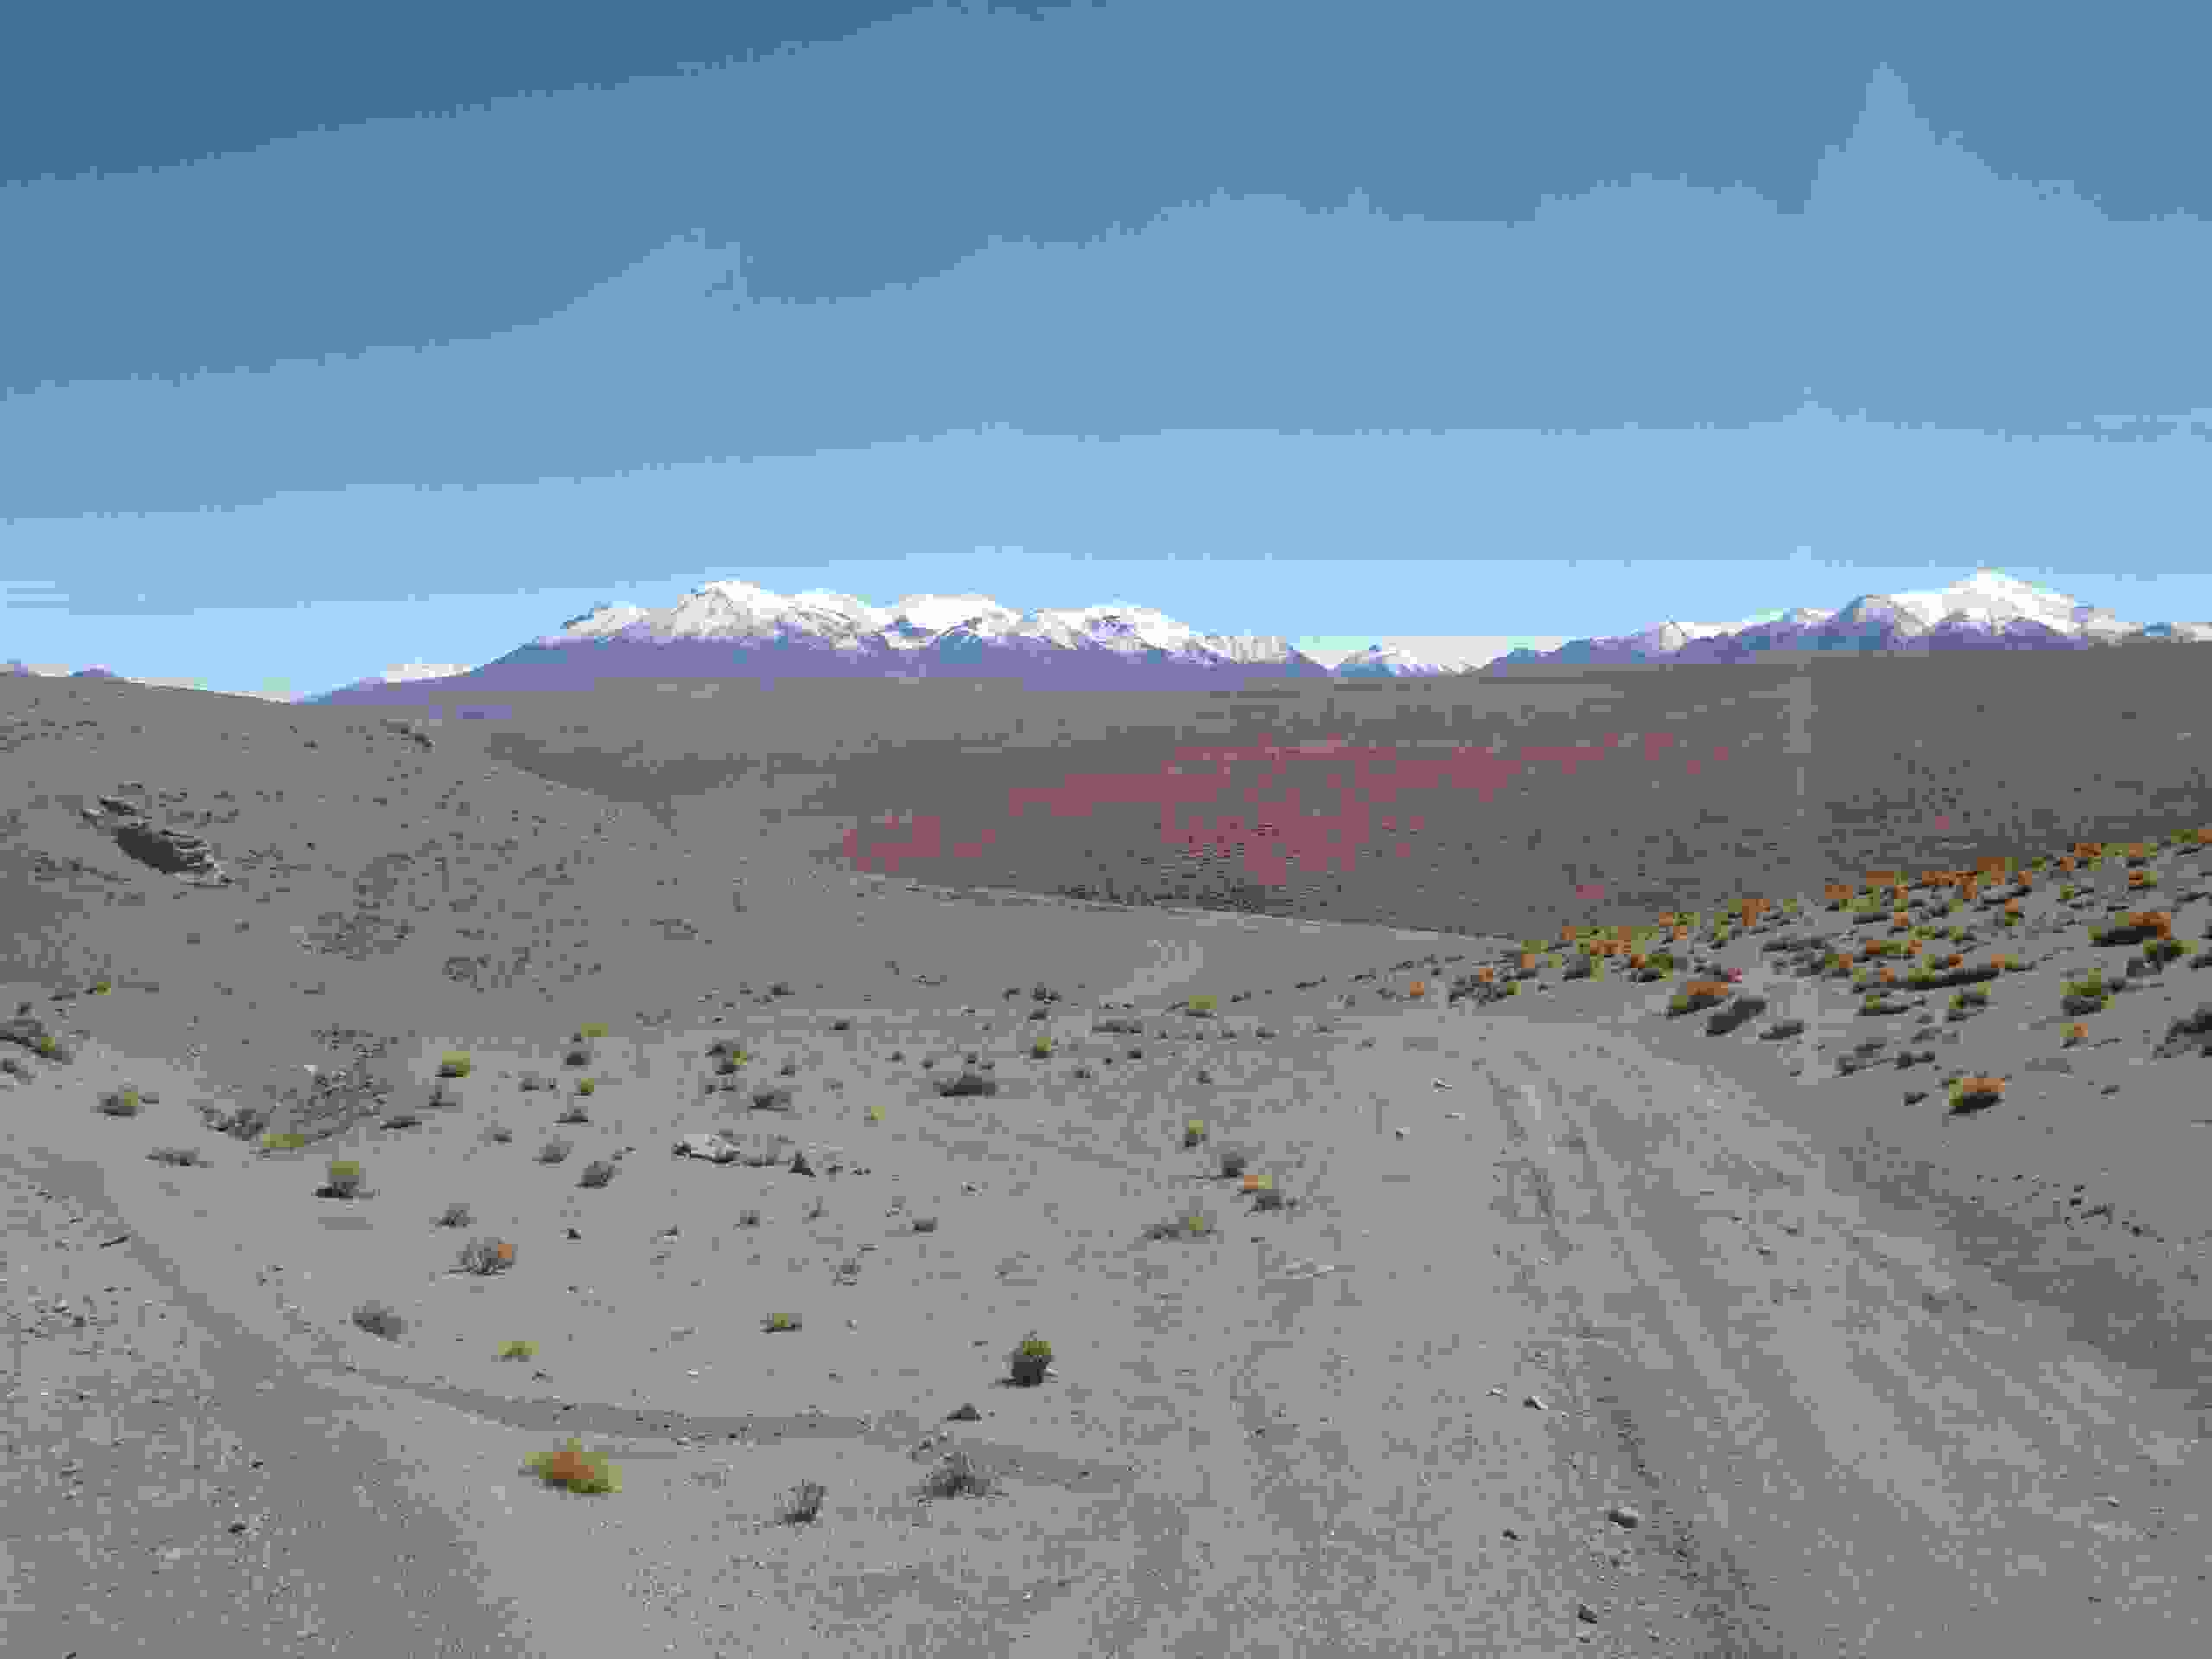
\includegraphics[width=\mywidth]{../wp-content/uploads/2015/04/wpid-wp-1427985190000.jpg} } 
 \newline
 Puis c'est la descente et on arrive sur une succession de lacs magnifiques. \newline
 \newline
\centerline{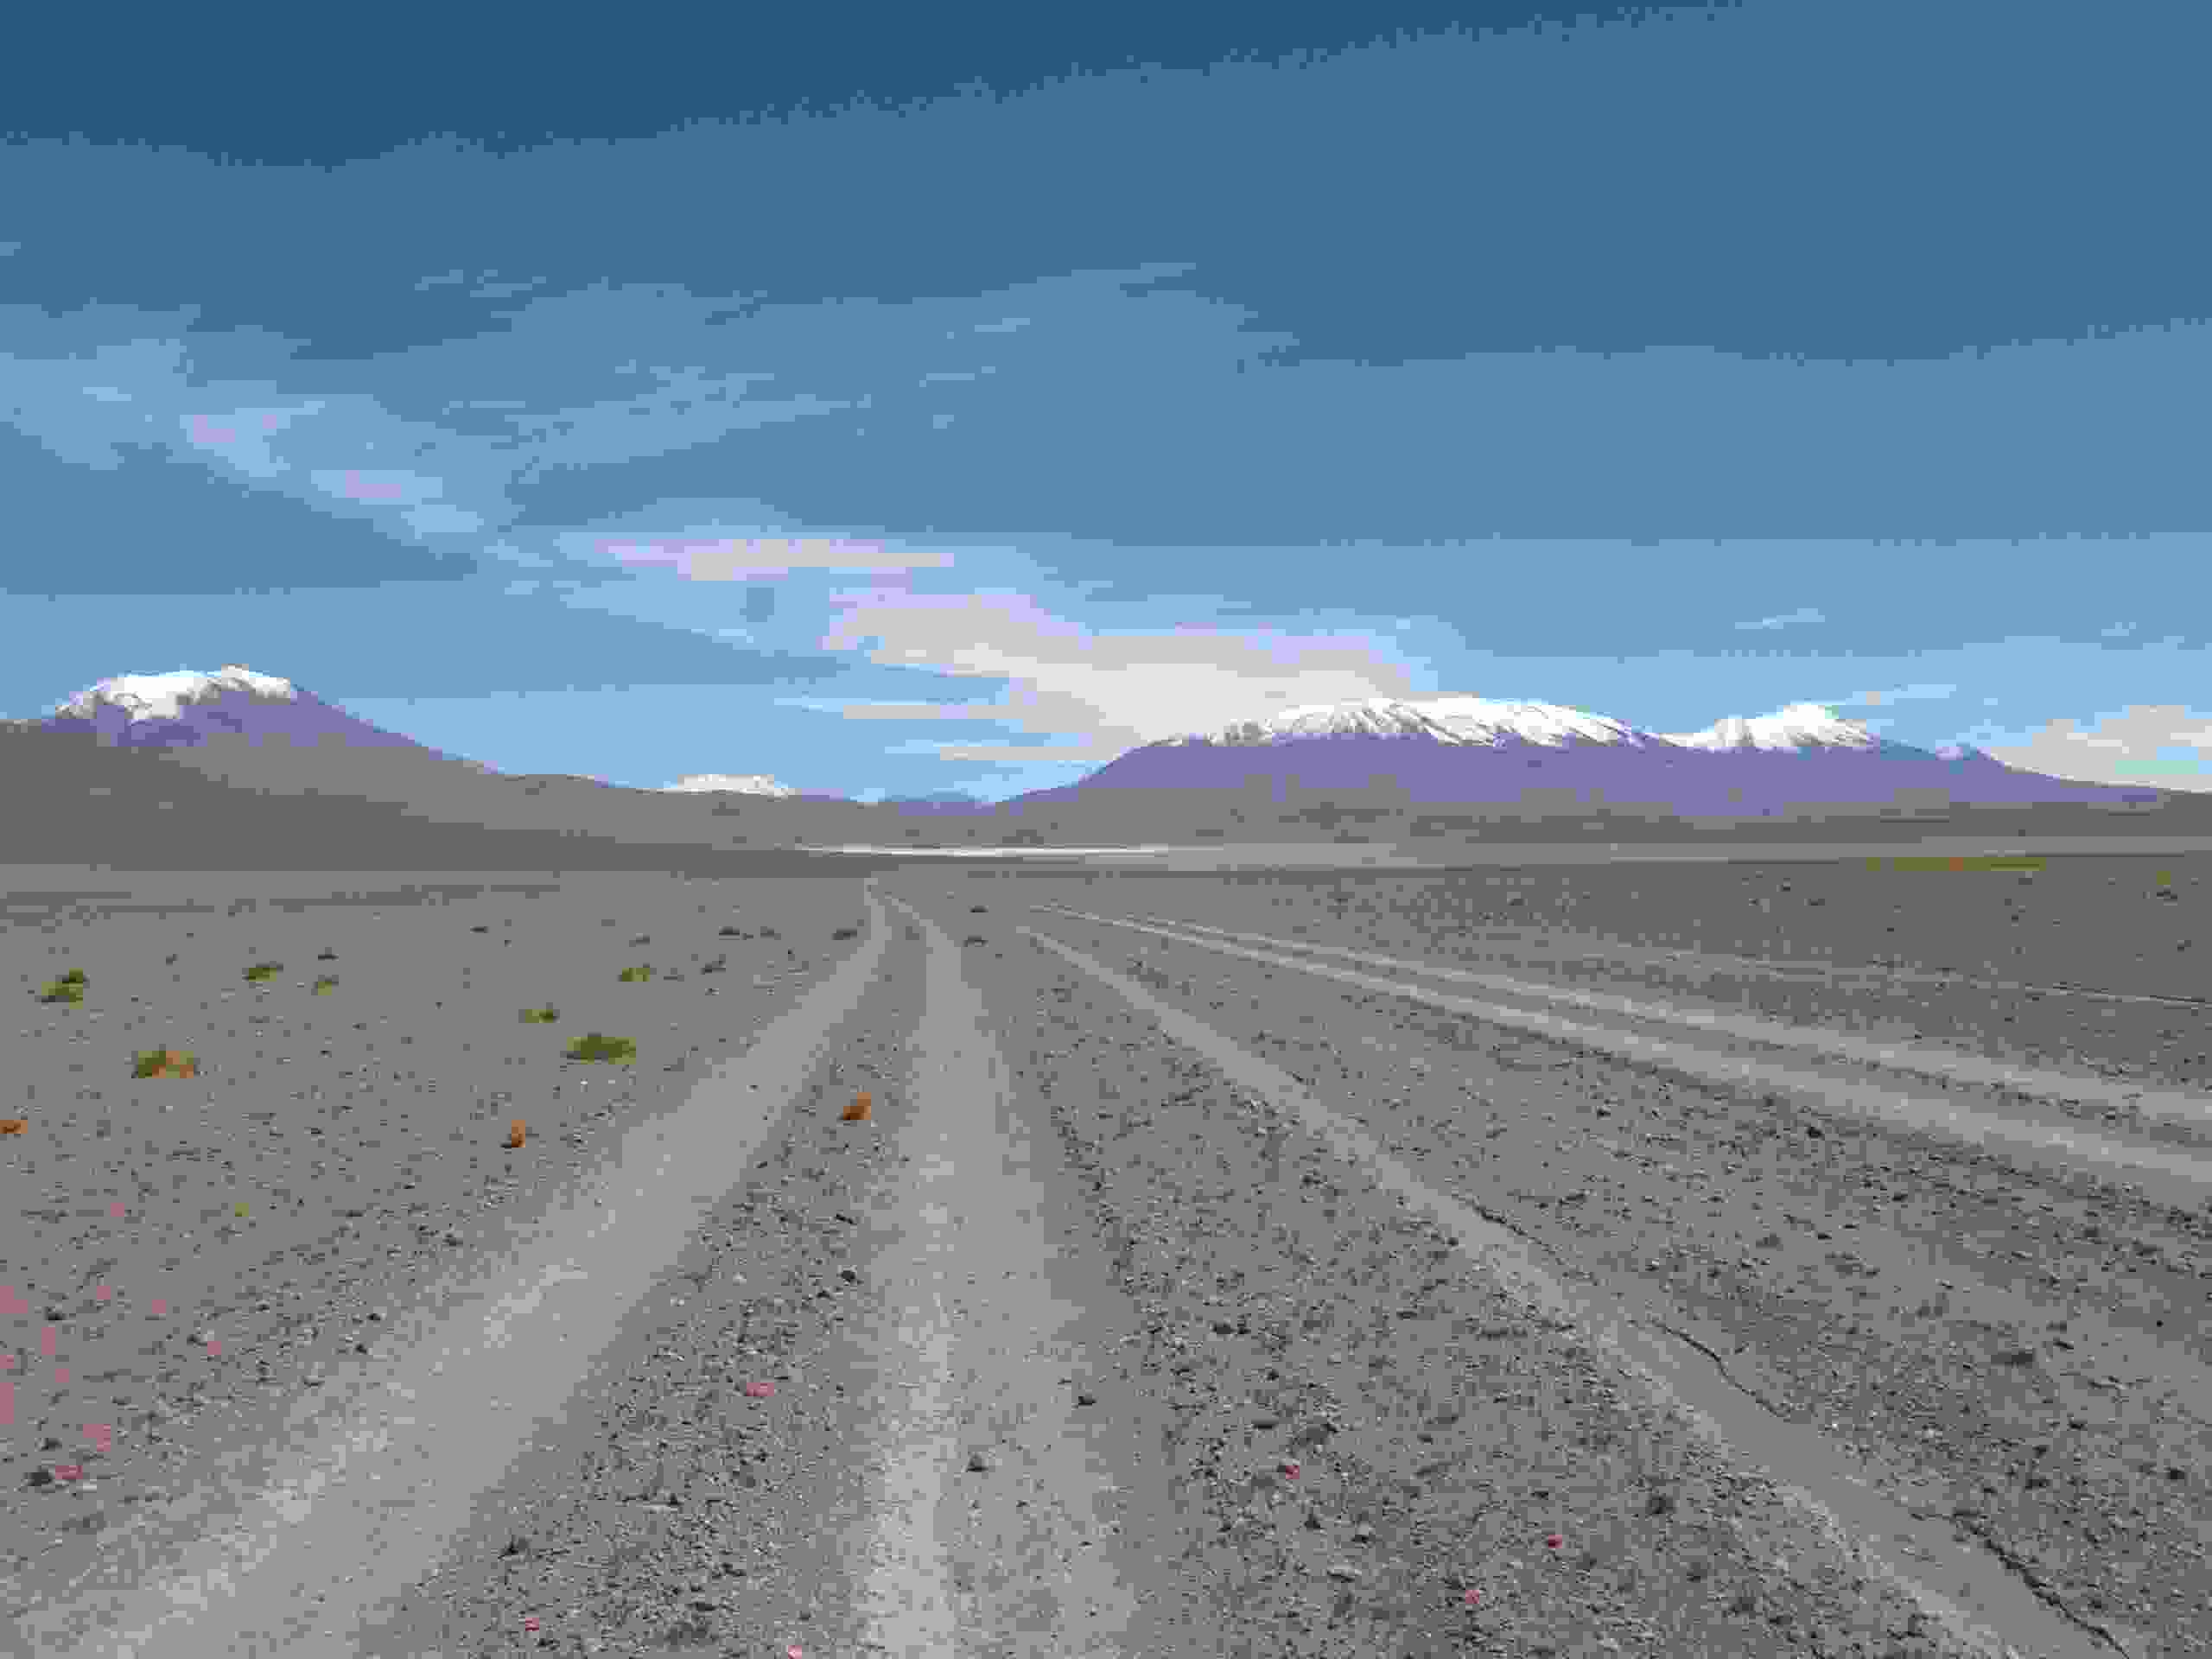
\includegraphics[width=\mywidth]{../wp-content/uploads/2015/04/wpid-wp-1427985235958.jpg} } 
 \newline
 \newline
\centerline{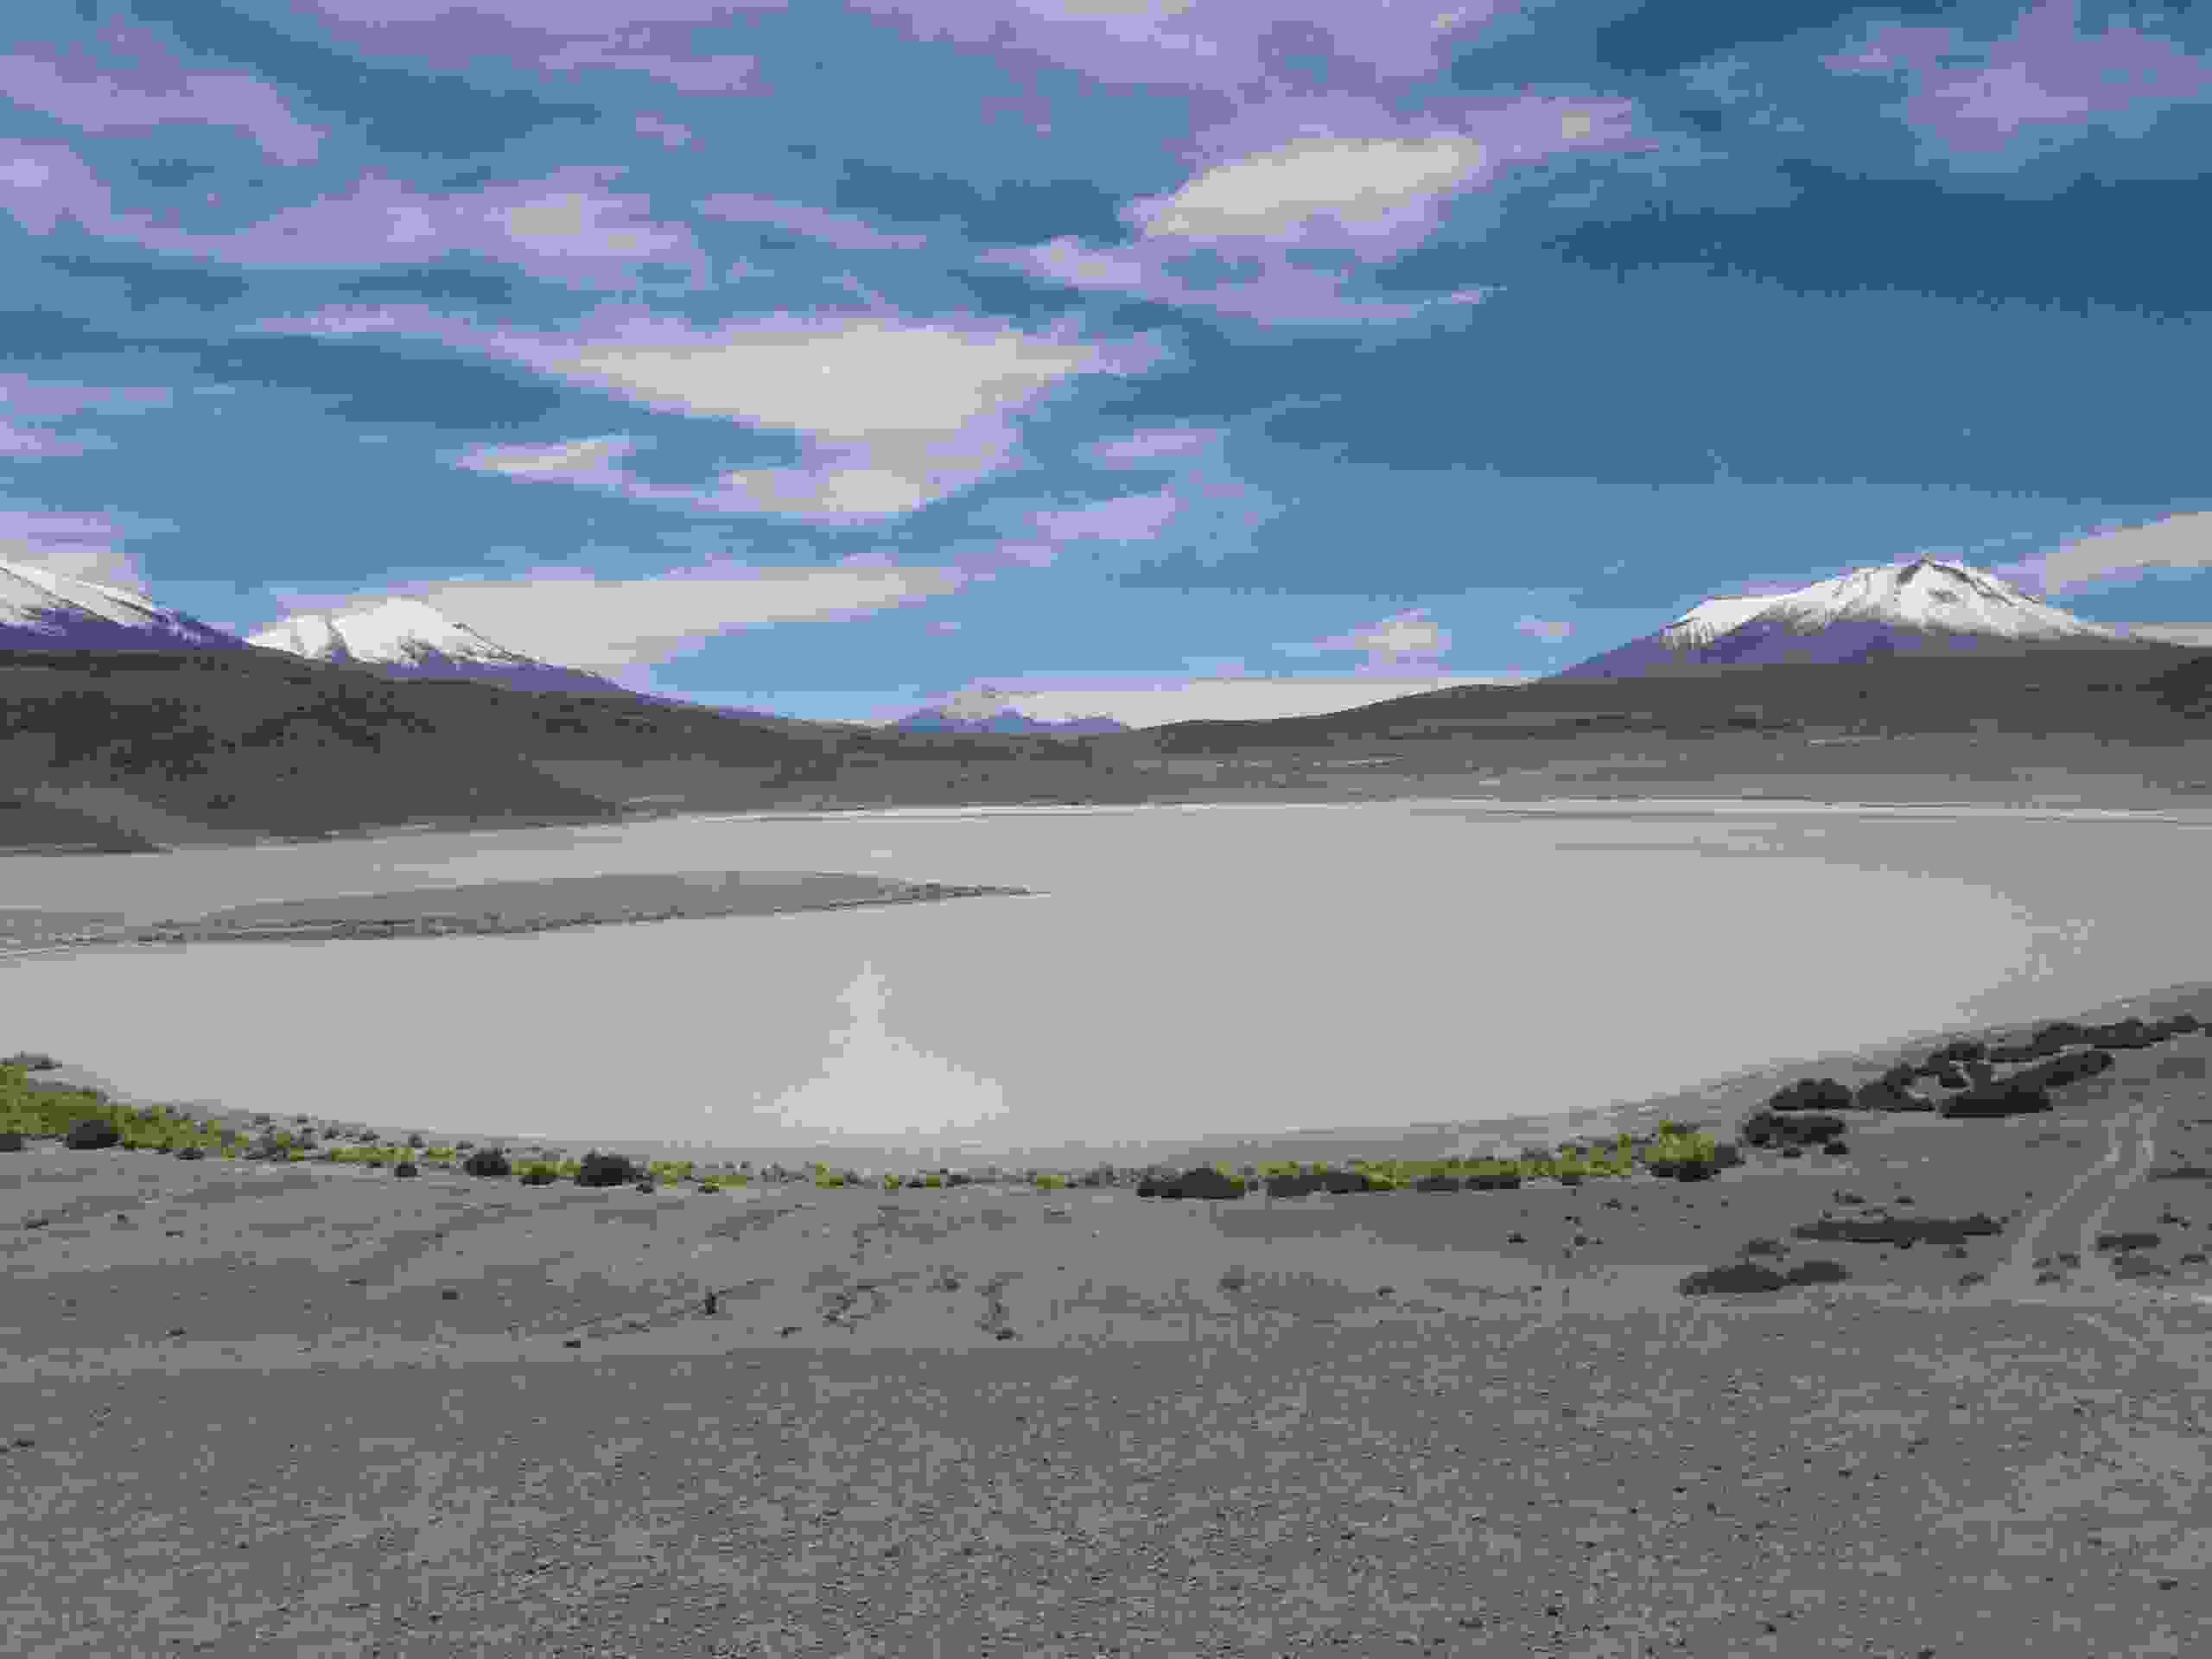
\includegraphics[width=\mywidth]{../wp-content/uploads/2015/04/wpid-wp-1427985282277.jpg} } 
 \newline
 \newline
\centerline{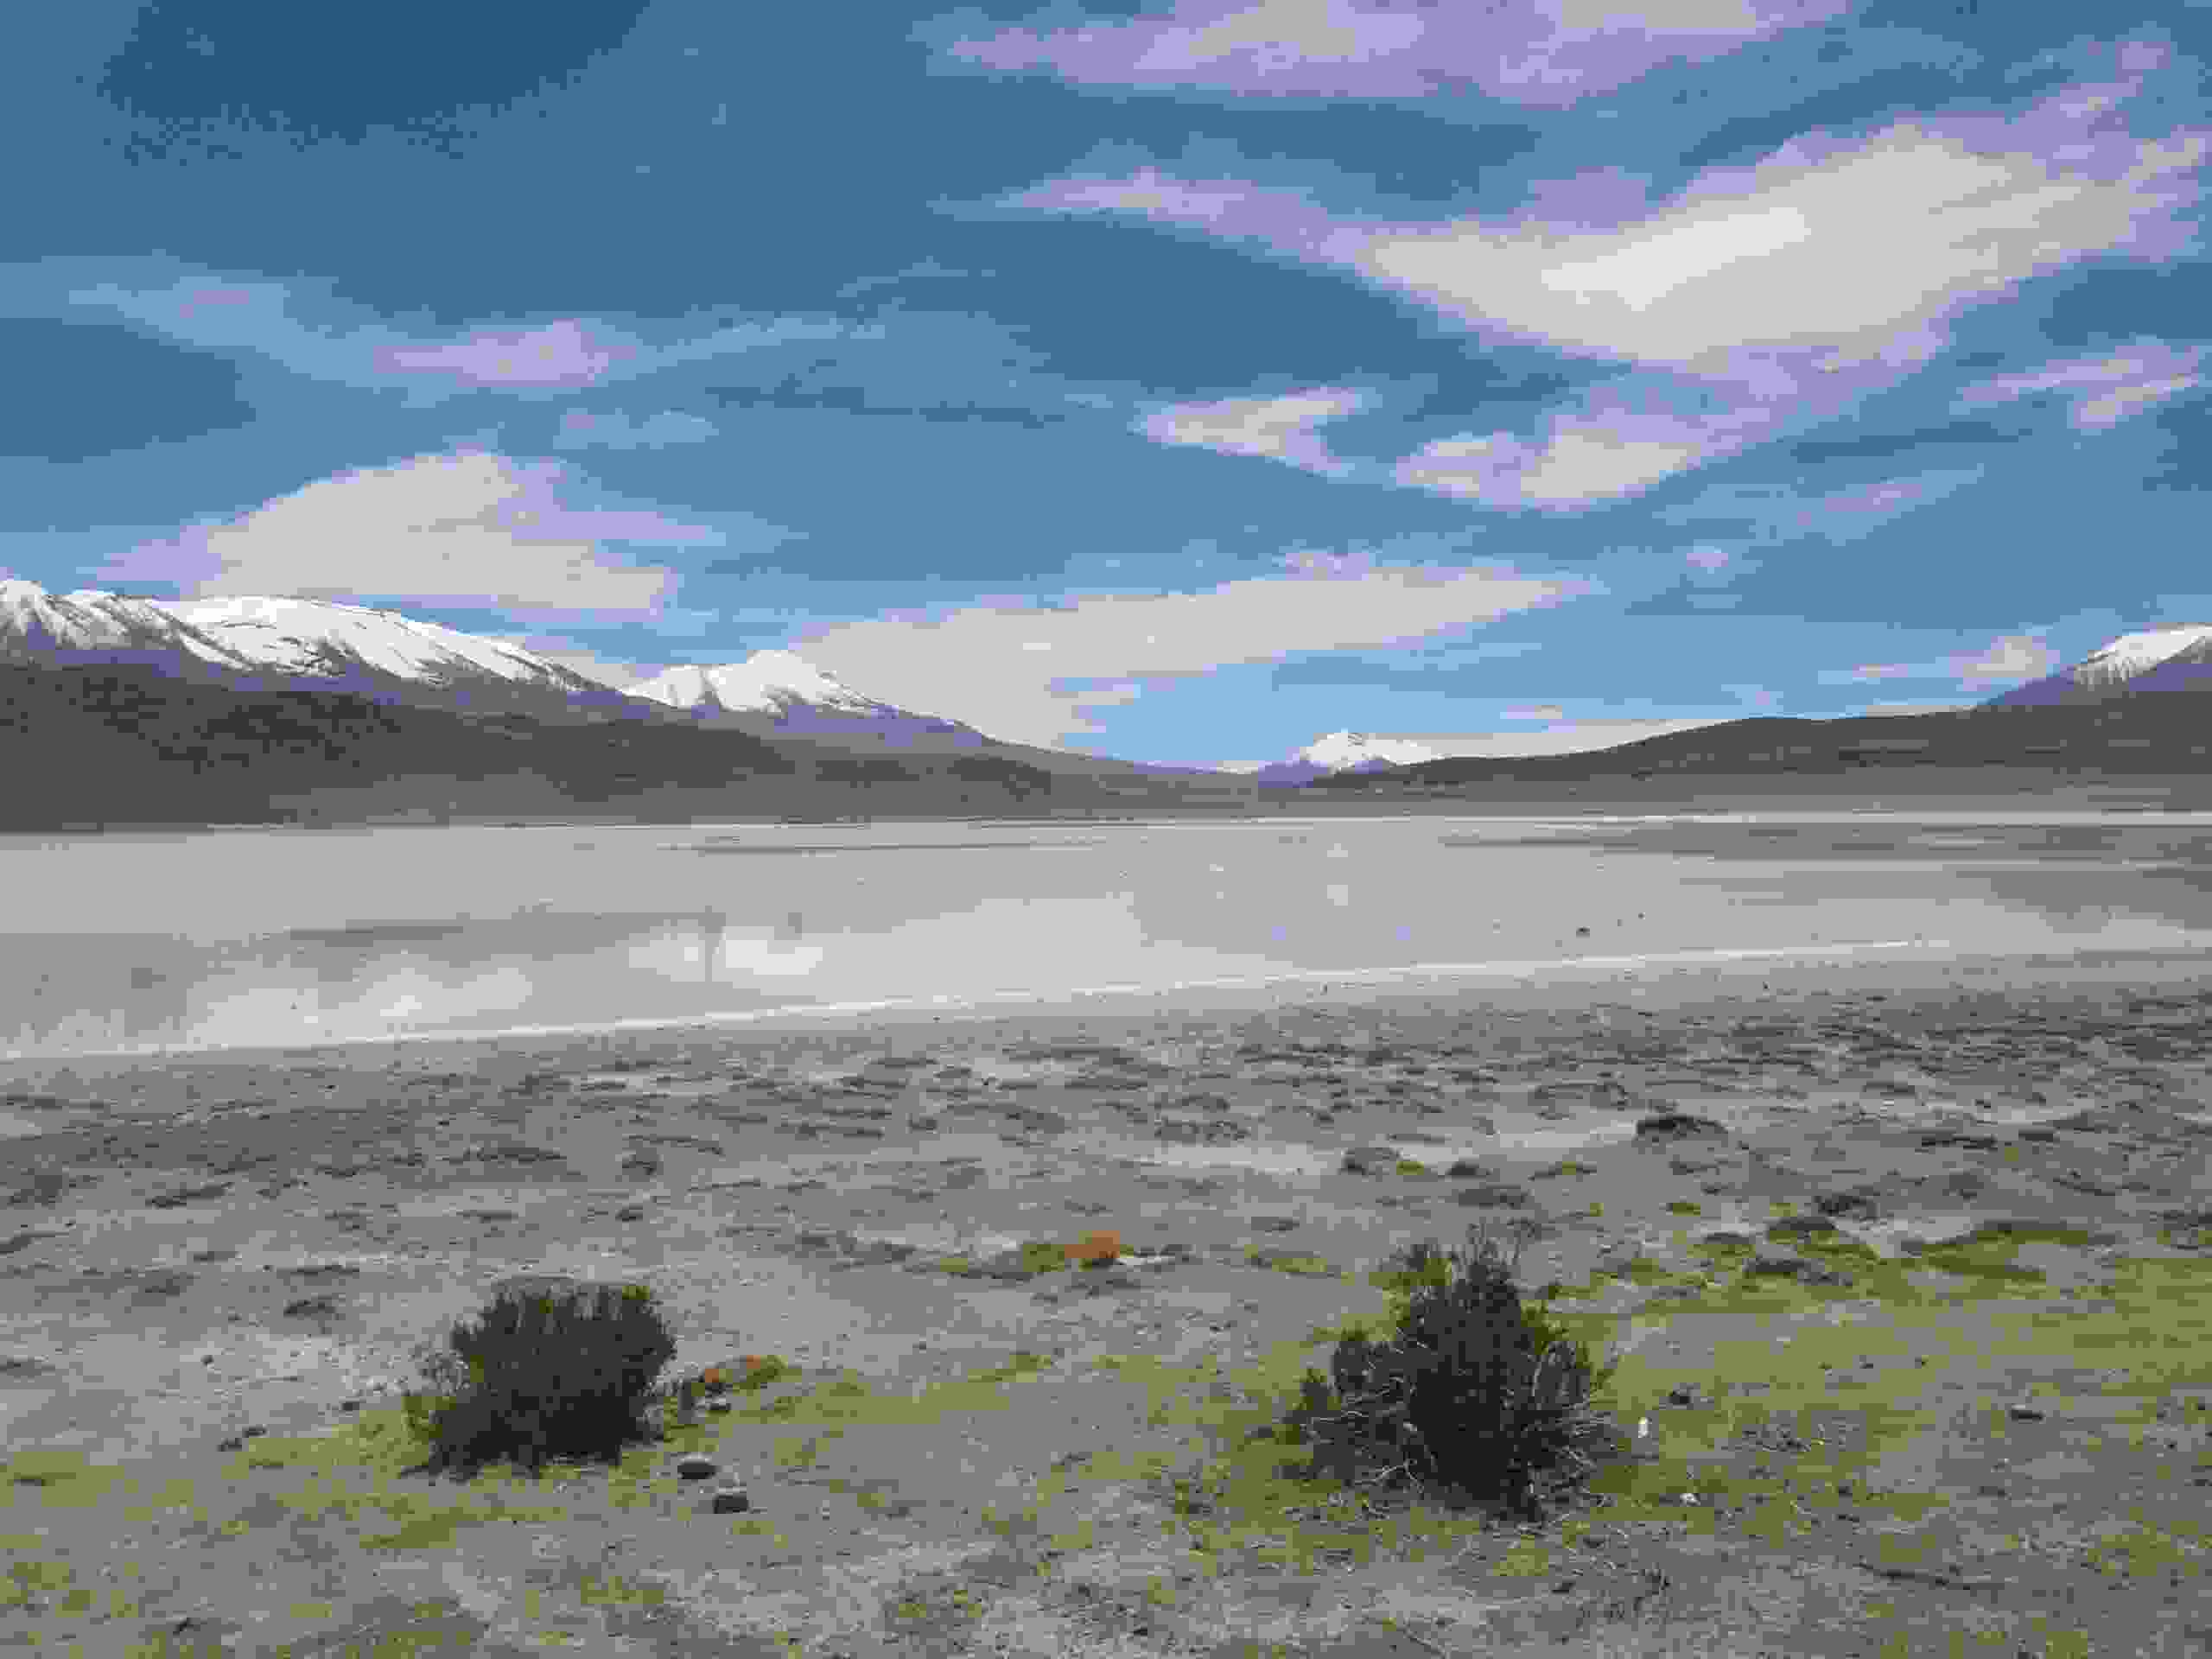
\includegraphics[width=\mywidth]{../wp-content/uploads/2015/04/wpid-wp-1427985322344.jpg} } 
 \newline
 \newline
\centerline{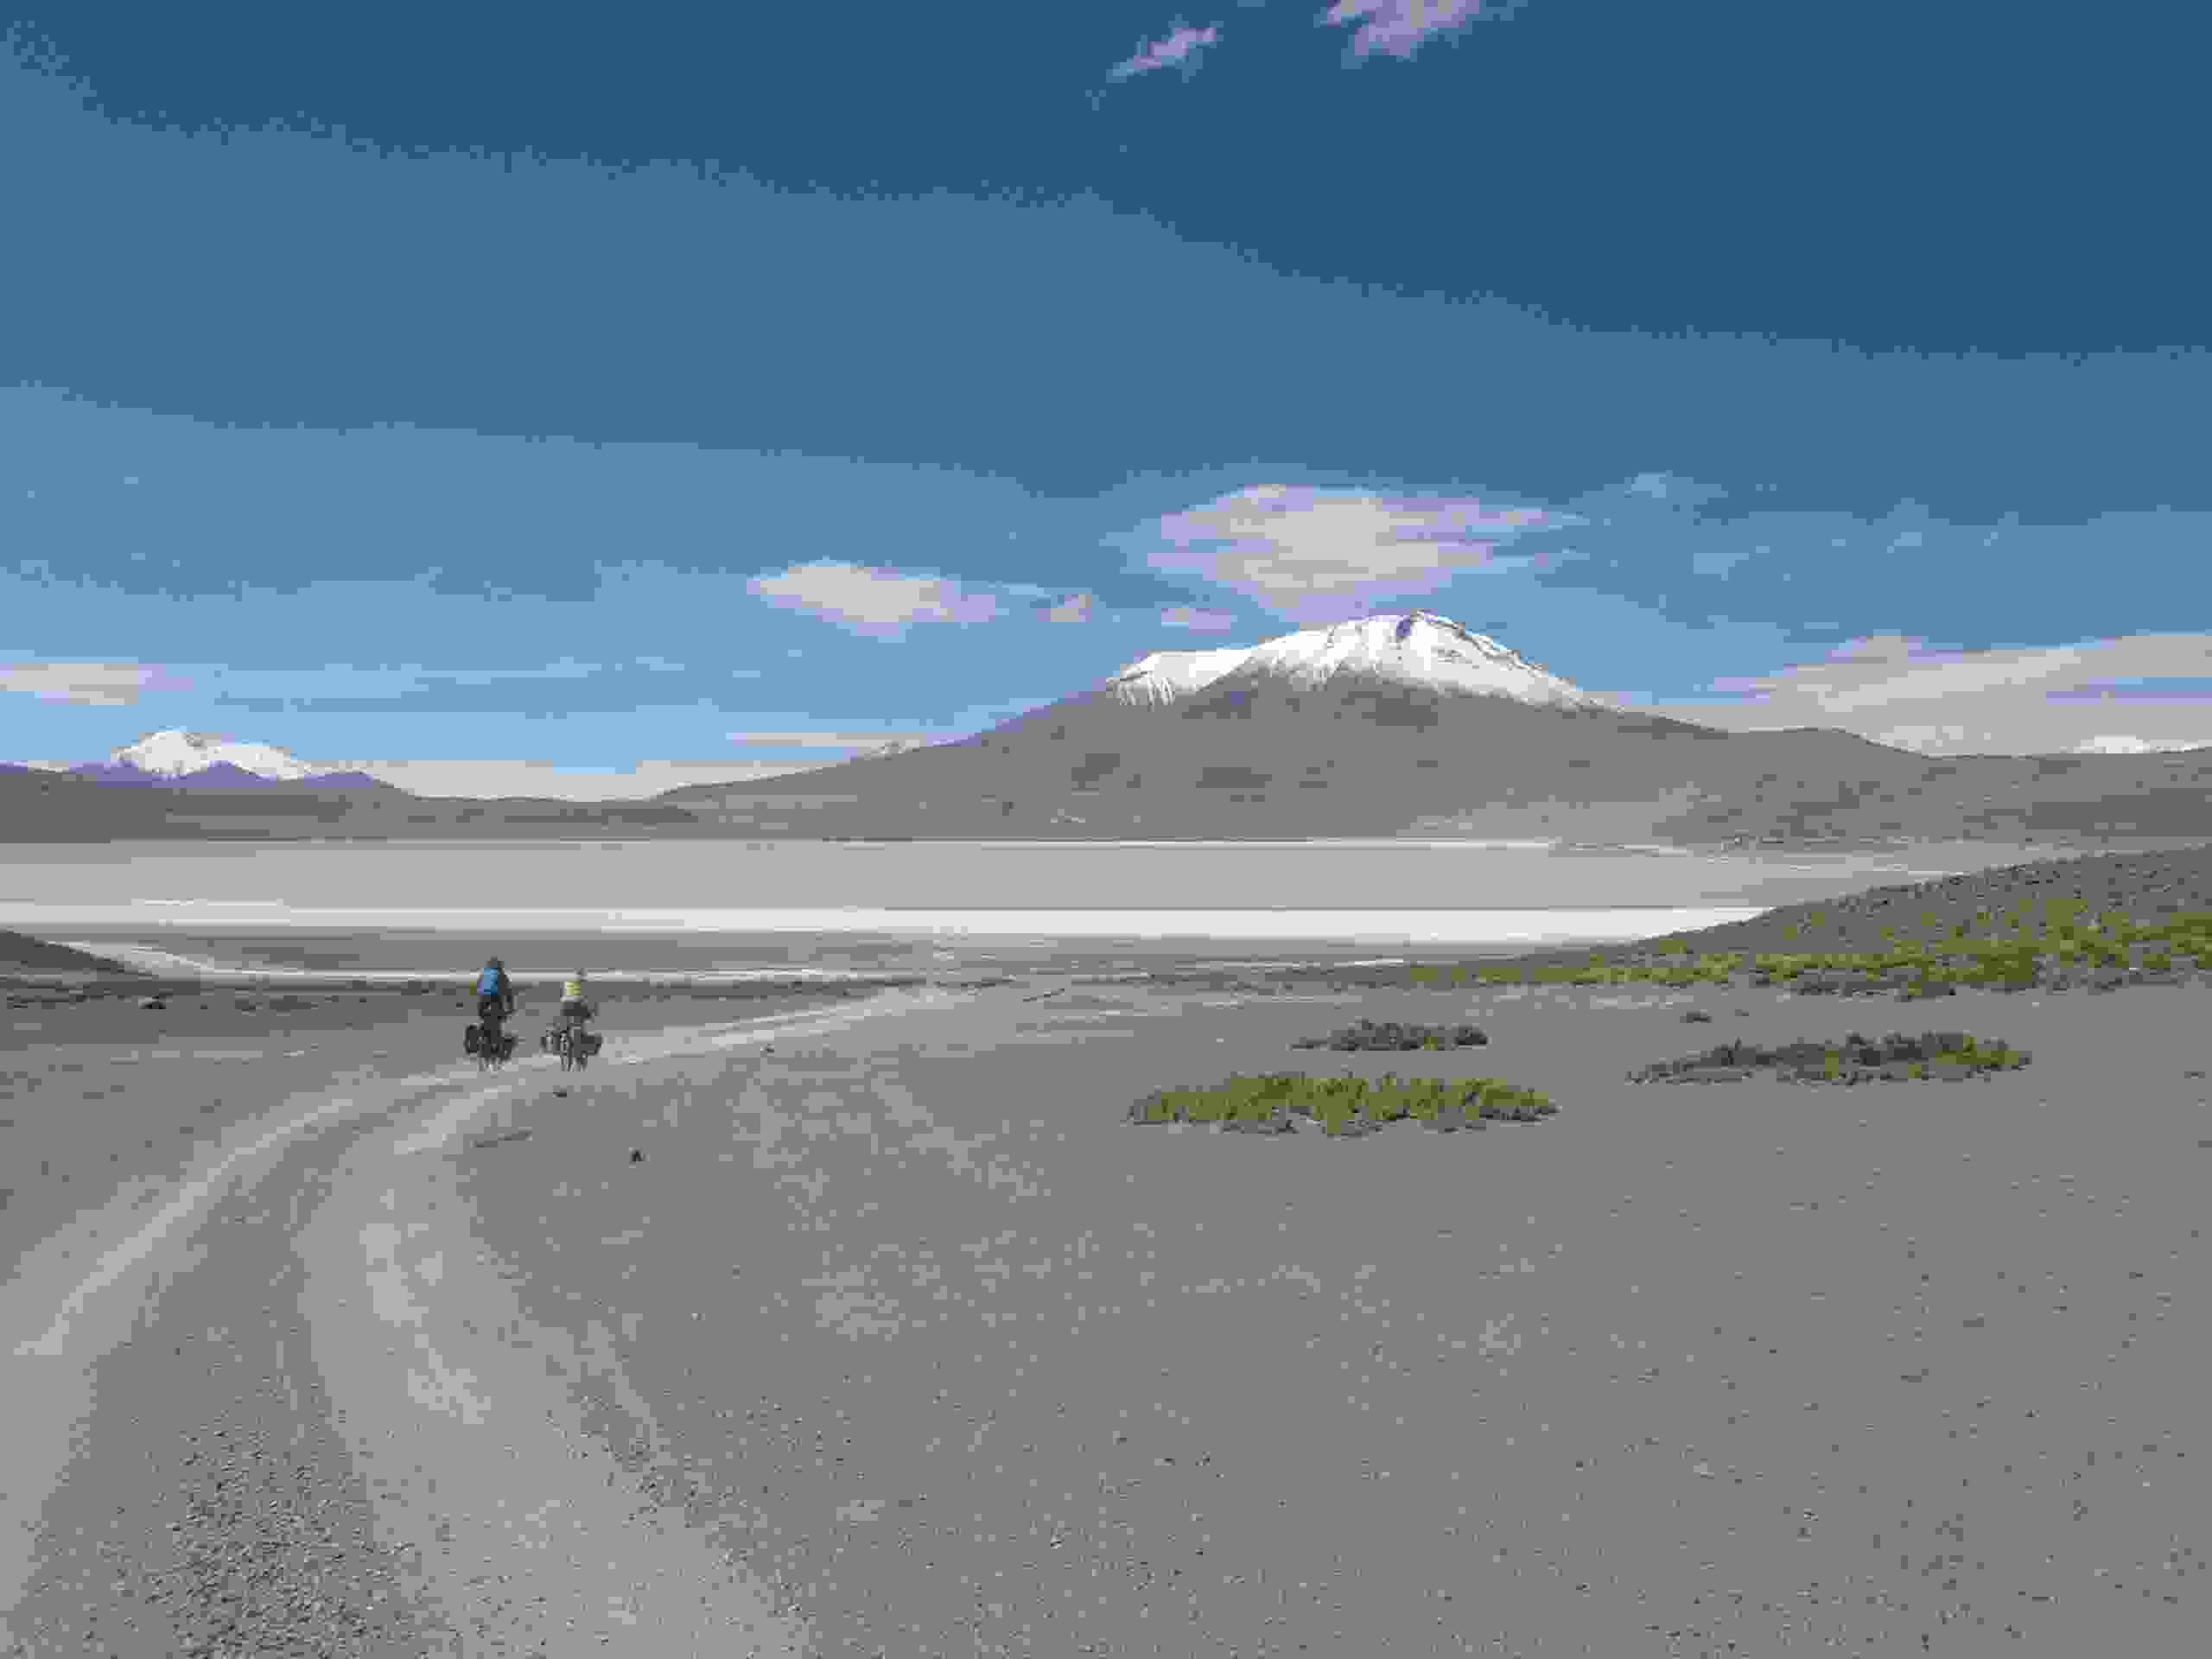
\includegraphics[width=\mywidth]{../wp-content/uploads/2015/04/wpid-wp-1427985384246.jpg} } 
 \newline
 Pour terminer à la Laguna Hedionda. \newline
 \newline
\centerline{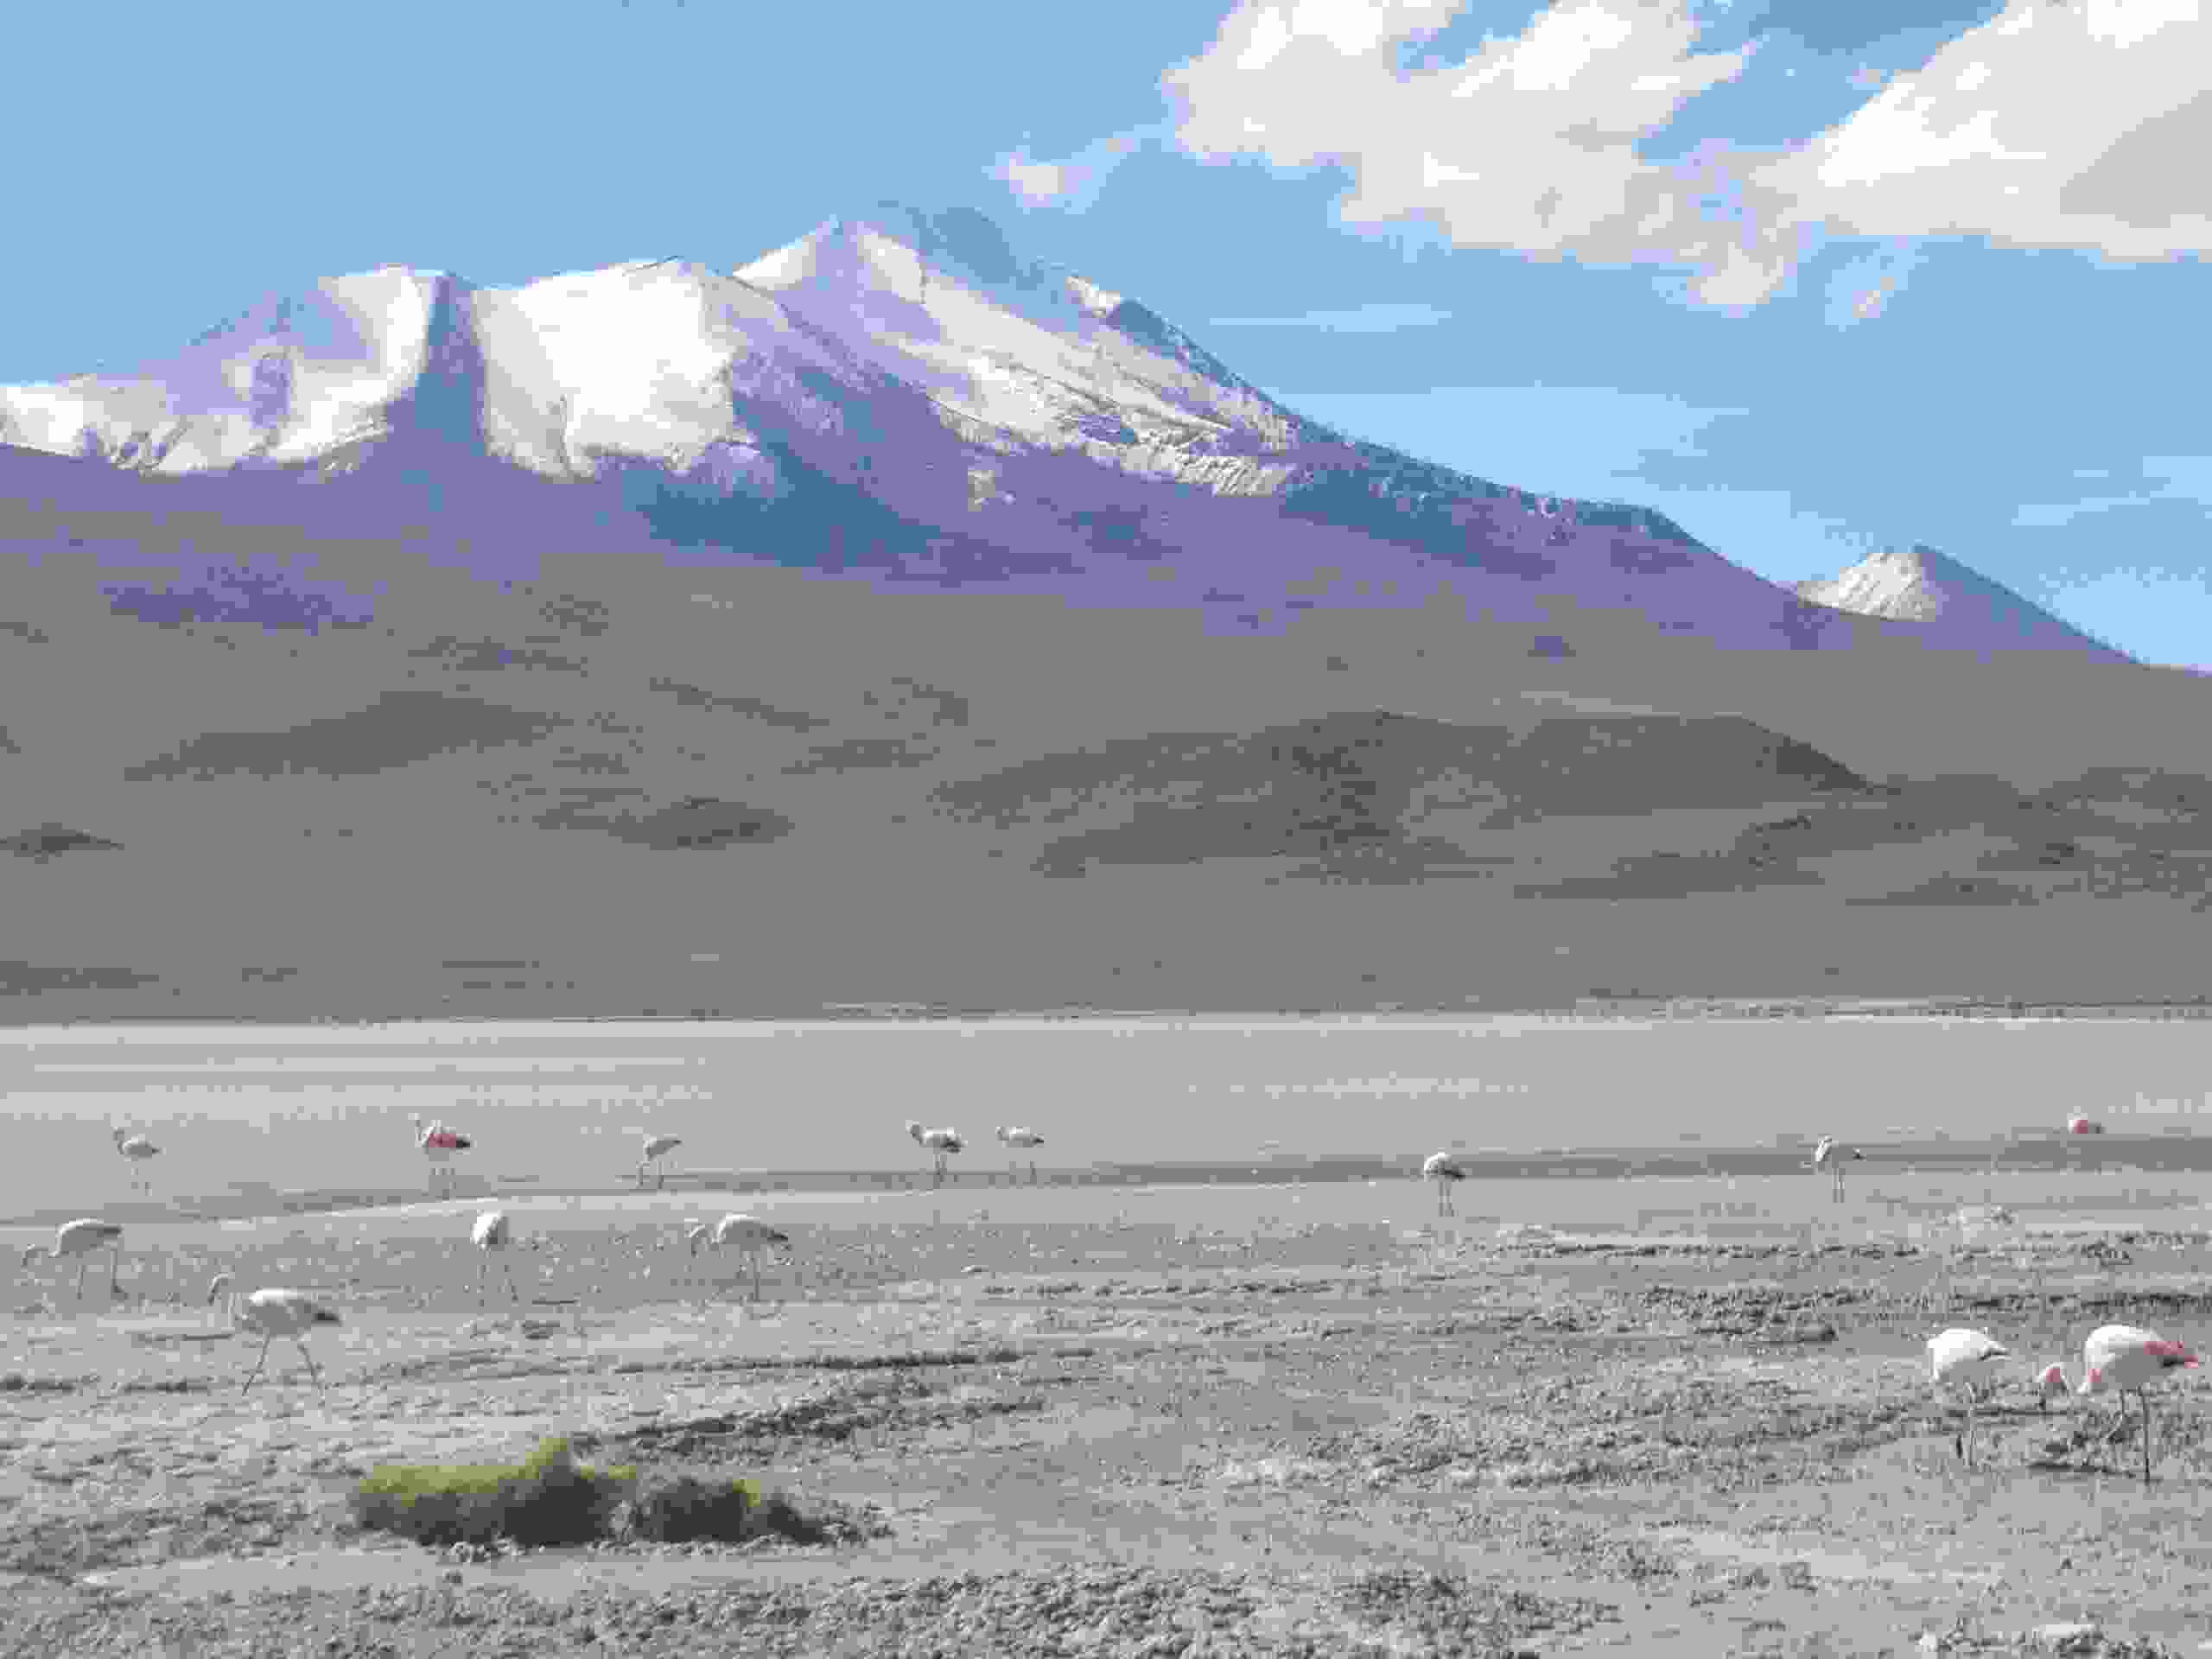
\includegraphics[width=\mywidth]{../wp-content/uploads/2015/04/wpid-wp-1427985428387.jpg} } 
 \newline
 \newline
\centerline{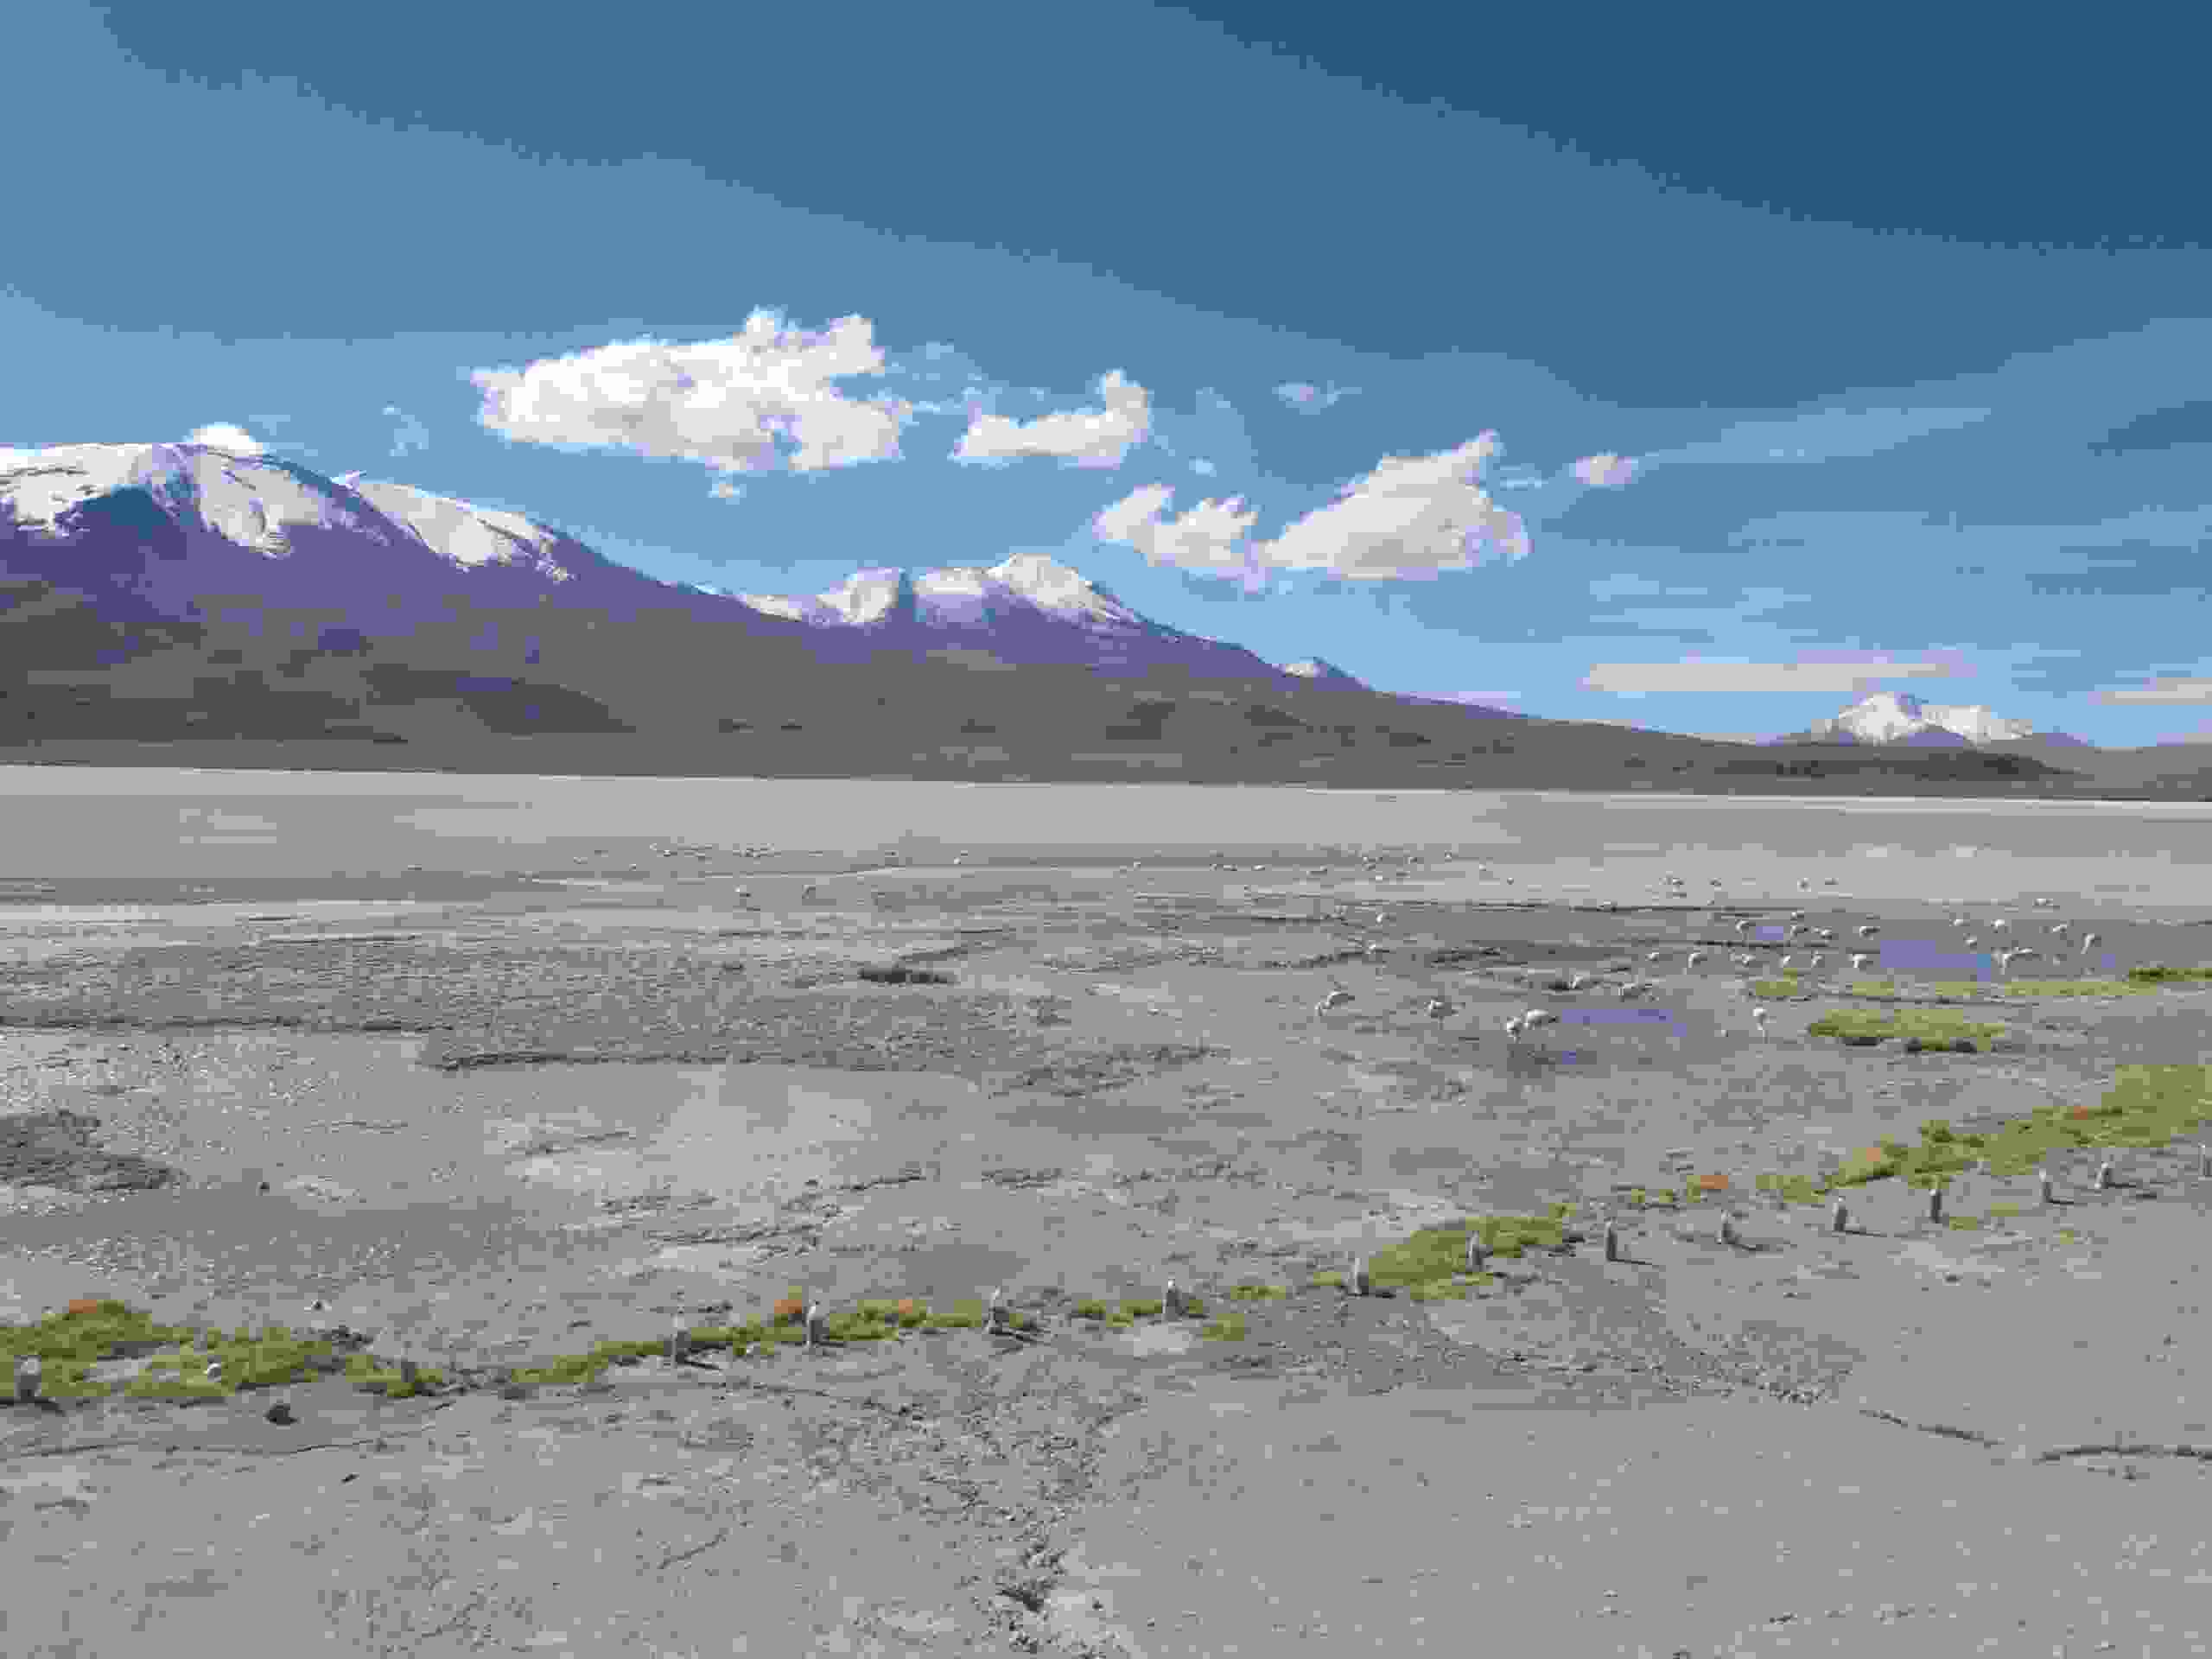
\includegraphics[width=\mywidth]{../wp-content/uploads/2015/04/wpid-wp-1427985446476.jpg} } 
 \newline
 \newline
\centerline{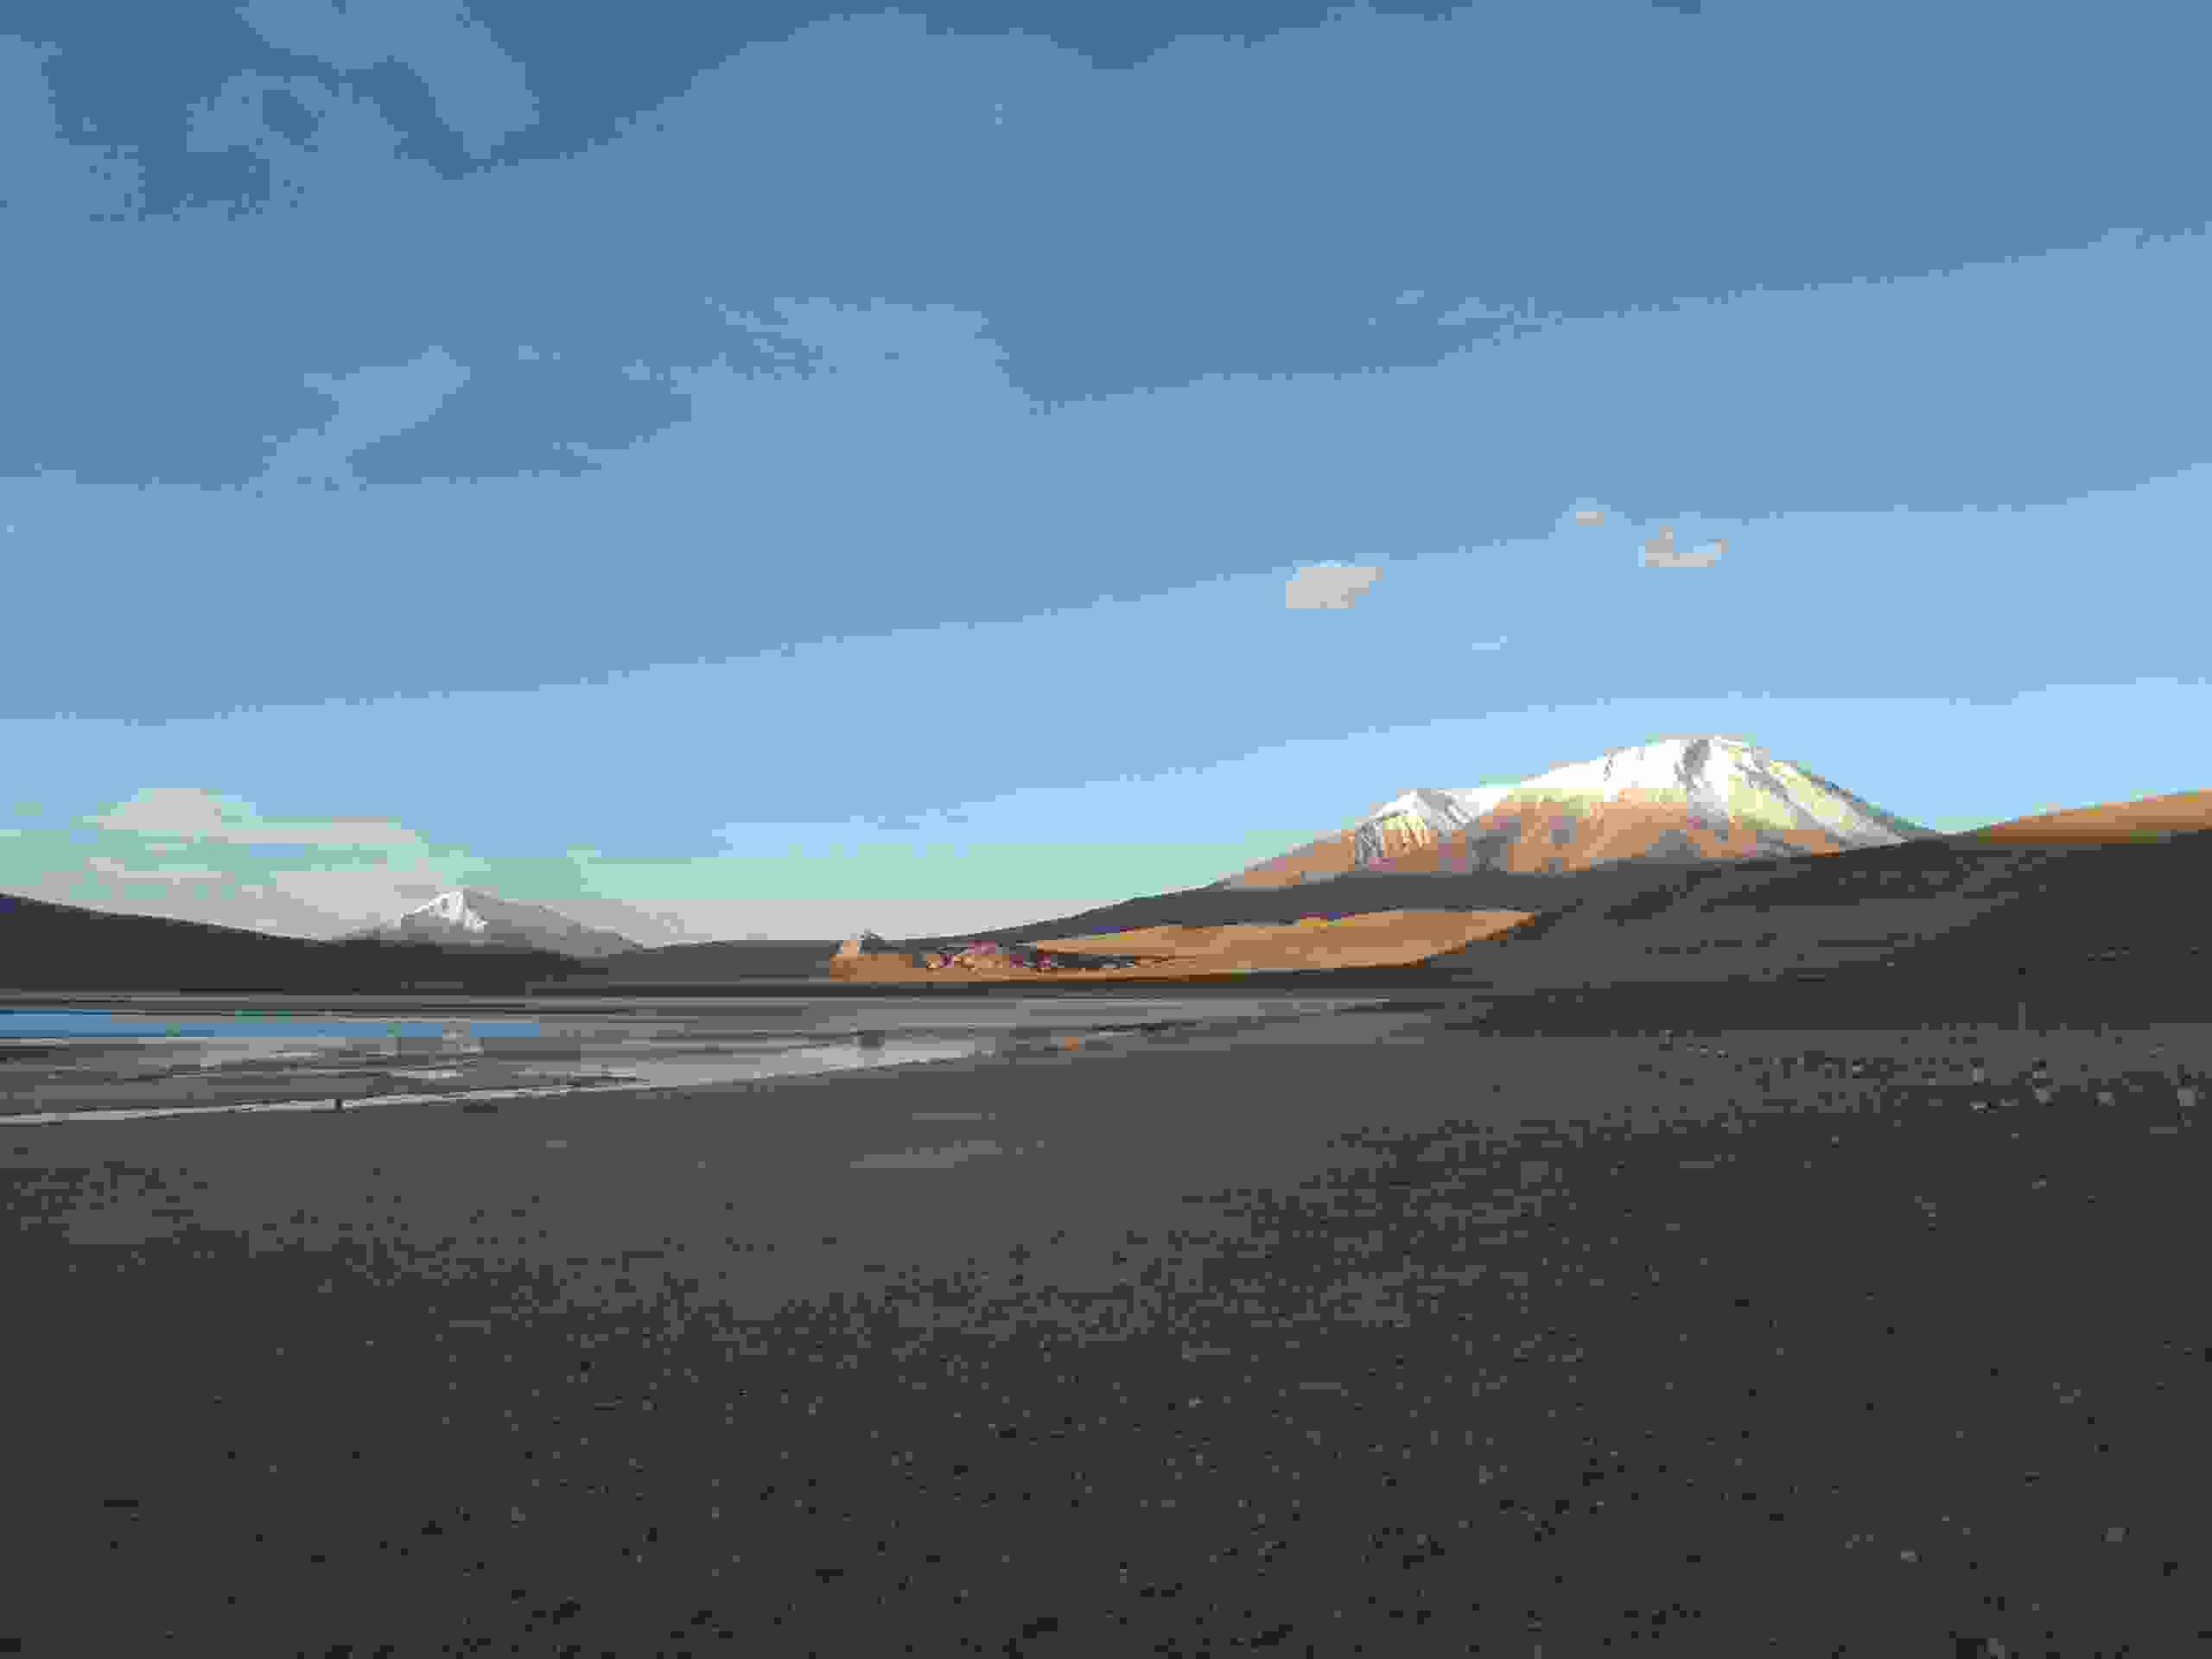
\includegraphics[width=\mywidth]{../wp-content/uploads/2015/04/wpid-wp-1427985493186.jpg} } 
 \newline
 \newline
\centerline{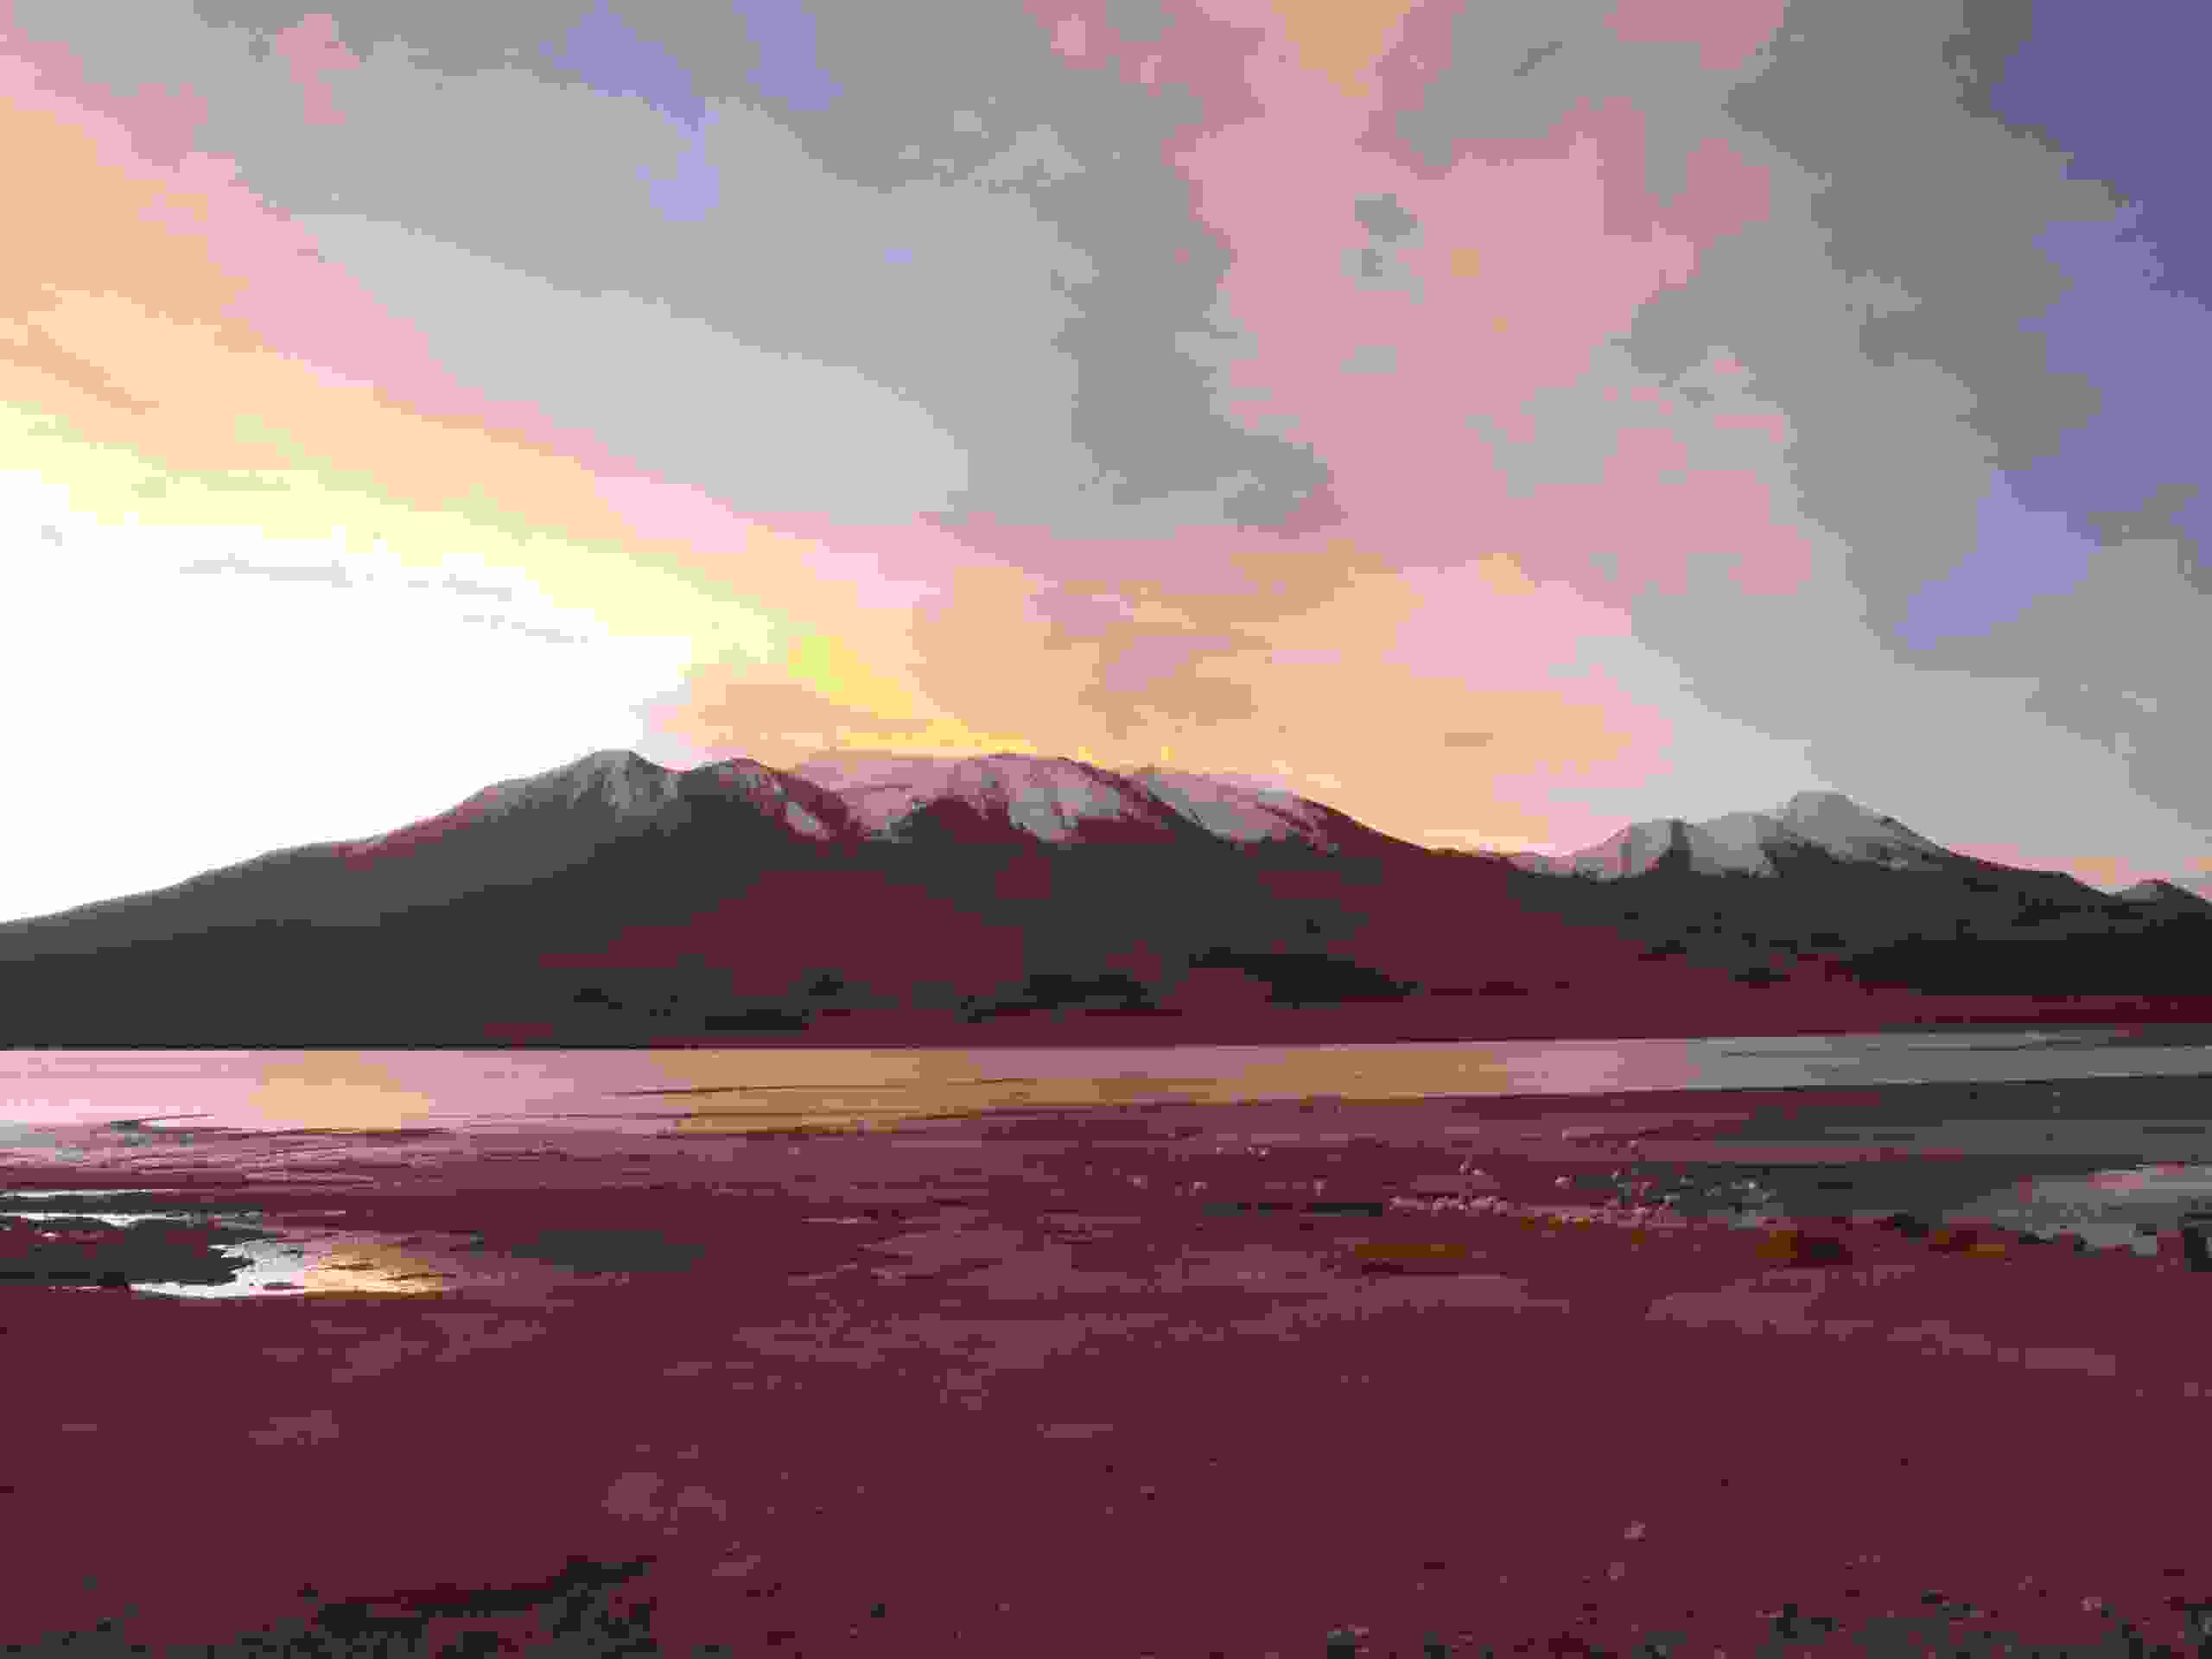
\includegraphics[width=\mywidth]{../wp-content/uploads/2015/04/wpid-wp-1427985509761.jpg} } 
 \newline
 8e jour : \newline
 Encore de la piste entre sable, cailloux et tôle ondulée : \newline
 \newline
\centerline{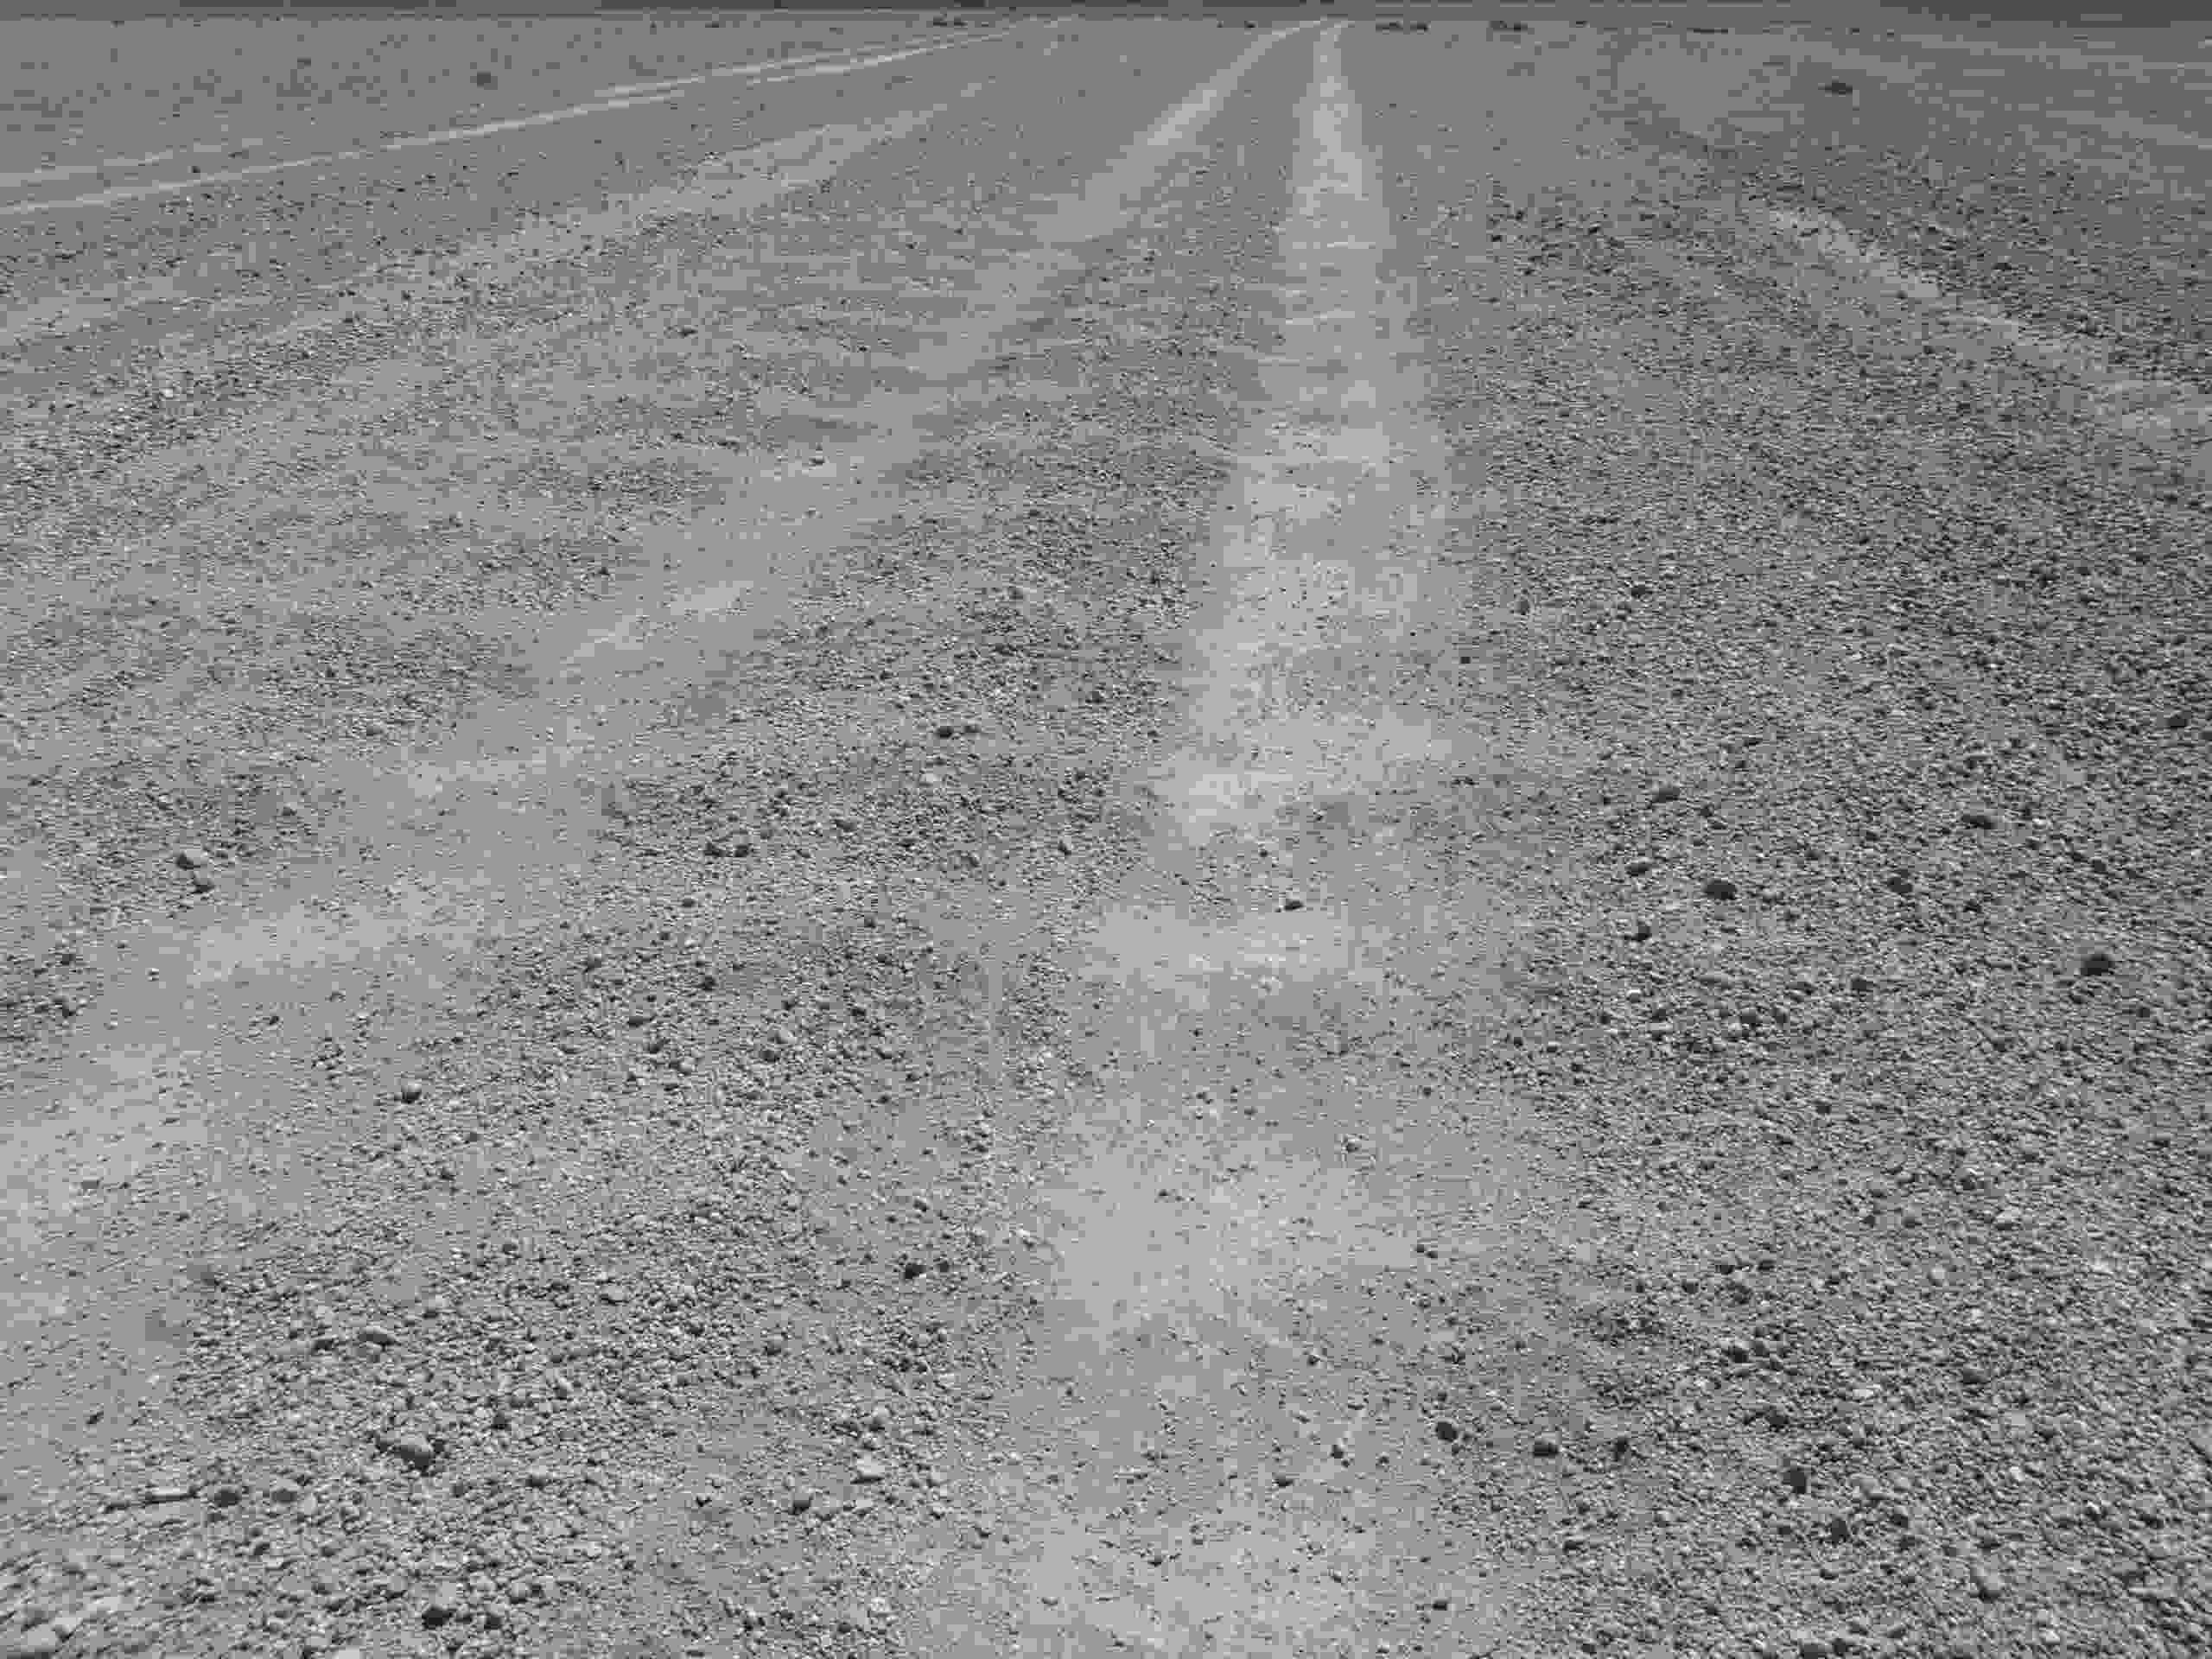
\includegraphics[width=\mywidth]{../wp-content/uploads/2015/04/wpid-wp-1427985527818.jpg} } 
 \newline
 On longe un dernier lac. \newline
 \newline
\centerline{\includegraphics[width=\mywidth]{../wp-content/uploads/2015/04/wpid-wp-1427985559421.jpg} } 
 \newline
 \newline
\centerline{\includegraphics[width=\mywidth]{../wp-content/uploads/2015/04/wpid-wp-1427985574067.jpg} } 
 \newline
 Au moment de rejoindre la première route en bon état depuis un moment, on se fait dépasser par un cycliste anglais : c'est seulement son 5e jour depuis San Pedro. \newline
 Dans la foulée on rencontre 2 autres cyclistes qui empruntent la route principale : quasiment un peloton pendant quelques kilomètres ! \newline
 \newline
\centerline{\includegraphics[width=\mywidth]{../wp-content/uploads/2015/04/wpid-wp-1427985593533.jpg} } 
 \newline
 \newline
\centerline{\includegraphics[width=\mywidth]{../wp-content/uploads/2015/04/wpid-wp-1427985630834.jpg} } 
 \newline
 La journée se termine par un dernier petit col à 4200m. \newline
 \newline
\centerline{\includegraphics[width=\mywidth]{../wp-content/uploads/2015/04/wpid-wp-1427985662568.jpg} } 
 \newline
 9e jour : \newline
 Longue descente dans le sable. \newline
 \newline
\centerline{\includegraphics[width=\mywidth]{../wp-content/uploads/2015/04/wpid-wp-1427985680592.jpg} } 
 \newline
 \newline
\centerline{\includegraphics[width=\mywidth]{../wp-content/uploads/2015/04/wpid-wp-1427985709669.jpg} } 
 \newline
 \newline
\centerline{\includegraphics[width=\mywidth]{../wp-content/uploads/2015/04/wpid-wp-1427985731653.jpg} } 
 \newline
 Traversée d'un petit salar. \newline
 \newline
\centerline{\includegraphics[width=\mywidth]{../wp-content/uploads/2015/04/wpid-wp-1427985755004.jpg} } 
 \newline
 À la pause de midi on croise un cycliste autrichien. Pour lui c'est le début, bon courage ! \newline
 \newline
\centerline{\includegraphics[width=\mywidth]{../wp-content/uploads/2015/04/wpid-wp-1427985769783.jpg} } 
 \newline
 Du plat pour finir la journée le long des champs de quinoa, on est bien en Bolivie. \newline
 \newline
\centerline{\includegraphics[width=\mywidth]{../wp-content/uploads/2015/04/wpid-wp-1427985789893.jpg} } 
 \newline
 La traversée du Sud Lipez se termine dans le village de San Juan. \newline
 \newline
\centerline{\includegraphics[width=\mywidth]{../wp-content/uploads/2015/04/wpid-wp-1427985851009.jpg} } 
 \newline
 Un poulet frites riz le plat numéro 1 en Bolivie : ça change des pâtes, sauce tomate, thon… \newline
 \newline
\centerline{\includegraphics[width=\mywidth]{../wp-content/uploads/2015/04/wpid-wp-1427985818141.jpg} } 
 \newline

\newpage
 
